\documentclass[a4paper,12pt]{article}
\usepackage[utf8]{inputenc}
\usepackage[T1]{fontenc}
\usepackage[italian]{babel}
\usepackage[sfdefault]{atkinson}
\renewcommand*\familydefault{\sfdefault}
\usepackage{float}
\usepackage{microtype}
\usepackage{geometry}
\usepackage{setspace}
\usepackage{enumitem}
\usepackage{titlesec}
\usepackage{chngpage}
\usepackage{tocloft}
\usepackage{longtable}
\usepackage{ltablex}
\usepackage{array}
\usepackage{xstring}
\usepackage{graphicx}
\usepackage{fancyhdr}
\usepackage[table]{xcolor}
\usepackage{color,soul}
\usepackage[most]{tcolorbox}
\usepackage{nameref}
\usepackage[colorlinks=true]{hyperref}

% --- INSERISCI QUESTO NEL PREAMBOLO DEL TUO DOCUMENTO ---
\usepackage{amssymb} % per il simbolo \checkmark
\usepackage{pifont}

% Macro per semplificare e alleggerire il codice della tabella
\newcommand{\ok}{\begin{center}S\end{center}}
\newcommand{\ko}{\textcolor{red!80!black}{$\times$ Mancante}}
\newcommand{\warn}[1]{\textcolor{orange!90!black}{\textbf{!} Multiplo (#1)}}
% Use URL-style line breaking to keep long test file names inside table borders.
\newcommand{\f}[1]{\nolinkurl{#1}\newline}
\newcommand{\q}[1]{\textit{#1}}
\newcommand{\sep}{\newline \vspace{2mm} \hrule \vspace{2mm}}
\newcommand{\testdesc}[1]{%
    \begingroup
    \StrBehind{#1}{] }[\testdesctmp]%
    \StrGobbleRight{\testdesctmp}{1}[\testdesctmp]%
    \textit{\testdesctmp}%
    \endgroup
}
% --------------------------------------------------------

% Colori ZPUS - Verde, Nero, Bianco
\definecolor{zpusgreen}{RGB}{4, 138, 55}
\definecolor{zpusdarkgreen}{RGB}{0, 100, 0}
\definecolor{zpusblack}{RGB}{0, 0, 0}
\definecolor{zpuswhite}{RGB}{255, 255, 255}
\definecolor{zpuslightgray}{RGB}{245, 245, 245}

\hypersetup{
    linkcolor=black,
    urlcolor=blue
}

\definecolor{lightblack}{gray}{0.35}
\newcommand{\glossario}[1]{\textit{#1}\textsubscript{\textbf{\textit{\textcolor{lightblack}{G}}}}}
\newcommand{\ped}[1]{\textsubscript{#1}}

\newcommand{\testoutputs}[1]{\begin{itemize}[leftmargin=*,nosep,topsep=0pt,itemsep=0pt]#1\end{itemize}}

\pagestyle{fancy}
\setlength{\headwidth}{\textwidth}
\fancyhfoffset[L,R]{0pt}
\lhead{\rightmark}
\rhead{7-ZPUs}
\lfoot{Piano di Qualifica}
\rfoot{\thepage}
\cfoot{}
\renewcommand{\headrulewidth}{0.8pt}
\renewcommand{\footrulewidth}{0.8pt}

\renewcommand{\contentsname}{Indice}
\renewcommand{\listoftables}{Elenco delle tabelle}
\renewcommand{\listoffigures}{Elenco delle immagini}

\geometry{margin=2.5cm}
\setstretch{1.1}

\titleclass{\subsubsubsection}{straight}[\subsection]

\newcounter{subsubsubsection}[subsubsection]
\renewcommand\thesubsubsubsection{\thesubsubsection.\arabic{subsubsubsection}}
\renewcommand\theparagraph{\thesubsubsubsection.\arabic{paragraph}} % optional; useful if paragraphs are to be numbered

\titleformat{\subsubsubsection}
  {\normalfont\normalsize\bfseries}{\thesubsubsubsection}{1em}{}
\titlespacing*{\subsubsubsection}
{0pt}{3.25ex plus 1ex minus .2ex}{1.5ex plus .2ex}

\makeatletter
\renewcommand\paragraph{\@startsection{paragraph}{5}{\z@}%
  {3.25ex \@plus1ex \@minus.2ex}%
  {-1em}%
  {\normalfont\normalsize\bfseries}}
\renewcommand\subparagraph{\@startsection{subparagraph}{6}{\parindent}%
  {3.25ex \@plus1ex \@minus .2ex}%
  {-1em}%
  {\normalfont\normalsize\bfseries}}
\def\toclevel@subsubsubsection{4}
\def\toclevel@paragraph{5}
%\def\toclevel@paragraph{6}
\def\toclevel@subparagraph{6}
\def\l@subsubsubsection{\@dottedtocline{4}{7em}{4em}}
\def\l@paragraph{\@dottedtocline{5}{10em}{5em}}
\def\l@subparagraph{\@dottedtocline{6}{14em}{6em}}
\makeatother

\setcounter{secnumdepth}{4}
\setcounter{tocdepth}{4}

\titleformat{\section}{\LARGE\bfseries}{\thesection}{1em}{}
\titleformat{\subsection}{\Large\bfseries}{\thesubsection}{1em}{}
\titleformat{\subsubsection}{\large\bfseries}{\thesubsubsection}{1em}{}
\titleformat{\paragraph}{\large\bfseries}{\theparagraph}{1em}{}
\titleformat{\subparagraph}{\normalsize\bfseries}{\thesubparagraph}{1em}{}

\setlength\parindent{0pt}

\begin{document}

\begin{center}
    
\includegraphics[width=9.5cm]{../../assets/logo7zpus.jpg}\\
    \small\hspace{10cm} 7zpus.swe@gmail.com\\
    \vspace{0.5cm}
    \LARGE \textbf{Piano di Qualifica}\\
    \vspace{0.3cm}
    \normalsize \textbf{Versione:} 2.0.0\\
    \textbf{Responsabile:} Georgescu Diana \\
    	\textbf{Destinatari:} Sanmarco Informatica S.p.A., Prof. Tullio Vardanega, Prof. Riccardo Cardin, Team 7-ZPUs \\
\end{center}

\vspace{0.3cm}
\hrule
\vspace{0.5cm}


\section*{Tabella di Versionamento}
\begin{table}[H]
    \begin{adjustwidth}{-4cm}{-4cm}
    \centering
    \begin{tabular}{|c|c|c|c|c|}
        \hline
        \textbf{Versione} & \textbf{Data} & \textbf{Autore}  & \textbf{Verificatore} & \textbf{Descrizione} \\
        \hline
        2.0.0 & 2026/03/15 & Georgescu Diana & - & \begin{tabular}[c]{@{}c@{}} Approvazione finale\\ per revisione PB \end{tabular} \\
        \hline
        1.2.0 & 2026/03/15 & Vigolo Davide & Rocco Matteo A. & \begin{tabular}[c]{@{}c@{}} Aggiornamento piano\\ di qualifica \end{tabular} \\
        \hline
        1.1.0 & 2026/03/18 & Aaron Gingillino & Lorenzo Soligo & \begin{tabular}[c]{@{}c@{}} Aggiunta metriche di\\ cruscotto aggiuntive \end{tabular} \\
        \hline
        1.0.0 & 2025/02/13 & Laoud Zakaria & Vigolo Davide & \begin{tabular}[c]{@{}c@{}} Approvazione per \\baseline RTB \end{tabular} \\
        \hline
         0.4.0 & 2025/02/09 & Rocco Matteo A. & Gingillino Aaron & \begin{tabular}[c]{@{}c@{}} Aggiunta sezione\\ \glossario{test di sistema} \end{tabular} \\
        \hline
        0.3.0 & 2025/02/08 & Vigolo Davide & Soligo Lorenzo & \begin{tabular}[c]{@{}c@{}} Aggiunta sezione cruscotto \\ di valutazione \end{tabular} \\
        \hline
        0.2.0 & 2025/02/02 & Vigolo Davide & Soligo Lorenzo & \begin{tabular}[c]{@{}c@{}} Revisione metriche\\ e aggiornamento soglie \end{tabular} \\
        \hline
        0.1.0 & 2025/12/14 & Rocco Matteo A. & Vigolo Davide & \begin{tabular}[c]{@{}c@{}} Creazione del documento\\ e stesura iniziale \end{tabular} \\
        \hline
    \end{tabular}
    \end{adjustwidth}
\end{table}

\tableofcontents
\newpage

\listoftables
\newpage

\listoffigures
\newpage

\section{Introduzione}

\subsection{Scopo}
Questo documento definisce la strategia di \glossario{garanzia della qualità} del progetto, stabilendo gli obiettivi quantitativi per le attività di \glossario{verifica} e \glossario{validazione}. L'adozione di un approccio sistematico e misurabile è fondamentale per garantire due dimensioni interdipendenti:
\begin{itemize}
    \item Qualità di Processo: Per perseguire l'\glossario{efficienza} (uso ottimale delle risorse) e l'aderenza al \glossario{Way of Working}.
    \item Qualità di Prodotto: Per garantire l'\glossario{efficacia} (conformità ai \glossario{requisiti}).
\end{itemize}

Poiché il miglioramento del \glossario{processo} influisce sulla qualità del prodotto, e quest'ultima è condizione necessaria per la qualità in uso (il valore reale per il \glossario{committente}), il presente Piano di Qualifica si articola in tre componenti operative:
\begin{itemize}
    \item Piano della Qualità: Definisce gli obiettivi metrici, le risorse e le procedure necessarie per conseguirli.
    \item Controllo di Qualità: Assicura, tramite il Cruscotto di Valutazione, che i risultati intermedi soddisfino le attese passo-passo, monitorando l'andamento delle \glossario{metriche}.
    \item Miglioramento Continuo: Attua il ciclo PDCA (\glossario{Plan-Do-Check-Act}) per analizzare le misurazioni e introdurre azioni correttive o preventive sui processi.
\end{itemize}


\subsection{Glossario}
Ogni termine tecnico o con particolare significato nell'ambito dell'\glossario{Ingegneria del Software} utilizzato nella documentazione di progetto viene definito nell'apposito documento \href{https://7-zpus.github.io/Docs/assets/2_RTB/DocumentiInterni/Glossario.pdf}{\ul{Glossario}\setulcolor{blue}}\ped{(v1.0.0)}.

\subsection{Riferimenti}

\subsubsection{Riferimenti Normativi}
\begin{itemize}
    \item \href{https://7-zpus.github.io/Docs/assets/2_RTB/DocumentiInterni/NormeDiProgetto.pdf}{\ul{NormeDiProgetto}\setulcolor{blue}}\ped{(v1.0.0)}
    \item \href{https://www.math.unipd.it/~tullio/IS-1/2025/Progetto/C3.pdf}{\ul{Capitolato C3: DIPReader}\setulcolor{blue}} \ped{(ultimo accesso: 01/12/2025)}
    \item \href{https://www.math.unipd.it/~tullio/IS-1/2025/Dispense/PD1.pdf}{\ul{Regolamento di Progetto Didattico a.a. 2025/2026}\setulcolor{blue}} \ped{(ultimo accesso: 06/02/2026)}
\end{itemize}
\subsubsection{Riferimenti Informativi}
\begin{itemize}
    \item \href{https://7-zpus.github.io/Docs/assets/2_RTB/DocumentiInterni/Glossario.pdf}{\ul{Glossario}\setulcolor{blue}} \ped{(v1.0.0)}
    \item \href{https://iso25000.com}{\ul{The ISO/IEC 25000 Series of Standards}\setulcolor{blue}} \ped{(ultimo accesso: 06/02/2026)}
    \item \href{https://www.iso.org/standard/63712.html}{\ul{Standard ISO/IEC 9126-1:2001}\setulcolor{blue}} \ped{(ultimo accesso: 16/01/2026)}
    \item \href{https://www.iso.org/standard/71952.html}{\ul{Standard ISO/IEC 145981-1:1999}\setulcolor{blue}} \ped{(ultimo accesso: 06/02/2026)}
\end{itemize}

\section{Metriche di qualità}

\subsection{Qualità di processo}

\subsubsection{Processi primari}

\subsubsubsection{Fornitura}

\renewcommand{\arraystretch}{1.2}

\begin{table}[H]
    \centering
    \rowcolors{2}{gray!15}{white}
    \begin{tabular}{|c|c|c|c|}
        \hline
        \rowcolor{zpusgreen!30}
        \textbf{Codice} & \textbf{Nome metrica} & \begin{tabular}[c]{@{}c@{}}  \textbf{Valore}\\\textbf{accettabile} \end{tabular} & \begin{tabular}[c]{@{}c@{}}  \textbf{Valore}\\\textbf{desiderabile} \end{tabular} \\
        \hline
        MPC-1 & EV (Earned Value) & $\geq$0 & PV \\
        \hline
        MPC-2 & PV (Planned Value) & $\geq$0 & - \\
        \hline
        MPC-3 & AC (Actual Cost) & $\geq$0 & $\leq$EV \\
        \hline
        MPC-4 & CPI (Cost Performance Index) & $\geq$0.5 & $\geq$1 \\
        \hline
        MPC-5 & SPI (Schedule Performance Index) & $\geq$0.5 & $\geq$1 \\
        \hline
        MPC-6 & ETC (Estimate to Complete) & $\geq$0 & $\leq$BAC\textsubscript{\textit{G}} - AC\textsubscript{\textit{G}} \\
        \hline
        MPC-7 & EAC (Estimate at Completion) & $\geq$0 & $\leq$BAC \\
        \hline
    \end{tabular}
    \caption{Metriche di qualità di processo - Fornitura}
    \label{tab:PCPrim-Fornitura}
\end{table}

\subsubsubsection{Sviluppo}

\begin{table}[H]
    \centering
    \rowcolors{2}{gray!15}{white}
    \begin{tabular}{|c|c|p{3cm}|p{3cm}|}
        \hline
        \rowcolor{zpusgreen!30}
        \textbf{Codice} & \textbf{Nome metrica} & \begin{tabular}[c]{@{}c@{}}  \textbf{Valore}\\\textbf{accettabile} \end{tabular} & \begin{tabular}[c]{@{}c@{}}  \textbf{Valore}\\\textbf{desiderabile} \end{tabular} \\
        \hline
        MPC-8 & Deployment frequency & - & 1/settimana \\
        \hline
        MPC-9 & Requirements Stability Index & $\geq$70\% & 100\% \\
        \hline
        MPC-10 & Average build time & $\leq$3 min & $\leq$1 min \\
        \hline
        MPC-11 & SV (Sprint Velocity) & $\geq$80 \% SV medio ultimi N sprint & 90\% – 110\% SV medio ultimi N sprint \\
        \hline
        MPC-12 & Burndown Adherence & $\pm$1.6 o $\pm$0.7 & $\pm$1 \\
        \hline
    \end{tabular}
    \caption{Metriche di qualità di processo - Sviluppo}
    \label{tab:PCPrim-Sviluppo}
\end{table}

\subsubsection{Processi di supporto}

\subsubsubsection{Documentazione}

\begin{table}[H]
    \centering
    \rowcolors{2}{gray!15}{white}
    \begin{tabular}{|c|c|c|c|}
        \hline
        \rowcolor{zpusgreen!30}
        \textbf{Codice} & \textbf{Nome metrica} & \begin{tabular}[c]{@{}c@{}}  \textbf{Valore}\\\textbf{accettabile} \end{tabular} & \begin{tabular}[c]{@{}c@{}}  \textbf{Valore}\\\textbf{desiderabile} \end{tabular} \\
        \hline
        MPC-13 & Indice di Gulpease & $\geq$60 & $\geq$75\\
        \hline
        MPC-14 & Correttezza ortografica & 0 & 0 \\
        \hline
    \end{tabular}
    \caption{Metriche di qualità di processo - Documentazione}
    \label{tab:PCSupp-Documentazione}
\end{table}

\subsubsubsection{Verifica}

\begin{table}[H]
    \centering
    \rowcolors{2}{gray!15}{white}
    \begin{tabular}{|c|c|c|c|}
        \hline
        \rowcolor{zpusgreen!30}
        \textbf{Codice} & \textbf{Nome metrica} & \begin{tabular}[c]{@{}c@{}}  \textbf{Valore}\\\textbf{accettabile} \end{tabular} & \begin{tabular}[c]{@{}c@{}}  \textbf{Valore}\\\textbf{desiderabile} \end{tabular} \\
        \hline
        MPC-15 & Code review turnaround time & $\leq$72h & $\leq$24h\\
        \hline
        MPC-16 & Test success rate & 100\% & 100\%\\
        \hline
        MPC-17 & Code Coverage & $\geq$70\% & $\geq$80\% \\
        \hline
    \end{tabular}
    \caption{Metriche di qualità di processo - Verifica}
    \label{tab:PCSupp-Verifica}
\end{table}

\subsubsection{Processi organizzativi}

\subsubsubsection{Gestione dei rischi}

\begin{table}[H]
    \centering
    \rowcolors{2}{gray!15}{white}
    \begin{tabular}{|c|c|c|c|}
        \hline
        \rowcolor{zpusgreen!30}
        \textbf{Codice} & \textbf{Nome metrica} & \begin{tabular}[c]{@{}c@{}}  \textbf{Valore}\\\textbf{accettabile} \end{tabular} & \begin{tabular}[c]{@{}c@{}}  \textbf{Valore}\\\textbf{desiderabile} \end{tabular} \\
        \hline
        MPC-18 & Rischi non previsti & $\geq$0 & 0\\
        \hline
    \end{tabular}
    \caption{Metriche di qualità di processo - Gestione dei rischi}
    \label{tab:PCOrg-GestioneRischi}
\end{table}

\subsubsubsection{Gestione della Qualità}
\begin{table}[H]
    \centering
    \rowcolors{2}{gray!15}{white}
    \begin{tabular}{|c|c|c|c|}
        \hline
        \rowcolor{zpusgreen!30}
        \textbf{Codice} & \textbf{Nome metrica} & \begin{tabular}[c]{@{}c@{}}  \textbf{Valore}\\\textbf{accettabile} \end{tabular} & \begin{tabular}[c]{@{}c@{}}  \textbf{Valore}\\\textbf{desiderabile} \end{tabular} \\
        \hline
        MPC-19 & Metriche soddisfatte & $\geq$70\% & 100\% \\
        \hline
    \end{tabular}
    \caption{Metriche di qualità di prodotto - Gestione della Qualità}
    \label{tab:PCOrg-GestioneQualità}
\end{table}


\subsection{Qualità di prodotto}
Le metriche definite in questa sezione riguardano principalmente caratteristiche di qualità "interne" del prodotto software. Raggiungere la qualità su queste caratteristiche abilita all'ottenimento di qualità in uso, o "esterna".
Suddividiamo le metriche secondo raggruppamenti logici qui di seguito elencati ed esplicitati:
\begin{itemize}
    \item \textbf{Funzionalità}: completezza, correttezza ed appropriatezza del prodotto
    \item \textbf{Affidabilità}: maturità, disponibilità, tolleranza ai guasti e riparabilità del prodotto
    \item \textbf{Usabilità}: apprendibilità, operabilità, UX e accessibilità del prodotto
    \item \textbf{Efficienza}: nel tempo, nelle altre risorse, nella capacità
    \item \textbf{Manutenibilità}: modularità, riusabilità, analizzabilità, modificabilità e verificabilità del prodotto
    \item \textbf{Portabilità}: adattabilità del prodotto a diversi ambienti
\end{itemize}


\subsubsection{Funzionalità}

\begin{table}[H]
    \centering
    \rowcolors{2}{gray!15}{white}
    \begin{tabular}{|c|c|c|c|}
        \hline
        \rowcolor{zpusgreen!30}
        \textbf{Codice} & \textbf{Nome metrica} & \begin{tabular}[c]{@{}c@{}}  \textbf{Valore}\\\textbf{accettabile} \end{tabular} & \begin{tabular}[c]{@{}c@{}}  \textbf{Valore}\\\textbf{desiderabile} \end{tabular} \\
        \hline
        MPD-1 & Requisiti obbligatori soddisfatti & $\geq$0\% & 100\% \\
        \hline
        MPD-2 & Requisiti opzionali soddisfatti & $\geq$0\% & 100\%\\
        \hline
        MPD-3 & Requisiti desiderabili soddisfatti & $\geq$0\% & 100\% \\
        \hline
    \end{tabular}
    \caption{Metriche di qualità di prodotto - Funzionalità}
    \label{tab:MPD-funzionalità}
\end{table}


\subsubsection{Affidabilità}

\begin{table}[H]
    \centering
    \rowcolors{2}{gray!15}{white}
    \begin{tabular}{|c|c|c|c|}
        \hline
        \rowcolor{zpusgreen!30}
        \textbf{Codice} & \textbf{Nome metrica} & \begin{tabular}[c]{@{}c@{}}  \textbf{Valore}\\\textbf{accettabile} \end{tabular} & \begin{tabular}[c]{@{}c@{}}  \textbf{Valore}\\\textbf{desiderabile} \end{tabular} \\
        \hline
        MPD-4 & Broken Links & 2 & 0\\
        \hline
        MPD-5 & Branch coverage & $\geq$80\% & $\geq$90\% \\
        \hline
        MPD-6 & Statement Coverage & $\geq$65\% & $\geq$80\% \\
        \hline
    \end{tabular}
    \caption{Metriche di qualità di prodotto - Affidabilità}
    \label{tab:MPD-affidabilità}
\end{table}

\subsubsection{Usabilità}

\begin{table}[H]
    \centering
    \rowcolors{2}{gray!15}{white}
    \begin{tabular}{|c|c|c|c|}
        \hline
        \rowcolor{zpusgreen!30}
        \textbf{Codice} & \textbf{Nome metrica} & \begin{tabular}[c]{@{}c@{}}  \textbf{Valore}\\\textbf{accettabile} \end{tabular} & \begin{tabular}[c]{@{}c@{}}  \textbf{Valore}\\\textbf{desiderabile} \end{tabular} \\
        \hline
        MPD-7 & Profondità di navigazione & $\geq$0 & $\leq$5 \\
        \hline
    \end{tabular}
    \caption{Metriche di qualità di prodotto - Usabilità}
    \label{tab:MPD-usabilità}
\end{table}


\subsubsection{Efficienza}

\begin{table}[H]
    \centering
    \rowcolors{2}{gray!15}{white}
    \begin{tabular}{|c|c|c|c|}
        \hline
        \rowcolor{zpusgreen!30}
        \textbf{Codice} & \textbf{Nome metrica} & \begin{tabular}[c]{@{}c@{}}  \textbf{Valore}\\\textbf{accettabile} \end{tabular} & \begin{tabular}[c]{@{}c@{}}  \textbf{Valore}\\\textbf{desiderabile} \end{tabular} \\
        \hline
        MPD-8 & Indexing Time & 2min & $\leq$30 s \\
        \hline
        MPD-9 & Search Time & $\leq$2 s & $\leq$1 s \\
        \hline
        MPD-10 & Average CPU usage & $\leq$30\% & $\leq$15\% \\
        \hline
        MPD-11 & Peak memory usage & $\leq$1 GB & $\leq$500 MB \\
        \hline
    \end{tabular}
    \caption{Metriche di qualità di prodotto - Efficienza}
    \label{tab:MPD-efficienza}
\end{table}



\subsubsection{Manutenibilità}

\begin{table}[H]
    \centering
    \rowcolors{2}{gray!15}{white}
    \begin{tabular}{|c|c|c|c|}
        \hline
        \rowcolor{zpusgreen!30}
        \textbf{Codice} & \textbf{Nome metrica} & \begin{tabular}[c]{@{}c@{}}  \textbf{Valore}\\\textbf{accettabile} \end{tabular} & \begin{tabular}[c]{@{}c@{}}  \textbf{Valore}\\\textbf{desiderabile} \end{tabular} \\
       \hline
        MPD-12 & Complessità ciclomatica & $\leq$15 & $\leq$10 \\
        \hline
        MPD-13 & Accoppiamento tra classi & $\leq$10 & $\leq$5 \\
        \hline
        MPD-14 & Code Smells & $\leq$15 & 0 \\
        \hline
    \end{tabular}
    \caption{Metriche di qualità di prodotto - Manutenibilità}
    \label{tab:MPD-manutenibilità}
\end{table}

\subsubsection{Portabilità}


\begin{table}[H]
    \centering
    \rowcolors{2}{gray!15}{white}
    \begin{tabular}{|c|c|c|c|}
        \hline
        \rowcolor{zpusgreen!30}
        \textbf{Codice} & \textbf{Nome metrica} & \begin{tabular}[c]{@{}c@{}}  \textbf{Valore}\\\textbf{accettabile} \end{tabular} & \begin{tabular}[c]{@{}c@{}}  \textbf{Valore}\\\textbf{desiderabile} \end{tabular} \\
        \hline
        MPD-15 & Sistemi operativi supportati & 3 & $\geq$3 \\
        \hline
    \end{tabular}
    \caption{Metriche di qualità di prodotto - Portabilità}
    \label{tab:MPD-portabilità}
\end{table}

\iffalse\subsection{Test di integrazione}

\setlength{\LTleft}{-0.4cm}
\renewcommand{\arraystretch}{1.2}
\rowcolors{2}{gray!15}{white}
\begin{longtable}{|p{2.5cm}|p{2.0cm}|p{10.5cm}|}
\hline
\rowcolor{zpusgreen!30}
\textbf{ID Test} & \textbf{Stato} & \textbf{Posizioni (File e Titolo)} \\
\hline
\endfirsthead
\rowcolor{zpusgreen!30}
\textbf{ID Test} & \textbf{Stato} & \textbf{Posizioni (File e Titolo)} \\
\hline
\endhead
IT-C-001 & \ok & \f{core/test/dao/query/DocumentMetadataQueryBuilder.integration.spec.ts}                              \\ 
\hline
IT-C-002 & \ok & \f{core/test/repo/impl/LocalPackageReaderAdapter.integration.test.ts}                                 \\ 
\hline
IT-C-003 & \ok & \f{core/test/services/impl/IntegrityVerificationService.integration.spec.ts}                          \\ 
\hline
IT-C-004 & \ok & \f{core/test/use-case/search/SearchUseCases.integration.spec.ts}                                      \\ 
\hline
IT-C-005 & \ok & \f{core/test/use-case/utils/indexing/impl/IndexDip.integration.spec.ts}                               \\ 
\hline
IT-R-001 & \ok & \f{renderer/src/app/features/search/adapters/indexing-ipc-gateway.spec.ts}                            \\ 
\hline
IT-R-002 & \ok & \f{renderer/src/app/features/search/integration test/advanced-filter-panel.integration.spec.ts}       \\ 
\hline
IT-R-003 & \ok & \f{renderer/src/app/features/search/integration test/facade-validation.integration.spec.ts}           \\ 
\hline
IT-R-004 & \ok & \f{renderer/src/app/features/search/integration test/facade-validation-mock-serv.integration.spec.ts} \\ 
\hline
IT-R-005 & \ok & \f{renderer/src/app/features/search/integration test/filter-validator.integration.spec.ts}            \\ 
\hline
IT-R-006 & \ok & \f{renderer/src/app/features/search/integration test/result-redirecting.integration.spec.ts}          \\ 
\hline
IT-R-007 & \ok & \f{renderer/src/app/features/search/integration test/search-flow.integration.spec.ts}                 \\ 
\hline
IT-R-008 & \ok & \f{renderer/src/app/features/verification/integration/integrity-end-to-end.integration.spec.ts}       \\ 
\hline
IT-R-009 & \ok & \f{renderer/src/app/features/navigation/integration/navigation-empty-state.integration.spec.ts}       \\ 
\hline
\rowcolor{white}
\caption{Report test di integrazione}
\label{tab:test-integrazione}
\end{longtable}

\fi

\section{Cruscotto di valutazione e miglioramento}

Il Cruscotto di Valutazione della qualità costituisce lo strumento operativo fondamentale per il monitoraggio e il controllo del progetto. Esso traduce la strategia di verifica e gli obiettivi quantitativi attesi in misurazioni effettive, permettendo di valutare due dimensioni distinte:
\begin{itemize}
    \item Qualità di Processo: per misurare l'efficienza (uso delle risorse) e l'aderenza al \textit{Way of Working} attraverso le metriche di processo (MPC).
    \item Qualità di Prodotto: per verificare l'efficacia (conformità ai requisiti) del software prodotto attraverso le metriche di prodotto (MPD).
\end{itemize}

L'obiettivo non è la semplice rendicontazione, ma l'attuazione del ciclo di miglioramento continuo PDCA (\textit{Plan-Do-Check-Act}). Per questo motivo, i grafici seguenti riportano misurazioni a cadenza settimanale: un monitoraggio limitato al solo termine di periodo risulterebbe una scelta miope, mentre un'analisi costante permette di individuare tempestivamente criticità e intervenire proattivamente sui rischi.\\

\noindent \ul{Nota}: Si segnala che nel primo periodo, in fase di definizione del \textit{Way of Working}, il gruppo non disponeva ancora del cruscotto operativo. Tuttavia, le metriche relative sono state calcolate retroattivamente e riportate per garantire la completezza storica e l'analisi dei trend.

\subsection{MPC-1, MPC-2, MPC-3: Earned Value, Planned Value, Actual Cost} \label{crsc_ev_pv_ac}
\begin{figure}[H]
    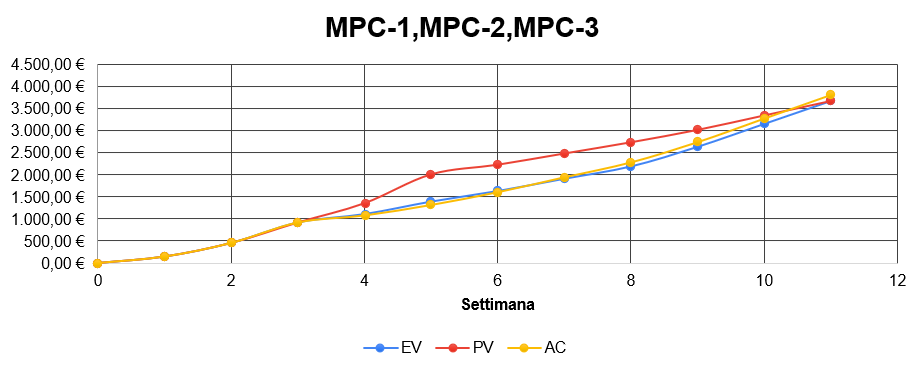
\includegraphics[width=\textwidth]{../../assets/pdq/ev_pv_ac.png}
    \caption{MPC-1, MPC-2, MPC-3: Earned Value, Planned Value, Actual Cost}
    \label{ev_pv_ac}
\end{figure}

\paragraph{RTB - Requirements And Technology Baseline}

Dal grafico si può apprezzare come il progetto sia partito lentamente
durante le prime due settimane, dovuto ovviamente alle fasi iniziali di 
organizzazione del gruppo. Successivamente durante il terzo e il quarto 
\glossario{Sprint} si può notare una differenza importante tr PV ed EV. 
Questo, come riportato nelle retrospettive, è dovuto ad una stima delle 
attività troppo ottimistica. Il gruppo ha intrapreso dunque un approccio 
più conservativo che ha portato al ricongiungersi dei due valori alla 
settimana 10-11. La differenza tra costo preventivato e attuale è rimasta
abbastanza contenuta. Unico scostamento avviene nelle ultime due settimane,
dove alcune attività hanno superato i costi preventivati a causa di prolungamenti nell'implementazione
di una funzionalità nel PoC. Questo scostamento è dovuto al fatto che i membri del
gruppo stanno di fatto esplorando tecnologie nuove e dunque i tempi di implementazione
possono fluttuare notevolmente.\\

\paragraph{PB - Product Baseline}

Dallo sprint 6 (settimana 14), compatibilmente con il termine della sessione d'esami, il carico di lavoro è aumentato
sostanzialmente in quanto il gruppo ha potuto dedicare tutto il tempo settimanale disponibile al progetto,
portando ad un incremento di tutti e tre i valori. Inoltre, durante questo periodo la gestione delle 
attività è migliorata in quanto il way of working è stato consolidato e appreso a pieno dai vari membri del gruppo.
Questo risulta in valori di EV,PV e AC molto più vicini tra loro, come si può apprezzare dal grafico.
Degno di nota è il rallentamento durante la settimana 20-21, poi riassorbito nello sprint successivo.

\subsection{MPC-4, MPC-5: CPI, SPI}
\begin{figure}[H]
    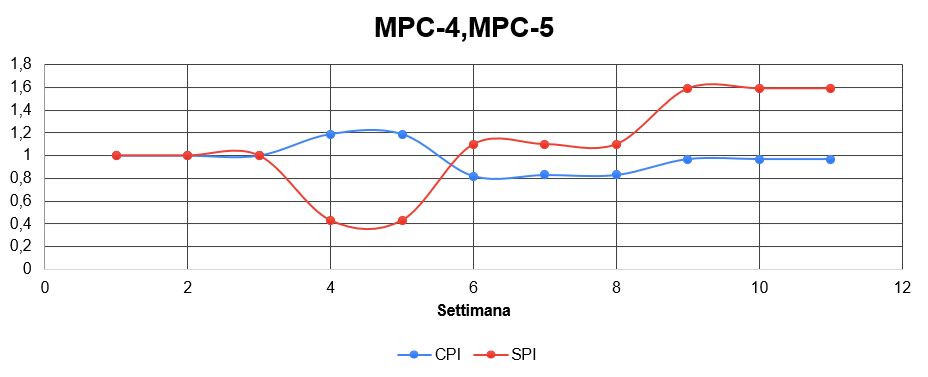
\includegraphics[width=\textwidth]{../../assets/pdq/cpi_spi.png}
    \caption{MPC-4, MPC-5: CPI, SPI}
    \label{cpi_spi}
\end{figure}

\paragraph{RTB - Requirements And Technology Baseline}

Dall'analisi di CPI e SPI emerge chiaramente la pianificazione inizialmente
troppo ottimistica, evidenziata dal calo dello SPI nelle settimane 3-5.
Nonostante il rallentamento, il gruppo ha completato le attività con costi
inferiori al previsto. A partire dalla settimana 6, si è osservato un recupero
progressivo del ritardo: lo SPI è tornato sopra 1 (dovuto al recupero delle task arretrate),
sebbene con un incremento dei costi. Il CPI si è successivamente stabilizzato nelle 
settimane 9-11, riflettendo una migliore consapevolezza circa la necessità di rivedere
la strategia di pianificazione. Nelle ultime due settimane si sono registrati errori
nella gestione dei preventivi e consuntivi di periodo, con conseguente aumento dei
costi associati alle attività. Le attività nelle ultime due settimane risultano
terminate per tempo. \\

\paragraph{PB - Product Baseline}

Dallo sprint 6 (settimana 14) fino al termine del progetto si può notare come i valori di CPI e SPI
siano molto più stabili. E' stato migliorato e consolidato infatti quanto appreso durante gli sprint precedenti.
Il gruppo ha intrapreso un approccio più conservativo che si è rivelato efficace, portando a valori di CPI e SPI tendenti ad 1, salvo qualche piccola fluttuazione.
Nello specifico, il CPI mostra come le stime orarie per le singole task sono migliorate, questo dovuto all'esperienza acquisita durante la fase di RTB.
D'altra parte lo SPI mostra come il gruppo abbia migliorato la capacità di pianificazione, nessuna task è stata riassegnata allo sprint successivo, mantenendo il valore costante ad 1.
\subsection{MPC-7: EAC confrontato con BAC}
\begin{figure}[H]
    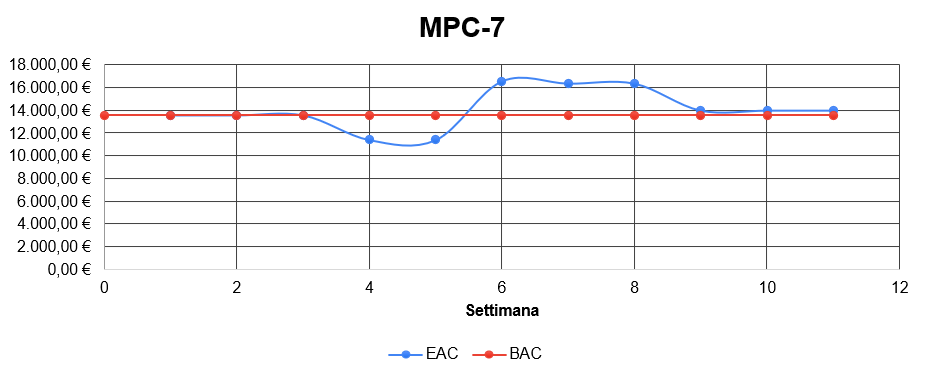
\includegraphics[width=\textwidth]{../../assets/pdq/eac_bac.png}
    \caption{MPC-7: EAC confrontato con BAC}
    \label{eac_bac}
\end{figure}

\paragraph{RTB - Requirements And Technology Baseline}

Strettamente collegato, e conseguenza del CPI, è l'andamento di EAC e BAC.
Tra le settimane 3 e 5 si osserva una diminuzione. Tale diminuzione tuttavia non
tiene conto del rinvio delle attività. Per quelle completate, il costo reale è
risultato inferiore. Una diminuzione della metrica EAC non significa dunque per forza
un miglioramento. Successivamente l'EAC aumenta, segnalando un incremento rispetto ai costi preventivati.
Questo aumento è dovuto alle numerose iterazioni, a volte molto distruttive,
sul documento di Analisi dei Requisiti. Dopo gli incontri con il prof.
Cardin il gruppo ha dovuto rivedere quasi completamente la struttura degli
\glossario{Use Case}. Allo stato attuale la pianificazione è ancora oggetto
di discussione all'interno del gruppo, in ottica di contenere il più possibile le fluttuazioni.\\

\paragraph{PB - Product Baseline}

Dallo sprint 6 (settimana 14), compatibilmente con quanto detto riguardo a MPC-4, il valore di Estimate At Completion
si è stabilizzato sul valore di Budget At Completion, indicando dunque un miglioramento nella gestione del budget.

\subsection{MPC-1, MPC-2, MPC-3, MPC-6, MPC-7: EV, PV, AC, EAC, ETC}
\begin{figure}[H]
    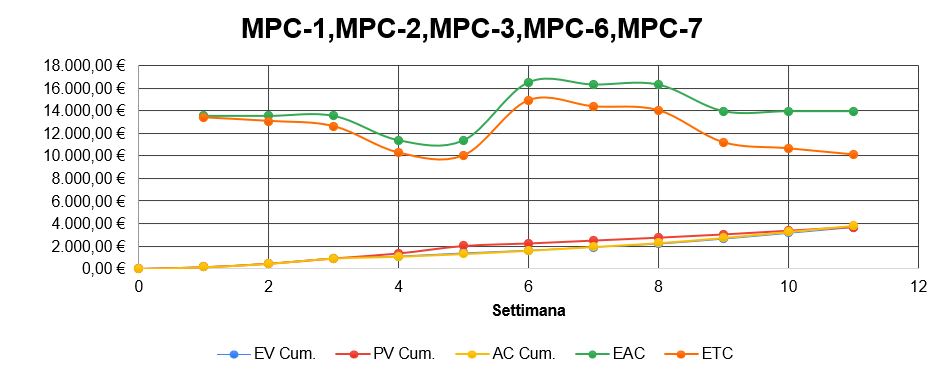
\includegraphics[width=\textwidth]{../../assets/pdq/ev_pv_ac_eac_etc.png}
    \caption{MPC-1, MPC-2, MPC-3, MPC-6, MPC-7: EV, PV, AC, EAC, ETC}
    \label{ev_pv_ac_eac_etcs}
\end{figure}

\paragraph{RTB - Requirements And Technology Baseline}

Si può apprezzare dal grafico un quadro generale di quanto detto fino ad ora.
Si osserva un aumento dell EAC nella fase iniziale, con un suo successivo rientro
e un lieve rialzo nelle ultime due settimane. \\

\paragraph{PB - Product Baseline}

Nel periodo conclusivo del progetto, il grafico evidenzia il pieno raggiungimento 
della stabilità operativa. La convergenza pressoché totale tra EV, PV e AC conferma 
l'efficacia del way of working adottato nella fase di Product Baseline: in termini 
pratici, l'assenza di scostamenti indica che le ultime funzionalità sono state 
implementate senza le fluttuazioni di costo e tempo che avevano caratterizzato 
le sperimentazioni tecnologiche iniziali.

L'appiattimento dell'EAC segnala il superamento definitivo 
delle incertezze, traducendosi in una proiezione di costo finale ormai 
certa e priva di rischi residui. Questo consolidamento è corroborato dal trend 
dell'ETC, che dalla settimana 15 scende con regolarità fino all'azzeramento finale; 
tale variazione riflette la capacità del gruppo di evadere le unità di lavoro 
rimanenti secondo una cadenza lineare, garantendo un atterraggio del progetto 
perfettamente in linea con le ultime stime di budget e tempistiche.

\subsection{MPC-8: Deployment frequency}
\begin{figure}[H]
    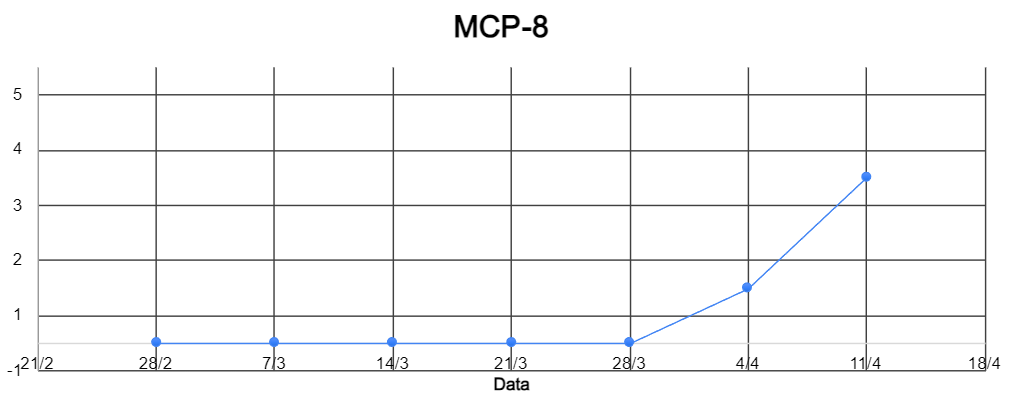
\includegraphics[width=\textwidth]{../../assets/pdq/deploy.png}
    \caption{MPC-8: Deployment frequency}
    \label{deployment_frequency}
\end{figure}
\paragraph{PB - Product Baseline}
Il deployment è avvenuto, come era naturale che fosse, nelle fasi finali del progetto. Il gruppo ha effettuato il primo deployment una volta effettuato la prima integrazione dei componenti. Il successivo deployment è stato in corrispondenza dell'incontro con la proponente il giorno 9 di Aprile. In seguito alle modifiche proposte dall'azienda, è stato effettuato un terzo deployment, che ha portato alla versione finale del PoC. In questo ultimo caso, le release sono state pubblicate in versione eseguibile anche per Windows e MacOs, oltre che per Linux.\\

\subsection{MPC-9: Requirements Stability Index}
\begin{figure}[H]
    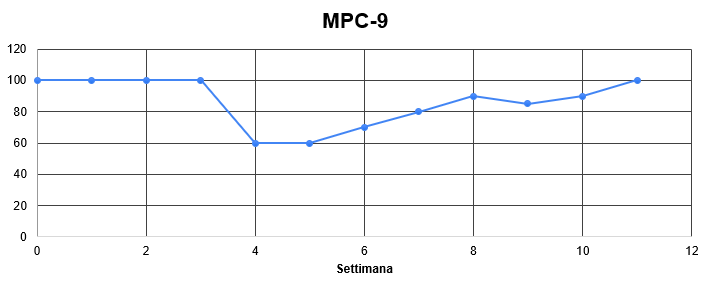
\includegraphics[width=\textwidth]{../../assets/pdq/rsi.png}
    \caption{MPC-9: Requirements Stability Index}
    \label{rsi}
\end{figure}
\paragraph{RTB - Requirements And Technology Baseline}
Dal grafico si osserva che, all'inizio, la stabilità dei requisiti è rimasta costante mentre il gruppo definiva le Norme di Progetto e i requisiti non erano ancora esplorati. Successivamente si è verificato un calo significativo: l'attenzione si è spostata sullo studio del dominio applicativo e sulle aspettative della \glossario{proponente}. 
La scarsa conoscenza del dominio e la continua selezione e revisione dei requisiti, anche per motivi di fattibilità, hanno generato instabilità. La proponente non ha imposto vincoli rigidi sulle funzionalità; di conseguenza i requisiti sono stati proposti e discussi in modo progressivo. 
Questo ha fatto sì che non si sia reso spesso necessario modificare, aggiungere o eliminare requisiti, e l'indice si è stabilizzato nella fase finale. Nella dodicesima settimana sono stati aggiunti dei requisiti per raggiungere il massimo livello di dettaglio, portando ad un lieve calo della metrica. \\
\paragraph{PB - Product Baseline}
Una correzione è stata però necessaria in seguito alla revisione da parte del professor Cardin, portando ad un'analisi più precisa per quanto riguarda i requisiti non funzionali. In questo caso, è stato necessario modificare alcuni requisiti funzionali per garantire la coerenza con i requisiti non funzionali, portando ad un calo dell'indice.\\
In seguito a questa modifiche i requisiti sono rimasti stabili, con un indice che si è mantenuto costante fino alla fine del progetto.\\


\subsection{MPC-10: Average build time}
\begin{figure}[H]
    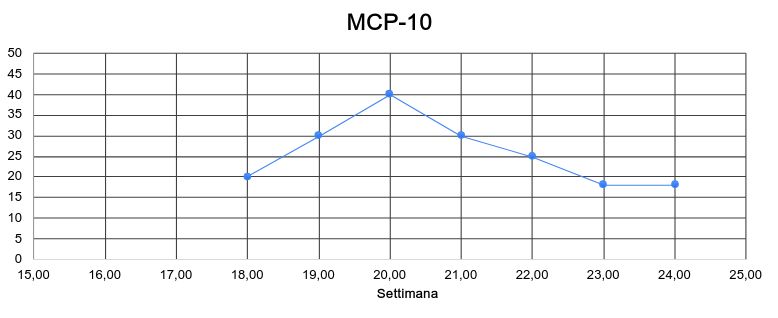
\includegraphics[width=\textwidth]{../../assets/pdq/avg_build_time.png}
    \caption{MPC-10: Average build time}
    \label{avg_build_time}
\end{figure}
\paragraph{PB - Product Baseline}
Dal grafico si osserva un aumento del tempo di build, dovuto all'aumento di complessità del progetto e alla crescita del numero di componenti. 
Il gruppo ha poi ridotto il tempo di build, ottimizzando le configurazioni e i processi di build a partire dalla settimana 21.

\subsection{MPC-11: Sprint Velocity}
\begin{figure}[H]
    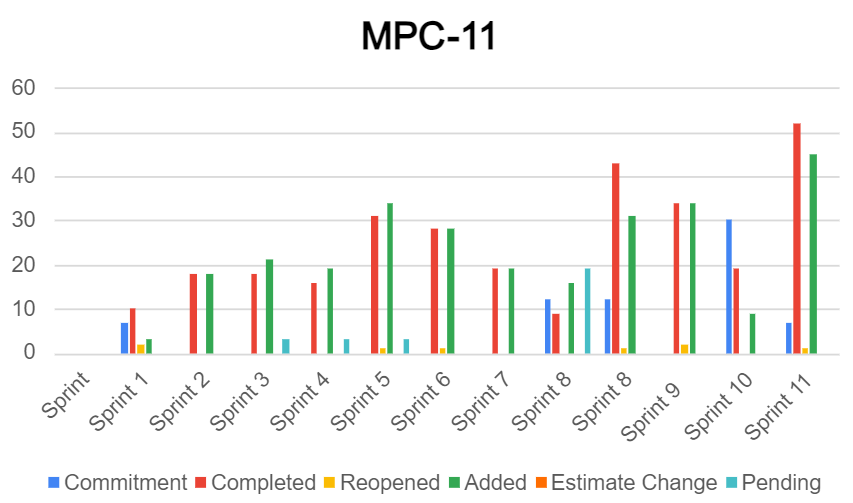
\includegraphics[width=\textwidth]{../../assets/pdq/sprint_velocity.png}
    \caption{MPC-11: Sprint Velocity}
    \label{sv}
\end{figure}
\paragraph{PB - Product Baseline}
La Sprint Velocity permette di misurare la quantità di lavoro completata durante uno sprint. Vediamo che il gruppo ha aumentato la produttività nel corso del progetto fino allo sprint 5. C'è stato in seguito, un calo di produttività che è da attribuire alle vacanze natalizie per lo sprint 6 e la sessione per lo sprint 7. Entrambi fattori di rischio previsti.\\
Un ulteriore aumento è stato registrato in corrispondenza dell'avvicinamento alla data prevista per la consegna, con un picco nello sprint 11.\\

\subsection{MPC-12: Burndown Chart}
\begin{figure}[H]
    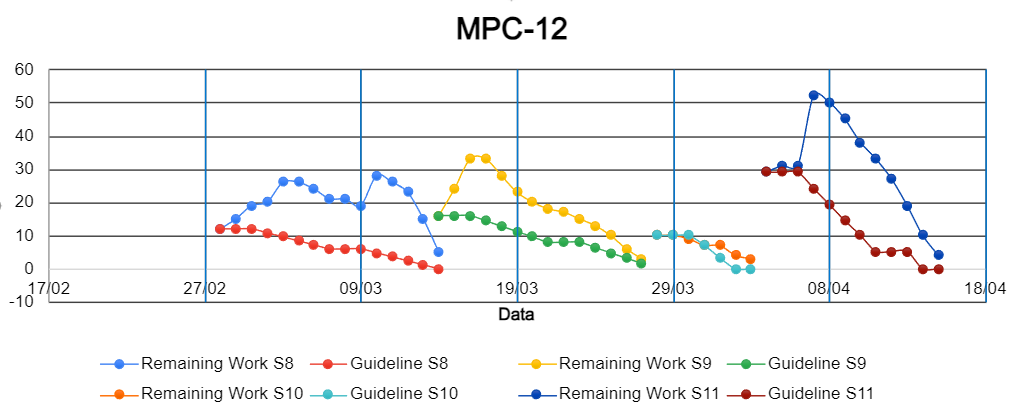
\includegraphics[width=\textwidth]{../../assets/pdq/burndown.png}
    \caption{MPC-12: Burndown Chart}
    \label{bc-burndown}
\end{figure}
\paragraph{PB - Product Baseline}
Il Burndown Chart mostra quanti work item sono ancora da svolgere all'interno di uno sprint, e qual'è l'andamento ideale per completare tutto il lavoro dello sprint. Nel nostro caso individuiamo un aumento delle attività da fare che coincide con la riunione interna di metà sprint, nella quale vengono solitamente aggiunte nuove task. Questo è molto visibile nello sprint 8.
\\ A partire dallo sprint 10 la durata degli sprint è stata ridotta a 1 settimana. È facilmente osservabile come il gruppo abbia seguito un andamento molto vicino a quello descritto dalla linea ideale descritta da Jira.\\
Quest'ultima infatti è una retta definita a tratti che va dal numero di work item all'inizio dello sprint a 0 alla fine dello sprint, senza considerare il weekend com giorni lavorativi. Il gruppo come descritto nelle norme di progetto si dava un margine per il caricamento delle task su Jira. Questo spiega la crescita del numero di work item nelle prime fasi degli sprint.

Può essere quindi generato un grafico che rapporti la quantità di lavoro svolta con quella pianificata, mostrando un andamento sia molto vicino o superiore a quello ideale.\\
Si può inoltre notare che con il passaggio a sprint più brevi lo svolgimento delle attività ha seguito uno sviluppo più vicino a quello ideale.
\begin{figure}[H]
    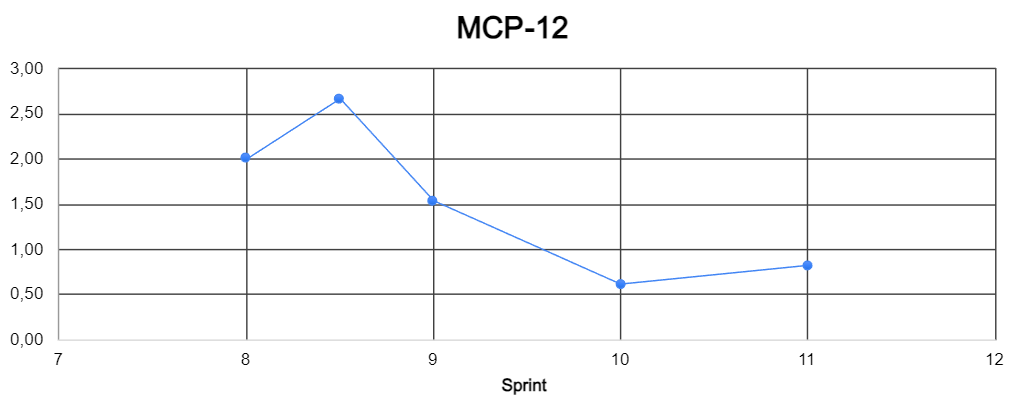
\includegraphics[width=\textwidth]{../../assets/pdq/burndown2.png}
    \caption{MPC-12: Burndown Chart Adherence}
    \label{bc-burndown-adherence}
\end{figure}

\subsection{MPC-13: Indice di Gulpease}
\begin{figure}[H]
    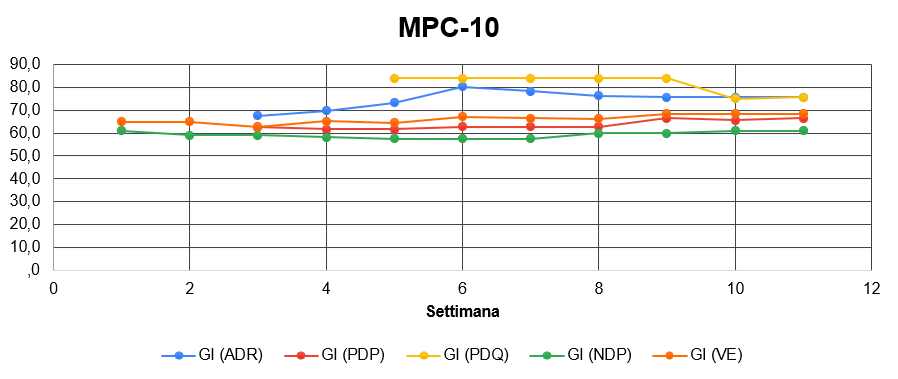
\includegraphics[width=\textwidth]{../../assets/pdq/gfi.png}
    \caption{MPC-13: Indice di Gulpease}
    \label{gfi}
\end{figure}
\paragraph{RTB - Requirements And Technology Baseline}
Il gruppo misura l'Indice di Gulpease per garantire la leggibilità, soprattutto
dei documenti rivolti ad esterni. Nelle fasi iniziali non è stata posta particolare
attenzione, ma i risultati sono stati comunque buoni. Un'eccezione sono le
Norme di Progetto: più descrittive e con pochi elenchi, mostrano valori inferiori.
Per garantire un limite minimo, nelle settimane 7--10 (SPRINT 4) è stato introdotto
un controllo automatico che accetta in repository solo documenti con Gulpease $\geq$ 60.
\paragraph{PB - Product Baseline}
L'andamento dei documenti già presenti è rimasto relativamente stabile. Per quanto riguarda i nuovi documenti, in particolare il Manuale Utente, è stata posta particolare attenzione. Tale documento per scopo, deve essere esposto a utenti non tecnici, e dunque è stato necessario garantire un indice di Gulpease elevato. Il gruppo ha quindi migliorato man mano la leggibilità del documento per garantire all'utente finale un'esperienza di lettura fluida e comprensibile.

\subsection{MPC-14: Correttezza ortografica}
\begin{figure}[H]
    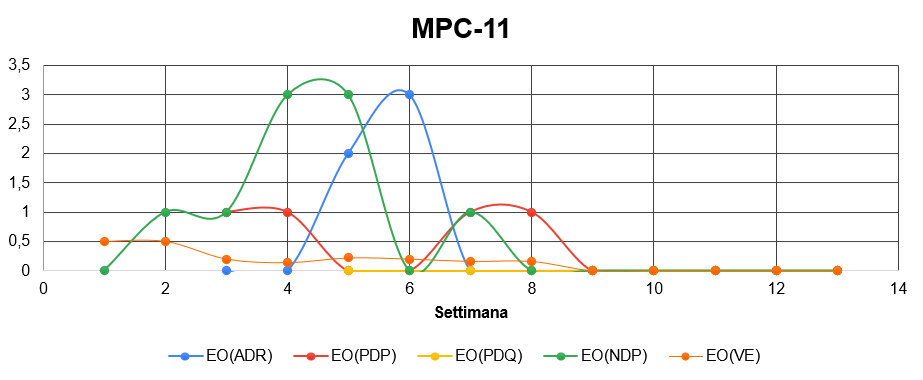
\includegraphics[width=\textwidth]{../../assets/pdq/eo.png}
    \caption{MPC-14: Correttezza ortografica}
    \label{eo}
\end{figure}
\paragraph{RTB - Requirements And Technology Baseline}
Gli errori ortografici sono stati gestiti in maniera analoga e parallela al Gulpease Index. Il gruppo ha deciso di non accettare documenti con errori ortografici, implementando un controllo automatico. Si osserva infatti come al termine della nona settimana i documenti risultano corretti.\\
\paragraph{PB - Product Baseline}
Similmente, anche nella seconda parte del progetto si è mantenuta l'attenzione su questo aspetto, controllando automaticamente che i documenti non presentassero errori ortografici e arrivando a una correttezza completa nelle ultime settimane di lavoro.\\

\subsection{MPC-16: Test success rate}
\begin{figure}[H]
    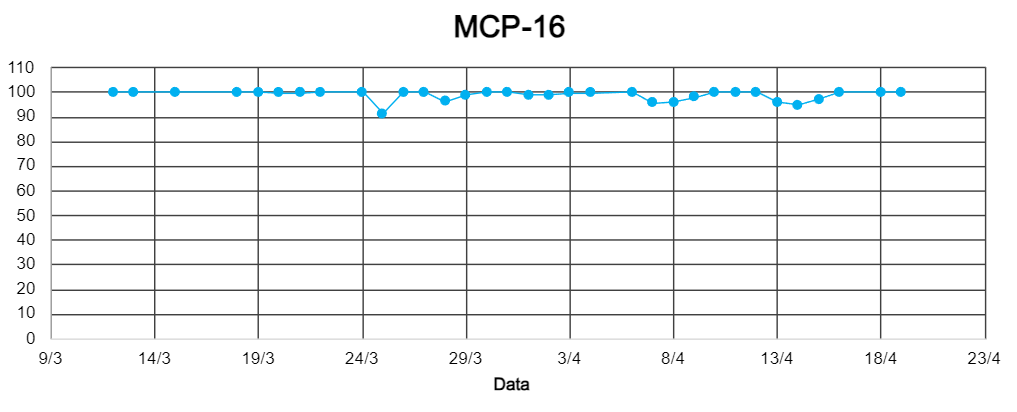
\includegraphics[width=\textwidth]{../../assets/pdq/passing_test.png}
    \caption{MPC-16: Test success rate}
    \label{tsr}
\end{figure}
\paragraph{PB - Product Baseline}
Il Test Success Rate mostra la percentuale di test superati rispetto al totale di test eseguiti. Il gruppo ha mantenuto un tasso che nella maggior parte dei casi è 100\%. I cali di questa metrica sono da attribuire ai merge dei diversi moduli che hanno introdotto bug.

\subsection{MPC-18: Rischi non previsti}
\begin{figure}[H]
    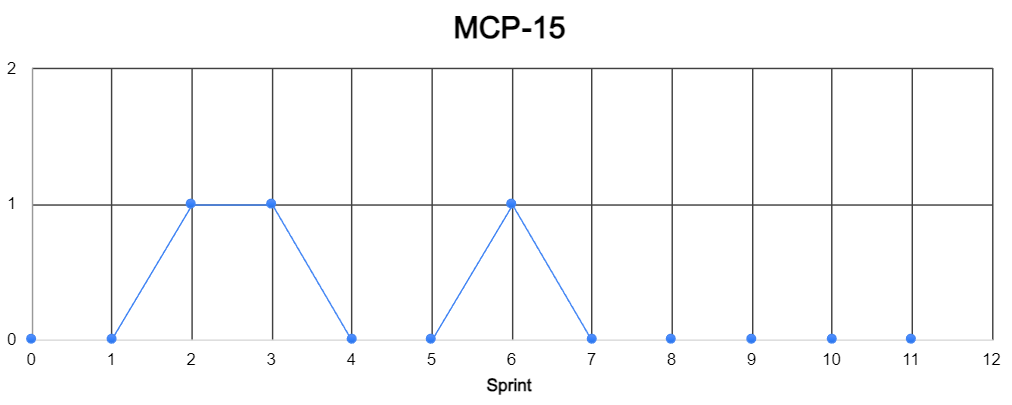
\includegraphics[width=\textwidth]{../../assets/pdq/rischi_imprevisti.png}
    \caption{MPC-18: Rischi non previsti}
    \label{rnp}
\end{figure}
\paragraph{RTB}
Il gruppo ha registrato due rischi imprevisti in due Sprint diversi. Il primo, coerente con i dati mostrati, è stato causato dalla sottostima delle attività.
Nel secondo Sprint si è verificato un rischio imprevedibile: un membro del gruppo è stato indisposto. Nello sprint 6 invece è stato riscontrato, coerentemente con quanto descritto in §\ref{crsc_ev_pv_ac}, uno sforamento dei costi inatteso. \\
\paragraph{PB - Product Baseline}
Per gli sprint successivi sono stati registrati rischi che però erano stati previsti all'inizio delle attività. Questo denota una migliore capacità di previsione, prevenendo l'insorgere di rischi guardando al passato e alle lezioni apprese.\\


\subsection{MPC-19: Metriche soddisfatte}
\begin{figure}[H]
    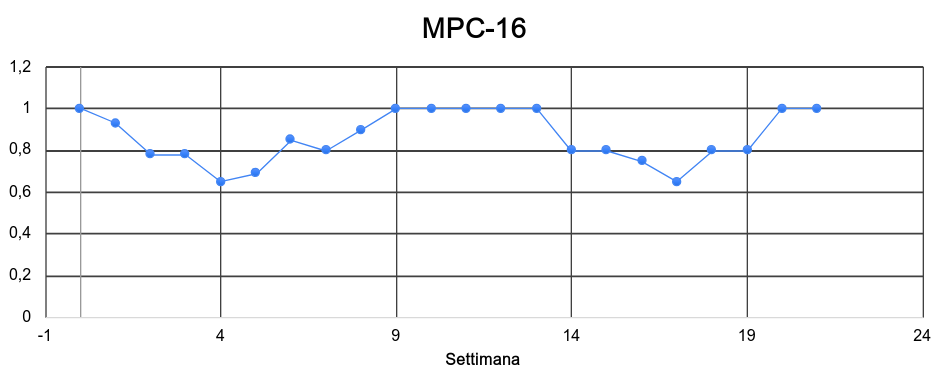
\includegraphics[width=\textwidth]{../../assets/pdq/ms.png}
    \caption{MPC-19: Metriche soddisfatte}
    \label{ms}
\end{figure}
\paragraph{RTB}
Si nota un calo iniziale, corrispondentemente al periodo di instabilità generale del progetto. Successivamente, grazie a misure correttive e ai controlli automatici di alcune metriche si è raggiunta la stabilità. Questo anche grazie alla crescente attenzione rivolta al soddisfacimento delle metriche di qualità.\\
\paragraph{PB - Product Baseline}
Similmente, si osserva una diminuizione in corrispondenza dell'inserimento di nuove metriche, che però è stata rapidamente recuperata, come nel primo periodo.\\

\subsection{MPD-1, MPD-2, MPD-3: Requisiti obbligatori, opzionali, desiderabili soddisfatti}

\begin{figure}[H]
    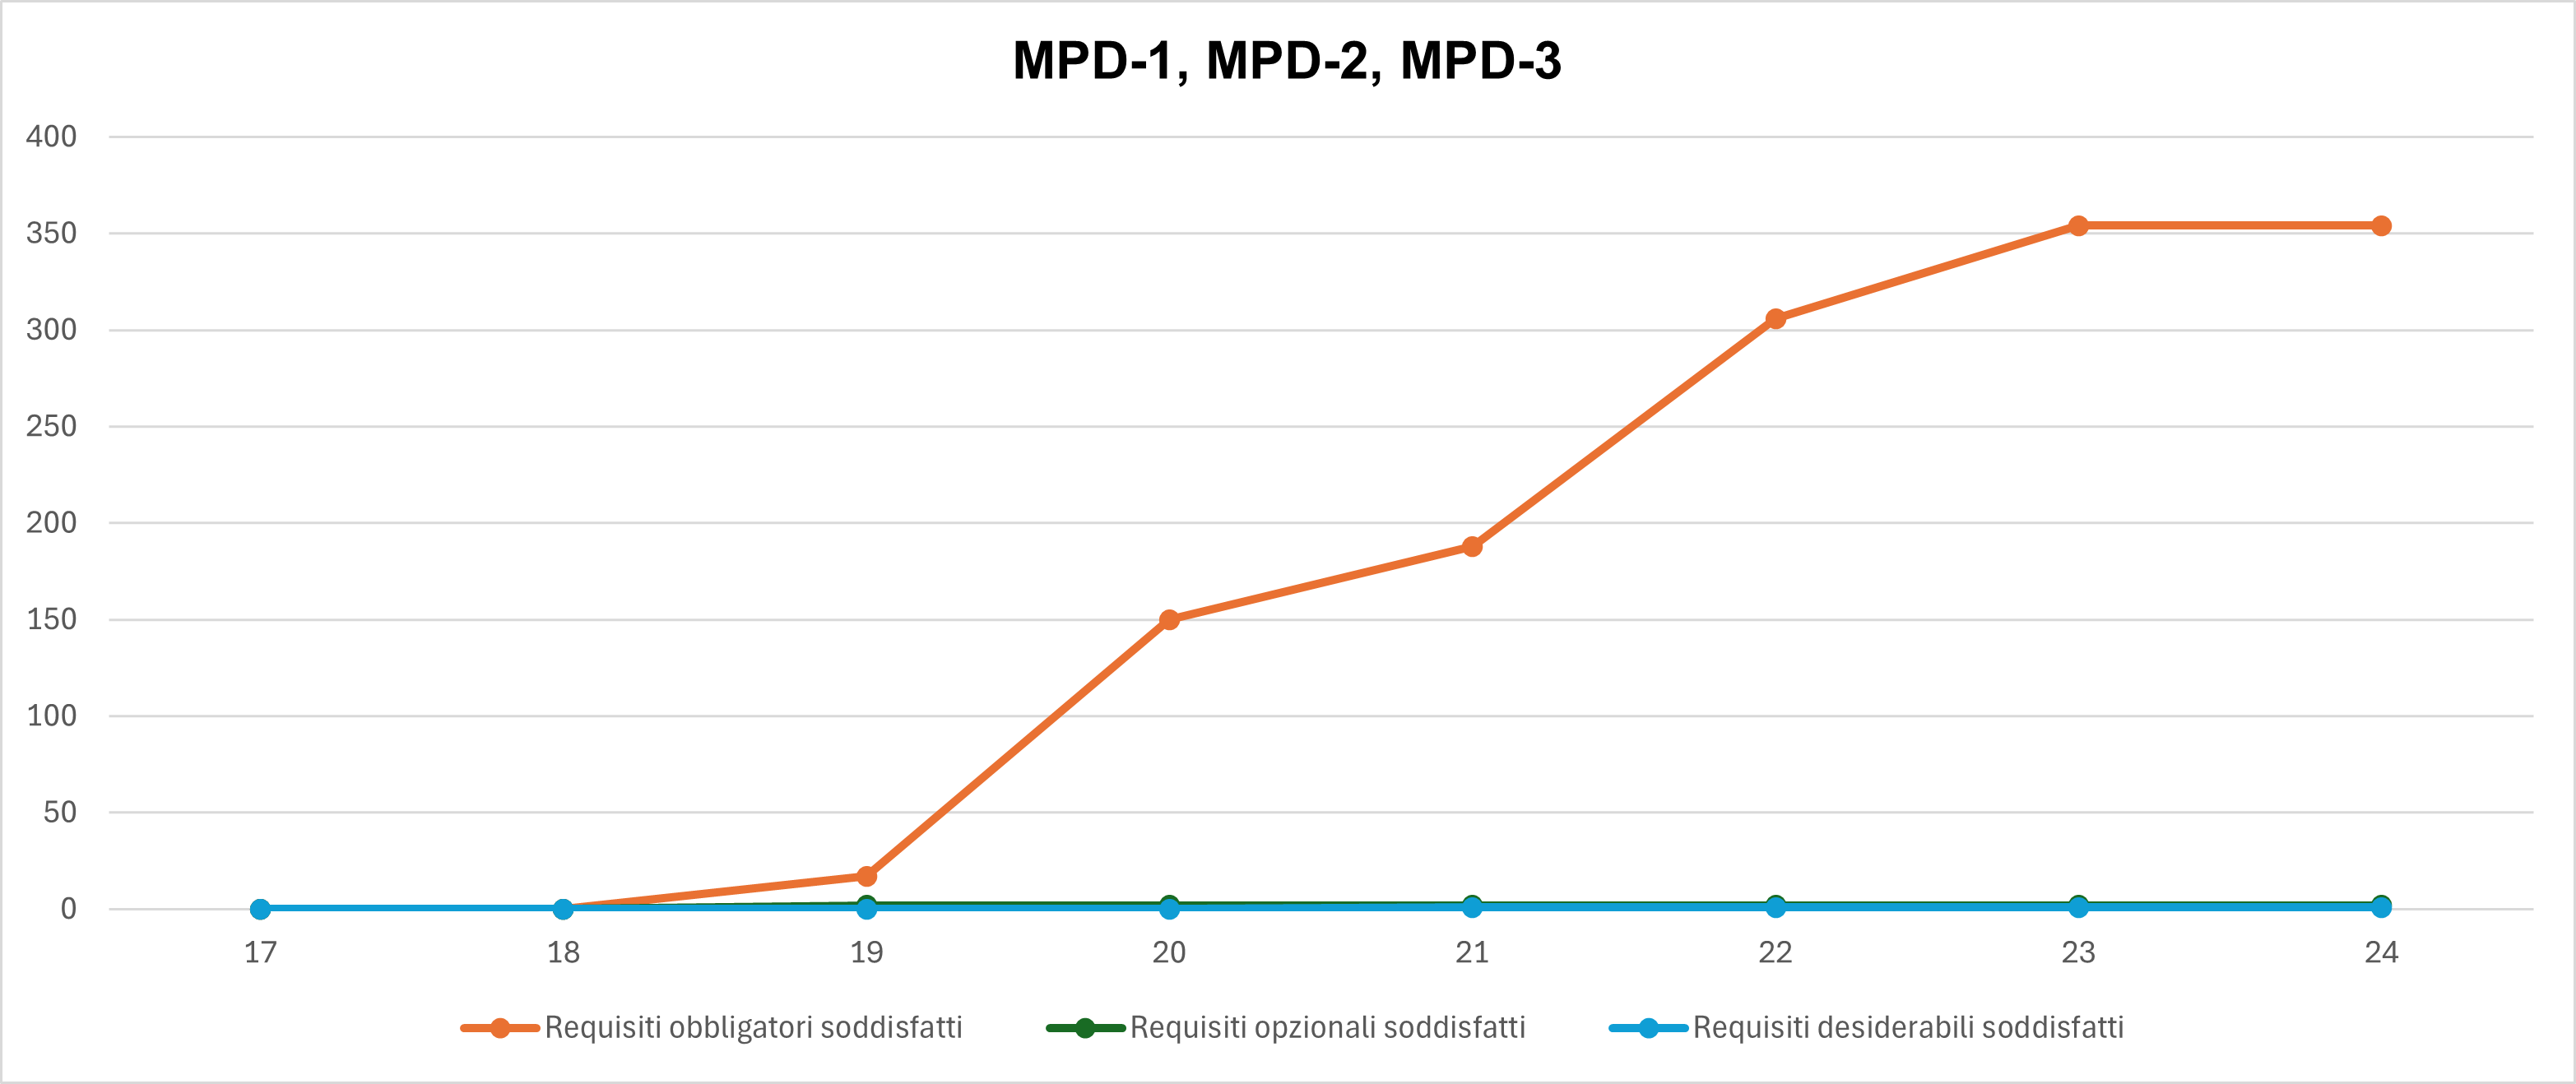
\includegraphics[width=\textwidth]{../../assets/pdq/MPD-1-2-3.png}
    \caption{MPD-1, MPD-2, MPD-3: Requisiti obbligatori, opzionali, desiderabili soddisfatti}
    \label{mpd-1-2-3}
\end{figure}
Il gruppo ha soddisfatto tutti i requisiti obbligatori. La maggior parte dei requisiti opzionali non sono stati soddisfatti, principalmente a causa di limitazioni di tempo e in parte anche per la complessità della funzionalità opzionale che riguardava quei requisiti. Per quanto riguarda l'unico requisito desiderabile, è stato soddisfatto.\\

\subsection{MPD-4: Broken Links}
\begin{figure}[H]
    \includegraphics[width=\textwidth]{../../assets/pdq/mpd-4.png}
    \caption{MPD-4: Broken Links}
    \label{mpd-4}
\end{figure}
\paragraph{PB - Product Baseline}
Nel contesto dell'applicazione i link rotti rappresentano collegamenti ai diversi componenti del layer frontend non funzionanti. Nel momento di picco di sviluppo la metrica è aumentata poiché il gruppo stava implementando le diverse funzionalità in maniera asincrona, senza preoccuparsi di collegare immediatamente i componenti. Successivamente, con l'avanzamento del progetto e la stabilizzazione del codice, il numero di link rotti è diminuito fino a raggiungere zero.\\

\subsection{MPD-5: Branch Coverage}
\begin{figure}[H]
    \includegraphics[width=\textwidth]{../../assets/pdq/mpd-5.png}
    \caption{MPD-5: Branch Coverage}
    \label{mpd-5}
\end{figure}
\paragraph{PB - Product Baseline}
La coverage è rimasta stabile sopra all'80\% per quasi ogni branch di sviluppo, con alcune eccezioni che si avvicinano comunque molto a questo valore. Si può notare che la misurazione della metrica ha permesso di rilevare e correggere le carenze dei branch di Navigazione e Import, confermando l'importanza di monitorare costantemente la qualità del codice.\\

\subsection{MPD-6: Statement Coverage}
\begin{figure}[H]
    \includegraphics[width=\textwidth]{../../assets/pdq/mpd-6.png}
    \caption{MPD-6: Statement Coverage}
    \label{mpd-6}
\end{figure}
\paragraph{PB - Product Baseline}
Lo statement coverage è rimasto stabilmente sopra all'80\% nei periodi finali grazie all'implementazione dei test in concomitanza con lo sviluppo del codice, senza delegare la scrittura dei test a fasi successive. Questo approccio è un'alternativa al test-driven development, che il gruppo ha ritenuto troppo rigido e limitante in fase di sviluppo iniziale in cui è stato necessario esplorare diversi approcci per implementare le funzionalità.\\

\subsection{MPD-7: Profondità di navigazione}
\begin{figure}[H]
    \includegraphics[width=\textwidth]{../../assets/pdq/mpd-7.png}
    \caption{MPD-7: Profondità di navigazione}
    \label{mpd-7}
\end{figure}
\paragraph{PB - Product Baseline}
La metrica di profondità di navigazione è indicatore diretto dell'usabilità del prodotto. Tenendo considerazione di questo aspetto, l'interfaccia utente prevede la massima profondità di navigazione nell'albero del DIP, che richiede al massimo 5 click per raggiungere qualsiasi elemento. Avendo definito questa profondità massima, la metrica è rimasta stabile durante tutto il progetto.\\

\subsection{MPD-8: Indexing Time}
\begin{figure}[H]
    \includegraphics[width=\textwidth]{../../assets/pdq/mpd-8.png}
    \caption{MPD-8: Indexing Time}
    \label{mpd-8}
\end{figure}
\paragraph{PB}
La metrica di indexing time è stata monitorata utilizzando lo stesso pacchetto DIP di test di dimensione 5GB. Nelle prime fasi di sviluppo l'indicizzazione era ancora ereditata dal POC, e dunque non ottimizzata. Con l'avanzamento del progetto e l'implementazione di un sistema di indicizzazione più efficiente, il tempo di indicizzazione è diminuito significativamente, per poi calare ulteriormente con il refactoring e l'unione delle transazioni in una unica verso il database SQLite.\\

\subsection{MPD-9: Search Time}
\begin{figure}[H]
    \includegraphics[width=\textwidth]{../../assets/pdq/mpd-9.png}
    \caption{MPD-9: Search Time}
    \label{mpd-9}
\end{figure}
\paragraph{PB - Product Baseline}
La metrica di search time è stata monitorata utilizzando lo stesso pacchetto DIP di test di dimensione 5GB. Nelle prime fasi di sviluppo il tempo di ricerca era ancora ereditato dal POC. Con il refactoring del database SQLite e l'ottimizzazione delle query, il tempo di ricerca è diminuito significativamente.

\subsection{MPD-10: Average CPU Usage}
\begin{figure}[H]
    \includegraphics[width=\textwidth]{../../assets/pdq/mpd-10.png}
    \caption{MPD-10: Average CPU Usage}
    \label{mpd-10}
\end{figure}
\paragraph{PB - Product Baseline}
L'utilizzo di CPU si è rivelato irrisorio fin da subito, il gruppo ha comunque mantenuto l'attenzione su questa metrica per evitare l'introduzione di bug che potessero causarne un aumento che sarebbe rimasto irrisolto.

\subsection{MPD-11: Peak Memory Usage}
\begin{figure}[H]
    \includegraphics[width=\textwidth]{../../assets/pdq/mpd-11.png}
    \caption{MPD-11: Peak Memory Usage}
    \label{mpd-11}
\end{figure}
\paragraph{PB - Product Baseline}
L'utilizzo di memoria è rimasto in larga parte vincolato dalla distribuzione Electron dell'applicazione, che prevede un limite inferiore di 300/400MB. Durante lo sviluppo la metrica è variata in maniera contenuta, senza mostrare criticità anche in situazioni di stress.\\


\subsection{MPD-12: Complessità ciclomatica}
\begin{figure}[H]
    \includegraphics[width=\textwidth]{../../assets/pdq/mpd-12-1.png}
    \caption{MPD-12: Complessità ciclomatica Frontend}
    \label{mpd-12-frontend}
\end{figure}
\begin{figure}[H]
    \includegraphics[width=\textwidth]{../../assets/pdq/mpd-12-2.png}
    \caption{MPD-12: Complessità ciclomatica Backend}
    \label{mpd-12-backend}
\end{figure}
\paragraph{PB - Product Baseline}
Il gruppo ha deciso di monitorare la complessità ciclomatica suddivisa per funzionalità di frontend e backend, in modo da fornire un quadro dettagliato e significativo pur rimanendo comprensibile e fruibile senza riportare la complessità per singolo file. Nel complesso il gruppo è riuscito a rispettare la soglia desiderabile di 15. Le eccezioni che si possono notare lato Backend sono risultato della presenza di poche specifiche funzioni che per natura richiedono un numero elevato di branch e non rappresentano un allarme per la qualità del codice. 

\subsection{MPD-13: Accoppiamento tra classi}
\begin{figure}[H]
    \includegraphics[width=\textwidth]{../../assets/pdq/mpd-13.png}
    \caption{MPD-13: Accoppiamento tra classi}
    \label{mpd-13}
\end{figure}
\paragraph{PB - Product Baseline}
L'accoppiamento tra classi è rimasto stabile durante tutto il progetto per via della progettazione iniziale che ha previsto un design destinato a non mutare, con un numero di dipendenze per classe che si è mantenuto al di sotto della soglia desiderabile di 5. 

\subsection{MPD-14: Code Smells}
\begin{figure}[H]
    \includegraphics[width=\textwidth]{../../assets/pdq/mpd-14.png}
    \caption{MPD-14: Code Smells}
    \label{mpd-14}
\end{figure}
\paragraph{PB - Product Baseline}
Lo strumento SonarQube ha permesso di monitorare code smells e di intervenire per correggerli. Gli avvisi significativi sono stati risolti tempestivamente, mentre altri che non rappresentavano un rischio per la qualità del codice ma semplicemente consigli di nomenclatura o di stile sono stati ignorati per ottimizzare il tempo a disposizione.\\

\subsection{MPD-15: Sistemi Operativi supportati}
\begin{figure}[H]
    \includegraphics[width=\textwidth]{../../assets/pdq/mpd-15.png}
    \caption{MPD-15: Sistemi Operativi supportati}
    \label{mpd-15}
\end{figure}
\paragraph{PB - Product Baseline}
Lo sviluppo si è svolto maggiormente su sistemi operativi Windows e Linux, con integrazione finale delle dipendenze necessarie per la build funzionante anche su macOS. La compatibilità finale quindi è stata raggiunta e verificata per tutti e tre i sistemi operativi principali.\\

\section{Strategie di testing}

\subsection{Test di accettazione}


\renewcommand{\arraystretch}{1.2}
\rowcolors{2}{gray!15}{white}
\begin{table}[H]
\centering
\small
\begin{tabular}{|p{1.5cm}|p{8.5cm}|c|}
\hline
\rowcolor{zpusgreen!30}
\textbf{Codice} & \textbf{Descrizione} & \textbf{Stato} \\
\hline
TA-1 & Verificare che l'utente possa accedere al sistema e consultare i documenti al suo interno & S \\
\hline
TA-2 & Verificare che l'utente possa navigare tra le cartelle e i file del DIP in modo intuitivo & S \\
\hline
TA-3 & Verificare che l'utente possa visualizzare i dettagli di una cartella selezionata & S \\
\hline
TA-4 & Verificare che l'utente possa selezionare uno o più file per poterli stampare o salvare & S \\
\hline
TA-5 & Verificare che l'utente possa visualizzare un'anteprima di un file selezionato & S \\
\hline
TA-6 & Verificare che l'utente possa verificare l'autenticità e l'integrità di un elemento & S \\
\hline
TA-7 & Verificare che l'utente possa visualizzare il contenuto di un elemento selezionato & S \\
\hline
TA-8 & Verificare che l'utente possa ricercare un file all'interno del DIP & S \\
\hline
TA-9 & Verificare che l'utente possa salvare uno o più file selezionati nel proprio dispositivo & S \\
\hline
TA-10 & Verificare che l'utente possa stampare uno o più file selezionati & S \\
\hline
TA-11 & Verificare che l'utente possa filtrare la ricerca degli elementi del DIP per attributi specifici & S \\
\hline
TA-12 & Verificare che l'utente possa effettuare una ricerca semantica basata su parole chiave e metadati degli elementi del DIP & S \\
\hline
\end{tabular}
\caption{Test di accettazione}
\label{tab:test-accettazione}
\end{table}

\subsection{Test di sistema}


\setlength{\LTleft}{-0.4cm}
\renewcommand{\arraystretch}{1.2}
\rowcolors{2}{gray!15}{white}
\begin{longtable}{|p{1.5cm}|p{8.3cm}|p{2.4cm}|c|}
\hline
\rowcolor{zpusgreen!30}
\textbf{Codice} & \textbf{Descrizione} & \textbf{Fonti} & \textbf{Stato} \\
\hline
\endfirsthead
\rowcolor{zpusgreen!30}
\textbf{Codice} & \textbf{Descrizione} & \textbf{Fonti} & \textbf{Stato} \\
\hline
\endhead

TS-1 & Verificare che l'utente possa visualizzare l'elenco di classi documentali nel DIP & R-1-F-Ob & S \\
\hline
TS-2 & Verificare che in caso non vi siano classi documentali nel DIP, l'utente possa visualizzare un messaggio di errore & R-2-F-Ob & S \\
\hline
TS-3 & Verificare che quando viene selezionata una classe documentale, l'utente possa visualizzare ciascuna classe documentale all'interno dell'elenco & R-3-F-Ob & S \\
\hline
TS-4 & Verificare che l'utente possa visualizzare il nome della classe documentale & R-4-F-Ob & S \\
\hline
TS-5 & Verificare che l'utente possa visualizzare lo stato di verifica della classe documentale & R-5-F-Ob & S \\
\hline
TS-6 & Verificare che l'utente possa visualizzare la marcatura temporale della classe documentale & R-6-F-Ob & S \\
\hline
TS-7 & Verificare che l'utente possa visualizzare l'elenco dei processi associati alla classe documentale & R-7-F-Ob & S \\
\hline
TS-8 & Verificare che in caso non vi siano processi associati alla classe documentale, l'utente possa visualizzare un messaggio di errore & R-8-F-Ob & S \\
\hline
TS-9 & Verificare che quando viene selezionato un processo, l'utente possa visualizzare ciascun processo all'interno dell'elenco & R-9-F-Ob & S \\
\hline
TS-10 & Verificare che l'utente possa visualizzare il nome del processo & R-10-F-Ob & S \\
\hline
TS-11 & Verificare che l'utente possa visualizzare l'elenco di documenti associati a un processo & R-12-F-Ob & S \\
\hline
TS-12 & Verificare che in caso non vi siano documenti associati al processo, l'utente possa visualizzare un messaggio di errore & R-13-F-Ob & S \\
\hline
TS-13 & Verificare che quando viene selezionato un documento, l'utente possa visualizzare ciascun documento all'interno dell'elenco & R-14-F-Ob & S \\
\hline
TS-14 & Verificare che l'utente possa visualizzare il nome del documento & R-15-F-Ob & S \\
\hline
TS-15 & Verificare che l'utente possa visualizzare lo stato di verifica del documento & R-16-F-Ob & S \\
\hline
TS-16 & Verificare che l'utente possa visualizzare la marcatura temporale del documento & R-17-F-Ob & S \\
\hline
TS-17 & Verificare che l'utente possa essere informato se un elenco di elementi del DIP risulta vuoto & R-18-F-Ob & S \\
\hline
TS-18 & L'utente deve poter visualizzare se il risultato dello stato di verifica di un elemento è "Non valido" & R-18-F-Ob & S \\
\hline
TS-19 & L'utente deve poter visualizzare se il risultato dello stato di verifica din elemento è "Valido" & R-19-F-Ob & S \\ 
\hline
TS-20 & L'utente deve poter visualizzare se il risultato dello stato di verifica di un elemento è "Non verificato" & R-20-F-Ob & S \\
\hline
TS-21 & Verificare che l'utente possa visualizzare l'anteprima di un documento selezionato & R-21-F-Ob & S \\
\hline
TS-22 & Verificare che se il documento selezionato non è visualizzabile in anteprima, l'utente possa visualizzare un messaggio di errore & R-22-F-Ob & S \\
\hline
TS-23 & Verificare che l'utente possa ricercare un documento, un processo, o una classe documentale & R-23-F-Ob & S \\
\hline
TS-24 & Verificare che l'utente possa cercare una classe documentale esclusivamente per nome & R-24-F-Ob & S \\
\hline
TS-25 & Verificare che l'utente possa effettuare una ricerca semantica basata sui metadati dei documenti presenti nel DIP & R-25-F-Op & S \\
\hline
TS-26 & Verificare che l'utente possa visualizzare lo stato dell'indicizzazione semantica & R-26-F-Op & NI \\
\hline
TS-27 & Verificare che l'utente possa visualizzare lo stato di indicizzazione semantica "Non completata" & R-27-F-Op & NI \\
\hline
TS-28 & Verificare che l'utente possa visualizzare lo stato di indicizzazione semantica "Completata" & R-28-F-Op & NI \\
\hline
TS-29 & Verificare che il sistema renda disponibile un campo di ricerca & R-29-F-Ob & S \\
\hline
TS-30 & Verificare che il sistema comunichi all'utente quando inserisce un valore non valido nel campo di ricerca & R-30-F-Ob & S \\
\hline
TS-31 & Verificare che il sistema renda disponibile l'opzione di ricerca per documenti & R-31-F-Ob & S \\
\hline
TS-32 & Verificare che il sistema renda disponibile l'opzione di ricerca per processi & R-32-F-Ob & S \\
\hline
TS-33 & Verificare che l'utente possa cercare un processo esclusivamente per uuid & R-33-F-Ob & S \\
\hline
TS-34 & Verificare che il sistema renda disponibile l'opzione di ricerca per classi documentali & R-34-F-Ob & S \\
\hline
TS-35 & Verificare che il sistema renda disponibile la ricerca avanzata con filtri & R-35-F-Ob & S \\
\hline
TS-36 & Verificare che il sistema renda disponibile la sezione di filtri di ricerca comuni & R-36-F-Ob & S \\
\hline
TS-37 & Verificare che il sistema renda disponibile la sezione di filtri di ricerca specifici per tipo documentale & R-37-F-Ob & S \\
\hline
TS-38 & Verificare che il sistema renda disponibile la sezione di filtri di ricerca specifici per metadati custom & R-38-F-Ob & S \\
\hline
TS-39 & Verificare che il sistema permetta di applicare più filtri contemporaneamente & R-39-F-Ob & S \\
\hline
TS-40 & Verificare che il sistema permetta di rimuovere i filtri applicati & R-40-F-Ob & S \\
\hline
TS-41 & Verificare che il sistema permetta di rimuovere tutti i filtri applicati & R-41-F-Ob & S \\
\hline
TS-42 & Verificare che il sistema permetta di selezionare filtri per tipo documentale per un singolo tipo di documento & R-42-F-Ob & S \\
\hline
TS-43 & Verificare che il sistema permetta di specificare il valore per i filtri per tipo Documento Informatico e Amministrativo Informatico & R-43-F-Ob & S \\
\hline
TS-44 & Verificare che il sistema racchiuda i filtri di ricerca comuni in una sezione espandibile dedicata & R-44-F-Ob & S \\
\hline
TS-45 & Verificare che il sistema racchiuda i filtri di ricerca specifici per tipo documentale in una sezione espandibile dedicata & R-45-F-Ob & S \\
\hline
TS-46 & Verificare che il sistema racchiuda i filtri di ricerca specifici per metadati custom in una sezione espandibile dedicata & R-46-F-Ob & S \\
\hline
TS-47 & Verificare che il sistema permetta di visualizzare i filtri comuni applicabili & R-47-F-Ob & S \\
\hline
TS-48 & Verificare che il sistema permetta di selezionare per la compilazione e l'aggiunta alla ricerca i filtri comuni & R-48-F-Ob & S \\
\hline
TS-49 & Verificare che il sistema renda disponibile una sezione per il filtro comune "Chiave Descrittiva" & R-49-F-Ob & S \\
\hline
TS-50 & Verificare che l'utente possa inserire il valore per il campo "Oggetto" & R-50-F-Ob & S \\
\hline
TS-51 & Verificare che l'utente possa inserire il valore per il campo "Parole chiave" & R-51-F-Ob & S \\
\hline
TS-52 & Verificare che il sistema renda disponibile una sezione per il filtro comune "Classificazione" & R-52-F-Ob & S \\
\hline
TS-53 & Verificare che l'utente possa inserire il valore per il campo "Indice di classificazione" & R-53-F-Ob & S \\
\hline
TS-54 & Verificare che l'utente possa inserire il valore per il campo "Descrizione" & R-54-F-Ob & S \\
\hline
TS-55 & Verificare che l'utente possa inserire il valore per il campo "Piano di classificazione" & R-55-F-Ob & S \\
\hline
TS-56 & Verificare che il sistema renda disponibile una sezione per il filtro comune "Tempo di conservazione" & R-56-F-Ob & S \\
\hline
TS-57 & Verificare che l'utente possa inserire il valore per il filtro "Tempo di conservazione" & R-57-F-Ob & S \\
\hline
TS-58 & Verificare che l'utente possa selezionare l'opzione "Perenne" per il filtro "Tempo di conservazione" & R-58-F-Ob & S \\
\hline
TS-59 & Verificare che il sistema renda disponibile una sezione per il filtro comune "Note" & R-59-F-Ob & S \\
\hline
TS-60 & Verificare che l'utente possa inserire il valore per il filtro "Note" & R-60-F-Ob & S \\
\hline
TS-61 & Verificare che il sistema renda disponibile una sezione per il filtro comune "Tipo di documento" & R-61-F-Ob & S \\
\hline
TS-62 & Verificare che l'utente possa selezionare il valore per il filtro "Tipo di documento" per il filtro "Documento informatico", "Documento amministrativo informatico", "Aggregazione documentale" & R-62-F-Ob & S \\
\hline
TS-63 & Verificare che l'utente possa selezionare il valore per il filtro "Tipo di documento" per il filtro "Documento amministrativo informatico" & R-63-F-Ob & S \\
\hline
TS-64 & Verificare che l'utente possa selezionare il valore per il filtro "Tipo di documento" per il filtro "Aggregazione documentale" & R-64-F-Ob & S \\
\hline
TS-65 & Verificare che il sistema renda disponibile una sezione per il filtro comune "Soggetto" & R-65-F-Ob & S \\
\hline
TS-66 & Verificare che l'utente possa inserire il valore per il filtro "Soggetto" & R-66-F-Ob & S \\
\hline
TS-67 & Verificare che il sistema renda disponibile una sezione per il filtro del Ruolo del Soggetto & R-67-F-Ob & S \\
\hline
TS-68 & Verificare che il sistema renda disponibile una sezione per il filtro del Tipo di Soggetto & R-68-F-Ob & S \\
\hline
TS-69 & Verificare che il sistema renda disponibile una sezione per il filtro "Dettagli" del Soggetto & R-69-F-Ob & S \\
\hline
TS-70 & Verificare che se il soggetto selezionato è di tipo "PAI", all'interno della sezione del filtro "Dettagli" del Soggetto, l'utente possa inserire il valore per i campi "Denominazione Amministrazione/Codice IPA", "Denominazione Amministrazione AOO/Codice IPA AOO", "Denominazione Amministrazione UOR/Codice IPA UOR" e "Indirizzi digitali di riferimento" & R-70-F-Ob & S \\
\hline
TS-71 & Verificare che l'utente possa inserire il valore per il campo "Denomizazione Amministrazione/Codice IPA" & R-71-F-Ob & S \\
\hline
TS-72 & Verificare che l'utente possa inserire il valore per il campo "Denominazione Amministrazione AOO/Codice IPA AOO" & R-72-F-Ob & S \\
\hline
TS-73 & Verificare che l'utente possa inserire il valore per il campo "Denominazione Amministrazione UOR/Codice IPA UOR" & R-73-F-Ob & S \\
\hline
TS-74 & Verificare che l'utente possa inserire il valore per il campo "Indirizzi digitali di riferimento" & R-74-F-Ob & S \\

\hline
TS-75 & Verificare che se il soggetto selezionato è di tipo "PAE", all'interno della sezione del filtro "Dettagli" del Soggetto, l'utente possa inserire il valore per i campi "Denominazione Amministrazione", "Denominazione Ufficio" e "Indirizzi digitali di riferimento" & R-75-F-Ob & S \\
\hline
TS-76 & Verificare che l'utente possa inserire il valore per il campo "Denominazione Amministrazione" & R-76-F-Ob & S \\
\hline
TS-77 & Verificare che l'utente possa inserire il valore per il campo "Denominazione Ufficio" & R-77-F-Ob & S \\
\hline
TS-78 & Verificare che se il soggetto selezionato è di tipo "AS", all'interno della sezione del filtro "Dettagli" del Soggetto, l'utente possa inserire il valore per i campi "Cognome", "Nome", "Codice Fiscale", "Denominazione Amministrazione AOO/Codice IPA AOO", "Denominazione Amministrazione UOR/Codice IPA UOR" e "Indirizzi digitali di riferimento" & R-78-F-Ob & S \\
\hline
TS-79 & Verificare che l'utente possa inserire il valore per il campo "Cognome" & R-79-F-Ob & S \\
\hline
TS-80 & Verificare che l'utente possa inserire il valore per il campo "Nome" & R-80-F-Ob & S \\
\hline
TS-81 & Verificare che l'utente possa inserire il valore per il campo "Codice Fiscale/Partita IVA" & R-81-F-Ob & S \\
\hline
TS-82 & Verificare che se il soggetto selezionato è di tipo "PG", all'interno della sezione del filtro "Dettagli" del Soggetto, l'utente possa inserire il valore per i campi "Denominazione Organizzazione", "Codice Fiscale/Partita IVA", "Denominazione Ufficio" e "Indirizzi digitali di riferimento" & R-82-F-Ob & S \\
\hline
TS-83 & Verificare che l'utente possa inserire il valore per il campo "Denominazione Organizzazione" & R-83-F-Ob & S \\
\hline
TS-84 & Verificare che se il soggetto selezionato è di tipo "PF", all'interno della sezione del filtro "Dettagli" del Soggetto, l'utente possa inserire il valore per i campi "Cognome", "Nome" e "Indirizzi digitali di riferimento" & R-84-F-Ob & S \\
\hline
TS-85 & Verificare che se il soggetto selezionato è di tipo "RUP", all'interno della sezione del filtro "Dettagli" del Soggetto, l'utente possa inserire il valore per i campi "Cognome", "Nome", "Codice Fiscale" "Denominazione Amministrazione/Codice IPA", "Denominazione Amministrazione AOO/Codice IPA AOO", "Denominazione Amministrazione UOR/Codice IPA UOR" e "Indirizzi digitali di riferimento" & R-85-F-Ob & S \\
\hline
TS-86 & Verificare che se il soggetto selezionato è di tipo "SW", all'interno della sezione del filtro "Dettagli" del Soggetto, l'utente possa inserire il valore per il campo "Denominazione Sistema" & R-86-F-Ob & S \\
\hline
TS-87 & Verificare che l'utente possa inserire il valore per il campo "Denominazione Sistema" & R-87-F-Ob & S \\
\hline
TS-88 & Verificare che all'interno di una ricerca con filtri, l'utente possa visualizzare il nome del campo in una lista & R-88-F-Ob & S \\
\hline
TS-89 & Verificare che all'interno della sezione di filtri per tipo documentale, il sistema permetta di selezionare i filtri specifici per il tipo "Documento Informatico e Amministrativo Informatico" & R-89-F-Ob & S \\
\hline
TS-90 & Verificare che per il Documento Informatico e Amministrativo Informatico, il sistema renda disponibile una sezione per il filtro "Dati di Registrazione" & R-90-F-Ob & S \\
\hline
TS-91 & Verificare che l'utente possa inserire il valore per il campo "Tipologia di flusso" & R-91-F-Ob & S \\
\hline
TS-92 & Verificare che l'utente possa specificare la tipologia "Entrata" per la tipologia di flusso & R-92-F-Ob & S \\
\hline
TS-93 & Verificare che l'utente possa specificare la tipologia "Uscita" per la tipologia di flusso & R-93-F-Ob & S \\
\hline
TS-94 & Verificare che l'utente possa specificare la tipologia "Interno" per la tipologia di flusso & R-94-F-Ob & S \\
\hline
TS-95 & Verificare che l'utente possa inserire il valore per il campo "Tipo di registro" & R-95-F-Ob & S \\
\hline
TS-96 & Verificare che l'utente possa specificare la tipologia "Nessuno" per il tipo di registro & R-96-F-Ob & S \\
\hline
TS-97 & Verificare che l'utente possa specificare la tipologia "Protocolo Ordinario/Protocollo Emergenza" per il tipo di registro & R-97-F-Ob & S \\
\hline
TS-98 & Verificare che l'utente possa specificare la tipologia "Repertorio/Registro" per il tipo di registro & R-98-F-Ob & S \\
\hline
TS-99 & Verificare che l'utente possa inserire il valore per il campo "Data di registrazione" & R-99-F-Ob & S \\
\hline
TS-100 & Verificare che l'utente possa inserire il valore per il campo "Numero documento" & R-100-F-Ob & S \\
\hline
TS-101 & Verificare che l'utente possa inserire il valore per il campo "Codice registro" & R-101-F-Ob & S \\
\hline
TS-102 & Verificare che per il Documento Informatico e Amministrativo Informatico, l'utente possa inserire il valore per il filtro "Tipologia Documentale" & R-102-F-Ob & S \\
\hline
TS-103 & Verificare che per il Documento Informatico e Amministrativo Informatico, l'utente possa inserire il valore per il filtro "Modalità di Formazione" & R-103-F-Ob & S \\
\hline
TS-104 & Verificare che l'utente possa specificare la modalità "Ex novo" per il filtro "Modalità di Formazione" & R-104-F-Ob & S \\
\hline
TS-105 & Verificare che l'utente possa specificare la modalità "Acquisizione da altro documento o supporto informatico" per il filtro "Modalità di Formazione" & R-105-F-Ob & S \\
\hline
TS-106 & Verificare che l'utente possa specificare la modalità "Memorizzazione su supporto informatico in formato digitale" per il filtro "Modalità di Formazione" & R-106-F-Ob & S \\
\hline
TS-107 & Verificare che l'utente possa specificare la modalità "Generazione o raggruppamento in forma statica" per il filtro "Modalità di Formazione" & R-107-F-Ob & S \\
\hline
TS-108 & Verificare che per il Documento Informatico e Amministrativo Informatico, l'utente possa inserire il valore per il filtro "Campo Riservato" tra "S" o "No" & R-108-F-Ob & S \\
\hline
TS-109 & Verificare che per il Documento Informatico e Amministrativo Informatico, il sistema renda disponibile una sezione per il filtro "Identificativo del Formato" & R-109-F-Ob & S \\
\hline
TS-110 & Verificare che l'utente possa inserire il valore per il campo "Formato" & R-110-F-Ob & S \\
\hline
TS-111 & Verificare che l'utente possa inserire il valore per il campo "Prodotto Software" & R-111-F-Ob & S \\
\hline
TS-112 & Verificare che l'utente possa inserire il valore per il campo "Versione Prodotto" & R-112-F-Ob & S \\
\hline
TS-113 & Verificare che l'utente possa inserire il valore per il campo "Produttore" & R-113-F-Ob & S \\
\hline
TS-114 & Verificare che per il Documento Informatico e Amministrativo Informatico, il sistema renda disponibile una sezione per il filtro "Dati di Verifica" & R-114-F-Ob & S \\
\hline
TS-115 & Verificare che l'utente possa inserire il valore per il campo "Firmato Digitalmente" tra "S" o "No" all'interno della sezione del filtro "Dati di Verifica" & R-115-F-Ob & S \\
\hline
TS-116 & Verificare che l'utente possa inserire il valore per il campo "Sigillato Elettronicamente" tra "S" o "No" all'interno della sezione del filtro "Dati di Verifica" & R-116-F-Ob & S \\
\hline
TS-117 & Verificare che l'utente possa inserire il valore per il campo "Marcatura Temporale" tra "S" o "No" all'interno della sezione del filtro "Dati di Verifica" & R-117-F-Ob & S \\
\hline
TS-118 & Verificare che l'utente possa inserire il valore per il campo "Conformità copie immagine su supporto informatico" tra "S" o "No" all'interno della sezione del filtro "Dati di Verifica" & R-118-F-Ob & S \\
\hline
TS-119 & Verificare che per il Documento Informatico e Amministrativo Informatico, l'utente possa inserire il valore per il filtro "Nome del Documento" & R-119-F-Ob & S \\
\hline
TS-120 & Verificare che per il Documento Informatico e Amministrativo Informatico, l'utente possa inserire il valore per il filtro "Versione del Documento" & R-120-F-Ob & S \\
\hline
TS-121 & Verificare che per il Documento Informatico e Amministrativo Informatico, l'utente possa inserire il valore per il filtro "Identificativo del Documento Primario" & R-121-F-Ob & S \\
\hline
TS-122 & Verificare che per il Documento Informatico e Amministrativo Informatico, il sistema renda disponibile una sezione per il filtro "Tracciatura Modifiche di Documento" & R-122-F-Ob & S \\
\hline
TS-123 & Verificare che l'utente possa inserire il valore per i campi "Tipo di Modifica" all'interno della sezione del filtro "Tracciatura Modifiche di Documento" & R-123-F-Ob & S \\
\hline
TS-124 & Verificare che l'utente possa specificare il valore "Annullamento" per il campo "Tipo di Modifica" & R-124-F-Ob & S \\
\hline
TS-125 & Verificare che l'utente possa specificare il valore "Rettifica" per il campo "Tipo di Modifica" & R-125-F-Ob & S \\
\hline
TS-126 & Verificare che l'utente possa specificare il valore "Integrazione" per il campo "Tipo di Modifica" & R-126-F-Ob & S \\
\hline
TS-127 & Verificare che l'utente possa specificare il valore "Annotazione" per il campo "Tipo di Modifica" & R-127-F-Ob & S \\
\hline
TS-128 & Verificare che l'utente possa inserire il valore per il campo "Data/Ora della Modifica" all'interno della sezione del filtro "Tracciatura Modifiche di Documento" & R-128-F-Ob & S \\
\hline
TS-129 & Verificare che l'utente possa inserire il valore per il campo "Identificativo Documento Versione Precedente" all'interno della sezione del filtro "Tracciatura Modifiche di Documento" & R-129-F-Ob & S \\
\hline
TS-130 & Verificare che all'interno della sezione di filtri per tipo documentale, il sistema permetta di selezionare i filtri specifici per il tipo "Aggregazione Documentale Informatica" & R-130-F-Ob & S \\
\hline
TS-131 & Verificare che per l'Aggregazione Documentale Informatica, il sistema renda disponibili per la compilazione e l'aggiunta alla ricerca i filtri specifici & R-131-F-Ob  & S \\
\hline
TS-132 & Verificare che per l'Aggregazione Documentale Informatica, il sistema renda disponibile una sezione per il filtro "Tipo di Aggregazione" & R-132-F-Ob & S \\
\hline
TS-133 & Verificare che l'utente possa inserire il valore "Fascicolo" per il filtro "Tipo di Aggregazione" & R-133-F-Ob & S \\
\hline
TS-134 & Verificare che l'utente possa inserire il valore "Serie Documentale" per il filtro "Tipo di Aggregazione" & R-134-F-Ob & S \\
\hline
TS-135 & Verificare che l'utente possa inserire il valore "Serie di fascicoli" per il filtro "Tipo di Aggregazione" & R-135-F-Ob & S \\
\hline
TS-136 & Verificare che per l'Aggregazione Documentale Informatica, l'utente possa inserire il valore per il filtro "Identificativo dell'Aggregazione Documentale" & R-136-F-Ob & S \\
\hline
TS-137 & Verificare che l'utente possa inserire il valore per il filtro "Tipologia di Fascicolo" & R-137-F-Ob & S \\
\hline
TS-138 & Verificare che l'utente possa specificare il valore "Affare" per il filtro "Tipologia di Fascicolo" & R-138-F-Ob & S \\
\hline
TS-139 & Verificare che l'utente possa specificare il valore "Attività" per il filtro "Tipologia di Fascicolo" & R-139-F-Ob & S \\
\hline
TS-140 & Verificare che l'utente possa specificare il valore "Persona Fisica" per il filtro "Tipologia di Fascicolo" & R-140-F-Ob & S \\
\hline
TS-141 & Verificare che l'utente possa specificare il valore "Persona Giuridica" per il filtro "Tipologia di Fascicolo" & R-141-F-Ob & S \\
\hline
TS-142 & Verificare che l'utente possa specificare il valore "Procedimento Amministrativo" per il filtro "Tipologia di Fascicolo" & R-142-F-Ob & S \\
\hline
TS-143 & Verificare che per l'Aggregazione Documentale Informatica, l'utente possa inserire il valore per il filtro "Id Aggregazione Primario" & R-143-F-Ob & S \\
\hline
TS-144 & Verificare che per l'Aggregazione Documentale Informatica, l'utente possa inserire il valore per il filtro "Data Apertura" & R-144-F-Ob & S \\
\hline
TS-145 & Verificare che per l'Aggregazione Documentale Informatica, l'utente possa inserire il valore per il filtro "Data Chiusura" & R-145-F-Ob & S \\
\hline
TS-146 & Verificare che per l'Aggregazione Documentale Informatica, il sistema renda disponibile una sezione per il filtro "Procedimento Amministrativo" & R-146-F-Ob & S \\
\hline
TS-147 & Verificare che l'utente possa inserire il valore per il campo "Materia/Argomento/Struttura" & R-147-F-Ob & S \\
\hline
TS-148 & Verificare che l'utente possa inserire il valore per il campo "Procedimento" & R-148-F-Ob & S \\
\hline
TS-149 & Verificare che l'utente possa inserire il valore per il campo "Catalogo Procedimenti" & R-149-F-Ob & S \\
\hline
TS-150 & Verificare che per l'Aggregazione Documentale Informatica, il sistema renda disponibile una sezione per il filtro "Fasi" & R-150-F-Ob & S \\
\hline
TS-151 & Verificare che l'utente possa inserire il valore per il campo "Tipo Fase" all'interno della sezione del filtro "Fasi". & R-151-F-Ob & S \\
\hline
TS-152 & Verificare che l'utente possa specificare il valore "Preparatoria" per il campo "Tipo Fase" & R-152-F-Ob & S \\
\hline
TS-153 & Verificare che l'utente possa specificare il valore "Istruttoria" per il campo "Tipo Fase" & R-153-F-Ob & S \\
\hline
TS-154 & Verificare che l'utente possa specificare il valore "Consultiva" per il campo "Tipo Fase" & R-154-F-Ob & S \\
\hline
TS-155 & Verificare che l'utente possa specificare il valore "Decisoria" per il campo "Tipo Fase" & R-155-F-Ob & S \\
\hline
TS-156 & Verificare che l'utente possa specificare il valore "Integrazione dell'efficacia" per il campo "Tipo Fase" & R-156-F-Ob & S \\
\hline
TS-157 & Verificare che l'utente possa inserire il valore per il campo "Data Inizio Fase" all'interno della sezione del filtro "Fasi" & R-157-F-Ob & S \\
\hline
TS-158 & Verificare che l'utente possa inserire il valore per il campo "Data Fine Fase" all'interno della sezione del filtro "Fasi" & R-158-F-Ob & S \\
\hline
TS-159 & Verificare che per l'Aggregazione Documentale Informatica, il sistema renda disponibile una sezione per il filtro "Assegnazione" & R-159-F-Ob & S \\
\hline
TS-160 & Verificare che l'utente possa inserire il valore per il campo "Assegnazione" all'interno della sezione del filtro "Assegnazione" & R-160-F-Ob & S \\
\hline
TS-161 & Verificare che l'utente possa inserire il valore per il campo "Tipo Assegnazione" & R-161-F-Ob & S \\
\hline
TS-162 & Verificare che l'utente possa specificare il valore "Per competenza" per il campo "Tipo Assegnazione" & R-162-F-Ob & S \\
\hline
TS-163 & Verificare che l'utente possa specificare il valore "Per conoscenza" per il campo "Tipo Assegnazione" & R-163-F-Ob & S \\
\hline
TS-164 & Verificare che l'utente possa inserire il valore per il campo "Data Inizio Assegnazione" all'interno della sezione del filtro "Assegnazione" & R-164-F-Ob & S \\
\hline
TS-165 & Verificare che l'utente possa inserire il valore per il campo "Data Fine Assegnazione" all'interno della sezione del filtro "Assegnazione" & R-165-F-Ob & S \\
\hline
TS-166 & Verificare che per l'Aggregazione Documentale Informatica, l'utente possa inserire il valore per il filtro "Progressivo Aggregazione" & R-166-F-Ob & S \\
\hline
TS-167 & Verificare che all'interno della sezione di filtri per custom metadata, il sistema permetta di selezionare i filtri specifici per i metadata presenti & R-167-F-Ob & S \\
\hline
TS-168 & Verificare che per ciascun custom metadata, l'utente possa inserire il nome del metadato e il relativo valore & R-168-F-Ob & S \\
\hline
TS-169 & Verificare che quando viene eseguita una ricerca, l'utente possa visualizzare i risultati della ricerca & R-169-F-Ob & S \\
\hline
TS-170 & Verificare che l'utente possa visualizzare per ogni risultato le informazioni rilevanti: Nome del documento o aggregazione, Data di registrazione/creazione del documento/aggregazione, Tipo di elemento tra Documento, Aggregazione, Processo o Classe Documentale & R-170-F-Ob & S \\
\hline
TS-171 & Verificare che l'utente possa visualizzare il nome del documento o aggregazione & R-171-F-Ob & S \\
\hline
TS-172 & Verificare che l'utente possa visualizzare il tipo del documento o aggregazione & R-172-F-Ob & S \\
\hline
TS-173 & Verificare che se la ricerca non produce risultati, l'utente possa visualizzare un messaggio di errore & R-173-F-Ob & S \\
\hline
TS-174 & Verificare che il sistema prevenga l'inserimento di valori testuali non validi & R-174-F-Ob & S \\
\hline
TS-175 & Verificare che il sistema prevenga l'inserimento di valori numerici non validi & R-175-F-Ob & S \\
\hline
TS-176 & Verificare che il sistema informi l'utente quando il formato del valore data inserito non è valido & R-176-F-Ob & S \\
\hline
TS-177 & Verificare che il sistema informi l'utente quando il formato del valore numerico positivo inserito non è valido & R-177-F-Ob & S \\
\hline
TS-178 & Verificare che l'utente possa salvare un documento in locale in una cartella selezionata & R-178-F-Ob & S \\
\hline
TS-179 & Verificare che l'utente possa salvare più file documentali in una cartella selezionata & R-179-F-Ob & S \\
\hline
TS-180 & Verificare che se il salvataggio di uno o più documenti fallisce, l'utente possa visualizzare un messaggio di errore & R-180-F-Ob & S \\
\hline
TS-181 & Verificare che l'utente possa stampare un documento & R-181-F-Ob & S \\
\hline
TS-182 & Verificare che l'utente possa stampare un insieme di documenti & R-182-F-Op & NI \\
\hline
TS-183 & Verificare che se la stampa di uno o più documenti fallisce, l'utente possa visualizzare un messaggio di errore & R-183-F-Op & S \\
\hline
TS-184 & Verificare che se la stampa non è disponibile, l'utente possa visualizzare un messaggio di stampa non avvenuta & R-184-F-Ob & S \\
\hline
TS-185 & Verificare che l'utente possa avviare la verifica del DIP & R-185-F-Ob & S \\
\hline
TS-186 & Verificare che l'utente possa visualizzare lo stato di verifica del DIP & R-186-F-Ob & S \\
\hline
TS-187 & Verificare che l'utente possa avviare la verifica della classe documentale & R-187-F-Ob & S \\
\hline
TS-188 & Verificare che l'utente possa visualizzare lo stato di verifica della classe documentale & R-188-F-Ob & S \\
\hline
TS-189 & Verificare che l'utente possa avviare la verifica dell'integrità processo & R-189-F-Ob & S \\
\hline
TS-190 & Verificare che l'utente possa visualizzare lo stato di verifica dell'integrità processo & R-190-F-Ob & S \\
\hline
TS-191 & Verificare che l'utente possa avviare la verifica del documento & R-191-F-Ob & S \\
\hline
TS-192 & Verificare che l'utente possa visualizzare lo stato di verifica del documento & R-192-F-Ob & S \\
\hline
TS-193 & Verificare che l'utente possa visualizzare il report di integrità del DIP completo con le informazioni aggregate & R-193-F-Ob & S \\
\hline
TS-194 & Verificare che l'utente possa visualizzare il conteggio totale delle classi documentali verificate nel report del DIP & R-194-F-Ob & S \\
\hline
TS-195 & Verificare che l'utente possa visualizzare il numero di classi integre (stato "Valido") in colore verde nel report del DIP & R-195-F-Ob & S \\
\hline
TS-196 & Verificare che l'utente possa visualizzare il numero di classi corrotte (stato "Non Valido") in colore rosso nel report del DIP & R-196-F-Ob & S \\
\hline
TS-197 & Verificare che l'utente possa visualizzare l'elenco delle classi corrotte indicando nome e numero di processi corrotti per ciascuna & R-197-F-Ob & S \\
\hline
TS-198 & Verificare che l'utente possa visualizzare la classe corrotta indicando nome e numero di processi corrotti & R-198-F-Ob & S \\
\hline
TS-199 & Verificare che l'utente possa visualizzare la data e l'ora di inizio della verifica del DIP nel formato "GG/MM/AAAA HH:MM:SS" & R-199-F-Op & NI \\
\hline
TS-200 & Verificare che l'utente sia informato con un messaggio nel caso in cui non vi siano classi corrotte & R-200-F-Op & NI \\
\hline
TS-201 & Verificare che l'utente possa visualizzare il report di integrità dettagliato per una singola classe documentale & R-201-F-Op & NI \\
\hline
TS-202 & Verificare che l'utente possa visualizzare il conteggio dei processi verificati all'interno della classe documentale & R-202-F-Ob & S \\
\hline
TS-203 & Verificare che l'utente possa visualizzare il numero di processi integri (stato "Valido") in colore verde nella classe documentale & R-203-F-Ob & S \\
\hline
TS-204 & Verificare che l'utente possa visualizzare il numero di processi corrotti (stato "Non Valido") in colore rosso nella classe documentale & R-204-F-Ob & S \\
\hline
TS-205 & Verificare che l'utente possa visualizzare la lista dei processi corrotti con il relativo numero di documenti compromessi & R-205-F-Ob & S \\
\hline
TS-206 & Verificare che l'utente possa visualizzare il singolo processo corrotto con il relativo numero di documenti compromessi & R-206-F-Ob & S \\
\hline
TS-207 & Verificare che l'utente possa visualizzare la data e l'ora di inizio della verifica della classe nel formato "GG/MM/AAAA HH:MM:SS" & R-207-F-Op & NI \\
\hline
TS-208 & Verificare che l'utente sia informato che tutti i processi sono integri & R-208-F-Op & NI \\
\hline
TS-209 & Verificare che l'utente possa visualizzare il report di integrità dettagliato di un singolo processo & R-209-F-Op & NI \\
\hline
TS-210 & Verificare che l'utente possa visualizzare il conteggio dei documenti verificati all'interno del processo selezionato & R-210-F-Op & NI \\
\hline
TS-211 & Verificare che l'utente possa visualizzare il numero di documenti integri (stato "Valido") in colore verde nel processo selezionato & R-211-F-Op & NI \\
\hline
TS-212 & Verificare che l'utente possa visualizzare il numero di documenti corrotti (stato "Non Valido") in colore rosso nel processo selezionato & R-212-F-Op & NI \\
\hline
TS-213 & Verificare che l'utente possa visualizzare la lista dei documenti corrotti & R-213-F-Op & NI \\
\hline
TS-214 & Verificare che l'utente possa visualizzare i singoli documenti corrotti della lista dei documenti corrotti, con i dettagli dell'errore & R-214-F-Op & NI \\
\hline
TS-215 & Verificare che l'utente possa visualizzare la data e l'ora di inizio della verifica del processo nel formato "GG/MM/AAAA HH:MM:SS" & R-215-F-Op & NI \\
\hline
TS-216 & Verificare che l'utente sia avvisato che tutti i documenti sono integri tramite un messaggio & R-216-F-Op & NI \\
\hline
TS-217 & Verificare che l'utente possa visualizzare il report di integrità di un singolo documento & R-217-F-Op & NI \\
\hline
TS-218 & Verificare che l'utente possa visualizzare il nome del documento all'interno del report di integrità & R-218-F-Op & NI \\
\hline
TS-219 & Verificare che l'utente possa visualizzare lo stato della verifica (Valido / Non Valido) per il documento selezionato & R-219-F-Ob & S \\
\hline
TS-220 & Verificare che l'utente possa visualizzare la data e l'ora di inizio della verifica del documento nel formato "GG/MM/AAAA HH:MM:SS" & R-220-F-Op & NI \\
\hline
TS-221 & Verificare che l'utente possa visualizzare la descrizione tecnica del dettaglio dell'errore per i documenti con stato "Non Valido" & R-221-F-Op & NI \\
\hline
TS-222 & Verificare che l'utente possa avviare la conversione del report di verifica visualizzato in formato PDF & R-222-F-Op & NI \\
\hline
TS-223 & Verificare che l'utente sia informato con un messaggio di errore qualora la generazione del file PDF non vada a buon fine & R-223-F-Op & NI \\
\hline
TS-224 & Verificare che l'utente possa scaricare un file in una cartella locale previa selezione della cartella di destinazione & R-224-F-Ob & S \\
\hline
TS-225 & Verificare che l'utente sia informato con un messaggio di conferma indicando il percorso di destinazione al termine del salvataggio & R-225-F-Ob & S \\
\hline
TS-226 & Verificare che il sistema impedisca il salvataggio di file all'interno della cartella sorgente del DIP per preservarne l'integrità & R-226-F-Op & NI \\
\hline
TS-227 & Verificare che l'utente sia informato con un errore specifico se l'utente tenta di scaricare un file nel percorso protetto del DIP & R-227-F-Op & NI \\
\hline
TS-228 & Verificare che l'utente possa visualizzare le informazioni dell'AiP di provenienza di un documento selezionato & R-228-F-Ob & S \\
\hline
TS-229 & Verificare che l'utente possa visualizzare la classe documentale di appartenenza dell'AiP relativo al documento selezionato & R-229-F-Ob & S \\
\hline
TS-230 & Verificare che l'utente possa visualizzare lo UUID dell'AiP relativo al documento selezionato & R-230-F-Ob & S \\
\hline
TS-231 & Verificare che l'utente possa visualizzare le informazioni del processo di conservazione dell'AiP & R-231-F-Ob & S \\
\hline
TS-232 & Verificare che l'utente possa visualizzare la data di inizio di un processo o sessione & R-232-F-Ob & S \\
\hline
TS-233 & Verificare che l'utente possa visualizzare la data di fine di un processo o sessione & R-233-F-Ob & S \\
\hline
TS-234 & Verificare che se il processo o la sessione non è ancora terminato/a, al posto della data di fine l'utente sia informato con un messaggio che indica l'assenza della data di fine & R-234-F-Op & NI \\
\hline
TS-235 & Verificare che l'utente possa visualizzare lo UUID dell'utente attivatore di un processo o sessione & R-235-F-Ob & S \\
\hline
TS-236 & Verificare che l'utente possa visualizzare lo UUID dell'utente terminatore di un processo o sessione & R-236-F-Ob & S \\
\hline
TS-237 & Verificare che se il processo o la sessione non è ancora terminato/a, al posto dello UUID dell'utente terminatore l'utente sia informato con un messaggio che indica l'assenza dello UUID & R-237-F-Op & NI \\
\hline
TS-238 & Verificare che l'utente possa visualizzare il nome del canale di attivazione di un processo o sessione & R-238-F-Ob & S \\
\hline
TS-239 & Verificare che l'utente possa visualizzare il nome del canale di terminazione di un processo o sessione & R-239-F-Ob & S \\
\hline
TS-240 & Verificare che se il processo o la sessione non è ancora terminato/a, al posto del nome del canale di terminazione l'utente sia informato con un messaggio che indica l'assenza del nome del canale di terminazione & R-240-F-Op & NI \\
\hline
TS-241 & Verificare che l'utente possa visualizzare lo stato di un processo o sessione & R-241-F-Ob & S \\
\hline
TS-242 & Verificare che l'utente possa visualizzare le informazioni della sessione di versamento del processo di conservazione selezionato & R-242-F-Ob & S \\
\hline
TS-243 & Verificare che l'utente possa visualizzare la data di inizio della sessione di versamento & R-243-F-Ob & S \\
\hline
TS-244 & Verificare che l'utente possa visualizzare la data di fine della sessione di versamento & R-244-F-Ob & S \\
\hline
TS-245 & Verificare che se la sessione di versamento non è ancora terminata, al posto della data di fine l'utente sia informato con un messaggio che indica l'assenza della data di fine & R-245-F-Op & NI \\
\hline
TS-246 & Verificare che l'utente possa visualizzare lo UUID dell'utente attivatore della sessione di versamento & R-246-F-Ob & S \\
\hline
TS-247 & Verificare che l'utente possa visualizzare lo UUID dell'utente terminatore della sessione di versamento & R-247-F-Ob & S \\
\hline
TS-248 & Verificare che se la sessione di versamento non è ancora terminata, al posto dello UUID dell'utente terminatore l'utente sia informato con un messaggio che indica l'assenza dello UUID & R-248-F-Op & NI \\
\hline
TS-249 & Verificare che l'utente possa visualizzare il nome del canale di attivazione della sessione di versamento & R-249-F-Ob & S \\
\hline
TS-250 & Verificare che l'utente possa visualizzare il nome del canale di terminazione della sessione di versamento & R-250-F-Ob & S \\
\hline
TS-251 & Verificare che se la sessione di versamento non è ancora terminata, al posto del nome del canale di terminazione l'utente sia informato con un messaggio che indica l'assenza del nome del canale di terminazione & R-251-F-Op & NI \\
\hline
TS-252 & Verificare che l'utente possa visualizzare lo stato della sessione di versamento & R-252-F-Ob & S \\
\hline
TS-253 & Verificare che l'utente possa visualizzare le informazioni della sessione di conservazione del processo di conservazione selezionato & R-253-F-Ob & S \\
\hline
TS-254 & Verificare che l'utente possa visualizzare la data di inizio della sessione di conservazione & R-254-F-Ob & S \\
\hline
TS-255 & Verificare che l'utente possa visualizzare la data di fine della sessione di conservazione & R-255-F-Ob & S \\
\hline
TS-256 & Verificare che se la sessione di conservazione non è ancora terminata, al posto della data di fine l'utente sia informato con un messaggio che indica l'assenza della data di fine & R-256-F-Op & NI \\
\hline
TS-257 & Verificare che l'utente possa visualizzare lo UUID dell'utente attivatore della sessione di conservazione & R-257-F-Ob & S \\
\hline
TS-258 & Verificare che l'utente possa visualizzare lo UUID dell'utente terminatore della sessione di conservazione & R-258-F-Ob & S \\
\hline
TS-259 & Verificare che se la sessione di conservazione non è ancora terminata, al posto dello UUID dell'utente terminatore l'utente sia informato con un messaggio che indica l'assenza dello UUID & R-259-F-Op & NI \\
\hline
TS-260 & Verificare che l'utente possa visualizzare il nome del canale di attivazione della sessione di conservazione & R-260-F-Ob & S \\
\hline
TS-261 & Verificare che l'utente possa visualizzare il nome del canale di terminazione della sessione di conservazione & R-261-F-Ob & S \\
\hline
TS-262 & Verificare che se la sessione di conservazione non è ancora terminata, al posto del nome del canale di terminazione l'utente sia informato con un messaggio che indica l'assenza del nome del canale di terminazione & R-262-F-Op & NI \\
\hline
TS-263 & Verificare che l'utente possa visualizzare lo stato della sessione di conservazione & R-263-F-Ob & S \\
\hline
TS-264 & Verificare che l'utente possa visualizzare la descrizione del documento selezionato & R-264-F-Ob & S \\
\hline
TS-265 & Verificare che l'utente possa visualizzare la lista dei soggetti coinvolti nel documento selezionato & R-265-F-Ob & S \\
\hline
TS-266 & Verificare che per ogni soggetto coinvolto nel documento, l'utente possa visualizzare il ruolo del soggetto nel documento & R-266-F-Ob & S \\
\hline
TS-267 & Verificare che per ogni soggetto coinvolto nel documento, l'utente possa visualizzare il tipo di soggetto & R-267-F-Ob & S \\
\hline
TS-268 & Verificare che se il soggetto coinvolto nel documento è di tipo Persona Fisica, l'utente possa visualizzare tutti i dati legati a questo tipo di soggetto & R-268-F-Ob & S \\
\hline
TS-269 & Verificare che se il soggetto coinvolto nel documento è di tipo Persona Fisica, l'utente possa visualizzare il nome del soggetto & R-269-F-Ob & S \\
\hline
TS-270 & Verificare che se il soggetto coinvolto nel documento è di tipo Persona Fisica, l'utente possa visualizzare il cognome del soggetto & R-270-F-Ob & S \\
\hline
TS-271 & Verificare che se il soggetto coinvolto nel documento è di tipo Persona Fisica, l'utente possa visualizzare il codice fiscale del soggetto & R-271-F-Ob & S \\
\hline
TS-272 & Verificare che se il soggetto coinvolto nel documento è di tipo Persona Fisica, l'utente possa visualizzare gli indirizzi digitali di riferimento del soggetto & R-272-F-Ob & S \\
\hline
TS-273 & Verificare che se il soggetto coinvolto nel documento è di tipo Persona Giuridica, l'utente possa visualizzare tutti i dati legati a questo tipo di soggetto & R-273-F-Ob & S \\
\hline
TS-274 & Verificare che se il soggetto coinvolto nel documento è di tipo Persona Giuridica, l'utente possa visualizzare la denominazione dell'organizzazione del soggetto & R-274-F-Ob & S \\
\hline
TS-275 & Verificare che se il soggetto coinvolto nel documento è di tipo Persona Giuridica, l'utente possa visualizzare la partita IVA del soggetto & R-275-F-Ob & S \\
\hline
TS-276 & Verificare che se il soggetto coinvolto nel documento è di tipo Persona Giuridica, l'utente possa visualizzare il codice fiscale del soggetto & R-276-F-Ob & S \\
\hline
TS-277 & Verificare che se il soggetto coinvolto nel documento è di tipo Persona Giuridica, l'utente possa visualizzare la denominazione dell'ufficio del soggetto & R-277-F-Ob & S \\
\hline
TS-278 & Verificare che se il soggetto coinvolto nel documento è di tipo Persona Giuridica, l'utente possa visualizzare gli indirizzi digitali di riferimento del soggetto & R-278-F-Ob & S \\
\hline
TS-279 & Verificare che se il soggetto coinvolto nel documento è di tipo AS, l'utente possa visualizzare tutti i dati legati a questo tipo di soggetto & R-279-F-Ob & S \\
\hline
TS-280 & Verificare che se il soggetto coinvolto nel documento è di tipo AS, l'utente possa visualizzare il cognome del soggetto & R-280-F-Ob & S \\
\hline
TS-281 & Verificare che se il soggetto coinvolto nel documento è di tipo AS, l'utente possa visualizzare il nome del soggetto & R-281-F-Ob & S \\
\hline
TS-282 & Verificare che se il soggetto coinvolto nel documento è di tipo AS, l'utente possa visualizzare il codice fiscale del soggetto & R-282-F-Ob & S \\
\hline
TS-283 & Verificare che se il soggetto coinvolto nel documento è di tipo AS, l'utente possa visualizzare la denominazione dell'organizzazione del soggetto & R-283-F-Ob & S \\
\hline
TS-284 & Verificare che se il soggetto coinvolto nel documento è di tipo AS, l'utente possa visualizzare la denominazione dell'ufficio del soggetto & R-284-F-Ob & S \\
\hline
TS-285 & Verificare che se il soggetto coinvolto nel documento è di tipo AS, l'utente possa visualizzare gli indirizzi digitali di riferimento del soggetto & R-285-F-Ob & S \\
\hline
TS-286 & Verificare che se il soggetto coinvolto nel documento è di tipo PAI, l'utente possa visualizzare tutti i dati legati a questo tipo di soggetto & R-286-F-Ob & S \\
\hline
TS-287 & Verificare che se il soggetto coinvolto nel documento è di tipo PAI, l'utente possa visualizzare la denominazione dell'amministrazione e il codice IPA del soggetto & R-287-F-Ob & S \\
\hline
TS-288 & Verificare che se il soggetto coinvolto nel documento è di tipo PAI, l'utente possa visualizzare la denominazione dell'amministrazione AOO e il codice IPA AOO del soggetto & R-288-F-Ob & S \\
\hline
TS-289 & Verificare che se il soggetto coinvolto nel documento è di tipo PAI, l'utente possa visualizzare la denominazione dell'amministrazione UOR e il codice IPA UOR del soggetto & R-289-F-Ob & S \\
\hline
TS-290 & Verificare che se il soggetto coinvolto nel documento è di tipo PAI, l'utente possa visualizzare gli indirizzi digitali di riferimento del soggetto & R-290-F-Ob & S \\
\hline
TS-291 & Verificare che se il soggetto coinvolto nel documento è di tipo PAE, l'utente possa visualizzare tutti i dati legati a questo tipo di soggetto & R-291-F-Ob & S \\
\hline
TS-292 & Verificare che se il soggetto coinvolto nel documento è di tipo PAE, l'utente possa visualizzare la denominazione dell'amministrazione del soggetto & R-292-F-Ob & S \\
\hline
TS-293 & Verificare che se il soggetto coinvolto nel documento è di tipo PAE, l'utente possa visualizzare la denominazione dell'ufficio del soggetto & R-293-F-Ob & S \\
\hline
TS-294 & Verificare che se il soggetto coinvolto nel documento è di tipo PAE, l'utente possa visualizzare gli indirizzi digitali di riferimento del soggetto & R-294-F-Ob & S \\
\hline
TS-295 & Verificare che se il soggetto coinvolto nel documento è di tipo SW, l'utente possa visualizzare tutti i dati legati a questo tipo di soggetto & R-295-F-Ob & S \\
\hline
TS-296 & Verificare che se il soggetto coinvolto nel documento è di tipo SW, l'utente possa visualizzare la denominazione del sistema del soggetto & R-296-F-Ob & S \\
\hline
TS-297 & Verificare che l'utente possa visualizzare l'indice di classificazione del documento selezionato & R-297-F-Ob & S \\
\hline
TS-298 & Verificare che l'utente possa visualizzare la descrizione dell'indice di classificazione del documento selezionato & R-298-F-Ob & S \\
\hline
TS-299 & Verificare che l'utente possa visualizzare l'URI del piano di classificazione del documento selezionato & R-299-F-Ob & S \\
\hline
TS-300 & Verificare che se il documento selezionato ha un tempo di conservazione diverso da quello assegnato all'aggregazione documentale informatica a cui appartiene, l'utente possa visualizzare il tempo di conservazione effettivo del documento & R-300-F-Ob  & S \\
\hline
TS-301 & Verificare che se il tempo di conservazione del documento coincide con quello assegnato all'aggregazione documentale a cui appartiene, l'utente sia informato con un messaggio che indica questa coincidenza & R-301-F-Ob & S \\
\hline
TS-302 & Verificare che l'utente possa visualizzare le note relative al documento selezionato & R-302-F-Ob & S \\
\hline
TS-303 & Verificare che se le note del documento sono assenti o vuote, l'utente sia informato con un messaggio che indica l'assenza delle note & R-303-F-Ob & S \\
\hline
TS-304 & Verificare che l'utente possa visualizzare la tipologia di flusso del documento selezionato & R-304-F-Ob & S \\
\hline
TS-305 & Verificare che l'utente possa visualizzare il tipo di registro del documento selezionato & R-305-F-Ob & S \\
\hline
TS-306 & Verificare che l'utente possa visualizzare la data di registrazione del documento selezionato & R-306-F-Ob & S \\
\hline
TS-307 & Verificare che l'utente possa visualizzare la data di registrazione del documento non protocollato selezionato & R-307-F-Ob & S \\
\hline
TS-308 & Verificare che l'utente possa visualizzare la data di protocollazione del documento protocollato selezionato & R-308-F-Ob & S \\
\hline
TS-309 & Verificare che l'utente possa visualizzare il numero del documento selezionato & R-309-F-Ob & S \\
\hline
TS-310 & Verificare che l'utente possa visualizzare il numero di registrazione del documento non protocollato selezionato & R-310-F-Ob & S \\
\hline
TS-311 & Verificare che l'utente possa visualizzare il numero di protocollo del documento protocollato selezionato & R-311-F-Ob & S \\
\hline
TS-312 & Verificare che l'utente possa visualizzare il codice identificativo del registro di appartenenza del documento selezionato & R-312-F-Ob & S \\
\hline
TS-313 & Verificare che l'utente possa visualizzare la tipologia documentale del documento selezionato & R-313-F-Ob & S \\
\hline
TS-314 & Verificare che l'utente possa visualizzare la modalità di formazione del documento selezionato & R-314-F-Ob & S \\
\hline
TS-315 & Verificare che l'utente possa visualizzare lo stato di riservatezza del documento selezionato & R-315-F-Ob & S \\
\hline
TS-316 & Verificare che l'utente possa visualizzare il tipo di formato del documento selezionato & R-316-F-Ob & S \\
\hline
TS-317 & Verificare che l'utente possa visualizzare il nome del prodotto software che ha generato il documento selezionato & R-317-F-Ob & S \\
\hline
TS-318 & Verificare che l'utente possa visualizzare la versione del prodotto software che ha generato il documento selezionato & R-318-F-Ob & S \\
\hline
TS-319 & Verificare che l'utente possa visualizzare il produttore del software che ha generato il documento selezionato & R-319-F-Ob & S \\
\hline
TS-320 & Verificare che l'utente possa visualizzare le informazioni di verifica del documento selezionato & R-320-F-Ob & S \\
\hline
TS-321 & Verificare che l'utente possa visualizzare se il documento selezionato è firmato digitalmente & R-321-F-Ob & S \\
\hline
TS-322 & Verificare che l'utente possa visualizzare se il documento selezionato è sigillato elettronicamente & R-322-F-Ob & S \\
\hline
TS-323 & Verificare che l'utente possa visualizzare se il documento selezionato è dotato di marcatura temporale & R-323-F-Ob & S \\
\hline
TS-324 & Verificare che l'utente possa visualizzare se vi è conformità alle copie immagine su supporto informatico del documento selezionato & R-324-F-Ob & S \\
\hline
TS-325 & Verificare che l'utente possa visualizzare la versione del documento selezionato & R-325-F-Ob & S \\
\hline
TS-326 & Verificare che l'utente possa visualizzare il nome del documento selezionato & R-326-F-Ob & S \\
\hline
TS-327 & Verificare che l'utente possa visualizzare le informazioni degli allegati del documento selezionato & R-327-F-Ob & S \\
\hline
TS-328 & Verificare che l'utente possa visualizzare il numero di allegati del documento selezionato & R-328-F-Ob & S \\
\hline
TS-329 & Verificare che l'utente possa visualizzare il singolo allegato & R-329-F-Ob & S \\
\hline
TS-330 & Verificare che se il documento ha almeno un allegato, l'utente possa visualizzare l'identificativo di ciascun allegato & R-330-F-Ob & S \\
\hline
TS-331 & Verificare che se l'informazione sull'identificativo dell'allegato non è disponibile, l'utente sia informato con un messaggio di errore & R-331-F-Op & NI \\
\hline
TS-332 & Verificare che se il documento ha almeno un allegato, l'utente possa visualizzare la descrizione di ciascun allegato & R-332-F-Op & NI \\
\hline
TS-333 & Verificare che se l'informazione sulla descrizione dell'allegato non è disponibile, l'utente sia informato con un messaggio di errore & R-333-F-Op & NI \\
\hline
TS-334 & Verificare che se il documento non ha allegati, l'utente sia informato con un messaggio che indica l'assenza degli allegati & R-334-F-Ob & S \\
\hline
TS-335 & Verificare che l'utente possa visualizzare tutte le informazioni sulle modifiche di un documento & R-335-F-Ob & S \\
\hline
TS-336 & Verificare che l'utente possa visualizzare il tipo di modifica per ogni modifica del documento selezionato tra: Annullamento, Rettifica, Integrazione e Annotazione & R-336-F-Ob & S \\
\hline
TS-337 & Verificare che l'utente possa visualizzare le informazioni del soggetto autore di ogni modifica del documento selezionato & R-337-F-Ob & S \\
\hline
TS-338 & Verificare che l'utente possa visualizzare la data e l'ora di ogni modifica del documento selezionato & R-338-F-Ob & S \\
\hline
TS-339 & Verificare che l'utente possa visualizzare l'identificativo del documento alla versione precedente alla modifica & R-339-F-Ob & S \\
\hline
TS-340 & Verificare che l'utente possa visualizzare il tipo di aggregazione dell'aggregazione documentale selezionata tra: Fascicolo, Serie Documentale e Serie di Fascicoli & R-340-F-Ob & S \\
\hline
TS-341 & Verificare che l'utente possa visualizzare l'identificativo dell'aggregazione documentale selezionata & R-341-F-Ob & S \\
\hline
TS-342 & Verificare che l'utente possa visualizzare la tipologia di fascicolo dell'aggregazione documentale selezionata tra: Affare, Attività, Persona Fisica, Persona Giuridica e Procedimento Amministrativo & R-342-F-Ob & S \\
\hline
TS-343 & Verificare che l'utente possa visualizzare il tipo di assegnazione dell'aggregazione documentale selezionata tra: Per competenza e Per coSscenza & R-343-F-Ob & S \\
\hline
TS-344 & Verificare che l'utente possa visualizzare le informazioni del soggetto assegnatario dell'aggregazione documentale selezionata & R-344-F-Ob & S \\
\hline
TS-345 & Verificare che l'utente possa visualizzare la data e l'ora di inizio dell'assegnazione dell'aggregazione documentale selezionata & R-345-F-Ob & S \\
\hline
TS-346 & Verificare che l'utente possa visualizzare la data e l'ora di fine dell'assegnazione dell'aggregazione documentale selezionata & R-346-F-Ob & S \\
\hline
TS-347 & Verificare che l'utente possa visualizzare la data di apertura dell'aggregazione documentale selezionata & R-347-F-Ob & S \\
\hline
TS-348 & Verificare che l'utente possa visualizzare la data di chiusura dell'aggregazione documentale selezionata & R-348-F-Ob & S \\
\hline
TS-349 & Verificare che l'utente possa visualizzare il progressivo dell'aggregazione documentale selezionata & R-349-F-Ob & S \\
\hline
TS-350 & Verificare che l'utente possa visualizzare le informazioni del procedimento amministrativo dell'aggregazione documentale selezionata & R-350-F-Ob & S \\
\hline
TS-351 & Verificare che l'utente possa visualizzare l'indice della materia/argomento/struttura per la quale soS catalogati i procedimenti dell'aggregazione documentale selezionata & R-351-F-Ob & S \\
\hline
TS-352 & Verificare che l'utente possa visualizzare la deSminazione del procedimento amministrativo dell'aggregazione documentale selezionata & R-352-F-Ob & S \\
\hline
TS-353 & Verificare che l'utente possa visualizzare il catalogo dei procedimenti come URI di pubblicazione dell'aggregazione documentale selezionata & R-353-F-Ob & S \\
\hline
TS-354 & Verificare che l'utente possa visualizzare la lista delle fasi del procedimento amministrativo dell'aggregazione documentale selezionata & R-354-F-Ob & S \\
\hline
TS-355 & Verificare che l'utente possa visualizzare le singole fasi della lista delle fasi del procedimento amministrativo dell'aggregazione documentale selezionata complete di dati della fase & R-355-F-Ob & S \\
\hline
TS-356 & Verificare che per ogni fase del procedimento amministrativo, l'utente possa visualizzare il tipo di fase tra: Preparatoria, Istruttoria, Consultiva, Decisoria o deliberativa e Integrazione dell'efficacia & R-356-F-Ob & S \\
\hline
TS-357 & Verificare che per ogni fase del procedimento amministrativo, l'utente possa visualizzare la data e l'ora di inizio della fase & R-357-F-Ob & S \\
\hline
TS-358 & Verificare che per ogni fase del procedimento amministrativo, l'utente possa visualizzare la data e l'ora di fine della fase & R-358-F-Ob & S \\
\hline
TS-359 & Verificare che l'utente possa visualizzare l'indice dei documenti contenuti nell'aggregazione documentale selezionata & R-359-F-Ob & S \\
\hline
TS-360 & Verificare che l'utente possa visualizzare ogni voce dell'indice dei documenti dell'aggregazione documentale selezionata & R-360-F-Ob & S \\
\hline
TS-361 & Verificare che per ogni voce dell'indice dei documenti dell'aggregazione, l'utente possa visualizzare il tipo di documento contenuto & R-361-F-Ob & S \\
\hline
TS-362 & Verificare che per ogni voce dell'indice dei documenti dell'aggregazione, l'utente possa visualizzare l'identificativo del documento contenuto & R-362-F-Ob & S \\
\hline
TS-363 & Verificare che l'utente possa visualizzare la posizione fisica dell'aggregazione documentale selezionata & R-363-F-Op & NI \\
\hline
TS-364 & Verificare che l'utente possa visualizzare l'identificativo dell'aggregazione primaria dell'aggregazione documentale selezionata & R-364-F-Ob & S \\
\hline
TS-365 & Verificare che l'utente possa visualizzare il tempo di conservazione dell'aggregazione documentale selezionata & R-365-F-Ob & S \\
\hline
TS-366 & Verificare che l'utente possa visualizzare la lista dei metadati custom del documento selezionato & R-366-F-Ob & S \\
\hline
TS-367 & Verificare che l'utente possa visualizzare le informazioni di ciascun metadato custom del documento selezionato & R-367-F-Ob & S \\
\hline
TS-368 & Verificare che l'utente possa visualizzare il Sme di ciascun metadato custom del documento selezionato & R-368-F-Ob & S \\
\hline
TS-369 & Verificare che l'utente possa visualizzare il valore di ciascun metadato custom del documento selezionato & R-369-F-Ob & S \\
\hline
TS-370 & Verificare che se il documento selezionato Sn dispone di metadati custom, l'utente sia informato con un messaggio che indica l'assenza dei metadati custom & R-370-F-Ob & S \\
\hline
TS-371 & Verificare che l'utente possa visualizzare i dati di registrazione del documento selezionato & R-371-F-Ob & S \\
\hline
TS-372 & Verificare che l'utente possa visualizzare informazioni di classificazione del documento selezionato & R-372-F-Ob & S \\
\hline
TS-373 & Verificare che l'utente possa visualizzare le informazioni sul formato del documento e sul prodotto software che lo ha generato & R-373-F-Ob & S \\
\hline
TS-374 & Verificare che l'utente possa visualizzare ogni ruolo disponibile per il tipo di documento selezionato & R-374-F-Ob & S \\
\hline
TS-375 & Verificare che l'utente possa visualizzare il Sme del ruolo nella lista dei ruoli disponibili per il tipo di documento selezionato & R-375-F-Ob & S \\
\hline
TS-376 & Verificare che l'utente possa visualizzare i tipi di soggetto per ogni soggetto disponibile per il ruolo selezionato & R-376-F-Ob & S \\
\hline
TS-377 & Verificare che l'utente possa visualizzare il Sme del tipo di soggetto nella lista dei tipi di soggetto per il ruolo selezionato & R-377-F-Ob & S \\
\hline
TS-378 & Verificare che l'utente possa visualizzare l'elenco dei campi specifici per aggregazione documentale disponibili & R-378-F-Ob & S \\
\hline
TS-379 & Verificare che l'utente possa visualizzare l'elenco dei campi specifici per Documenti Informatici / Documenti Amministrativi Informatici disponibili & R-379-F-Ob & S \\
\hline
\rowcolor{white}
\caption{Test di sistema}
\label{tab:test-sistema}
\end{longtable}

\subsection{Test di integrazione}

\setlength{\LTleft}{-0.4cm}
\renewcommand{\arraystretch}{1.2}
\rowcolors{2}{gray!15}{white}
\begin{longtable}{|p{2.0cm}|p{4.3cm}|p{7.7cm}|p{1.5cm}|}
\hline
\rowcolor{zpusgreen!30}
\textbf{Codice} & \textbf{Descrizione} & \textbf{Output atteso} & \textbf{Stato} \\
\hline
\endfirsthead
\rowcolor{zpusgreen!30}
\textbf{Codice} & \textbf{Descrizione} & \textbf{Output atteso} & \textbf{Stato} \\
\hline
\endhead
IT-C-001 & Verifica l'integrazione tra parser dei filtri di ricerca e layer di persistenza, controllando che i criteri UI siano tradotti in query SQL eseguibili dal repository documentale. & \testoutputs{\item query SQL valida per il repository \item parametri allineati ai filtri applicati \item filtri non validi ignorati senza rompere il flusso} & \ok \\
\hline
IT-C-002 & Verifica l'integrazione tra file system locale, adapter di lettura pacchetto e mapper dominio durante la ricostruzione di un DIP a partire dall'indice. & \testoutputs{\item indice DIP individuato e letto \item gerarchia classi/processi/documenti risolta \item entita dominio generate correttamente} & \ok \\
\hline
IT-C-003 & Verifica l'integrazione tra servizio di verifica, repository e modelli di dominio nel calcolo propagato dello stato di integrita lungo tutta la catena DIP-classe-processo-documento-file. & \testoutputs{\item stato aggregato coerente sui diversi livelli \item transizione corretta tra valid/invalid/unknown \item errori tecnici propagati al chiamante} & \ok \\
\hline
IT-C-004 & Verifica l'integrazione tra use case di ricerca, query builder e repository documentale nella costruzione e applicazione di una ricerca filtrata. & \testoutputs{\item risultati coerenti con i criteri \item filtri compositi applicati correttamente \item ordinamento e punteggi consistenti} & \ok \\
\hline
IT-C-005 & Verifica l'integrazione tra pipeline di indexing, persistenza metadati e archivio vettoriale durante l'indicizzazione del pacchetto DIP. & \testoutputs{\item metadati e documenti persistiti \item indice semantico popolato \item conteggio documenti indicizzati aggiornato} & \ok \\
\hline
IT-R-001 & Verifica l'integrazione tra renderer, canali IPC e use case di indexing, assicurando che i comandi UI vengano instradati correttamente al backend applicativo. & \testoutputs{\item canali IPC registrati e raggiungibili \item handler collegati ai use case corretti \item invocazioni propagate senza perdita di contesto} & \ok \\
\hline
IT-R-002 & Verifica l'integrazione tra componenti UI del pannello avanzato, validatori e facade di ricerca nella costruzione guidata della query. & \testoutputs{\item sezioni filtro caricate correttamente \item validazione attivata sui campi \item errori visualizzati e sincronizzati con lo stato form} & \ok \\
\hline
IT-R-003 & Verifica l'integrazione tra facade di validazione, servizio di ricerca e mapper dei criteri, garantendo accettazione dei filtri corretti e blocco di quelli inconsistenti. & \testoutputs{\item criteri validi inoltrati al servizio \item criteri non validi bloccati prima della chiamata \item messaggi di errore coerenti con la regola violata} & \ok \\
\hline
IT-R-004 & Verifica l'integrazione del facade con implementazione service mock, assicurando parita comportamentale del flusso rispetto all'implementazione standard. & \testoutputs{\item mock service invocato nel percorso previsto \item esiti di validazione equivalenti \item flusso UI-search invariato} & \ok \\
\hline
IT-R-005 & Verifica l'integrazione tra validator dei filtri e normalizzatore dei metadati nella preparazione finale dei criteri prima dell'esecuzione ricerca. & \testoutputs{\item criteri completi accettati \item criteri incompleti rifiutati \item normalizzazione metadati applicata correttamente} & \ok \\
\hline
IT-R-006 & Verifica l'integrazione tra lista risultati, router applicativo e viste di dettaglio durante la navigazione contestuale da ricerca a dettaglio elemento. & \testoutputs{\item route risolta in base al tipo risultato \item vista dettaglio corretta aperta \item stato di navigazione mantenuto} & \ok \\
\hline
IT-R-007 & Verifica l'integrazione tra SearchFacade, SearchIpcGateway, SearchIpcAdapter e use case di ricerca nel passaggio della richiesta e nella restituzione dei risultati. & \testoutputs{\item richiesta di ricerca instradata al canale IPC corretto \item risposta del backend mappata nel formato atteso \item risultati coerenti con il tipo di ricerca selezionato} & \ok \\
\hline
IT-R-008 & Verifica l'integrazione tra IntegrityIpcGateway del renderer, canali check-integrity:* e CheckIntegrityIpcAdapter del backend durante la verifica dello stato di integrita del DIP. & \testoutputs{\item chiamate IPC di verifica instradate ai rispettivi use case \item stati di integrita ricevuti e aggregati correttamente nel modello applicativo \item payload di risposta coerente tra gateway renderer e adapter backend} & \ok \\
\hline
IT-R-009 & Verifica l'integrazione tra sorgente dati vuota e componenti di presentazione, assicurando gestione corretta dell'empty state senza errori lato UI. & \testoutputs{\item empty state renderizzato \item messaggio informativo contestuale mostrato \item nessun errore runtime nel renderer} & \ok \\
\hline
\end{longtable}
\newpage

\subsection{Test di unità}

\setlength{\LTleft}{-0.4cm}
\renewcommand{\arraystretch}{1.2}
\rowcolors{2}{gray!15}{white}
\begin{longtable}{|p{2.0cm}|p{4.3cm}|p{7.7cm}|p{1.5cm}|}
\hline
\rowcolor{zpusgreen!30}
\textbf{ID Test} & \textbf{Descrizione} & \textbf{Output atteso} & \textbf{Impl.} \\
\hline
\endfirsthead
\rowcolor{zpusgreen!30}
\textbf{ID Test} & \textbf{Descrizione} & \textbf{Output atteso} & \textbf{Impl.} \\
\hline
\endhead
TU-1 & Verifica che il DAO DipDAO salvi un dip con stato UNKNOWN. & \testoutputs{\item ID valorizzato \item UUID = "dip-1" \item stato di integrita = {IntegrityStatusEnum.UNKNOWN}} & \ok \\
TU-2 & Verifica che il DAO DipDAO aggiorni un dip esistente in caso di conflitto sull'UUID. & \testoutputs{\item conteggio = 1 \item ID = first.getId() \item stato di integrita = {IntegrityStatusEnum.UNKNOWN}} & \ok \\
TU-3 & Verifica che il DAO DipDAO recupera per ID e UUID. & \testoutputs{\item UUID = "dip-3" \item UUID = saved.getId()} & \ok \\
TU-4 & Verifica che il DAO DipDAO filtra per stato e aggiorna l'integrità. & \testoutputs{\item UUID: "dip-a" \item UUID: "dip-b"} & \ok \\
TU-5 & Verifica che il DAO DocumentClassDAO salva e recupera una classe documento. & \testoutputs{\item ID valorizzato \item UUID = "dc-uuid" \item UUID classe dipendente = "dip-uuid"} & \ok \\
TU-6 & Verifica che il DAO DocumentClassDAO aggiorna in caso di conflitto sull'UUID senza duplicare le righe. & \testoutputs{\item rows 1 elementi \item nome = "Nome 2"} & \ok \\
TU-7 & Verifica che il DAO DocumentClassDAO recupera per ID classe dipendente, stato e ricerca. & \testoutputs{\item ID classe dipendente 2 elementi \item stato 1 elementi \item dao.search("Contr") 1 elementi \item dao.search("NON-EXISTING") 0 elementi} & \ok \\
TU-8 & Verifica che il DAO DocumentClassDAO calcola stato di integrità aggregato. & \testoutputs{\item integritya = {IntegrityStatusEnum.VALID} \item integrityb = {IntegrityStatusEnum.VALID} \item integritya2 = {IntegrityStatusEnum.INVALID} \item integrityb2 = {IntegrityStatusEnum.INVALID}} & \ok \\
TU-9 & Verifica che il DAO DocumentDAO salva e recupera un documento con albero di metadati. & \testoutputs{\item found valorizzato \item UUID = "doc-a" \item ID processo = processId \item metadati = "A"} & \ok \\
TU-10 & Verifica che il DAO DocumentDAO recupera per processo e stato e aggiorna l'integrità. & \testoutputs{\item ID processo 2 elementi \item stato 1 elementi} & \ok \\
TU-11 & Verifica che il DAO DocumentDAO searchDocumentSemantic usa documento\_vector e restituisce i risultati migliori. & \testoutputs{\item results 2 elementi \item UUID = "doc-sem-a" \item punteggio = maggiore di results[1].score} & \ok \\
TU-12 & Verifica che il DAO DocumentDAO getIndexedDocumentsCount legge da documento\_vector. & conteggio documenti indicizzati = 1 & \ok \\
TU-13 & Verifica che il DAO FileDAO salva e recupera un file. & \testoutputs{\item found valorizzato \item nome file = "main.xml" \item ID documento = documentId \item file principale vero} & \ok \\
TU-14 & Verifica che il DAO FileDAO aggiorna su (documento\_id, path) conflitto senza duplicating rows. & \testoutputs{\item rows 1 elementi \item ID = updated.getId() \item nome file = "main-v2.xml" \item hash = "hash-new"} & \ok \\
TU-15 & Verifica che il DAO FileDAO recupera per documento e stato e aggiorna l'integrità. & \testoutputs{\item ID documento 2 elementi \item stato 1 elementi} & \ok \\
TU-16 & Verifica che il mapper DipMapper mappa una riga di persistenza nel dominio. & \testoutputs{\item ID = 10 \item UUID = "dip-uuid" \item stato di integrita = {IntegrityStatusEnum.VALID}} & \ok \\
TU-17 & Verifica che il mapper DipMapper usa come fallback UNKNOWN per uno stato non valido. & stato di integrita = {IntegrityStatusEnum.UNKNOWN} & \ok \\
TU-18 & Verifica che il mapper DipMapper mappa il dominio in DTO. & \testoutputs{\item ID = 42 \item UUID = "dip-uuid" \item stato di integrita = {IntegrityStatusEnum.INVALID}} & \ok \\
TU-19 & Verifica che il mapper DipMapper genera un errore quando converte in DTO con ID nullo. & Errore previsto: "Cannot convert Dip to DTO: id is null" & \ok \\
TU-20 & Verifica che il mapper DipMapper mappa il dominio nel modello di persistenza. & \testoutputs{\item model: UUID = "dip-uuid" \item stato di integrita = {IntegrityStatusEnum.VALID}} & \ok \\
TU-21 & Verifica che il mapper DocumentClassMapper mappa una riga di persistenza nel dominio. & \testoutputs{\item ID = 7 \item ID classe dipendente = 3 \item UUID classe dipendente = "dip-uuid" \item UUID = "dc-uuid" \item stato di integrita = {IntegrityStatusEnum.VALID}} & \ok \\
TU-22 & Verifica che il mapper DocumentClassMapper usa UNKNOWN quando lo stato manca. & stato di integrita = {IntegrityStatusEnum.UNKNOWN} & \ok \\
TU-23 & Verifica che il mapper DocumentClassMapper mappa il dominio in DTO. & \testoutputs{\item dto: ID = 12 \item ID classe dipendente = 5 \item UUID = "dc-uuid" \item nome = "Classe" \item timestamp = "2026-01-01T00:00:00Z" \item stato di integrita = {IntegrityStatusEnum.INVALID}} & \ok \\
TU-24 & Verifica che il mapper DocumentClassMapper usa -1 come ID classe dipendente nel DTO quando dipID è null. & ID classe dipendente = -1 & \ok \\
TU-25 & Verifica che il mapper DocumentClassMapper genera un errore quando converte in DTO con ID nullo. & Errore previsto: "Cannot convert to DTO: DocumentClass entity is not yet persisted and has no ID." & \ok \\
TU-26 & Verifica che il mapper DocumentClassMapper mappa il dominio nel risultato di ricerca includendo il nome. & \testoutputs{\item result: ID = 21 \item UUID = "dc-uuid" \item stato di integrita = {IntegrityStatusEnum.VALID} \item nome = "Classe Risorse Umane" \item type = "CLASSE"} & \ok \\
TU-27 & Verifica che il mapper DocumentClassMapper genera un errore quando converte in risultato di ricerca con ID nullo. & Errore previsto: "Cannot convert to SearchResult: DocumentClass entity is not yet persisted and has no ID." & \ok \\
TU-28 & Verifica che il mapper DocumentClassMapper mappa il dominio nel modello di persistenza. & \testoutputs{\item model: UUID classe dipendente = "dip-uuid" \item UUID = "dc-uuid" \item stato di integrita = {IntegrityStatusEnum.VALID} \item nome = "Classe" \item timestamp = "2026-01-01T00:00:00Z"} & \ok \\
TU-29 & Verifica che il mapper DocumentMapper mappa una riga di persistenza nel dominio. & \testoutputs{\item ID = 4 \item UUID = "doc-uuid" \item ID processo = 8 \item UUID processo = "proc-uuid" \item stato di integrita = {IntegrityStatusEnum.VALID} \item metadati = "Documento" \item metadati 1 elementi} & \ok \\
TU-30 & Verifica che il mapper DocumentMapper usa UNKNOWN quando lo stato manca o non è valido. & stato di integrita = {IntegrityStatusEnum.UNKNOWN} & \ok \\
TU-31 & Verifica che il mapper DocumentMapper mappa il dominio in DTO. & \testoutputs{\item ID = 10 \item ID processo = 20 \item UUID = "doc-uuid" \item stato di integrita = {IntegrityStatusEnum.INVALID} \item metadati = "Documento"} & \ok \\
TU-32 & Verifica che il mapper DocumentMapper genera un errore quando converte in DTO con ID nullo. & Errore previsto: "Cannot convert to DTO: Document entity is not yet persisted and has no ID." & \ok \\
TU-33 & Verifica che il mapper DocumentMapper usa -1 come ID processo nel DTO quando processID è null. & ID processo = -1 & \ok \\
TU-34 & Verifica che il mapper DocumentMapper mappa il dominio nel modello di persistenza. & \testoutputs{\item UUID = "doc-uuid" \item stato di integrita = {IntegrityStatusEnum.VALID} \item UUID processo = "proc-uuid" \item metadati: "Titolo", "Nome"} & \ok \\
TU-35 & Verifica che il mapper DocumentMapper metadataToJson preserva i nodi fratelli ripetuti come array. & \testoutputs{\item Array.is Array(ruolo) vero \item ruolo 2 elementi \item ruolo.{Altro.PF.Cognome} = "Rossi" \item ruolo.Altro.PF.Nome = "Paolo" \item ruolo[1].{Responsabile Gestione Documentale.PF.Cognome} = "Colombo"} & \ok \\
TU-36 & Verifica che il mapper DocumentMapper metadataJsonToRoot ripristina nodi ripetuti da array. & \testoutputs{\item soggetti valorizzato \item ruolo Nodes 2 elementi \item nome = "Rossi" \item nome = "Colombo"} & \ok \\
TU-37 & Verifica che il mapper FileMapper mappa una riga di persistenza nel dominio. & \testoutputs{\item ID = 9 \item UUID = "file-uuid" \item nome file = "main.xml" \item file principale vero \item ID documento = 3 \item UUID = "doc-uuid" \item stato di integrita = {IntegrityStatusEnum.VALID}} & \ok \\
TU-38 & Verifica che il mapper FileMapper usa come fallback UNKNOWN per uno stato non valido. & \testoutputs{\item file principale falso \item stato di integrita = {IntegrityStatusEnum.UNKNOWN}} & \ok \\
TU-39 & Verifica che il mapper FileMapper mappa il dominio in DTO. & \testoutputs{\item dto: ID = 20 \item ID documento = 33 \item nome file = "main.xml" \item percorso = "/pkg/main.xml" \item hash = "hash" \item stato di integrita = {IntegrityStatusEnum.INVALID} \item file principale = true} & \ok \\
TU-40 & Verifica che il mapper FileMapper usa -1 documentID in DTO quando documentID is null. & ID documento = -1 & \ok \\
TU-41 & Verifica che il mapper FileMapper genera un errore quando converte in DTO con ID nullo. & Errore previsto: "Cannot convert to DTO: File entity is not yet persisted and has no ID." & \ok \\
TU-42 & Verifica che il mapper FileMapper mappa il dominio nel modello di persistenza. & \testoutputs{\item model: nome file = "main.xml" \item percorso = "/pkg/main.xml" \item hash = "hash" \item stato di integrita = {IntegrityStatusEnum.VALID} \item file principale = 0 \item UUID = "file-uuid" \item UUID = "doc-uuid"} & \ok \\
TU-43 & Verifica che il mapper MetadataKeyMapper toPascalCase preserva le chiavi XML canoniche con underscore. & metadati = "{DocumentoInformatico.Soggetti.Ruolo.Destinatario.PG.CodiceFiscale}\_PartitaIva" & \ok \\
TU-44 & Verifica che il mapper MetadataKeyMapper toPascalCase normalizza ancora snake\_case e kebab-case segments. & metadati = "{Soggetti.CodiceFiscale}" & \ok \\
TU-45 & Verifica che il mapper MetadataKeyMapper fromLegacyFilters drops null, vuoto e whitespace-only string valori. & \testoutputs{\item {group.logic Operator} = "AND" \item group.items: { path: "Soggetto.Nome", operator: "EQ", value: "Mario", },} & \ok \\
TU-46 & Verifica che il mapper MetadataKeyMapper fromLegacyFilters keeps meaningful non-string valori. & group.items: { path: "Flags.Attivo", operator: "EQ", value: false, }, { path: "Metrics.Count", operator: "EQ", value: 0, }, & \ok \\
TU-47 & Verifica che il mapper MetadataKeyMapper mapGroup preserva CodiceFiscale\_PartitaIva inside ELEM\_MATCH payload. & percorso = "{Destinatario.PG.CodiceFiscale}\_PartitaIva" & \ok \\
TU-48 & Verifica che la funzione MetadataMapper.fromFlatRows genera un errore quando le righe sono vuote. & Errore previsto: "Cannot build metadata tree from empty rows" & \ok \\
TU-49 & Verifica che la funzione MetadataMapper.fromFlatRows costruisce una radice sintetica quando esistono più righe di primo livello. & \testoutputs{\item root valorizzato \item nome = "root" \item root.get Type = {MetadataType.COMPOSITE} \item figli 2 elementi \item nome = "Soggetto" \item subject.get Type = {MetadataType.COMPOSITE} \item figli 1 elementi \item figli = "Nome" \item figli = "Mario"} & \ok \\
TU-50 & Verifica che la funzione MetadataMapper.fromFlatRows normalizza i tipi di metadati in minuscolo. & \testoutputs{\item root.get Type = {MetadataType.COMPOSITE} \item figli 1 elementi \item figli = {MetadataType.NUMBER}} & \ok \\
TU-51 & Verifica che la funzione MetadataMapper.fromFlatRows genera un errore quando manca la riga padre. & Errore previsto: "Invalid metadata tree: missing parent row for id 100 (parent\_id uguale a 999)" & \ok \\
TU-52 & Verifica che la funzione MetadataMapper.fromFlatRows genera un errore quando sono presenti ID riga duplicati. & Errore previsto: "Invalid metadata tree: duplicate row id 1" & \ok \\
TU-53 & Verifica che la funzione MetadataMapper.fromFlatRows genera un errore quando non vengono trovati nodi radice. & Errore previsto: "Invalid metadata tree: no root nodes found" & \ok \\
TU-54 & Verifica che la funzione MetadataMapper.fromFlatRows genera un errore quando il tipo di metadati non è valido. & Errore previsto: "Invalid metadata type: invalid" & \ok \\
TU-55 & Verifica che la funzione MetadataMapper.flatten restituisca lo stesso nodo per i metadati stringa. & \testoutputs{\item flat 1 elementi \item nome = "Titolo" \item valore = "Doc A"} & \ok \\
TU-56 & Verifica che la funzione MetadataMapper.flatten restituisca i discendenti foglia per i metadati compositi. & \testoutputs{\item flat 2 elementi \item nome: "A", "C"} & \ok \\
TU-57 & Verifica che il mapper ProcessMapper mappa una riga di persistenza nel dominio. & \testoutputs{\item ID = 3 \item ID classe documento = 9 \item UUID classe documento = "dc-uuid" \item UUID = "proc-uuid" \item stato di integrita = {IntegrityStatusEnum.VALID} \item metadati 1 elementi} & \ok \\
TU-58 & Verifica che il mapper ProcessMapper usa UNKNOWN quando lo stato manca o non è valido. & stato di integrita = {IntegrityStatusEnum.UNKNOWN} & \ok \\
TU-59 & Verifica che il mapper ProcessMapper mappa il dominio in DTO. & \testoutputs{\item ID = 8 \item ID classe documento = 11 \item UUID = "proc-uuid" \item stato di integrita = {IntegrityStatusEnum.INVALID} \item metadati = "Process"} & \ok \\
TU-60 & Verifica che il mapper ProcessMapper usa -1 documentClassID in DTO quando ID exists but classe ID is null. & ID classe documento = -1 & \ok \\
TU-61 & Verifica che il mapper ProcessMapper genera un errore quando converte in DTO con ID nullo. & Errore previsto: "Cannot convert to DTO: Process entity is not yet persisted and has no ID." & \ok \\
TU-62 & Verifica che il mapper ProcessMapper mappa il dominio nel modello di persistenza. & \testoutputs{\item UUID classe documento = "dc-uuid" \item UUID = "proc-uuid" \item stato di integrita = {IntegrityStatusEnum.VALID} \item metadati: "Fase", "Step"} & \ok \\
TU-63 & Verifica che la funzione MetadataHelper persiste un albero di metadati ricorsivo. & \testoutputs{\item rows 4 elementi \item rows: ID = 1 \item ID = null \item nome = "Root" \item valore = "" \item type = "COMPOSITE" \item nome = "Title" \item nome = "Soggetto" \item nome = "Nome"} & \ok \\
TU-64 & Verifica che la funzione MetadataHelper carica le righe di metadati ordinate per ID. & \testoutputs{\item loaded 2 elementi \item nome: "A", "B"} & \ok \\
TU-65 & Verifica che la funzione MetadataHelper accetta array di metadati in saveMetadata. & conteggio = 2 & \ok \\
TU-66 & Verifica che il DAO ProcessDAO salva e recupera un processo con albero di metadati. & \testoutputs{\item found valorizzato \item UUID = "proc-a" \item ID classe documento = {documentClassId} \item metadati = "Process" \item metadati = "v1"} & \ok \\
TU-67 & Verifica che il DAO ProcessDAO recupera per documentClassID e stato e aggiorna l'integrità. & \testoutputs{\item ID classe documento 2 elementi \item stato 1 elementi} & \ok \\
TU-68 & Verifica che il generatore DocumentMetadataQueryBuilder restituisca una query vuota per un gruppo di filtri vuoto. & \testoutputs{\item query SQL = "" \item parametri vuoto} & \ok \\
TU-69 & Verifica che il generatore DocumentMetadataQueryBuilder gestisce una singola condizione EQ. & \testoutputs{\item query SQL = "(json\_extract({document.metadata}, '\$.Doc.Type') uguale a ? COLLATE NOCASE)" \item parametri: "Invoice"} & \ok \\
TU-70 & Verifica che il generatore DocumentMetadataQueryBuilder converte i valori booleani EQ in parametri numerici compatibili con SQLite. & \testoutputs{\item query SQL = "(json\_extract({document.metadata}, '\$.{DocumentoInformatico.Riservato}') uguale a ? COLLATE NOCASE)" \item parametri: 1} & \ok \\
TU-71 & Verifica che il generatore DocumentMetadataQueryBuilder gestisce una singola condizione GT. & \testoutputs{\item query SQL = "(json\_extract({document.metadata}, '\$.Amount') > ?)" \item parametri: 100} & \ok \\
TU-72 & Verifica che il generatore DocumentMetadataQueryBuilder gestisce una singola condizione LT. & \testoutputs{\item query SQL = "(json\_extract({document.metadata}, '\$.Amount') < ?)" \item parametri: 50} & \ok \\
TU-73 & Verifica che il generatore DocumentMetadataQueryBuilder gestisce una singola condizione LIKE. & \testoutputs{\item query SQL = "(json\_extract({document.metadata}, '\$.Name') LIKE ? COLLATE NOCASE)" \item parametri: "\%test\%"} & \ok \\
TU-74 & Verifica che il generatore DocumentMetadataQueryBuilder gestisce una singola condizione IN. & \testoutputs{\item query SQL = "(json\_extract({document.metadata}, '\$.Status') IN (?, ?, ?))" \item parametri: "A", "B", "C"} & \ok \\
TU-75 & Verifica che il generatore DocumentMetadataQueryBuilder restituisca una query vuota per una condizione IN con array vuoto. & \testoutputs{\item query SQL = "" \item parametri vuoto} & \ok \\
TU-76 & Verifica che il generatore DocumentMetadataQueryBuilder gestisce un gruppo AND con più condizioni scalari. & \testoutputs{\item query SQL = "(json\_extract({document.metadata}, '\$.Doc.Type') uguale a ? COLLATE NOCASE AND json\_extract({document.metadata}, '\$.Status') IN (?, ?))" \item parametri: "Invoice", "Paid", "Sent"} & \ok \\
TU-77 & Verifica che il generatore DocumentMetadataQueryBuilder gestisce un gruppo OR con più condizioni scalari. & \testoutputs{\item query SQL = "(json\_extract({document.metadata}, '\$.Type') uguale a ? COLLATE NOCASE OR json\_extract({document.metadata}, '\$.Type') uguale a ? COLLATE NOCASE)" \item parametri: "A", "B"} & \ok \\
TU-78 & Verifica che il generatore DocumentMetadataQueryBuilder gestisce raggruppamenti profondamente annidati. & \testoutputs{\item query SQL = "(json\_extract({document.metadata}, '\$.Year') > ? AND (json\_extract({document.metadata}, '\$.Dept') uguale a ? COLLATE NOCASE OR json\_extract({document.metadata}, '\$.Dept') uguale a ? COLLATE NOCASE))" \item parametri: 2020, "IT", "HR"} & \ok \\
TU-79 & Verifica che il generatore DocumentMetadataQueryBuilder gestisce ELEM\_MATCH group for JSON arrays. & \testoutputs{\item query SQL = "(EXISTS (SELECT 1 FROM json\_each({document.metadata}, '\$.Items') AS el WHERE (json\_extract(el.value, '\$.Code') uguale a ? COLLATE NOCASE AND json\_extract(el.value, '\$.Price') > ?)))" \item parametri: "XYZ", 50} & \ok \\
TU-80 & Verifica che il generatore DocumentMetadataQueryBuilder genera un errore quando ELEM\_MATCH valore is not a valido SearchGroup. & Errore previsto: /ELEM\_MATCH requires a nested SearchGroup value/ & \ok \\
TU-81 & Verifica che il generatore DocumentMetadataQueryBuilder salta le condizioni con valore null o undefined. & \testoutputs{\item query SQL = "(json\_extract({document.metadata}, '\$.Name') uguale a ? COLLATE NOCASE)" \item parametri: "Valid"} & \ok \\
TU-82 & Verifica che il generatore DocumentMetadataQueryBuilder salta le condizioni con valore stringa composto solo da spazi. & \testoutputs{\item query SQL = "(json\_extract({document.metadata}, '\$.Dept') uguale a ? COLLATE NOCASE)" \item parametri: "IT"} & \ok \\
TU-83 & Verifica che il generatore DocumentMetadataQueryBuilder sanitizza gli array IN rimuovendo i valori vuoti o composti solo da spazi. & \testoutputs{\item query SQL = "(json\_extract({document.metadata}, '\$.Status') IN (?, ?))" \item parametri: "Paid", "Sent"} & \ok \\
TU-84 & Verifica che il generatore DocumentMetadataQueryBuilder salta ELEM\_MATCH quando nested conditions only contain whitespace-only valori. & \testoutputs{\item query SQL = "" \item parametri vuoto} & \ok \\
TU-85 & Verifica che il generatore DocumentMetadataQueryBuilder normalizza il path rimuovendo dollar e punti iniziali e lo valida. & \testoutputs{\item query SQL = "(json\_extract({document.metadata}, '\$.My.Path') uguale a ? COLLATE NOCASE)" \item parametri: "X" \item Errore previsto: /{SearchCondition} path cannot be empty/ \item Errore previsto: /Invalid {SearchCondition} path segment/} & \ok \\
TU-86 & Verifica che il DAO VectorDAO salvi e recuperi correttamente un vettore. & \testoutputs{\item {retrieved Vector} valorizzato \item ID documento = 1 \item vettore = new Float32Array([0.1, 0.2, 0.3])} & \ok \\
TU-87 & Verifica che il DAO VectorDAO restituisca null per un ID documento inesistente. & result assente & \ok \\
TU-88 & Verifica che il DAO VectorDAO restituisca un array vuoto quando cerca vettori simili con topK <= 0. & result vuoto & \ok \\
TU-89 & Verifica che la funzione Dip entità, nel caso costruttore, TU-F-browsing-01: getUUID() assegna l'UUID passato. & UUID = "abc-123" & \ok \\
TU-90 & Verifica che la funzione Dip entità, nel caso costruttore, TU-F-browsing-02: imposta() imposta integrityStatus su UNKNOWN per default. & stato di integrita = {IntegrityStatusEnum.UNKNOWN} & \ok \\
TU-91 & Verifica che la funzione Dip entità, nel caso costruttore, TU-F-browsing-03: ID() ID è null finché non viene salvato nel DB. & ID assente & \ok \\
TU-92 & Verifica che la funzione Dip entità, nel caso setIntegrityStatus, TU-F-browsing-05: aggiorna() aggiorna lo stato di integrità. & stato di integrita = {IntegrityStatusEnum.VALID} & \ok \\
TU-93 & Verifica che la funzione documento entità, nel caso costruttore, TU-F-browsing-08: assegna() assegna UUID, metadati e processUUID. & \testoutputs{\item UUID = "doc-uuid" \item metadati = meta \item UUID processo = "process-uuid"} & \ok \\
TU-94 & Verifica che la funzione documento entità, nel caso costruttore, TU-F-browsing-09: imposta() imposta integrityStatus su UNKNOWN per default. & stato di integrita = {IntegrityStatusEnum.UNKNOWN} & \ok \\
TU-95 & Verifica che la funzione documento entità, nel caso costruttore, TU-F-browsing-10: ID() ID è null finché non viene persistito. & ID assente & \ok \\
TU-96 & Verifica che la funzione documento entità, nel caso setIntegrityStatus, TU-F-browsing-13: aggiorna() aggiorna lo stato di integrità. & stato di integrita = {IntegrityStatusEnum.INVALID} & \ok \\
TU-97 & Verifica che la funzione DocumentClass entità, nel caso costruttore, TU-F-browsing-16: assegna() assegna dipUUID, UUID, nome e timestamp. & \testoutputs{\item UUID classe dipendente = "dip-uuid" \item UUID = "dc-uuid" \item nome = "Contratti" \item timestamp = "2024-01-01T00:00:00Z"} & \ok \\
TU-98 & Verifica che la funzione DocumentClass entità, nel caso costruttore, TU-F-browsing-17: imposta() imposta integrityStatus su UNKNOWN per default. & stato di integrita = {IntegrityStatusEnum.UNKNOWN} & \ok \\
TU-99 & Verifica che la funzione DocumentClass entità, nel caso costruttore, TU-F-browsing-18: ID() ID è null finché non viene persistito. & ID assente & \ok \\
TU-100 & Verifica che la funzione DocumentClass entità, nel caso setIntegrityStatus, TU-F-browsing-21: aggiorna() aggiorna lo stato di integrità. & stato di integrita = {IntegrityStatusEnum.INVALID} & \ok \\
TU-101 & Verifica che la funzione costruttore, nel test TU-F-browsing-24, assegna() assegna filename, path, isMain, UUID e documentUUID. & \testoutputs{\item nome file = "documento.xml" \item percorso = "/dip/subdir/documento.xml" \item file principale vero \item UUID = "doc-uuid" \item UUID = "uuid"} & \ok \\
TU-102 & Verifica che la funzione costruttore, nel test TU-F-browsing-25, imposta() imposta integrityStatus su UNKNOWN per default. & stato di integrita = {IntegrityStatusEnum.UNKNOWN} & \ok \\
TU-103 & Verifica che la funzione costruttore, nel test TU-F-browsing-26, ID() ID è null finché non viene persistito. & ID assente & \ok \\
TU-104 & Verifica che la funzione costruttore, nel test TU-F-browsing-27, isMain() isMain = falso viene mantenuto. & file principale falso & \ok \\
TU-105 & Verifica che la funzione setIntegrityStatus, nel test TU-F-browsing-30, aggiorna() aggiorna lo stato di integrità. & stato di integrita = {IntegrityStatusEnum.INVALID} & \ok \\
TU-106 & Verifica che la funzione processo entità, nel caso costruttore, TU-F-browsing-33: assegna() assegna documentClassUUID, UUID e metadati. & \testoutputs{\item UUID classe documento = "dc-uuid" \item UUID = "proc-uuid" \item metadati = meta} & \ok \\
TU-107 & Verifica che la funzione processo entità, nel caso costruttore, TU-F-browsing-34: imposta() imposta integrityStatus su UNKNOWN per default. & stato di integrita = {IntegrityStatusEnum.UNKNOWN} & \ok \\
TU-108 & Verifica che la funzione processo entità, nel caso costruttore, TU-F-browsing-35: ID() ID è null finché non viene persistito. & ID assente & \ok \\
TU-109 & Verifica che la funzione processo entità, nel caso setIntegrityStatus, TU-F-browsing-38: aggiorna() aggiorna lo stato di integrità. & stato di integrita = {IntegrityStatusEnum.INVALID} & \ok \\
TU-110 & Verifica che l'adapter BrowsingIpcAdapter, nel test TU-S-browsing-111, register() risolva tutti i casi d'uso di browsing e registri tutti i canali gestiti dall'adapter. & \testoutputs{\item resolve Mock = stato chiamato con {DocumentoUC.GET}\_BY\_ID \item resolve Mock = stato chiamato con {DocumentoUC.GET}\_BY\_PROCESS \item resolve Mock = stato chiamato con {DocumentoUC.GET}\_BY\_STATUS \item resolve Mock = stato chiamato con FileUC.GET\_BY\_ID \item resolve Mock = stato chiamato con FileUC.GET\_BY\_DOCUMENT \item resolve Mock = stato chiamato con FileUC.GET\_BY\_STATUS \item resolve Mock = stato chiamato con ProcessUC.GET\_BY\_ID \item resolve Mock = stato chiamato con ProcessUC.GET\_BY\_STATUS \item resolve Mock = stato chiamato con ProcessUC.GET\_BY\_DOCUMENT\_CLASS \item resolve Mock = stato chiamato con {DocumentClassUC.GET}\_BY\_DIP\_ID \item resolve Mock = stato chiamato con {DocumentClassUC.GET}\_BY\_STATUS \item resolve Mock = stato chiamato con {DocumentClassUC.GET}\_BY\_ID \item resolve Mock = stato chiamato con DipUC.GET\_BY\_ID \item resolve Mock = stato chiamato con DipUC.GET\_BY\_STATUS \item handle Mock = stato chiamato 15 volte \item ID vero \item handlers.has({Ipc Channels.BROWSE}\_GET\_DOCUMENTS\_BY\_PROCESS) vero \item stato vero \item handlers.has({Ipc Channels.BROWSE}\_GET\_FILE\_BY\_DOCUMENT) vero \item handlers.has({Ipc Channels.BROWSE}\_GET\_PROCESS\_BY\_DOCUMENT\_CLASS) vero \item handlers.has({Ipc Channels.BROWSE}\_GET\_DIP\_BY\_DOCUMENT\_CLASS) falso} & \ok \\
TU-111 & Verifica che l'adapter BrowsingIpcAdapter, nel test TU-S-browsing-112, register() mappa tutti i canali per ID in DTO quando l'entità esiste. & \testoutputs{\item ID = stato chiamato con 10 \item ID = stato chiamato con 11 \item ID = stato chiamato con 12 \item ID = stato chiamato con 13 \item ID = stato chiamato con 14 \item {document To Dto Mock} = stato chiamato con docEntity \item file To Dto Mock = stato chiamato con fileEntity \item {process To Dto Mock} = stato chiamato con processEntity \item {document Class To Dto Mock} = stato chiamato con docClassEntity \item dip To Dto Mock = stato chiamato con dipEntity \item doc Result: ID = 1 \item dto = "doc" \item file Result: ID = 2 \item dto = "file" \item process Result: ID = 3 \item dto = "process" \item doc Class Result: ID = 4 \item dto = "doc-class" \item dip Result: ID = 5 \item dto = "dip"} & \ok \\
TU-112 & Verifica che l'adapter BrowsingIpcAdapter, nel test TU-S-browsing-113, register() restituisca null per tutti i canali per ID quando l'entità non viene trovata. & \testoutputs{\item doc Result assente \item file Result assente \item process Result assente \item doc Class Result assente \item dip Result assente \item {document To Dto Mock} non = stato chiamato \item file To Dto Mock non = stato chiamato \item {process To Dto Mock} non = stato chiamato \item {document Class To Dto Mock} non = stato chiamato \item dip To Dto Mock non = stato chiamato} & \ok \\
TU-113 & Verifica che l'adapter BrowsingIpcAdapter, nel test TU-S-browsing-114, register() mappa i canali di elenco documenti in DTO e inoltra gli argomenti. & \testoutputs{\item {get Doc By Process UC.execute} = stato chiamato con 200 \item stato = stato chiamato con {IntegrityStatusEnum.VALID} \item {document To Dto Mock} = stato chiamato con doc1 \item {document To Dto Mock} = stato chiamato con doc2 \item {by Process Result}: { mapped: doc1 }, { mapped: doc2 } \item stato: { mapped: doc1 }} & \ok \\
TU-114 & Verifica che l'adapter BrowsingIpcAdapter, nel test TU-S-browsing-115, register() mappa i canali di elenco file in DTO e inoltra gli argomenti. & \testoutputs{\item {get File By Doc UC.execute} = stato chiamato con 300 \item stato = stato chiamato con {IntegrityStatusEnum.UNKNOWN} \item file To Dto Mock = stato chiamato con file1 \item file To Dto Mock = stato chiamato con file2 \item {by Document Result}: { mapped: file1 }, { mapped: file2 } \item stato: { mapped: file2 }} & \ok \\
TU-115 & Verifica che l'adapter BrowsingIpcAdapter, nel test TU-S-browsing-116, register() mappa i canali di elenco processi in DTO e inoltra gli argomenti. & \testoutputs{\item stato = stato chiamato con {IntegrityStatusEnum.INVALID} \item {get Process By Document Class UC.execute} = stato chiamato con 400 \item {process To Dto Mock} = stato chiamato con process1 \item {process To Dto Mock} = stato chiamato con process2 \item stato: { mapped: process1 }, { mapped: process2 }, \item {by Doc Class Result}: { mapped: process2 }} & \ok \\
TU-116 & Verifica che l'adapter BrowsingIpcAdapter, nel test TU-S-browsing-117, register() mappa i canali di elenco classi documento in DTO e inoltra gli argomenti. & \testoutputs{\item ID classe dipendente = stato chiamato con 500 \item stato = stato chiamato con {IntegrityStatusEnum.VALID} \item {document Class To Dto Mock} = stato chiamato con docClass1 \item {document Class To Dto Mock} = stato chiamato con docClass2 \item by Dip Result: { mapped: docClass1 }, { mapped: docClass2 } \item stato: { mapped: docClass2 }} & \ok \\
TU-117 & Verifica che l'adapter BrowsingIpcAdapter, nel test TU-S-browsing-118, register() mappa il canale dip per stato in DTO e inoltra l'argomento. & \testoutputs{\item stato = stato chiamato con {IntegrityStatusEnum.UNKNOWN} \item dip To Dto Mock = stato chiamato con dip1 \item dip To Dto Mock = stato chiamato con dip2 \item result: { mapped: dip1 }, { mapped: dip2 }} & \ok \\
TU-118 & Verifica che l'adapter CheckIntegrityIpcAdapter, nel test TU-S-browsing-107, register() risolva tutti i casi d'uso di integrità e registri tutti i canali di integrità. & \testoutputs{\item resolve Mock = stato chiamato con {DocumentoUC.CHECK}\_INTEGRITY\_STATUS \item resolve Mock = stato chiamato con FileUC.CHECK\_INTEGRITY\_STATUS \item resolve Mock = stato chiamato con {ProcessUC.CHECK}\_INTEGRITY\_STATUS \item resolve Mock = stato chiamato con {DocumentClassUC.CHECK}\_INTEGRITY\_STATUS \item resolve Mock = stato chiamato con DipUC.CHECK\_INTEGRITY\_STATUS \item handle Mock = stato chiamato 5 volte \item stato vero} & \ok \\
TU-119 & Verifica che l'adapter CheckIntegrityIpcAdapter, nel test TU-S-browsing-108, register() deleghi i controlli di integrità non relativi ai file ai casi d'uso risolti. & \testoutputs{\item {check Document Integrity UC.execute} = stato chiamato con 10 \item {check Process Integrity UC.execute} = stato chiamato con 11 \item {check Document Class Integrity UC.execute} = stato chiamato con 12 \item {check Dip Integrity UC.execute} = stato chiamato con 13 \item document Result = {IntegrityStatusEnum.VALID} \item process Result = {IntegrityStatusEnum.INVALID} \item {document Class Result} = {IntegrityStatusEnum.UNKNOWN} \item dip Result = {IntegrityStatusEnum.VALID}} & \ok \\
TU-120 & Verifica che l'adapter CheckIntegrityIpcAdapter, nel test TU-S-browsing-109, register() attenda e restituisca il risultato di integrità del file. & \testoutputs{\item {check File Integrity UC.execute} = stato chiamato con 22 \item result = {IntegrityStatusEnum.UNKNOWN}} & \ok \\
TU-121 & Verifica che l'adapter CheckIntegrityIpcAdapter, nel test TU-S-browsing-110, register() propaghi il rifiuto del caso d'uso di integrità del file. & Errore previsto: "File with id 99 not found" & \ok \\
TU-122 & Verifica che l'adapter FileViewerIpcAdapter registra tutti i canali IPC attesi. & {registeredChannels} deve contenere {IpcChannels.FILE}\_DOWNLOAD & \ok \\
TU-123 & Verifica che l'adapter FileViewerIpcAdapter, nel caso file\_DOWNLOAD, chiama exportFileUC.execute con fileID. & {export File UC.execute} = stato chiamato con 1 & \ok \\
TU-124 & Verifica che l'adapter FileViewerIpcAdapter, nel caso file\_DOWNLOAD, restituisce ExportResult.ok() se l'esportazione riesce. & success vero & \ok \\
TU-125 & Verifica che l'adapter FileViewerIpcAdapter, nel caso file\_DOWNLOAD, ritorna ExportResult.fail() se il file non èsiste. & \testoutputs{\item success falso \item codice errore = "NOT\_FOUND"} & \ok \\
TU-126 & Verifica che l'adapter FileViewerIpcAdapter, nel caso file\_DOWNLOAD, restituisce ExportResult.fail() se la scrittura fallisce. & \testoutputs{\item success falso \item codice errore = "WRITE\_ERROR"} & \ok \\
TU-127 & Verifica che l'adapter FileViewerIpcAdapter, nel caso file\_DOWNLOAD, propaghi le eccezioni di exportFileUC.execute. & Errore previsto: "export exploded" & \ok \\
TU-128 & Verifica che l'adapter SearchIpcAdapter registra tutti i canali IPC attesi. & \testoutputs{\item {registeredChannels} deve contenere {IpcChannels.SEARCH}\_CLASSES \item {registeredChannels} deve contenere {IpcChannels.SEARCH}\_PROCESSES \item {registeredChannels} deve contenere {IpcChannels.SEARCH}\_DOCUMENTS \item {registeredChannels} deve contenere {IpcChannels.SEARCH}\_SEMANTIC \item {registeredChannels} deve contenere {IpcChannels.SEARCH}\_FULLTEXT \item {registeredChannels} deve contenere {IpcChannels.SEARCH}\_GET\_AI\_STATE \item {registeredChannels} deve contenere {IpcChannels.SEARCH}\_CUSTOM\_METADATA\_KEYS} & \ok \\
TU-129 & Verifica che l'adapter SearchIpcAdapter ricerca\_CLASSES chiama execute con il nome e restituisce i DTO. & \testoutputs{\item {search Classes UC.execute} = stato chiamato con "Contratti" \item result: {DocumentClassMapper.toSearchResult}(dc)} & \ok \\
TU-130 & Verifica che l'adapter SearchIpcAdapter ricerca\_CLASSES usa stringa vuota se il nome non è fornito. & {search Classes UC.execute} = stato chiamato con "" & \ok \\
TU-131 & Verifica che l'adapter SearchIpcAdapter ricerca\_CLASSES restituisce un array vuoto se non viene trovata alcuna classe. & result vuoto & \ok \\
TU-132 & Verifica che l'adapter SearchIpcAdapter ricerca\_CLASSES propaga le eccezioni del caso d'uso. & Errore previsto: "classes failed" & \ok \\
TU-133 & Verifica che l'adapter SearchIpcAdapter ricerca\_PROCESSES chiama execute con UUID e restituisce i DTO. & \testoutputs{\item {search Processi UC.execute} = stato chiamato con "proc-uuid-abc" \item result: {ProcessMapper.toSearchResult}(proc)} & \ok \\
TU-134 & Verifica che l'adapter SearchIpcAdapter ricerca\_PROCESSES usa stringa vuota se UUID non è fornito. & {search Processi UC.execute} = stato chiamato con "" & \ok \\
TU-135 & Verifica che l'adapter SearchIpcAdapter ricerca\_PROCESSES ritorna array vuoto se nessun processo trovato. & result vuoto & \ok \\
TU-136 & Verifica che l'adapter SearchIpcAdapter ricerca\_PROCESSES propaga le eccezioni del caso d'uso. & Errore previsto: "processes failed" & \ok \\
TU-137 & Verifica che l'adapter SearchIpcAdapter ricerca\_DOCUMENTS chiama execute e propaga i risultati. & \testoutputs{\item {search Documents UC.execute} = stato chiamato \item result: {DocumentMapper.toSearchResult}(doc, null)} & \ok \\
TU-138 & Verifica che l'adapter SearchIpcAdapter ricerca\_DOCUMENTS ritorna array vuoto se nessun documento trovato. & result vuoto & \ok \\
TU-139 & Verifica che l'adapter SearchIpcAdapter ricerca\_DOCUMENTS propaga rejection della usa-case. & Errore previsto: "documents failed" & \ok \\
TU-140 & Verifica che l'adapter SearchIpcAdapter ricerca\_SEMANTIC chiama execute con la query e restituisce SearchResult[]. & \testoutputs{\item {search Semantic UC.execute} = stato chiamato con "ricerca semantica" \item result: {DocumentMapper.toSearchResult}(doc, 0.91)} & \ok \\
TU-141 & Verifica che l'adapter SearchIpcAdapter ricerca\_SEMANTIC restituisce un array vuoto se non viene trovato alcun documento simile. & result vuoto & \ok \\
TU-142 & Verifica che l'adapter SearchIpcAdapter ricerca\_SEMANTIC passa stringa vuota quando la query è vuota. & {search Semantic UC.execute} = stato chiamato con "" & \ok \\
TU-143 & Verifica che l'adapter SearchIpcAdapter ricerca\_SEMANTIC propaga rejection della usa-case. & Errore previsto: "semantic failed" & \ok \\
TU-144 & Verifica che l'adapter SearchIpcAdapter ricerca\_FULLTEXT chiama searchDocumentsUC con filtro sul nome. & \testoutputs{\item {called Query.filter.items}: percorso = "{NomeDelDocumento}" \item operator = "LIKE" \item valore = "\%fattura.pdf\%"} & \ok \\
TU-145 & Verifica che l'adapter SearchIpcAdapter ricerca\_FULLTEXT ritorna documento[] dal searchDocumentsUC. & risultato atteso: expectedResults.map((doc) => DocumentMapper.toSearchResult(doc, null)) & \ok \\
TU-146 & Verifica che l'adapter SearchIpcAdapter ricerca\_FULLTEXT ritorna array vuoto se nessun documento trovato. & result vuoto & \ok \\
TU-147 & Verifica che l'adapter SearchIpcAdapter ricerca\_FULLTEXT propaga rejection della usa-case. & Errore previsto: "fulltext failed" & \ok \\
TU-148 & Verifica che l'adapter SearchIpcAdapter ricerca\_GET\_AI\_STATE ritorna IDLE quando il modello non è caricato. & \testoutputs{\item stato = "IDLE" \item {progress Percentage} = 0 \item {last Indexed At} assente \item {indexed Documents} = 0} & \ok \\
TU-149 & Verifica che l'adapter SearchIpcAdapter ricerca\_GET\_AI\_STATE ritorna READY quando il modello è caricato. & \testoutputs{\item stato = "READY" \item {progress Percentage} = 100 \item {last Indexed At} assente \item {indexed Documents} = 42} & \ok \\
TU-150 & Verifica che l'adapter SearchIpcAdapter ricerca\_GET\_AI\_STATE riflette il conteggio aggiornato dei documenti indicizzati. & {indexed Documents} = 150 & \ok \\
TU-151 & Verifica che l'adapter SearchIpcAdapter ricerca\_GET\_AI\_STATE propaga eccezioni durante la lettura dello stato AI. & Errore previsto: "ai state unavailable" & \ok \\
TU-152 & Verifica che l'adapter SearchIpcAdapter ricerca\_CUSTOM\_METADATA\_KEYS restituisce le chiavi custom distinte per dip. & \testoutputs{\item metadati = stato chiamato con 7 \item result: "DataProtocollo", "NomeCliente", "NumeroPratica"} & \ok \\
TU-153 & Verifica che l'adapter SearchIpcAdapter ricerca\_CUSTOM\_METADATA\_KEYS usa null quando dipID non è fornito. & \testoutputs{\item metadati = stato chiamato con null \item result: "NomeCliente"} & \ok \\
TU-154 & Verifica che l'adapter DipPersistenceAdapter, nel test TU-F-browsing-44, save() salva e crea un dip con stato UNKNOWN. & \testoutputs{\item dao.save = stato chiamato con input \item result = savedDip} & \ok \\
TU-155 & Verifica che l'adapter DipPersistenceAdapter, nel test TU-F-browsing-45, getByID() getByID e getByUUID restituiscono l'entità. & \testoutputs{\item ID = stato chiamato con 12 \item UUID = stato chiamato con "dip-2" \item UUID = "dip-2" \item UUID = 12} & \ok \\
TU-156 & Verifica che l'adapter DipPersistenceAdapter, nel test TU-F-browsing-46, updateIntegrityStatus() updateIntegrityStatus e getByStatus funzionano. & \testoutputs{\item stato di integrita = stato chiamato con 13, {IntegrityStatusEnum.VALID} \item stato = stato chiamato con {IntegrityStatusEnum.VALID} \item found 1 elementi \item UUID = "dip-3"} & \ok \\
TU-157 & Verifica che l'adapter DipPersistenceAdapter, nel test TU-F-browsing-47, getByStatus() restituisce un array vuoto se non viene trovata alcuna riga. & \testoutputs{\item stato = stato chiamato con {IntegrityStatusEnum.VALID} \item found 0 elementi} & \ok \\
TU-158 & Verifica che l'adapter DipPersistenceAdapter, nel test TU-F-browsing-48, save() usa il fallback se changes è 0. & \testoutputs{\item dao.save = stato chiamato con dip \item ID = 99} & \ok \\
TU-159 & Verifica che l'adapter DipPersistenceAdapter, nel test TU-F-browsing-49, save() salva usando il fallback if lastInsertRowid is 0 but changes > 0. & \testoutputs{\item dao.save = stato chiamato con dip \item ID = 88 \item UUID = "dip-update"} & \ok \\
TU-160 & Verifica che l'adapter DocumentClassPersistenceAdapter, nel test TU-F-browsing-50, save() e getByID funzionano. & \testoutputs{\item dao.save = stato chiamato con input \item ID = stato chiamato con 21 \item ID classe dipendente = 10 \item UUID = "dc-1"} & \ok \\
TU-161 & Verifica che l'adapter DocumentClassPersistenceAdapter, nel test TU-F-browsing-51, getByDipID() getByDipID, getByStatus e updateIntegrityStatus funzionano. & \testoutputs{\item ID classe dipendente 1 elementi \item stato di integrita = stato chiamato con 31, {IntegrityStatusEnum.VALID} \item stato 1 elementi} & \ok \\
TU-162 & Verifica che l'adapter DocumentClassPersistenceAdapter, nel test TU-F-browsing-52, ricerca() restituisce risultati oppure null. & \testoutputs{\item dao.search = stato chiamato con "Verbali" \item dao.search = stato chiamato con "inesistente" \item found valorizzato \item found?.[0].getName() deve contenere "Verbali" \item not Found assente} & \ok \\
TU-163 & Verifica che l'adapter DocumentClassPersistenceAdapter, nel test TU-F-browsing-53, save() salva usando il fallback per lastInsertRowid falsy e exception per fallimento. & () uguale a > repo.save(input).toThrowError("Failed to save DocumentClass with uuid uguale a dc-err") & \ok \\
TU-164 & Verifica che l'adapter DocumentClassPersistenceAdapter, nel test TU-F-browsing-54, getByID() restituisce null quando la classe non èsiste. & \testoutputs{\item ID = stato chiamato con 404 \item result assente} & \ok \\
TU-165 & Verifica che l'adapter DocumentPersistenceAdapter, nel test TU-F-browsing-55, save() persiste correttamente un documento con metadati complessi. & \testoutputs{\item dao.save = stato chiamato con input \item result = saved} & \ok \\
TU-166 & Verifica che l'adapter DocumentPersistenceAdapter, nel test TU-S-browsing-56, save() gestisce l'aggiornamento di un documento esistente. & \testoutputs{\item UUID = "doc-unique" \item dao.save = stato chiamato 1 volte} & \ok \\
TU-167 & Verifica che l'adapter DocumentPersistenceAdapter, nel test TU-F-browsing-57, getByProcessID() restituisce un elenco di documenti. & \testoutputs{\item ID processo = stato chiamato con 1 \item results 1 elementi \item UUID = "doc-p1"} & \ok \\
TU-168 & Verifica che l'adapter DocumentPersistenceAdapter, nel test TU-F-browsing-58, getByProcessID() restituisce un array vuoto. & results 0 elementi & \ok \\
TU-169 & Verifica che l'adapter DocumentPersistenceAdapter, nel test TU-F-browsing-59, getByStatus() restituisce i documenti. & \testoutputs{\item stato = stato chiamato con {IntegrityStatusEnum.VALID} \item results 1 elementi} & \ok \\
TU-170 & Verifica che l'adapter DocumentPersistenceAdapter, nel test TU-F-browsing-60, getByStatus() restituisce un array vuoto. & stato 0 elementi & \ok \\
TU-171 & Verifica che l'adapter DocumentPersistenceAdapter, nel test TU-S-browsing-61, updateIntegrityStatus() successfully update the stato. & stato di integrita = stato chiamato con 7, {IntegrityStatusEnum.VALID} & \ok \\
TU-172 & Verifica che l'adapter DocumentPersistenceAdapter, nel test TU-S-browsing-62, save() usa il fallback nella select. & ID = 33 & \ok \\
TU-173 & Verifica che l'adapter DocumentPersistenceAdapter, nel test TU-F-browsing-63, getByID() restituisce null quando il documento non èsiste. & \testoutputs{\item ID = stato chiamato con 999 \item result assente} & \ok \\
TU-174 & Verifica che l'adapter DocumentPersistenceAdapter searchDocument delega al DAO con i filtri. & \testoutputs{\item {dao.search Document} = stato chiamato con emptyFilters \item results vuoto} & \ok \\
TU-175 & Verifica che l'adapter DocumentPersistenceAdapter searchDocumentSemantic delega al DAO. & \testoutputs{\item ricerca semantica = stato chiamato con queryVector \item result = semantic} & \ok \\
TU-176 & Verifica che l'adapter DocumentPersistenceAdapter getIndexedDocumentsCount delega al DAO. & \testoutputs{\item conteggio documenti indicizzati = stato chiamato 1 volte \item conteggio = 42} & \ok \\
TU-177 & Verifica che la funzione EntityToDtoConverter, nel caso dipToDto, TU-F-converter-01: dipToDto() converte correttamente un'entità Dip in DipDTO. & \testoutputs{\item ID = 1 \item UUID = "test-uuid" \item stato di integrita = {IntegrityStatusEnum.VALID}} & \ok \\
TU-178 & Verifica che la funzione EntityToDtoConverter, nel caso dipToDto, TU-F-converter-02: dipToDto() lanciare errore se ID è null. & Errore previsto: "Cannot convert Dip to DTO: id is null" & \ok \\
TU-179 & Verifica che la funzione EntityToDtoConverter, nel caso dipToDto, mantiene lo stato di integrità UNKNOWN. & stato di integrita = {IntegrityStatusEnum.UNKNOWN} & \ok \\
TU-180 & Verifica che la funzione EntityToDtoConverter, nel caso documentClassToDto, TU-F-converter-04: documentClassToDto() convertire un DocumentClass entità a DocumentClassDTO correttamente. & \testoutputs{\item ID = 2 \item ID classe dipendente = 1 \item UUID = "dc-uuid" \item nome = "Ricevute" \item timestamp = "2025-03-01T08:00:00Z" \item stato di integrita = {IntegrityStatusEnum.VALID}} & \ok \\
TU-181 & Verifica che la funzione EntityToDtoConverter, nel caso documentClassToDto, TU-F-converter-05: documentClassToDto() lanciare errore se ID è null. & Errore previsto: "Cannot convert DocumentClass to DTO: id or dipId is null" & \ok \\
TU-182 & Verifica che la funzione EntityToDtoConverter, nel caso documentClassToDto, TU-F-converter-06: documentClassToDto() gestire non valido integrity stato. & stato di integrita = {IntegrityStatusEnum.INVALID} & \ok \\
TU-183 & Verifica che la funzione EntityToDtoConverter, nel caso documentToDto, TU-F-converter-07: documentToDto() converte correttamente un'entità documento in DocumentDTO con metadati. & \testoutputs{\item ID = 5 \item ID processo = 10 \item UUID = "doc-uuid" \item stato di integrita = {IntegrityStatusEnum.VALID} \item metadati = definito \item metadati = "{DocumentoInformatico}" \item metadati 2 elementi} & \ok \\
TU-184 & Verifica che la funzione EntityToDtoConverter, nel caso documentToDto, TU-F-converter-08: documentToDto() lanciare errore se ID è null. & Errore previsto: "Cannot convert Document to DTO: id or processId is null" & \ok \\
TU-185 & Verifica che la funzione EntityToDtoConverter, nel caso documentToDto, converte un documento con metadati compositi vuoti. & \testoutputs{\item metadati = "root" \item metadati vero \item metadati = 0} & \ok \\
TU-186 & Verifica che la funzione EntityToDtoConverter, nel caso fileToDto, TU-F-converter-10: fileToDto() converte correttamente un'entità file in FileDTO. & \testoutputs{\item ID = 7 \item ID documento = 5 \item nome file = "documento.pdf" \item percorso = "/docs/documento.pdf" \item hash = "abc123hash" \item stato di integrita = {IntegrityStatusEnum.VALID} \item file principale vero} & \ok \\
TU-187 & Verifica che la funzione EntityToDtoConverter, nel caso fileToDto, TU-F-converter-11: fileToDto() lanciare errore se ID è null. & Errore previsto: "Cannot convert File to DTO: id or documentId is null" & \ok \\
TU-188 & Verifica che la funzione EntityToDtoConverter, nel caso fileToDto, converte un file allegato non principale. & \testoutputs{\item file principale falso \item stato di integrita = {IntegrityStatusEnum.INVALID}} & \ok \\
TU-189 & Verifica che la funzione EntityToDtoConverter, nel caso processToDto, TU-F-converter-13: processToDto() converte correttamente un'entità processo in ProcessDTO con metadati. & \testoutputs{\item ID = 10 \item ID classe documento = 2 \item UUID = "proc-uuid" \item stato di integrita = {IntegrityStatusEnum.VALID} \item metadati = 2 \item metadati = "fase" \item metadati = "Acquisizione" \item metadati = "ordine" \item metadati = "1"} & \ok \\
TU-190 & Verifica che la funzione EntityToDtoConverter, nel caso processToDto, TU-F-converter-14: processToDto() lanciare errore se ID è null. & Errore previsto: "Cannot convert Process to DTO: id or {documentClassId} is null" & \ok \\
TU-191 & Verifica che la funzione EntityToDtoConverter, nel caso processToDto, converte un processo con figli di metadati vuoti. & \testoutputs{\item metadati = "ProcessoVuoto" \item metadati vero \item metadati = 0} & \ok \\
TU-192 & Verifica che la funzione EntityToDtoConverter, nel caso metadataToDto, TU-F-converter-16: metadataToDto() converte un metadato semplice (STRING) in MetadataDTO. & \testoutputs{\item nome = "autore" \item valore = "Mario Rossi" \item type = {MetadataType.STRING}} & \ok \\
TU-193 & Verifica che la funzione EntityToDtoConverter, nel caso metadataToDto, TU-F-converter-17: metadataToDto() converte un metadato numerico (NUMBER) in MetadataDTO. & \testoutputs{\item nome = "anno" \item valore = "2025" \item type = {MetadataType.NUMBER}} & \ok \\
TU-194 & Verifica che la funzione EntityToDtoConverter, nel caso metadataToDto, TU-F-converter-18: metadataToDto() converte un metadato booleano (BOOLEAN) in MetadataDTO. & \testoutputs{\item nome = "riservato" \item valore = "true" \item type = {MetadataType.BOOLEAN}} & \ok \\
TU-195 & Verifica che la funzione EntityToDtoConverter, nel caso metadataToDto, converte ricorsivamente i metadati COMPOSITE. & \testoutputs{\item nome = "root" \item type = {MetadataType.COMPOSITE} \item valore vero \item valore = 2} & \ok \\
TU-196 & Verifica che la funzione EntityToDtoConverter, nel caso metadataToDto, converte metadati COMPOSITE vuoti. & \testoutputs{\item nome = "emptyRoot" \item type = {MetadataType.COMPOSITE} \item valore vero \item metadati = 0} & \ok \\
TU-197 & Verifica che la funzione EntityToDtoConverter, nel caso metadataToDto, converte metadati profondamente annidati. & \testoutputs{\item nome = "level1" \item nome = "level2" \item nome = "level3" \item nome = "deep" \item valore = "value"} & \ok \\
TU-198 & Verifica che l'adapter FilePersistenceAdapter, nel test TU-F-browsing-64, save() e getByID funzionano. & \testoutputs{\item dao.save = stato chiamato con input \item ID = stato chiamato con 71 \item nome file = "main.xml" \item ID documento = 3} & \ok \\
TU-199 & Verifica che l'adapter FilePersistenceAdapter, nel test TU-F-browsing-65, getByDocumentID() getByDocumentID, getByStatus e updateIntegrityStatus funzionano. & \testoutputs{\item ID documento 1 elementi \item stato di integrita = stato chiamato con 72, {IntegrityStatusEnum.INVALID} \item stato = stato chiamato con {IntegrityStatusEnum.INVALID} \item stato 1 elementi} & \ok \\
TU-200 & Verifica che l'adapter FilePersistenceAdapter, nel test TU-F-browsing-66, save() save con fallback quando lastInsertRowid e falsy. & \testoutputs{\item dao.save = stato chiamato con input \item ID = 88} & \ok \\
TU-201 & Verifica che l'adapter FilePersistenceAdapter, nel test TU-F-browsing-67, getByID() restituisce null quando il file non èsiste. & \testoutputs{\item ID = stato chiamato con 404 \item result assente} & \ok \\
TU-202 & Verifica che la porta LocalExportPort trasmette i dati nel file system. & \testoutputs{\item success vero \item file Content = data} & \ok \\
TU-203 & Verifica che la porta LocalExportPort restituisca un risultato di errore in caso di fallimento della scrittura. & \testoutputs{\item success falso \item codice errore = "WRITE\_ERROR"} & \ok \\
TU-204 & Verifica che l'adapter LocalPackageReaderAdapter, nel test TU-F-Indexing-07, readDip() lancia un errore se il file indice DiP non viene trovato (percorso non valido). & Errore previsto: "DiP index file not found in '/mock/dip/path'. Expected format: DiPIndex.<uuid>.xml" & \ok \\
TU-205 & Verifica che l'adapter LocalPackageReaderAdapter, nel test TU-F-Indexing-08, readDip() legge il primo file indice DiP in ordine alfabetico (caso limite) e restituisce un Dip. & \testoutputs{\item result = un'istanza di Dip \item UUID = "dip-from-a"} & \ok \\
TU-206 & Verifica che l'adapter LocalPackageReaderAdapter, nel test TU-F-Indexing-09, readDocumentClasses() yield mapped classe documentos. & \testoutputs{\item results 2 elementi \item results = un'istanza di DocumentClass \item UUID classe dipendente = "dip-uuid" \item UUID = "dc-1" \item nome = "doc1" \item results[1] = un'istanza di DocumentClass \item UUID = "dc-2" \item nome = "doc2"} & \ok \\
TU-207 & Verifica che l'adapter LocalPackageReaderAdapter, nel test TU-F-Indexing-10, readProcesses() restituisce i processi mappati (esecuzione di metadati legali). & \testoutputs{\item results 1 elementi \item results = un'istanza di Process \item UUID classe documento = "dc-uuid" \item UUID = "proc-meta" \item metadati = new Metadata("meta", "value")} & \ok \\
TU-208 & Verifica che l'adapter LocalPackageReaderAdapter, nel test TU-F-Indexing-11, readProcesses() gestisce in modo elegante i file di metadati mancanti passando null (caso limite). & \testoutputs{\item results 1 elementi \item results = un'istanza di Process \item UUID classe documento = "dc-uuid" \item UUID = "proc-null-metadata" \item metadati = new Metadata("meta", "value")} & \ok \\
TU-209 & Verifica che l'adapter LocalPackageReaderAdapter, nel test TU-F-Indexing-12, readDocuments() salta in sicurezza il recupero dei metadati se il percorso relativo è null. & \testoutputs{\item results 1 elementi \item results = un'istanza di Document \item UUID = "doc-without-metadata" \item UUID processo = "proc-uuid" \item metadati = new Metadata("meta", "value")} & \ok \\
TU-210 & Verifica che l'adapter LocalPackageReaderAdapter, nel test TU-F-Indexing-14, readFiles() recupera correttamente i percorsi dai mapper dei file. & \testoutputs{\item results 1 elementi \item results = un'istanza di File \item nome file = "some-file" \item percorso = "path/without-meta" \item hash = "hash" \item file principale vero \item UUID = "doc-uuid"} & \ok \\
TU-211 & Verifica che la porta PrintPort crea una BrowserWindow nascosta con i plugin abilitati. & Browser Window = stato chiamato con { show: false, webPreferences: { plugins: true }, } & \ok \\
TU-212 & Verifica che la porta PrintPort carica il file usando il protocollo file://. & mock Load URL = stato chiamato con "file:///tmp/doc.pdf" & \ok \\
TU-213 & Verifica che la porta PrintPort chiama print con le opzioni fornite dopo did-finish-load. & mock Print = stato chiamato con opts, any Function & \ok \\
TU-214 & Verifica che la porta PrintPort risolve success: vero quando la stampa riesce. & result: success = true & \ok \\
TU-215 & Verifica che la porta PrintPort distrugge la finestra dopo una stampa riuscita. & mockDestroy venga chiamato una sola volta & \ok \\
TU-216 & Verifica che la porta PrintPort risolve success: falso, errore quando la stampa fallisce. & \testoutputs{\item success falso \item messaggio errore = "printer not found" \item codice errore = "PRINT\_ERROR"} & \ok \\
TU-217 & Verifica che la porta PrintPort distrugge la finestra anche quando la stampa fallisce. & mockDestroy venga chiamato una sola volta & \ok \\
TU-218 & Verifica che la porta PrintPort risolve success: falso, errore con il messaggio corretto su did-fail-load. & \testoutputs{\item success falso \item messaggio errore = "did-fail-load: ERR\_FILE\_NOT\_FOUND (codice: -6)" \item codice errore = "LOAD\_ERROR"} & \ok \\
TU-219 & Verifica che la porta PrintPort distrugge la finestra su did-fail-load. & mockDestroy venga chiamato una sola volta & \ok \\
TU-220 & Verifica che la porta PrintPort non chiama print se il caricamento fallisce. & mock Print non = stato chiamato & \ok \\
TU-221 & Verifica che l'adapter ProcessPersistenceAdapter, nel test TU-F-browsing-68, save() salva e persiste il processo e i metadati. & \testoutputs{\item dao.save = stato chiamato con input \item ID = 81 \item ID classe documento = 11} & \ok \\
TU-222 & Verifica che l'adapter ProcessPersistenceAdapter, nel test TU-F-browsing-69, getByDocumentClassID() getByDocumentClassID, getByStatus e updateIntegrityStatus funzionano. & \testoutputs{\item ID classe documento 1 elementi \item stato di integrita = stato chiamato con 82, {IntegrityStatusEnum.VALID} \item stato = stato chiamato con {IntegrityStatusEnum.VALID} \item stato 1 elementi \item UUID = "proc-2"} & \ok \\
TU-223 & Verifica che il DAO searchDocumentSemantic  delega al DAO propaghi la query invariata al DAO. & \testoutputs{\item ricerca semantica = stato chiamato con queryVector \item ricerca semantica = stato chiamato 1 volte} & \ok \\
TU-224 & Verifica che il DAO searchDocumentSemantic  delega al DAO restituisce i risultati semantici senza alterazioni. & \testoutputs{\item result = {semanticResults} \item result 2 elementi \item punteggio = 0.91 \item UUID = "doc-2"} & \ok \\
TU-225 & Verifica che il DAO searchDocumentSemantic  delega al DAO propaghi gli errori sollevati dal DAO. & Errore previsto: "semantic failed" & \ok \\
TU-226 & Verifica che il DAO searchDocumentSemantic  delega al DAO supporta chiamate multiple indipendenti. & \testoutputs{\item first 1 elementi \item second 0 elementi \item ricerca semantica = stato chiamato 2 volte} & \ok \\
TU-227 & Verifica che la funzione SearchSemanticUC  calcolo score score è 1.0 quando la distanza è 0 (corrispondenza perfetta). & punteggio = 1 & \ok \\
TU-228 & Verifica che la funzione SearchSemanticUC  calcolo score score è 0.0 quando la distanza è massima (nessuna similarità). & punteggio = 0 & \ok \\
TU-229 & Verifica che la funzione SearchSemanticUC  calcolo score preserva l'ordine decrescente dei punteggi restituiti dal repository. & punteggio = maggiore o uguale a scores[i + 1] & \ok \\
TU-230 & Verifica che la funzione SearchSemanticUC  calcolo score preserva la precisione decimale del punteggio. & punteggio = vicino a 0.123456789, 9 & \ok \\
TU-231 & Verifica che la funzione SearchSemanticUC  calcolo score, nel caso di un punteggio nella fascia alta (> 0.8), indica un'alta rilevanza semantica. & punteggio = maggiore di 0.8 & \ok \\
TU-232 & Verifica che la funzione SearchSemanticUC  calcolo score, se il punteggio è nella fascia bassa (< 0.5), indica una bassa rilevanza semantica. & punteggio = minore di 0.5 & \ok \\
TU-233 & Verifica che la funzione SearchSemanticUC  calcolo score non restituisca più di 10 risultati (limite del repository). & length = minore o uguale a 10 & \ok \\
TU-234 & Verifica che la funzione SearchSemanticUC  calcolo score tutti i punteggi sono nel range valido [0.0, 1.0]. & \testoutputs{\item punteggio = maggiore o uguale a 0 \item punteggio = minore o uguale a 1} & \ok \\
TU-235 & Verifica che la funzione SearchSemanticUC  calcolo score lancia un errore se il documentID restituito dal vectorRepo non èsiste. & Errore previsto: "999" & \ok \\
TU-236 & Verifica che la funzione SearchSemanticUC  calcolo score passa il vettore generato dall'adapter al vectorRepo. & \testoutputs{\item vettore = stato chiamato con "test vettore" \item {vector Repo.search Similar Vectors} = stato chiamato con vector, 10} & \ok \\
TU-237 & Verifica che la funzione SqliteTransactionManager avvia BEGIN IMMEDIATE TRANSACTION e COMMIT in caso di successo. & \testoutputs{\item result = "ok" \item {db.exec.mock.calls}: ["BEGIN IMMEDIATE TRANSACTION"], ["COMMIT"],} & \ok \\
TU-238 & Verifica che la funzione SqliteTransactionManager avvia BEGIN IMMEDIATE TRANSACTION e ROLLBACK in caso di fallimento. & \testoutputs{\item {manager.run In Transaction}(async  uguale a > { throw error; }) = error \item {db.exec.mock.calls}: ["BEGIN IMMEDIATE TRANSACTION"], ["ROLLBACK"],} & \ok \\
TU-239 & Verifica che la funzione SqliteTransactionManager propaga i valori del chiamante senza alterarli. & result = payload & \ok \\
TU-240 & Verifica che il mapper DataMapper, nel test TU-F-Indexing-136, mapDip() restituisce correctly mapped Dip entità da dipindex\_test.xml structure. & UUID = "test-dip-uuid-1234" & \ok \\
TU-241 & Verifica che il mapper DataMapper, nel test TU-F-Indexing-137, mapDocumentClass() restituisce correctly mapped DocumentClass entità da dipindex\_test.xml structure. & \testoutputs{\item UUID = "class-1" \item nome = "Class1"} & \ok \\
TU-242 & Verifica che il mapper DataMapper, nel test TU-F-Indexing-138, getProcessMappers() restituisce correctly mapped paths for processes in the dipindex\_test.xml structure. & \testoutputs{\item metadati = "./class-1/aip-1/AiPInfo.aip-1.xml" \item metadati = "./class-2/aip-2/AiPInfo.aip-2.xml"} & \ok \\
TU-243 & Verifica che il mapper DataMapper, nel test TU-F-Indexing-138, getProcessMappers() mappa processes da dipindex\_test.xml structure correctly. & \testoutputs{\item UUID = "aip-1" \item UUID classe documento = "class-1" \item process Meta = definito \item start Meta = definito \item figli: {expect.objectContaining}({ name: "Date", value: "2025-01-01T00:00:00Z", }), {expect.objectContaining}({ name: "UserUUID", value: "dummy-user-uuid" }), {expect.objectContaining}({ name: "Source", value: "DummySource" }), \item end Meta = definito \item figli: {expect.objectContaining}({ name: "Date", value: "2025-01-01T01:00:00Z", }), {expect.objectContaining}({ name: "UserUUID", value: "dummy-user-uuid" }), {expect.objectContaining}({ name: "Source", value: "DummySource" }), {expect.objectContaining}({ name: "Status", value: "Completed" }), \item submission Meta = definito \item figli: {expect.objectContaining}({ name: "Date", value: "2025-01-01T00:30:00Z", }), {expect.objectContaining}({ name: "UserUUID", value: "dummy-user-uuid" }), {expect.objectContaining}({ name: "Source", value: "DummySource" }), {expect.objectContaining}({ name: "Status", value: "Completed" }), \item {preservation Meta} = definito \item figli: {expect.objectContaining}({ name: "Date", value: "2025-01-01T00:45:00Z", }), {expect.objectContaining}({ name: "UserUUID", value: "dummy-user-uuid" }), {expect.objectContaining}({ name: "Source", value: "DummySource" }), \item figli = definito} & \ok \\
TU-244 & Verifica che il mapper DataMapper, nel test TU-F-Indexing-139, getProcessMappers() gestisce in modo elegante i metadati opzionali mancanti. & \testoutputs{\item UUID = "aip-1" \item UUID classe documento = "class-1" \item metadati = new Metadata("AiPInfo", [], {MetadataType.COMPOSITE})} & \ok \\
TU-245 & Verifica che il mapper DataMapper, nel test TU-F-Indexing-140, getProcessMappers() gestisce in modo elegante strutture di metadati inattese. & \testoutputs{\item UUID = "aip-1" \item UUID classe documento = "class-1" \item metadati = new Metadata("AiPInfo", [], {MetadataType.COMPOSITE})} & \ok \\
TU-246 & Verifica che il mapper DataMapper, nel test TU-F-Indexing-141, getDocumentMappers() mappa correttamente i documenti. & \testoutputs{\item UUID = "doc-1" \item UUID processo = "aip-1" \item stato di integrita = "UNKNOWN" \item metadati = "{DocumentoInformatico}" \item metadati 6 elementi \item metadati = "IdDoc" \item metadati 2 elementi \item metadati = "{ImprontaCrittograficaDelDocumento}" \item metadati = "Impronta" \item metadati = "Algoritmo" \item metadati = "Identificativo" \item metadati = "Riservato" \item metadati = "{TempoDiConservazione}" \item metadati = "Soggetti" \item metadati = "Ruolo" \item metadati = new Metadata("Tipo", "Autore", {MetadataType.STRING}) \item metadati = "Titolo" \item metadati = new Metadata("Titolo", "Documento di test", {MetadataType.STRING})} & \ok \\
TU-247 & Verifica che il mapper DataMapper, nel test TU-F-Indexing-142, getDocumentMappers() restituisce correctly mapped paths for documents in the dipindex\_test.xml structure. & \testoutputs{\item metadati = "./class-1/aip-1/documents/doc-1/meta.xml" \item metadati = "./class-2/aip-2/documents/doc-2/meta2.xml"} & \ok \\
TU-248 & Verifica che il mapper DataMapper, nel test TU-F-Indexing-143, getDocumentMappers() gestisce in modo elegante i metadati opzionali mancanti. & \testoutputs{\item UUID = "doc-1" \item UUID processo = "aip-1" \item stato di integrita = "UNKNOWN" \item metadati = "Unknown" \item metadati 0 elementi} & \ok \\
TU-249 & Verifica che il mapper DataMapper, nel test TU-F-Indexing-144, getFileMappers() restituisce correctly mapped paths for files in the dipindex\_test.xml structure. & \testoutputs{\item result 5 elementi \item metadati 1 elementi \item metadati 3 elementi} & \ok \\
TU-250 & Verifica che il mapper DataMapper, nel test TU-F-Indexing-145, getFileMappers() mappa correttamente tutti i file. & \testoutputs{\item mapped Files 5 elementi \item UUID = "prim-1" \item nome file = "./primary.pdf" \item percorso = "class-1/aip-1/documents/doc-1/primary.pdf" \item hash = "hash-main-prim-1" \item file principale vero \item ID documento assente \item UUID = "prim-2" \item hash = "" \item UUID = "prim-3" \item UUID = "att-1" \item nome file = "./att1.pdf" \item percorso = "class-2/aip-2/documents/doc-2/att1.pdf" \item hash = "hash-att-1" \item file principale falso \item UUID = "att-2" \item nome file = "./att2.pdf" \item percorso = "class-2/aip-2/documents/doc-2/att2.pdf" \item hash = "hash-att-2"} & \ok \\
TU-251 & Verifica che la funzione ensureArray, nel test TU-F-browsing-76, ensureArray() restituisce an vuoto array for undefined. & ensure Array(undefined) vuoto & \ok \\
TU-252 & Verifica che la funzione ensureArray, nel test TU-F-browsing-77, ensureArray() restituisce an vuoto array for null. & ensure Array(null) vuoto & \ok \\
TU-253 & Verifica che la funzione ensureArray, nel test TU-F-browsing-78, ensureArray() restituisce the same array if an array is passed. & ensure Array(input) = input & \ok \\
TU-254 & Verifica che la funzione ensureArray, nel test TU-F-browsing-79, ensureArray() wrap a single non-array valore in an array. & \testoutputs{\item ensure Array(1): 1 \item ensure Array("test"): "test" \item ensure Array({ a: 1 }): { a: 1 }} & \ok \\
TU-255 & Verifica che la funzione FileSystemProvider, nel test TU-F-browsing-70, readFile() restituisce Uint8Array quando reading an esistente file da disk. & \testoutputs{\item result = un'istanza di Uint8Array \item Buffer.from(result).to String("utf-8") = "test content"} & \ok \\
TU-256 & Verifica che la funzione FileSystemProvider, nel test TU-F-browsing-71, openReadStream() restituisce a readable stream that reads actual file content. & content = "test content" & \ok \\
TU-257 & Verifica che la funzione FileSystemProvider, nel test TU-F-browsing-72, readTextFile() read utf-8 text da an esistente file su disk. & result = "test content" & \ok \\
TU-258 & Verifica che la funzione FileSystemProvider, nel test TU-F-browsing-73, fileExists() restituisce vero per un percorso esistente su disco. & result vero & \ok \\
TU-259 & Verifica che la funzione FileSystemProvider, nel test TU-F-browsing-74, fileExists() restituisce falso per un percorso non èsistente su disco. & result falso & \ok \\
TU-260 & Verifica che la funzione FileSystemProvider, nel test TU-F-browsing-75, listFiles() restituisce il contenuto della directory dal file system reale. & sort((a: string, b: string) uguale a > {a.locale Compare}(b)): "file1.txt", "file2.txt", & \ok \\
TU-261 & Verifica che il parser XmlDipParser, nel test TU-F-indexing-80, parse() analizza correttamente i metadati dalla struttura XML. & \testoutputs{\item {parsed Obj.simple Node} = "exampleText" \item {parsed Obj.nested Node.child Node}: "childText", "child2Text"} & \ok \\
TU-262 & Verifica che il parser XmlDipParser, nel test TU-F-indexing-81, parse() restituisce un oggetto vuoto per XML vuoto. & parsed Obj: oggetto vuoto & \ok \\
TU-263 & Verifica che il parser XmlDipParser, nel test TU-F-indexing-82, parse() gestisce XML con attributi. & parsed Obj.node["\#text"] = "text" & \ok \\
TU-264 & Verifica che l'adapter VectorPersistenceAdapter chiama il metodo DAO save() senza alterare l'oggetto vettore. & mock DAO.save = stato chiamato con vector & \ok \\
TU-265 & Verifica che l'adapter VectorPersistenceAdapter lancia un errore su un oggetto vettore null. & {repository.saveVector}(null) deve lanciare un errore & \ok \\
TU-266 & Verifica che l'adapter VectorPersistenceAdapter call dao.getByDocumentID() e restituisce embedding. & \testoutputs{\item ID documento = stato chiamato con 1 \item result = new Float32Array([0.1, 0.2, 0.3])} & \ok \\
TU-267 & Verifica che l'adapter VectorPersistenceAdapter call dao.getByDocumentID() e restituisce null if vettore not found. & \testoutputs{\item ID documento = stato chiamato con 1 \item result assente} & \ok \\
TU-268 & Verifica che l'adapter VectorPersistenceAdapter call dao.getVector con correct documentID e restituisce risultati. & \testoutputs{\item {mockDAO.getByDocumentId.toBeCalledWith}(1) \item result = expectedVector} & \ok \\
TU-269 & Verifica che l'adapter VectorPersistenceAdapter call dao.searchSimilar con correct parameters e restituisce risultati. & \testoutputs{\item {mockDAO.searchSimilar.toBeCalledWith}(queryVector, topK) \item result: { documentId: 1, score: 0.9 }, { documentId: 2, score: 0.8 },} & \ok \\
TU-270 & Verifica che la funzione download-models  ensureDirectories crea la cartella onnx se non èsiste. & fs.mkdir Sync = stato chiamato con string containing 'paraphrase-multilingual-MiniLM-L12-v2', { recursive: true } & \ok \\
TU-271 & Verifica che la funzione download-models  ensureDirectories non ricrea la cartella se esiste giÃ. & fs.mkdir Sync non = stato chiamato & \ok \\
TU-272 & Verifica che la funzione download-models  ensureDirectories il percorso contiene Xenova, il nome del modello e onnx. & \testoutputs{\item mkdirCall deve contenere 'Xenova' \item mkdirCall deve contenere 'paraphrase-multilingual-MiniLM-L12-v2' \item mkdirCall deve contenere 'onnx'} & \ok \\
TU-273 & Verifica che la funzione download-models  ensureDirectories ritorna il path base che contiene Xenova. & baseDir deve contenere 'Xenova' & \ok \\
TU-274 & Verifica che la funzione download-models  salto file già presenti legge la dimensione del file esistente con statSync. & fs.exists Sync = stato chiamato & \ok \\
TU-275 & Verifica che la funzione download-models  selezione protocollo usi https per URL https://. & \testoutputs{\item https.get = stato chiamato \item http.get non = stato chiamato} & \ok \\
TU-276 & Verifica che la funzione download-models  selezione protocollo crea il WriteStream nel path corretto. & {fs.create Write Stream} = stato chiamato con string containing 'model.onnx' & \ok \\
TU-277 & Verifica che la funzione download-models  download riuscito chiama pipe sulla response per scrivere il file. & {captured Res.pipe} = stato chiamato con ws & \ok \\
TU-278 & Verifica che la funzione download-models  download riuscito chiude il WriteStream dopo il finish. & ws.close = stato chiamato & \ok \\
TU-279 & Verifica che la funzione download-models  download riuscito risolve la promise con il path completo del file. & \testoutputs{\item result deve contenere 'model.onnx' \item result deve contenere '/tmp'} & \ok \\
TU-280 & Verifica che la funzione download-models  gestione redirect segue un redirect 302 verso il nuovo URL. & \testoutputs{\item calls 2 elementi \item calls = 'https://example.com/model.onnx' \item calls[1] = 'https://{cdn.example.com}/model.onnx'} & \ok \\
TU-281 & Verifica che la funzione download-models  gestione redirect distrugge il WriteStream prima di seguire il redirect. & ws.destroy = stato chiamato & \ok \\
TU-282 & Verifica che la funzione download-models  gestione errori HTTP rigetta la promise con errore HTTP 404. & downloadFile('https://example.com/model.onnx', '/tmp', 'model.onnx') deve lanciare 'Errore HTTP 404' & \ok \\
TU-283 & Verifica che la funzione download-models  gestione errori HTTP rigetta la promise con errore HTTP 500. & downloadFile('https://example.com/model.onnx', '/tmp', 'model.onnx') deve lanciare 'Errore HTTP 500' & \ok \\
TU-284 & Verifica che la funzione download-models  gestione errori HTTP cancella il file parziale su errore HTTP. & \testoutputs{\item fs.unlink = stato chiamato \item ws.destroy = stato chiamato} & \ok \\
TU-285 & Verifica che la funzione download-models  gestione errori HTTP rigetta la promise su errore di rete. & downloadFile('https://example.com/model.onnx', '/tmp', 'model.onnx') deve lanciare 'ECONNREFUSED' & \ok \\
TU-286 & Verifica che la funzione download-models  errori WriteStream cancella il file parziale se WriteStream emette errore. & fs.unlink = stato chiamato & \ok \\
TU-287 & Verifica che la funzione download-models  errori WriteStream rigetta la promise se WriteStream emette errore. & downloadFile('https://example.com/model.onnx', '/tmp', 'model.onnx') deve lanciare 'ENOSPC' & \ok \\
TU-288 & Verifica che il servizio EmbeddingService limits streamed text size in avoid huge string allocations. & \testoutputs{\item typeof text = "string" \item text.length = maggiore di 0 \item text.length = minore di 10\_000\_000 \item ID = stato chiamato 1 volte} & \ok \\
TU-289 & Verifica che il servizio EmbeddingService generates embedding for small streamed content. & \testoutputs{\item vettore = un'istanza di Float32Array \item vettore = stato chiamato} & \ok \\
TU-290 & Verifica che il servizio EmbeddingService caps embedding chunk conteggio for large content. & \testoutputs{\item vettore = un'istanza di Float32Array \item vettore = stato chiamato 8 volte} & \ok \\
TU-291 & Verifica che il servizio HashingService, nel test TU-S-browsing-57, checkFileIntegrity() restituisce valido for a file con correct hash. & result = "VALID" & \ok \\
TU-292 & Verifica che il servizio HashingService, nel test TU-S-browsing-58, checkFileIntegrity() restituisce non valido for a file con incorrect hash. & result = "INVALID" & \ok \\
TU-293 & Verifica che il servizio HashingService, nel test TU-S-browsing-59, checkFileIntegrity() gestisce vuoto files. & result = "VALID" & \ok \\
TU-294 & Verifica che il servizio IntegrityVerificationService genera un errore quando file root is not found e usa transaction wrapper. & \testoutputs{\item Errore previsto: "File with id 777 not found" \item {h.transaction Manager.run In Transaction} = stato chiamato 1 volte} & \ok \\
TU-295 & Verifica che il servizio IntegrityVerificationService genera un errore quando documento root is not found e usa transaction wrapper. & \testoutputs{\item Errore previsto: "Document with id 778 not found" \item {h.transaction Manager.run In Transaction} = stato chiamato 1 volte} & \ok \\
TU-296 & Verifica che il servizio IntegrityVerificationService genera un errore quando processo root is not found e usa transaction wrapper. & \testoutputs{\item Errore previsto: "Process with id 779 not found" \item {h.transaction Manager.run In Transaction} = stato chiamato 1 volte} & \ok \\
TU-297 & Verifica che il servizio IntegrityVerificationService genera un errore quando classe documento root is not found e usa transaction wrapper. & \testoutputs{\item Errore previsto: "DocumentClass with id 780 not found" \item {h.transaction Manager.run In Transaction} = stato chiamato 1 volte} & \ok \\
TU-298 & Verifica che il servizio IntegrityVerificationService genera un errore quando dip root is not found e usa transaction wrapper. & \testoutputs{\item Errore previsto: "Dip with id 781 not found" \item {h.transaction Manager.run In Transaction} = stato chiamato 1 volte} & \ok \\
TU-299 & Verifica che il servizio IntegrityVerificationService checkFileIntegrityStatus restituisce stato e updates only file level. & \testoutputs{\item stato = {IntegrityStatusEnum.VALID} \item stato di integrita = stato chiamato con 1, {IntegrityStatusEnum.VALID} \item stato di integrita = stato chiamato} & \ok \\
TU-300 & Verifica che il servizio IntegrityVerificationService checkDocumentIntegrityStatus restituisce stato e updates documento level. & \testoutputs{\item stato = {IntegrityStatusEnum.VALID} \item stato di integrita = stato chiamato con 10, {IntegrityStatusEnum.VALID} \item stato di integrita = stato chiamato 2 volte} & \ok \\
TU-301 & Verifica che il servizio IntegrityVerificationService checkProcessIntegrityStatus restituisce stato e updates processo level. & \testoutputs{\item stato = {IntegrityStatusEnum.VALID} \item stato di integrita = stato chiamato con 20, {IntegrityStatusEnum.VALID} \item stato di integrita = stato chiamato con 21, {IntegrityStatusEnum.VALID} \item stato di integrita = stato chiamato con 2101, {IntegrityStatusEnum.VALID}} & \ok \\
TU-302 & Verifica che il servizio IntegrityVerificationService checkDocumentClassIntegrityStatus restituisce stato e updates classe level. & \testoutputs{\item stato = {IntegrityStatusEnum.VALID} \item stato di integrita = stato chiamato con 30, {IntegrityStatusEnum.VALID} \item stato di integrita = stato chiamato con 31, {IntegrityStatusEnum.VALID} \item stato di integrita = stato chiamato con 32, {IntegrityStatusEnum.VALID} \item stato di integrita = stato chiamato con 3201, {IntegrityStatusEnum.VALID}} & \ok \\
TU-303 & Verifica che il servizio IntegrityVerificationService checkDipIntegrityStatus con full 2x2x2x2 valido tree marks every level as valido. & \testoutputs{\item stato = {IntegrityStatusEnum.VALID} \item {h.transaction Manager.run In Transaction} = stato chiamato 1 volte \item ID 16 elementi \item ID 8 elementi \item ID 4 elementi \item ID 2 elementi \item stato di integrita = stato chiamato con 1, {IntegrityStatusEnum.VALID}} & \ok \\
TU-304 & Verifica che il servizio IntegrityVerificationService checkDipIntegrityStatus propaga uno stato non valido da one file in all its parents. & \testoutputs{\item stato = {IntegrityStatusEnum.INVALID} \item stato di integrita = stato chiamato con {hierarchy.invalidChain.documentId}, {IntegrityStatusEnum.INVALID} \item stato di integrita = stato chiamato con {hierarchy.invalidChain.processId}, {IntegrityStatusEnum.INVALID} \item stato di integrita = stato chiamato con {hierarchy.invalidChain.documentClassId}, {IntegrityStatusEnum.INVALID} \item stato di integrita = stato chiamato con 1, {IntegrityStatusEnum.INVALID}} & \ok \\
TU-305 & Verifica che il servizio IntegrityVerificationService checkDipIntegrityStatus restituisce valido quando there are no verifiable children. & \testoutputs{\item stato = {IntegrityStatusEnum.VALID} \item stato di integrita = stato chiamato con 99, {IntegrityStatusEnum.VALID} \item stato di integrita = stato chiamato} & \ok \\
TU-306 & Verifica che genera un Float32Array di 384 dimensioni. & \testoutputs{\item result = un'istanza di Float32Array \item length = 384} & \ok \\
TU-307 & Verifica che il vettore è normalizzato  norma  1.0. & norm = vicino a 1, 2 & \ok \\
TU-308 & Verifica che tutti i valori del vettore sono nel range [-1, 1]. & \testoutputs{\item v = maggiore o uguale a -1 \item v = minore o uguale a 1} & \ok \\
TU-309 & Verifica che testi diversi producono vettori diversi. & are Different vero & \ok \\
TU-310 & Verifica che lo stesso testo produce sempre lo stesso vettore. & v1[i] = vicino a v2[i], 5 & \ok \\
TU-311 & Verifica che la funzione frasi semanticamente simili hanno similarità 0.7. & {cosine Similarity}(v1, v2) = maggiore di 0.7 & \ok \\
TU-312 & Verifica che frasi semanticamente diverse hanno similarità < 0.5. & {cosine Similarity}(v1, v2) = minore di 0.5 & \ok \\
TU-313 & Verifica che la stessa frase ha similarità = 1.0 con se stessa. & {cosine Similarity}(v, v) = vicino a 1, 4 & \ok \\
TU-314 & Verifica che frasi in italiano simili hanno similarità alta. & {cosine Similarity}(v1, v2) = maggiore di 0.75 & \ok \\
TU-315 & Verifica che la funzione documenti amministrativi simili hanno similarità 0.7. & {cosine Similarity}(v1, v2) = maggiore di 0.7 & \ok \\
TU-316 & Verifica che la similarità è simmetrica  sim(a,b) = sim(b,a). & {cosine Similarity}(v1, v2) = vicino a {cosineSimilarity}(v2, v1), 5 & \ok \\
TU-317 & Verifica che la funzione testo multilingua  italiano e inglese simili hanno similarità 0.6. & {cosine Similarity}(v1, v2) = maggiore di 0.6 & \ok \\
TU-318 & Verifica che score come 1 - distanza è nel range [0, 1]. & \testoutputs{\item punteggio = maggiore o uguale a 0 \item punteggio = minore o uguale a 1} & \ok \\
TU-319 & Verifica che gestisca testo molto lungo senza errori. & \testoutputs{\item result = un'istanza di Float32Array \item length = 384} & \ok \\
TU-320 & Verifica che gestisca stringa vuota senza errori. & \testoutputs{\item result = un'istanza di Float32Array \item length = 384} & \ok \\
TU-321 & Verifica che gestisca caratteri speciali e unicode. & \testoutputs{\item result = un'istanza di Float32Array \item length = 384} & \ok \\
TU-322 & Verifica che gestisca numeri e codici. & \testoutputs{\item result = un'istanza di Float32Array \item length = 384} & \ok \\
TU-323 & Verifica che genera un embedding reale dalla query e lo passa al vectorRepo come Float32Array. & \testoutputs{\item vector Arg = un'istanza di Float32Array \item {vector Arg.length} = 384} & \ok \\
TU-324 & Verifica che embedding di query simili producono vettori diversi ma vicini. & \testoutputs{\item v1 non = v2 \item {cosine Similarity}(v1, v2) = maggiore di 0.7} & \ok \\
TU-325 & Verifica che embedding di query diverse producono vettori semanticamente distanti. & {cosine Similarity}(v1, v2) = minore di 0.5 & \ok \\
TU-326 & Verifica che flusso completo SearchSemanticUC  embedding reale e risultati vectorRepo passano invariati. & \testoutputs{\item results 2 elementi \item punteggio = vicino a 0.9, 5 \item punteggio = vicino a 0.6, 5 \item document = fakeDoc1 \item results[1].document = fakeDoc2} & \ok \\
TU-327 & Verifica che query identica genera embedding identico. & Array.from(v1) = Array.from(v2) & \ok \\
TU-328 & Verifica che flusso completo con query in inglese  modello multilingua. & \testoutputs{\item results 1 elementi \item punteggio = vicino a 0.85, 5} & \ok \\
TU-329 & Verifica che vettore generato da embedding reale non è nullo o tutto zero. & has Non Zero vero & \ok \\
TU-330 & Verifica che lancia un errore se vectorRepo restituisce un documentID inesistente. & Errore previsto: "999" & \ok \\
TU-331 & Verifica che la funzione WordEmbedding isInitialized() ritorna falso prima di qualsiasi chiamata. & {adapter.is Initialized} falso & \ok \\
TU-332 & Verifica che la funzione WordEmbedding isInitialized() ritorna vero dopo initialize(). & {adapter.is Initialized} vero & \ok \\
TU-333 & Verifica che la funzione WordEmbedding chiama pipeline con i parametri corretti del modello. & pipeline = stato chiamato con 'feature-extraction', 'paraphrase-multilingual-MiniLM-L12-v2', { quantized: true, local\_files\_only: true } & \ok \\
TU-334 & Verifica che la funzione WordEmbedding initialize() è idempotente  pipeline non viene richiamata. & pipeline = stato chiamato 1 volte & \ok \\
TU-335 & Verifica che la funzione WordEmbedding configura transformers env per usare modelli locali su CPU. & \testoutputs{\item {env.allow Local Models} vero \item {env.allow Remote Models} falso \item {env.use Browser Cache} falso \item ID: 'cpu'} & \ok \\
TU-336 & Verifica che la funzione WordEmbedding lancia errore con path se la cartella modelli non èsiste. & {adapter.initialize}() deve lanciare '[AI] Cartella modelli non trovata' & \ok \\
TU-337 & Verifica che la funzione WordEmbedding non modifica isInitialized se initialize() fallisce. & {adapter.is Initialized} falso & \ok \\
TU-338 & Verifica che la funzione WordEmbedding propaghi errore di pipeline e mantiene initialized=falso. & \testoutputs{\item {adapter.initialize}() deve lanciare 'model load failed' \item {adapter.is Initialized} falso} & \ok \\
TU-339 & Verifica che la funzione WordEmbedding consente retry di initialize dopo errore precedente. & \testoutputs{\item {adapter.initialize}() deve lanciare 'temporary load failure' \item {adapter.is Initialized} falso \item {adapter.is Initialized} vero \item pipeline = stato chiamato 2 volte} & \ok \\
TU-340 & Verifica che la funzione WordEmbedding ritorna un Float32Array con i dati del modello. & \testoutputs{\item result = un'istanza di Float32Array \item result = fakeVector} & \ok \\
TU-341 & Verifica che la funzione WordEmbedding chiama l'embedder con pooling mean e normalizza vero. & mock Embedder = stato chiamato con 'testo', { pooling: 'mean', normalize: true, } & \ok \\
TU-342 & Verifica che la funzione WordEmbedding inizializza automaticamente il modello alla prima chiamata. & \testoutputs{\item {adapter.is Initialized} falso \item {adapter.is Initialized} vero} & \ok \\
TU-343 & Verifica che la funzione WordEmbedding non richiama pipeline su generateEmbedding successive. & \testoutputs{\item pipeline = stato chiamato 1 volte \item mock Embedder = stato chiamato 3 volte} & \ok \\
TU-344 & Verifica che la funzione WordEmbedding produce vettori di 384 dimensioni (dimensione MiniLM). & length = 384 & \ok \\
TU-345 & Verifica che la funzione WordEmbedding testi diversi producono vettori diversi. & \testoutputs{\item result1 = vicino a 0.1, 5 \item result2 = vicino a 0.9, 5 \item result1 non = result2} & \ok \\
TU-346 & Verifica che la funzione WordEmbedding propaghi errori dell'embedder durante generateEmbedding. & {adapter.generateEmbedding}('testo') deve lanciare 'inference failed' & \ok \\
TU-347 & Verifica che la funzione DocumentClass casi d'uso, nel test TU-S-browsing-80, execute() GetDocumentClassByIDUC delega a repo.getByID. & \testoutputs{\item ID = stato chiamato con 5 \item result = entity} & \ok \\
TU-348 & Verifica che la funzione DocumentClass casi d'uso, nel test TU-S-browsing-81, execute() GetDocumentClassByDipIDUC delega a repo.getByDipID. & \testoutputs{\item ID classe dipendente = stato chiamato con 9 \item result = list} & \ok \\
TU-349 & Verifica che la funzione DocumentClass casi d'uso, nel test TU-S-browsing-82, execute() GetDocumentClassByStatusUC delega a repo.getByStatus. & \testoutputs{\item stato = stato chiamato con {IntegrityStatusEnum.INVALID} \item result = list} & \ok \\
TU-350 & Verifica che la funzione DocumentClass casi d'uso, nel test TU-S-browsing-83, execute() CheckDocumentClassIntegrityStatusUC aggiorna lo stato aggregato dai processo. & \testoutputs{\item stato di integrita = stato chiamato con 1 \item result = {IntegrityStatusEnum.UNKNOWN}} & \ok \\
TU-351 & Verifica che la funzione DocumentClass casi d'uso, nel test TU-S-browsing-84, execute() CheckDocumentClassIntegrityStatusUC lancia errore se classe inesistente. & Errore previsto: "DocumentClass with id 14 not found" & \ok \\
TU-352 & Verifica che la funzione Dip casi d'uso, nel test TU-S-browsing-85, execute() restituisce the correct dip. & \testoutputs{\item ID = stato chiamato con 10 \item result = dip} & \ok \\
TU-353 & Verifica che la funzione Dip casi d'uso, nel test TU-S-browsing-86, execute() restituisce null. & \testoutputs{\item ID = stato chiamato con 999 \item result assente} & \ok \\
TU-354 & Verifica che la funzione Dip casi d'uso, nel test TU-S-browsing-87, execute() restituisce an array of dips. & \testoutputs{\item stato = stato chiamato con {IntegrityStatusEnum.VALID} \item result = list} & \ok \\
TU-355 & Verifica che la funzione Dip casi d'uso, nel test TU-S-browsing-88, execute() restituisce an vuoto array. & \testoutputs{\item stato = stato chiamato con {IntegrityStatusEnum.INVALID} \item result vuoto} & \ok \\
TU-356 & Verifica che la funzione Dip casi d'uso, nel test TU-S-browsing-89, execute() successfully update e restituisce the newly aggregated stato. & \testoutputs{\item stato di integrita = stato chiamato con 1 \item result = {IntegrityStatusEnum.VALID}} & \ok \\
TU-357 & Verifica che la funzione Dip casi d'uso, nel test TU-S-browsing-90, execute() throw an errore. & Errore previsto: "Dip with id 3 not found" & \ok \\
TU-358 & Verifica che la funzione documento casi d'uso, nel test TU-S-browsing-91, execute() GetDocumentByIDUC delega a repo.getByID. & \testoutputs{\item ID = stato chiamato con 10 \item result = entity} & \ok \\
TU-359 & Verifica che la funzione documento casi d'uso, nel test TU-S-browsing-92, execute() GetDocumentByProcessUC delega a repo.getByProcessID. & \testoutputs{\item ID processo = stato chiamato con 3 \item result = list} & \ok \\
TU-360 & Verifica che la funzione documento casi d'uso, nel test TU-S-browsing-93, execute() GetDocumentByStatusUC delega a repo.getByStatus. & \testoutputs{\item stato = stato chiamato con {IntegrityStatusEnum.VALID} \item result = list} & \ok \\
TU-361 & Verifica che la funzione documento casi d'uso, nel test TU-S-browsing-94, execute() CheckDocumentIntegrityStatusUC aggiorna lo stato aggregato dai file. & \testoutputs{\item stato di integrita = stato chiamato con 1 \item result = {IntegrityStatusEnum.INVALID}} & \ok \\
TU-362 & Verifica che la funzione documento casi d'uso, nel test TU-S-browsing-95, execute() CheckDocumentIntegrityStatusUC lancia errore se documento inesistente. & Errore previsto: "Document with id 77 not found" & \ok \\
TU-363 & Verifica che la funzione file casi d'uso, nel test TU-S-browsing-96, GetFileByIDUC delega a repo.getByID. & \testoutputs{\item ID = stato chiamato con 11 \item result = entity} & \ok \\
TU-364 & Verifica che la funzione file casi d'uso, nel test TU-S-browsing-97, GetFileByDocumentUC delega a repo.getByDocumentID. & \testoutputs{\item ID documento = stato chiamato con 8 \item result = list} & \ok \\
TU-365 & Verifica che la funzione file casi d'uso, nel test TU-S-browsing-98, GetFileByStatusUC delega a repo.getByStatus. & \testoutputs{\item stato = stato chiamato con {IntegrityStatusEnum.UNKNOWN} \item result = list} & \ok \\
TU-366 & Verifica che la funzione file casi d'uso, nel test TU-S-browsing-99, CheckFileIntegrityStatusUC imposta valido se hash coincide. & \testoutputs{\item result = {IntegrityStatusEnum.VALID} \item stato di integrita = stato chiamato con 8} & \ok \\
TU-367 & Verifica che la funzione file casi d'uso, nel test TU-S-browsing-100, CheckFileIntegrityStatusUC propaga UNKNOWN. & \testoutputs{\item result = {IntegrityStatusEnum.UNKNOWN} \item stato di integrita = stato chiamato con 8} & \ok \\
TU-368 & Verifica che la funzione file casi d'uso, nel test TU-S-browsing-101, CheckFileIntegrityStatusUC lancia errore se file inesistente. & Errore previsto: "File with id 99 not found" & \ok \\
TU-369 & Verifica che la usa case ExportFileUC ritorna NOT\_FOUND quando il file non èsiste. & \testoutputs{\item success falso \item codice errore = "NOT\_FOUND" \item {dialog Port.show Save Dialog} non = stato chiamato \item {export Port.export File} non = stato chiamato} & \ok \\
TU-370 & Verifica che la usa case ExportFileUC ritorna ExportResult.canceled() se il dialog viene annullato. & \testoutputs{\item success falso \item {canceled} vero \item {export Port.export File} non = stato chiamato} & \ok \\
TU-371 & Verifica che la usa case ExportFileUC chiama exportPort.exportFile con lo stream e il path scelto dal dialog. & \testoutputs{\item {openReadStreamArg} deve contenere "base/dip" \item {openReadStreamArg} deve contenere "docs/f.pdf" \item {export Port.export File} = stato chiamato con stream, "/dest/f.pdf" \item result = exported} & \ok \\
TU-372 & Verifica che la usa case ExportFileUC propaghi eccezioni di exportPort.exportFile. & Errore previsto: "disk full" & \ok \\
TU-373 & Verifica che la usa case ExportFilesUC ritorna canceled:vero se il dialog cartella viene annullato. & \testoutputs{\item {canceled} vero \item results 0 elementi \item on Progress non = stato chiamato} & \ok \\
TU-374 & Verifica che la usa case ExportFilesUC registra errore per file non trovato senza interrompere il loop. & \testoutputs{\item {canceled} falso \item result.results[0] deve corrispondere a { fileId: 99, success: false } \item on Progress = stato chiamato con 1, 1} & \ok \\
TU-375 & Verifica che la usa case ExportFilesUC esporta ogni file nel folder scelto e chiama onProgress. & \testoutputs{\item stream Arg = stream \item destPathArg deve contenere "/dest" \item destPathArg deve contenere "f.pdf" \item {canceled} falso \item result.results[0] deve corrispondere a { fileId: 1, success: true } \item on Progress = stato chiamato con 1, 1} & \ok \\
TU-376 & Verifica che la usa case PrintFileUC ritorna NOT\_FOUND quando il file non èsiste. & \testoutputs{\item success falso \item codice errore = "NOT\_FOUND" \item {print Port.print Single} non = stato chiamato} & \ok \\
TU-377 & Verifica che la usa case PrintFileUC chiama printSingle con il path assoluto e le opzioni corrette. & \testoutputs{\item {absolutePathArg} deve contenere "base/dip" \item {absolutePathArg} deve contenere "docs/report.pdf" \item opts Arg: silent = false \item {print Background} = true} & \ok \\
TU-378 & Verifica che la usa case PrintFileUC ritorna il risultato di printSingle quando la stampa riesce. & result = ok & \ok \\
TU-379 & Verifica che la usa case PrintFileUC propaghi eccezioni di printSingle. & Errore previsto: "unexpected crash" & \ok \\
TU-380 & Verifica che la usa case PrintFileUC chiama fileRepo.getByID con il fileID corretto. & ID = stato chiamato con 42 & \ok \\
TU-381 & Verifica che la usa case PrintFilesUC ritorna canceled:vero se il dialog di conferma viene annullato. & \testoutputs{\item {canceled} vero \item results 0 elementi \item on Progress non = stato chiamato} & \ok \\
TU-382 & Verifica che la usa case PrintFilesUC registra errore per file non trovato senza interrompere il loop. & \testoutputs{\item {canceled} falso \item result.results[0] deve corrispondere a { fileId: 99, success: false } \item on Progress = stato chiamato con 1, 1} & \ok \\
TU-383 & Verifica che la usa case PrintFilesUC stampa ogni file e chiama onProgress. & \testoutputs{\item {absolutePathArg} deve contenere "base/dip" \item {absolutePathArg} deve contenere "docs/f.pdf" \item opts Arg: silent = false \item {print Background} = true \item {canceled} falso \item result.results[0] deve corrispondere a { fileId: 1, success: true } \item on Progress = stato chiamato con 1, 1} & \ok \\
TU-384 & Verifica che la usa case PrintFilesUC chiama showConfirmPrint con il numero corretto di file. & {dialog Port.show Confirm Print} = stato chiamato con 3 & \ok \\
TU-385 & Verifica che la funzione processo casi d'uso, nel test TU-S-browsing-102, execute() restituisce the correct processo. & \testoutputs{\item ID = stato chiamato con 12 \item result = entity} & \ok \\
TU-386 & Verifica che la funzione processo casi d'uso, nel test TU-S-browsing-103, execute() restituisce list of processes. & \testoutputs{\item ID classe documento = stato chiamato con 3 \item result = list} & \ok \\
TU-387 & Verifica che la funzione processo casi d'uso, nel test TU-S-browsing-104, execute() restituisce list of processes. & \testoutputs{\item stato = stato chiamato con {IntegrityStatusEnum.VALID} \item result = list} & \ok \\
TU-388 & Verifica che la funzione processo casi d'uso, nel test TU-S-browsing-105, execute() update e restituisce aggregated stato. & \testoutputs{\item stato di integrita = stato chiamato con 1 \item result = {IntegrityStatusEnum.VALID}} & \ok \\
TU-389 & Verifica che la funzione processo casi d'uso, nel test TU-S-browsing-106, execute() throw an errore. & Errore previsto: "Process with id 55 not found" & \ok \\
TU-390 & Verifica che la usa case SearchDocumentalClassUC ritorna le classi documentali trovate dal repository. & \testoutputs{\item results 1 elementi \item ID = 1 \item nome = "Contratti" \item UUID = "uuid-1"} & \ok \\
TU-391 & Verifica che la usa case SearchDocumentalClassUC passa il nome al repository senza modificarlo. & {repo.search Documental Classes} = stato chiamato con "Fatture 2026" & \ok \\
TU-392 & Verifica che la usa case SearchDocumentalClassUC ritorna array vuoto se nessuna classe corrisponde al nome. & results 0 elementi & \ok \\
TU-393 & Verifica che la usa case SearchDocumentalClassUC passa stringa vuota al repository per ricerca senza filtro. & \testoutputs{\item {repo.search Documental Classes} = stato chiamato con "" \item results 3 elementi} & \ok \\
TU-394 & Verifica che la usa case SearchDocumentalClassUC preservi l'ordine dei risultati restituito dal repository. & nome: "AAA", "BBB", "CCC" & \ok \\
TU-395 & Verifica che la usa case SearchDocumentalClassUC mantiene gli attributi dominio della classe documentale. & \testoutputs{\item ID = 1 \item nome = "Originale" \item stato di integrita = "UNKNOWN"} & \ok \\
TU-396 & Verifica che la usa case SearchDocumentalClassUC propaghi eccezioni del repository senza alterarle. & Errore previsto: "document class search failed" & \ok \\
TU-397 & Verifica che la usa case SearchProcessUC ritorna i processi trovati dal repository. & \testoutputs{\item results 1 elementi \item ID = 1 \item UUID = "proc-uuid-abc" \item metadati = "Proc A" \item metadati = "PROCESSO"} & \ok \\
TU-398 & Verifica che la usa case SearchProcessUC passa l'UUID al repository senza modificarlo. & {repo.search Processes} = stato chiamato con "uuid-specifico-123" & \ok \\
TU-399 & Verifica che la usa case SearchProcessUC ritorna array vuoto se nessun processo corrisponde all'UUID. & results 0 elementi & \ok \\
TU-400 & Verifica che la usa case SearchProcessUC passa stringa vuota al repository per ricerca senza filtro. & \testoutputs{\item {repo.search Processes} = stato chiamato con "" \item results 2 elementi} & \ok \\
TU-401 & Verifica che la usa case SearchProcessUC preservi l'ordine dei risultati restituito dal repository. & ID: 1, 2, 3 & \ok \\
TU-402 & Verifica che la usa case SearchProcessUC usi stringa vuota per name e type se i metadati non sono presenti. & metadati assente & \ok \\
TU-403 & Verifica che la usa case SearchProcessUC accetta UUID parziali per ricerche per prefisso. & {repo.search Processes} = stato chiamato con "proc-" & \ok \\
TU-404 & Verifica che la usa case SearchProcessUC propaghi eccezioni del repository senza alterarle. & Errore previsto: "process search failed" & \ok \\
TU-405 & Verifica che la usa case SearchDocumentsUC mappi correttamente UUID, nome e tipoDocumento nel SearchResult. & \testoutputs{\item results 1 elementi \item UUID = "uuid-1" \item metadati = "fattura.pdf" \item metadati = "DOCUMENTO INFORMATICO"} & \ok \\
TU-406 & Verifica che la usa case SearchDocumentsUC ritorna array vuoto se il repository non trova risultati. & results 0 elementi & \ok \\
TU-407 & Verifica che la usa case SearchDocumentsUC usi stringa vuota per name e type se i metadati sono assenti. & metadati assente & \ok \\
TU-408 & Verifica che la usa case SearchDocumentsUC passa i filtri al repository senza modificarli. & {repo.search Document} = stato chiamato con filters & \ok \\
TU-409 & Verifica che la usa case SearchDocumentsUC mappi correttamente più documenti restituiti dal repository. & \testoutputs{\item results 3 elementi \item UUID: "uuid-a", "uuid-b", "uuid-c",} & \ok \\
TU-410 & Verifica che la usa case SearchDocumentsUC ignora metadati con chiavi diverse da nome e tipoDocumento. & \testoutputs{\item metadati = "contratto.pdf" \item metadati = "DOCUMENTO AMMINISTRATIVO INFORMATICO"} & \ok \\
TU-411 & Verifica che la usa case SearchDocumentsUC usi il primo metadato corrispondente quando ci sono duplicati (nome/tipoDocumento). & \testoutputs{\item metadati = "primo-nome.pdf" \item metadati = "TIPO-1"} & \ok \\
TU-412 & Verifica che la usa case SearchDocumentsUC propaghi errori del repository durante la ricerca normale. & Errore previsto: "db unavailable" & \ok \\
TU-413 & Verifica che la usa case SearchSemanticUC ritorna coppie documento+score dal repository. & \testoutputs{\item results 1 elementi \item UUID = "uuid-s1" \item punteggio = 0.92} & \ok \\
TU-414 & Verifica che la usa case SearchSemanticUC lo score semantico è sempre un numero, mai null. & \testoutputs{\item punteggio = "number" \item punteggio valorizzato} & \ok \\
TU-415 & Verifica che la usa case SearchSemanticUC ritorna array vuoto se nessun documento supera la soglia di similaritÃ. & results 0 elementi & \ok \\
TU-416 & Verifica che la usa case SearchSemanticUC genera embedding dalla query e passa il vettore al repository. & \testoutputs{\item vettore = stato chiamato con "ricerca semantica avanzata" \item {vector Repo.search Similar Vectors} = stato chiamato con embedding, 10} & \ok \\
TU-417 & Verifica che la usa case SearchSemanticUC preservi l'ordine dei risultati restituito dal repository. & \testoutputs{\item punteggio = 0.95 \item punteggio = 0.78 \item punteggio = 0.61} & \ok \\
TU-418 & Verifica che la usa case SearchSemanticUC gestisca correttamente score ai valori limite (0.0 e 1.0). & \testoutputs{\item punteggio = 1 \item punteggio = 0} & \ok \\
TU-419 & Verifica che la usa case SearchSemanticUC ritorna comunque documento e score anche con metadati assenti. & \testoutputs{\item UUID = "uuid-empty" \item punteggio = 0.88} & \ok \\
TU-420 & Verifica che la usa case SearchSemanticUC preservi il documento originale anche con metadati duplicati. & \testoutputs{\item UUID = "uuid-dup" \item punteggio = 0.5} & \ok \\
TU-421 & Verifica che la usa case SearchSemanticUC propaghi errori del repository durante la ricerca semantica. & Errore previsto: "semantic fail" & \ok \\
TU-422 & Verifica che la funzione IndexDip usa-case performance, nel test TU-F-Indexing-26, execute() measures end-in-end indexing performance su a real DiP. & \testoutputs{\item true vero \item success vero \item durationsMs deve avere lunghezza runs} & \ok \\
TU-423 & Verifica che la funzione IndexDip, nel test TU-F-Indexing-27, execute() orchestrate reader e repository writes parsing real XML. & \testoutputs{\item result: success = true \item dips 1 elementi \item UUID = "dip-uuid-1" \item doc Classes 1 elementi \item UUID = "dc-1" \item processes 1 elementi \item UUID = "proc-1" \item documents 1 elementi \item UUID = "doc-1" \item files 1 elementi \item nome file = "./primary.pdf" \item vettore = stato chiamato 1 volte \item {calledFile.getPath}() deve contenere "primary.pdf" \item {vector Repository.save Vector} = stato chiamato 1 volte \item {vector Repository.save Vector} = stato chiamato con any Vector} & \ok \\
TU-424 & Verifica che la funzione IndexDip, nel test TU-F-Indexing-28, execute() throw su structurally non valido vuoto files e avoid persistenza. & \testoutputs{\item {useCase.execute}(dipPath) deve lanciare un errore \item dips 0 elementi \item doc Classes 0 elementi} & \ok \\
TU-425 & Verifica che la funzione IndexDip, nel test TU-F-Indexing-29, execute() continue indexing quando vettore generation fails. & \testoutputs{\item result: success = true \item files 1 elementi \item vettore = stato chiamato 1 volte \item {vector Repository.save Vector} non = stato chiamato} & \ok \\
TU-426 & Verifica che la funzione appConfig cache providers risolve CACHE\_SERVICE\_TOKEN sulla stessa istanza di IpcCacheService. & cache By Token = cacheByClass & \ok \\
TU-427 & Verifica che la funzione App /routes redirect da vuoto path in /browse. & percorso = '/browse' & \ok \\
TU-428 & Verifica che la funzione App /routes have a lazy caricati ricerca route. & \testoutputs{\item search Route = truthy \item figli = definito \item figli = 'function'} & \ok \\
TU-429 & Verifica che la funzione App /routes have a lazy caricati detail route. & \testoutputs{\item detail Route = truthy \item figli = definito \item figli = 'function'} & \ok \\
TU-430 & Verifica che la funzione App /routes load verification routes quando navigating in /integrity-dashboard. & \testoutputs{\item integrity Route = truthy \item figli = definito \item figli = 'function'} & \ok \\
TU-431 & Verifica che la funzione App /routes redirect da /dip in /browse. & percorso = '/browse' & \ok \\
TU-432 & Verifica che la funzione App /routes redirect da an unknown path in /browse. & percorso = '/browse' & \ok \\
TU-433 & Verifica che la funzione App create the app. & app = truthy & \ok \\
TU-434 & Verifica che la funzione App render router outlet. & {compiled.query Selector}('router-outlet') valorizzato & \ok \\
TU-435 & Verifica che la funzione ElectronLoggingGateway chiamare il bridge IPC corretto e completarsi con successo. & ID = stato chiamato con 'ipc:log:write', mockLogEntry & \ok \\
TU-436 & Verifica che la funzione ElectronLoggingGateway propagare l'errore se la scrittura IPC fallisce. & \testoutputs{\item error Result = mockError \item ID = stato chiamato 1 volte} & \ok \\
TU-437 & Verifica che il servizio IpcErrorHandlerService, nel caso createError(), creare un AppError con la corretta mappatura (es. DOC\_BLOB\_LOAD\_ERROR). & \testoutputs{\item error.code = ErrorCode.DOC\_BLOB\_LOAD\_ERROR \item error.message = 'File non trovato' \item error.source = 'DocFacade' \item error.category = {ErrorCategory.IO} \item error.severity = {ErrorSeverity.ERROR} \item {error.recoverable} vero} & \ok \\
TU-438 & Verifica che il servizio IpcErrorHandlerService, nel caso createError(), creare un AppError fatale e non recuperabile per IPC\_ERROR. & \testoutputs{\item error.severity = {ErrorSeverity.FATAL} \item {error.recoverable} falso} & \ok \\
TU-439 & Verifica che il servizio IpcErrorHandlerService, nel caso gestisce() / toErrorCode(), estrarre correttamente il codice se fornito nell'oggetto raw. & \testoutputs{\item code = ErrorCode.DOC\_FORMAT\_UNSUPPORTED \item message = 'Formato .xyz non supportato' \item source = '{ElectronRenderer}' \item {category} = {ErrorCategory.IO}} & \ok \\
TU-440 & Verifica che il servizio IpcErrorHandlerService, nel caso gestisce() / toErrorCode(), fare fallback su ricerca\_ENGINE\_ERROR se l'oggetto non ha un codice riconosciuto. & \testoutputs{\item code = {ErrorCode.SEARCH}\_ENGINE\_ERROR \item message = 'Errore misterioso nel motore di ricerca' \item detail = rawError.stack} & \ok \\
TU-441 & Verifica che il servizio IpcErrorHandlerService, nel caso gestisce() / toErrorCode(), dedurre IPC\_ERROR se il messaggio contiene la stringa "ipc". & \testoutputs{\item code = ErrorCode.IPC\_ERROR \item {category} = {ErrorCategory.IPC}} & \ok \\
TU-442 & Verifica che il servizio IpcErrorHandlerService, nel caso gestisce() / toErrorCode(), gestire stringhe primitive in modo sicuro. & \testoutputs{\item code = {ErrorCode.SEARCH}\_ENGINE\_ERROR \item message = 'Qualcosa e andato storto' \item source = 'IPC Gateway'} & \ok \\
TU-443 & Verifica che il servizio IpcErrorHandlerService, nel caso Casi limite (Edge Cases) e Coverage, usare la configurazione di default in createError per un codice non mappato (righe 67-77). & \testoutputs{\item error.category = {ErrorCategory.IPC} \item error.severity = {ErrorSeverity.ERROR} \item {error.recoverable} falso} & \ok \\
TU-444 & Verifica che il servizio IpcErrorHandlerService, nel caso Casi limite (Edge Cases) e Coverage, fare fallback se l'oggetto raw ha una proprietà code non presente nell'enum (riga 98). & code = {ErrorCode.SEARCH}\_ENGINE\_ERROR & \ok \\
TU-445 & Verifica che il servizio IpcCacheService salvare e recuperare un valore se non è scaduto. & \testoutputs{\item result: ID = 1 \item nome = 'Documento'} & \ok \\
TU-446 & Verifica che il servizio IpcCacheService restituire null e invalidare la cache se il TTL è scaduto. & result assente & \ok \\
TU-447 & Verifica che il servizio IpcCacheService restituire null per una chiave mai inserita. & result assente & \ok \\
TU-448 & Verifica che il servizio IpcCacheService invalidare esplicitamente una chiave specifica. & {cache Service.get}('manual-key') assente & \ok \\
TU-449 & Verifica che il servizio IpcCacheService invalidare solo le chiavi che corrispondono a un prefisso (invalidatePrefix). & \testoutputs{\item {cache Service.get}('search/123') assente \item {cache Service.get}('search/456') assente \item {cache Service.get}('doc/789') = 'dati documento'} & \ok \\
TU-450 & Verifica che il servizio TelemetryService trackEvent() dovrebbe inviare un log di livello INFO senza payload. & {mock Logging Channel.write Log} = stato chiamato con { level: LogLevel.INFO, event: {TelemetryEvent.SEARCH}\_EXECUTED, timestamp: MOCK\_TIME, payload: null, } & \ok \\
TU-451 & Verifica che il servizio TelemetryService trackTiming() dovrebbe inviare un log di livello INFO con la durata nel payload. & {mock Logging Channel.write Log} = stato chiamato con { level: LogLevel.INFO, event: {TelemetryMetric.SEARCH}\_LATENCY\_MS, timestamp: MOCK\_TIME, payload: { durationMs: 350 }, } & \ok \\
TU-452 & Verifica che il servizio TelemetryService trackError() dovrebbe inviare un log di livello errore con l'oggetto AppError. & {mock Logging Channel.write Log} = stato chiamato con { level: LogLevel.ERROR, event: 'APP\_ERROR', timestamp: MOCK\_TIME, payload: mockError, } & \ok \\
TU-453 & Verifica che il servizio TelemetryService gestire in modo sicuro gli errori del canale di logging (fire-e-forget). & \testoutputs{\item () uguale a > {service.trackEvent}({TelemetryEvent.SEARCH}\_EXECUTED) non deve lanciare un errore \item console.error = stato chiamato con 'Fallimento scrittura telemetria via IPC:', logError} & \ok \\
TU-454 & Verifica che il mapper aggregate.mapper, nel caso mapProcessDtoToAggregateDetail, gestisce undefined or null DTO safely e apply default fallback valori. & \testoutputs{\item ID = 'Fascicolo' \item ID = '' \item {tipologia Fascicolo} = 'procedimento amministrativo' \item {soggetti}: { tipoRuolo: 'Sconosciuto', denominazione: 'N/A' } \item {data Apertura} = 'N/D' \item {progressivo} = 1 \item {chiave Descrittiva}!.oggetto = 'Fascicolo n. ' \item {procedimento Amministrativo}!.{materia Argomento Struttura} = 'Standard' \item {procedimento Amministrativo}!.procedimento = 'N/A' \item {procedimento Amministrativo}!.fasi vuoto \item {posizione Fisica Aggregazione Documentale} = 'Archivio' \item {tempo Di Conservazione} = 10 \item {indice Documenti} vuoto \item metadati vuoto} & \ok \\
TU-455 & Verifica che il mapper aggregate.mapper, nel caso mapProcessDtoToAggregateDetail, mappi standard metadati fields correctly. & \testoutputs{\item ID = 'Serie' \item ID = 'AGG-001' \item {tipologia Fascicolo} = 'affare' \item {data Apertura} = '2023-01-01T00:00:00Z' \item {data Chiusura} = '2024-01-01T00:00:00Z' \item {progressivo} = 42 \item {chiave Descrittiva.oggetto} = 'Fascicolo di Test' \item {chiave Descrittiva.parole Chiave} = 'test, mock' \item {posizione Fisica Aggregazione Documentale} = 'Scaffale A' \item {tempo Di Conservazione} = 99 \item note = 'Nota di test' \item ID = 'PRIM-001' \item UUID = 'abc-uuid' \item stato di integrita = 'VALID' \item timestamp = '2023-01-01T00:00:00Z'} & \ok \\
TU-456 & Verifica che il mapper aggregate.mapper, nel caso mapProcessDtoToAggregateDetail, mappi assignment (assegnazione) effectively. & \testoutputs{\item {assegnazione.tipo Assegnazione} = 'Per conoscenza' \item {assegnazione.soggetto Assegnatario.denominazione} = 'Mario Rossi' \item {assegnazione.soggetto Assegnatario.codice Fiscale} = 'RSSMRA' \item {assegnazione.data Inizio Assegnazione} = '2023-05-01' \item {assegnazione.data Fine Assegnazione} = '2023-06-01'} & \ok \\
TU-457 & Verifica che il mapper aggregate.mapper, nel caso mapProcessDtoToAggregateDetail, Soggetti Mapping > mappa Persona Fisica (PF) subject. & \testoutputs{\item {soggetti} 1 elementi \item {soggetti}: tipo Ruolo = 'Mittente' \item denominazione = 'Giuseppe Verdi' \item codice Fiscale = 'VRDGPP' \item {indirizzo Digitale} = 'giuseppe@pec.it'} & \ok \\
TU-458 & Verifica che il mapper aggregate.mapper, nel caso mapProcessDtoToAggregateDetail, Soggetti Mapping > mappa Persona Giuridica (PG) subject. & \testoutputs{\item {soggetti} 1 elementi \item {soggetti}: tipo Ruolo = 'Destinatario' \item denominazione = 'Azienda Test SRL' \item codice Fiscale = '12345678901' \item {indirizzo Digitale} = 'azienda@pec.it'} & \ok \\
TU-459 & Verifica che il mapper aggregate.mapper, nel caso mapProcessDtoToAggregateDetail, Soggetti Mapping > mappa Amministrazione subject. & \testoutputs{\item {soggetti} 1 elementi \item {soggetti}.tipo Ruolo = 'Produttore' \item {soggetti}.denominazione = 'IPA123'} & \ok \\
TU-460 & Verifica che il mapper aggregate.mapper, nel caso mapProcessDtoToAggregateDetail, Soggetti Mapping > mappa RUP subject. & \testoutputs{\item {soggetti} 1 elementi \item {soggetti}.tipo Ruolo = 'RUP' \item {soggetti}.denominazione = 'Luca Bianchi'} & \ok \\
TU-461 & Verifica che il mapper aggregate.mapper, nel caso mapProcessDtoToAggregateDetail, Soggetti Mapping > mappa fallback plain subject correctly. & \testoutputs{\item {soggetti}.denominazione = 'Soggetto Generico' \item {soggetti}.tipo Ruolo = 'Sconosciuto'} & \ok \\
TU-462 & Verifica che il mapper aggregate.mapper, nel caso mapProcessDtoToAggregateDetail, documento Indices Mapping > mappa DocumentoAmministrativoInformatico. & \testoutputs{\item {indice Documenti} 1 elementi \item {indice Documenti}: tipo Documento = '{DocumentoAmministativoinformatico}' \item ID = 'DOC-AMM-1' \item impronta = 'HASH123'} & \ok \\
TU-463 & Verifica che il mapper aggregate.mapper, nel caso mapProcessDtoToAggregateDetail, documento Indices Mapping > mappa DocumentoInformatico. & \testoutputs{\item {indice Documenti} 1 elementi \item {indice Documenti}: tipo Documento = '{Documentoinformatico}' \item ID = 'DOC-INF-2' \item impronta = 'HASH456'} & \ok \\
TU-464 & Verifica che il mapper aggregate.mapper, nel caso mapProcessDtoToAggregateDetail, documento Indices Mapping > mappa unknown documento types as generic Documento. & \testoutputs{\item {indice Documenti} 1 elementi \item {indice Documenti}: tipo Documento = 'Documento' \item ID = 'DOC-GEN-3' \item impronta = undefined} & \ok \\
TU-465 & Verifica che il mapper aggregate.mapper, nel caso mapProcessDtoToAggregateDetail, Fasi Mapping > mappa fasi correctly. & \testoutputs{\item {procedimento Amministrativo}!.fasi 2 elementi \item {procedimento Amministrativo}!.fasi: tipo Fase = 'Istruttoria' \item data Inizio = '2023-01-01' \item data Fine = '2023-01-31' \item {procedimento Amministrativo}!.fasi[1]: tipo Fase = 'Decisionale' \item data Inizio = '2023-02-01' \item data Fine = '2023-02-15'} & \ok \\
TU-466 & Verifica che il mapper aggregate.mapper, nel caso mapProcessDtoToAggregateDetail, Custom metadati > extract explicit custom data like CustomMetadata e ArchimemoData. & metadati = array containing [ { nome: 'CampoExtra1', valore: 'Valore 1' }, { nome: 'CampoExtra2', valore: 'Valore 2' }, ] & \ok \\
TU-467 & Verifica che il mapper aggregate.mapper, nel caso mapProcessDtoToAggregateDetail, Custom metadati > extract generic unmapped roots mancante da known blocks. & metadati = array containing [{ nome: 'UnknownTag123', valore: 'Value123' }] & \ok \\
TU-468 & Verifica che la funzione AggregateFacade restituire i dati dalla cache senza chiamare il gateway (Cache Hit). & \testoutputs{\item mock Cache.get = stato chiamato con 'aggregate:123' \item {mock Gateway.invoke} non = stato chiamato \item {facade.get State}.detail: mockAggregateData \item {mock Telemetry.track Timing} = stato chiamato} & \ok \\
TU-469 & Verifica che la funzione AggregateFacade chiamare il gateway e salvare in cache se i dati non sono presenti (Cache Miss). & \testoutputs{\item {mock Gateway.invoke} = stato chiamato con {IpcChannels.BROWSE}\_GET\_PROCESS\_BY\_ID, 123, null \item {mock Gateway.invoke} = stato chiamato con {IpcChannels.BROWSE}\_GET\_DOCUMENTS\_BY\_PROCESS, 123, null \item mock Cache.set = stato chiamato con 'aggregate:123', any Object, 300000 \item {facade.get State}.detail = truthy} & \ok \\
TU-470 & Verifica che la funzione AggregateFacade gestire gli errori, mapparli tramite ErrorHandler e tracciarli con Telemetry. & \testoutputs{\item {mock Error Handler.handle} = stato chiamato con rawError \item {facade.get State}.error = mappedError \item {mock Telemetry.track Error} = stato chiamato con mappedError} & \ok \\
TU-471 & Verifica che il servizio ClasseDocumentaleApiService be creata. & service = truthy & \ok \\
TU-472 & Verifica che il servizio ClasseDocumentaleApiService, nel caso findAll, call electronAPI.classeDocumentale.list e restituisce the risultato. & \testoutputs{\item {mock Electron API.classe Documentale.list} = stato chiamato \item result = mockClasses} & \ok \\
TU-473 & Verifica che il servizio ClasseDocumentaleApiService, nel caso findByID, call electronAPI.classeDocumentale.get con correct ID e restituisce the risultato. & \testoutputs{\item {mock Electron API.classe Documentale.get} = stato chiamato con 1 \item result = mockClasse} & \ok \\
TU-474 & Verifica che il servizio ClasseDocumentaleApiService, nel caso create, call electronAPI.classeDocumentale.create con correct name e restituisce the risultato. & \testoutputs{\item {mock Electron API.classe Documentale.create} = stato chiamato con 'Nuova Classe' \item result = mockClasse} & \ok \\
TU-475 & Verifica che il mapper documento.mapper, nel caso mapDocumentDtoToDetail, gestisce safely vuoto, undefined, or null payload. & \testoutputs{\item ID documento = '' \item nome file = 'Documento' \item {mime Type} = {MimeType.UNSUPPORTED} \item metadati = 'N/A' \item stato di integrita = undefined \item {classification}!.indice = 'N/A' \item {registration}!.tipo Registro = 'N/A' \item format!.tipo = 'N/A' \item {verification}!.firma Digitale = 'N/A' \item {attachments}!.numero = 0 \item {attachments}!.allegati vuoto \item {subjects} vuoto \item metadati vuoto} & \ok \\
TU-476 & Verifica che il mapper documento.mapper, nel caso mapDocumentDtoToDetail, IDentity e MimeType > extract correct identity e fallback mimeType in extension if mancante. & \testoutputs{\item ID documento = 'DB-ID-123' \item UUID = 'UUID-456' \item nome file = 'relazione\_tecnica.pdf' \item {mime Type} = MimeType.PDF} & \ok \\
TU-477 & Verifica che il mapper documento.mapper, nel caso mapDocumentDtoToDetail, IDentity e MimeType > usa explicit mimetype da metadati over file extension. & \testoutputs{\item ID documento = 'META-ID-789' \item nome file = 'image\_no\_ext' \item {mime Type} = MimeType.IMAGE} & \ok \\
TU-478 & Verifica che il mapper documento.mapper, nel caso mapDocumentDtoToDetail, Base metadati mapping > mappa core metadati properties accurately. & \testoutputs{\item metadati = 'DOC-123' \item metadati = 'HASH123' \item metadati = 'SHA-512' \item metadati = 'Oggetto Test' \item metadati = 'Contratto' \item metadati = 'true' \item metadati = '2.0' \item metadati = '99' \item metadati: 'test', 'mock'} & \ok \\
TU-479 & Verifica che il mapper documento.mapper, nel caso mapDocumentDtoToDetail, Registration Data (DatiDiRegistrazione) > extract flat registration data. & \testoutputs{\item {registration}!.tipo Registro = 'Protocollo Ufficiale' \item {registration}!.data = '2023-01-01' \item {registration}!.numero = 'PROT-001'} & \ok \\
TU-480 & Verifica che il mapper documento.mapper, nel caso mapDocumentDtoToDetail, Registration Data (DatiDiRegistrazione) > extract complex nested TipoRegistro. & {registration}!.tipo Registro = 'Registro Interno Nested' & \ok \\
TU-481 & Verifica che il mapper documento.mapper, nel caso mapDocumentDtoToDetail, Registration Data (DatiDiRegistrazione) > fallback in Repertorio\_Registro. & {registration}!.tipo Registro = 'Repertorio 123' & \ok \\
TU-482 & Verifica che il mapper documento.mapper, nel caso mapDocumentDtoToDetail, Subjects (Soggetti) Mapping > parse PF (Persona Fisica) subject. & \testoutputs{\item {subjects} 1 elementi \item {subjects}!.tipo = SubjectType.PF \item {subjects}!.ruolo = 'Autore' \item {subjects}!.campi Specifici['Nome'] = 'Mario' \item {subjects}!.campi Specifici['Codice Fiscale'] = 'RSSMRA' \item ID = 'mario.rossi@pec.it'} & \ok \\
TU-483 & Verifica che il mapper documento.mapper, nel caso mapDocumentDtoToDetail, Subjects (Soggetti) Mapping > parse PG (Persona Giuridica) subject. & \testoutputs{\item {subjects}!.tipo = SubjectType.PG \item {subjects}!.campi Specifici['{Denominazione Organizzazione}'] = 'Azienda SRL' \item {subjects}!.campi Specifici['Codice Fiscale\_Partita Iva'] = 'IT123456789'} & \ok \\
TU-484 & Verifica che il mapper documento.mapper, nel caso mapDocumentDtoToDetail, Subjects (Soggetti) Mapping > parse PAI (Pubblica Amministrazione Italiana). & \testoutputs{\item {subjects}!.tipo = {SubjectType.PAI} \item {subjects}!.campi Specifici['IPAAmm'] = 'IPA-111'} & \ok \\
TU-485 & Verifica che il mapper documento.mapper, nel caso mapDocumentDtoToDetail, Subjects (Soggetti) Mapping > parse RUP mapped as Person. & \testoutputs{\item {subjects}!.tipo = SubjectType.PF \item {subjects}!.campi Specifici['Nome'] = 'Giulia'} & \ok \\
TU-486 & Verifica che il mapper documento.mapper, nel caso mapDocumentDtoToDetail, Attachments (Allegati) > extract attachment details. & \testoutputs{\item {attachments}!.numero = 1 \item {attachments}!.allegati 1 elementi \item ID = 'All-01' \item {attachments}!.allegati!.descrizione = 'Planimetria'} & \ok \\
TU-487 & Verifica che il mapper documento.mapper, nel caso mapDocumentDtoToDetail, Change Tracking (TracciatureModificheDocumento) > extract change tracking details accurately. & \testoutputs{\item {change Tracking}!.tipo = 'Aggiornamento' \item {change Tracking}!.soggetto = 'Anna Verdi' \item {change Tracking}!.data = '2023-10-10' \item ID = 'v1.0'} & \ok \\
TU-488 & Verifica che il mapper documento.mapper, nel caso mapDocumentDtoToDetail, Custom metadati > bundle unmapped custom variables outside standard documento dominio. & metadati = array containing [ { nome: '{SistemaSorgente}', valore: 'ExtApp' }, { nome: '{FieldNotPresentInXSD}', valore: '1234' }, ] & \ok \\
TU-489 & Verifica che la funzione DocumentFacade chiamare il gateway per i metadati e usare cache a 5 min (Cache Miss). & \testoutputs{\item {mock Gateway.invoke} = stato chiamato con {IpcChannels.BROWSE}\_GET\_DOCUMENT\_BY\_ID, 456, null \item mock Cache.set = stato chiamato con 'document:456', any Object, 300000 \item {facade.get State}.detail = truthy} & \ok \\
TU-490 & Verifica che la funzione DocumentFacade chiamare il gateway per il Blob e usare cache a 1 min (Cache Miss). & \testoutputs{\item {mock Gateway.invoke} = stato chiamato alla posizione 1 con {IpcChannels.BROWSE}\_GET\_FILE\_BY\_DOCUMENT, 456, null \item {mock Gateway.invoke} = stato chiamato alla posizione 2 con {IpcChannels.BROWSE}\_GET\_FILE\_BUFFER\_BY\_ID, 999, null \item {mock Gateway.invoke} non = stato chiamato con {IpcChannels.BROWSE}\_GET\_FILE\_BY\_ID, 456, null \item mock Cache.set = stato chiamato con 'blob:456', mockBlob, 60000 \item result = mockBlob} & \ok \\
TU-491 & Verifica che la funzione DocumentFacade gestire un errore durante il recupero del blob e lanciare un AppError. & \testoutputs{\item {facade.get File Blob}('456') = mappedError \item {mock Telemetry.track Error} = stato chiamato con mappedError} & \ok \\
TU-492 & Verifica che la funzione DocumentFacade loadDocument dovrebbe usare la cache se presente invece di chiamare IPC. & \testoutputs{\item {mock Gateway.invoke} non = stato chiamato \item {facade.get State}.detail: mockDocumentData} & \ok \\
TU-493 & Verifica che la funzione DocumentFacade loadDocument dovrebbe gestire errore e aggiornare lo stato con AppError. & \testoutputs{\item {facade.get State}.error = mappedError \item {facade.get State}.loading falso \item {mock Telemetry.track Error} = stato chiamato con mappedError} & \ok \\
TU-494 & Verifica che la funzione DocumentFacade loadDocument dovrebbe tentare il fallback del mimeType in base al nome file. & \testoutputs{\item {mock Gateway.invoke} = stato chiamato 2 volte \item {facade.get State}.detail.mime Type = MimeType.PDF} & \ok \\
TU-495 & Verifica che la funzione DocumentFacade getFileBlob dovrebbe restituire il blob dalla cache se presente. & \testoutputs{\item {mock Gateway.invoke} non = stato chiamato \item result = mockBlob} & \ok \\
TU-496 & Verifica che la funzione DocumentFacade getFileBlob dovrebbe lanciare errore se ID non è numerico. & \testoutputs{\item {facade.get File Blob}('abc') = mappedError \item {mock Error Handler.handle} = stato chiamato} & \ok \\
TU-497 & Verifica che la funzione DocumentFacade getFileBlob dovrebbe lanciare errore se non ci sono file associati al documento. & {facade.get File Blob}('456') = mappedError & \ok \\
TU-498 & Verifica che la funzione ExportState partire con lo stato INITIAL. & \testoutputs{\item state.phase = {ExportPhase.IDLE} \item state.loading falso \item state.progress = 0} & \ok \\
TU-499 & Verifica che la funzione ExportState setProcessing dovrebbe attivare il caricamento e resettare il progresso. & \testoutputs{\item state.phase = {ExportPhase.PROCESSING} \item state.loading vero \item {state.output Context} = {OutputContext.SINGLE}\_EXPORT \item state.progress = 0} & \ok \\
TU-500 & Verifica che la funzione ExportState setProgress dovrebbe arrotondare i valori e non superare 100. & \testoutputs{\item state.progress = 46 \item state.progress = 100} & \ok \\
TU-501 & Verifica che la funzione ExportState setSuccess dovrebbe impostare la fase SUCCESS e spegnere il loading. & \testoutputs{\item state.phase = {ExportPhase.SUCCESS} \item state.result = mockResult \item state.loading falso \item state.progress = 100} & \ok \\
TU-502 & Verifica che la funzione ExportState setError dovrebbe impostare la fase errore. & \testoutputs{\item state.phase = {ExportPhase.ERROR} \item state.error = mockError \item state.loading falso} & \ok \\
TU-503 & Verifica che la funzione ExportState reset dovrebbe riportare lo stato all'origine. & \testoutputs{\item state.phase = {ExportPhase.IDLE} \item state.loading falso \item {state.output Context} assente} & \ok \\
TU-504 & Verifica che la funzione ExportIpcGateway, nel caso senza Electron bridge, exportFile ritorna ExportResult con successo=falso. & success falso & \ok \\
TU-505 & Verifica che la funzione ExportIpcGateway, nel caso senza Electron bridge, exportFile ritorna errorCode BRIDGE\_UNAVAILABLE. & codice errore = 'BRIDGE\_UNAVAILABLE' & \ok \\
TU-506 & Verifica che la funzione ExportIpcGateway, nel caso senza Electron bridge, exportFiles ritorna canceled=falso e risultati vuoti. & \testoutputs{\item result: canceled = false \item results = []} & \ok \\
TU-507 & Verifica che la funzione ExportIpcGateway, nel caso senza Electron bridge, getFileDto ritorna null. & result assente & \ok \\
TU-508 & Verifica che la funzione ExportIpcGateway, nel caso senza Electron bridge, getFilesByDocumentID ritorna array vuoto. & result vuoto & \ok \\
TU-509 & Verifica che la funzione ExportIpcGateway, nel caso senza Electron bridge, printFile ritorna success=falso. & success falso & \ok \\
TU-510 & Verifica che la funzione ExportIpcGateway, nel caso senza Electron bridge, printFiles ritorna canceled=falso e risultati vuoti. & \testoutputs{\item result: canceled = false \item results = []} & \ok \\
TU-511 & Verifica che la funzione ExportIpcGateway, nel caso senza Electron bridge, onExportProgress ritorna una funzione di unsubscribe no-op. & () uguale a > unsub() non deve lanciare un errore & \ok \\
TU-512 & Verifica che la funzione ExportIpcGateway, nel caso senza Electron bridge, onPrintProgress ritorna una funzione di unsubscribe no-op. & () uguale a > unsub() non deve lanciare un errore & \ok \\
TU-513 & Verifica che la funzione ExportIpcGateway, nel caso exportFile(), invoca il canale corretto con fileID. & ipc.invoke = stato chiamato con {IpcChannels.FILE}\_DOWNLOAD, 42 & \ok \\
TU-514 & Verifica che la funzione ExportIpcGateway, nel caso exportFile(), ritorna il risultato IPC invariato. & result = ipcResult & \ok \\
TU-515 & Verifica che la funzione ExportIpcGateway, nel caso exportFile(), propaghi l'eccezione se ipc.invoke rigetta. & {gateway.exportFile}(1) deve lanciare 'IPC crash' & \ok \\
TU-516 & Verifica che la funzione ExportIpcGateway, nel caso exportFiles(), invoca il canale corretto con i fileIDs. & ipc.invoke = stato chiamato con {IpcChannels.FILE}\_DOWNLOAD\_MANY, [1, 2, 3] & \ok \\
TU-517 & Verifica che la funzione ExportIpcGateway, nel caso exportFiles(), ritorna la risposta IPC invariata. & result = ipcResult & \ok \\
TU-518 & Verifica che la funzione ExportIpcGateway, nel caso exportFiles(), ritorna canceled=vero se l'utente annulla. & {canceled} vero & \ok \\
TU-519 & Verifica che la funzione ExportIpcGateway, nel caso exportFiles(), propaghi l'eccezione se ipc.invoke rigetta. & {gateway.exportFiles}([1]) deve lanciare 'IPC crash' & \ok \\
TU-520 & Verifica che la funzione ExportIpcGateway, nel caso getFileDto(), invoca il canale corretto con fileID. & ipc.invoke = stato chiamato con 'browse:get-file-by-id', 7 & \ok \\
TU-521 & Verifica che la funzione ExportIpcGateway, nel caso getFileDto(), ritorna il FileDTO dalla risposta IPC. & result = dto & \ok \\
TU-522 & Verifica che la funzione ExportIpcGateway, nel caso getFileDto(), ritorna null se IPC risponde null. & result assente & \ok \\
TU-523 & Verifica che la funzione ExportIpcGateway, nel caso getFilesByDocumentID(), invoca il canale corretto con documentID. & ipc.invoke = stato chiamato con 'browse:get-file-by-document', 10 & \ok \\
TU-524 & Verifica che la funzione ExportIpcGateway, nel caso getFilesByDocumentID(), ritorna l'array di FileDTO dalla risposta IPC. & \testoutputs{\item result = dtos \item result 2 elementi} & \ok \\
TU-525 & Verifica che la funzione ExportIpcGateway, nel caso getFilesByDocumentID(), ritorna array vuoto se IPC risponde con array vuoto. & result vuoto & \ok \\
TU-526 & Verifica che la funzione ExportIpcGateway, nel caso printFile(), invoca il canale corretto con fileID. & ipc.invoke = stato chiamato con {IpcChannels.FILE}\_PRINT, 5 & \ok \\
TU-527 & Verifica che la funzione ExportIpcGateway, nel caso printFile(), ritorna la risposta IPC invariata. & result: success = true & \ok \\
TU-528 & Verifica che la funzione ExportIpcGateway, nel caso printFile(), ritorna success=falso con errore in caso di fallimento IPC. & \testoutputs{\item success falso \item error = 'Stampante non trovata'} & \ok \\
TU-529 & Verifica che la funzione ExportIpcGateway, nel caso printFile(), propaghi l'eccezione se ipc.invoke rigetta. & {gateway.printFile}(1) deve lanciare 'IPC crash' & \ok \\
TU-530 & Verifica che la funzione ExportIpcGateway, nel caso printFiles(), invoca il canale corretto con i fileIDs. & ipc.invoke = stato chiamato con {IpcChannels.FILE}\_PRINT\_MANY, [10, 11] & \ok \\
TU-531 & Verifica che la funzione ExportIpcGateway, nel caso printFiles(), ritorna la risposta IPC invariata. & result = ipcResult & \ok \\
TU-532 & Verifica che la funzione ExportIpcGateway, nel caso printFiles(), ritorna canceled=vero se l'utente annulla. & {canceled} vero & \ok \\
TU-533 & Verifica che la funzione ExportIpcGateway, nel caso printFiles(), propaghi l'eccezione se ipc.invoke rigetta. & {gateway.printFiles}([1]) deve lanciare 'IPC crash' & \ok \\
TU-534 & Verifica che la funzione ExportIpcGateway, nel caso onExportProgress(), registra il listener sul canale corretto. & ipc.on = stato chiamato con {IpcChannels.FILE}\_DOWNLOAD\_PROGRESS, any Function & \ok \\
TU-535 & Verifica che la funzione ExportIpcGateway, nel caso onExportProgress(), ritorna la funzione di unsubscribe fornita da ipc.su. & result = unsub & \ok \\
TU-536 & Verifica che la funzione ExportIpcGateway, nel caso onPrintProgress(), registra il listener sul canale corretto. & ipc.on = stato chiamato con {IpcChannels.FILE}\_PRINT\_PROGRESS, any Function & \ok \\
TU-537 & Verifica che la funzione ExportIpcGateway, nel caso onPrintProgress(), ritorna la funzione di unsubscribe fornita da ipc.su. & result = unsub & \ok \\
TU-538 & Verifica che la funzione ExportFacade, nel caso signal accessors, deleghi phase a ExportState. & facade.phase = state.phase & \ok \\
TU-539 & Verifica che la funzione ExportFacade, nel caso signal accessors, deleghi outputContext a ExportState. & {facade.output Context} = {state.outputContext} & \ok \\
TU-540 & Verifica che la funzione ExportFacade, nel caso signal accessors, deleghi risultato a ExportState. & facade.result = state.result & \ok \\
TU-541 & Verifica che la funzione ExportFacade, nel caso signal accessors, deleghi progress a ExportState. & {facade.progress} = state.progress & \ok \\
TU-542 & Verifica che la funzione ExportFacade, nel caso signal accessors, deleghi errore a ExportState. & facade.error = state.error & \ok \\
TU-543 & Verifica che la funzione ExportFacade, nel caso signal accessors, deleghi loading a ExportState. & facade.loading = state.loading & \ok \\
TU-544 & Verifica che la funzione ExportFacade, nel caso signal accessors, deleghi queue a ExportState. & facade.queue = state.queue & \ok \\
TU-545 & Verifica che la funzione ExportFacade, nel caso reset(), chiama state.reset(). & state.reset = stato chiamato 1 volte & \ok \\
TU-546 & Verifica che la funzione ExportFacade, nel caso exportFile(), chiama setProcessing con SINGLE\_EXPORT. & {state.set Processing} = stato chiamato con {OutputContext.SINGLE}\_EXPORT & \ok \\
TU-547 & Verifica che la funzione ExportFacade, nel caso exportFile(), chiama reset e ritorna se il risultato è canceled. & \testoutputs{\item state.reset = stato chiamato 1 volte \item {state.set Success} non = stato chiamato} & \ok \\
TU-548 & Verifica che la funzione ExportFacade, nel caso exportFile(), chiama setSuccess con ExportResult corretto. & {state.set Success} = stato chiamato con object containing { outputContext: {OutputContext.SINGLE}\_EXPORT, successCount: 1, failedCount: 0, } & \ok \\
TU-549 & Verifica che la funzione ExportFacade, nel caso exportFile(), chiama setError se ipcResult.success è falso. & state.set Error = stato chiamato 1 volte & \ok \\
TU-550 & Verifica che la funzione ExportFacade, nel caso exportFile(), usi errorCode come fallback se errorMessage è assente. & error.message = 'ERR\_IO' & \ok \\
TU-551 & Verifica che la funzione ExportFacade, nel caso exportFile(), chiama setError con recoverable=vero in caso di eccezione. & \testoutputs{\item {error.recoverable} vero \item error.message = 'IPC crash'} & \ok \\
TU-552 & Verifica che la funzione ExportFacade, nel caso exportFile(), gestisca err non-errore come "Errore sconosciuto". & error.message = 'Errore sconosciuto' & \ok \\
TU-553 & Verifica che la funzione ExportFacade, nel caso exportFiles(), chiama setProcessing con MULTI\_EXPORT. & {state.set Processing} = stato chiamato con {OutputContext.MULTI}\_EXPORT & \ok \\
TU-554 & Verifica che la funzione ExportFacade, nel caso exportFiles(), chiama setError se tutti i DTO sono null. & state.set Error = stato chiamato 1 volte & \ok \\
TU-555 & Verifica che la funzione ExportFacade, nel caso exportFiles(), costruisce la coda solo con i DTO validi. & \testoutputs{\item queue 2 elementi \item nome file: 'a.pdf', 'c.pdf'} & \ok \\
TU-556 & Verifica che la funzione ExportFacade, nel caso exportFiles(), chiama reset e ritorna se exportFiles è canceled. & \testoutputs{\item state.reset = stato chiamato 1 volte \item {state.set Success} non = stato chiamato} & \ok \\
TU-557 & Verifica che la funzione ExportFacade, nel caso exportFiles(), aggiorni il progresso tramite onExportProgress callback. & calls: expect.closeTo(33.33, 1), expect.closeTo(66.67, 1), 100, & \ok \\
TU-558 & Verifica che la funzione ExportFacade, nel caso exportFiles(), conteggia successCount e failedCount correttamente. & \testoutputs{\item conteggio = 2 \item conteggio = 1} & \ok \\
TU-559 & Verifica che la funzione ExportFacade, nel caso exportFiles(), aggiorni lo stato dell'item a "done" in caso di successo. & {state.update Queue Item} = stato chiamato con 7, { status: 'done', error: undefined } & \ok \\
TU-560 & Verifica che la funzione ExportFacade, nel caso exportFiles(), aggiorni lo stato dell'item a "errore" in caso di fallimento. & {state.update Queue Item} = stato chiamato con 5, object containing { status: 'error', error: 'IO fail' } & \ok \\
TU-561 & Verifica che la funzione ExportFacade, nel caso exportFiles(), setSuccess ha outputContext MULTI\_EXPORT. & {output Context} = {OutputContext.MULTI}\_EXPORT & \ok \\
TU-562 & Verifica che la funzione ExportFacade, nel caso exportFiles(), chiama setError se exportFiles lancia eccezione. & state.set Error = stato chiamato 1 volte & \ok \\
TU-563 & Verifica che la funzione ExportFacade, nel caso printDocument(), chiama setProcessing con SINGLE\_PRINT. & {state.set Processing} = stato chiamato con {OutputContext.SINGLE}\_PRINT & \ok \\
TU-564 & Verifica che la funzione ExportFacade, nel caso printDocument(), chiama printFile per i formati stampabili. & {gateway.print File} = stato chiamato con 1 & \ok \\
TU-565 & Verifica che la funzione ExportFacade, nel caso printDocument(), chiama setSuccess con SINGLE\_PRINT dopo la stampa. & \testoutputs{\item {output Context} = {OutputContext.SINGLE}\_PRINT \item conteggio = 1} & \ok \\
TU-566 & Verifica che la funzione ExportFacade, nel caso printDocument(), chiama setUnavailable per formati non stampabili. & \testoutputs{\item {state.set Unavailable} = stato chiamato 1 volte \item {gateway.print File} non = stato chiamato} & \ok \\
TU-567 & Verifica che la funzione ExportFacade, nel caso printDocument(), il messaggio setUnavailable contiene il nome del file. & error.message deve contenere 'report.xlsx' & \ok \\
TU-568 & Verifica che la funzione ExportFacade, nel caso printDocument(), setUnavailable ha recoverable=falso. & {error.recoverable} falso & \ok \\
TU-569 & Verifica che la funzione ExportFacade, nel caso printDocument(), chiama setError se getFileDto ritorna null. & state.set Error = stato chiamato 1 volte & \ok \\
TU-570 & Verifica che la funzione ExportFacade, nel caso printDocument(), chiama setError se printFile lancia eccezione. & state.set Error = stato chiamato 1 volte & \ok \\
TU-571 & Verifica che la funzione ExportFacade, nel caso printDocument(), `accetta il formato.\$ext`. & \testoutputs{\item {state.set Success} = stato chiamato \item {state.set Unavailable} non = stato chiamato} & \ok \\
TU-572 & Verifica che la funzione ExportFacade, nel caso printDocument(), è case-insensitive per l'estensione. & {state.set Success} = stato chiamato & \ok \\
TU-573 & Verifica che la funzione ExportFacade, nel caso printDocuments(), chiama printFiles per i file stampabili validi. & \testoutputs{\item {gateway.print Files} = stato chiamato 1 volte \item {gateway.print Files} = stato chiamato con [1, 2]} & \ok \\
TU-574 & Verifica che la funzione ExportFacade, nel caso printDocuments(), salta i file con DTO null o formato non stampabile. & {gateway.print Files} = stato chiamato con [3] & \ok \\
TU-575 & Verifica che la funzione ExportFacade, nel caso printDocuments(), chiama setUnavailable se non ci sono formati stampabili tra tutti quelli scelti. & \testoutputs{\item {state.set Unavailable} = stato chiamato 1 volte \item {gateway.print Files} non = stato chiamato} & \ok \\
TU-576 & Verifica che la funzione ExportFacade, nel caso printDocuments(), chiama setSuccess al termine. & {state.set Success} = stato chiamato 1 volte & \ok \\
TU-577 & Verifica che la funzione ExportFacade, nel caso printDocuments(), chiama reset e ritorna se printFiles è canceled. & \testoutputs{\item state.reset = stato chiamato 1 volte \item {state.set Success} non = stato chiamato} & \ok \\
TU-578 & Verifica che la funzione ExportFacade, nel caso printDocuments(), chiama setError se printFiles lancia eccezione. & state.set Error = stato chiamato 1 volte & \ok \\
TU-579 & Verifica che la funzione ExportProgressComponent mostrare la percentuale corretta nel testo. & {pctElement.textContent} deve contenere '45\%' & \ok \\
TU-580 & Verifica che la funzione ExportProgressComponent mostrare la label "Generazione PDF…" per il contesto REPORT\_PDF. & {label Element.text Content} = 'Generazione PDF…' & \ok \\
TU-581 & Verifica che la funzione ExportProgressComponent mostrare la label "Stampa in corso…" per il contesto MULTI\_PRINT. & {label Element.text Content} = 'Stampa in corso…' & \ok \\
TU-582 & Verifica che la funzione ExportProgressComponent aggiornare la larghezza della barra fill. & ID = '75\%' & \ok \\
TU-583 & Verifica che la funzione ExportResultComponent, nel caso stato iniziale (IDLE), non renderizza nulla con phase IDLE. & {fixture.native Element.query Selector}('.result-box') assente & \ok \\
TU-584 & Verifica che la funzione ExportResultComponent, nel caso stato iniziale (IDLE), il phase di default è IDLE. & {component.phase} = {ExportPhase.IDLE} & \ok \\
TU-585 & Verifica che la funzione ExportResultComponent, nel caso stato iniziale (IDLE), risultato e errore sono null di default. & \testoutputs{\item {component.result} assente \item {component.error} assente} & \ok \\
TU-586 & Verifica che la funzione ExportResultComponent, nel caso phase SUCCESS, mostra il box success. & {fixture.native Element.query Selector}('.result-success') valorizzato & \ok \\
TU-587 & Verifica che la funzione ExportResultComponent, nel caso phase SUCCESS, non mostra box errore o warning. & \testoutputs{\item {fixture.native Element.query Selector}('.result-error') assente \item {fixture.native Element.query Selector}('.result-warning') assente} & \ok \\
TU-588 & Verifica che la funzione ExportResultComponent, nel caso phase SUCCESS, ha role="stato" e aria-live="polite". & \testoutputs{\item {box.get Attribute}('role') = 'status' \item {box.get Attribute}('aria-live') = 'polite'} & \ok \\
TU-589 & Verifica che la funzione ExportResultComponent, nel caso phase SUCCESS, non mostra il contatore elementi falliti se failedCount === 0. & {fixture.native Element.query Selector}('.result-sub') assente & \ok \\
TU-590 & Verifica che la funzione ExportResultComponent, nel caso phase SUCCESS, mostra il contatore elementi falliti se failedCount > 0. & \testoutputs{\item sub valorizzato \item {sub.textContent} deve contenere '3 elementi non salvati'} & \ok \\
TU-591 & Verifica che la funzione ExportResultComponent, nel caso phase SUCCESS, non mostra nulla se risultato è null anche con phase SUCCESS. & {fixture.native Element.query Selector}('.result-success') assente & \ok \\
TU-592 & Verifica che la funzione ExportResultComponent, nel caso successMessage, restituisca stringa vuota se risultato è null. & {component.success Message} = '' & \ok \\
TU-593 & Verifica che la funzione ExportResultComponent, nel caso successMessage, `OutputContext.\$ctx`. & {component.success Message} = msg & \ok \\
TU-594 & Verifica che la funzione ExportResultComponent, nel caso successMessage, restituisca "Operazione completata" per outputContext sconosciuto. & {component.success Message} = 'Operazione completata' & \ok \\
TU-595 & Verifica che la funzione ExportResultComponent, nel caso successMessage, il messaggio compare nel template come aria-label. & {box.get Attribute}('aria-label') = 'Documento salvato con successo' & \ok \\
TU-596 & Verifica che la funzione ExportResultComponent, nel caso phase errore, mostra il box errore. & {fixture.native Element.query Selector}('.result-error') valorizzato & \ok \\
TU-597 & Verifica che la funzione ExportResultComponent, nel caso phase errore, non mostra box success o warning. & \testoutputs{\item {fixture.native Element.query Selector}('.result-success') assente \item {fixture.native Element.query Selector}('.result-warning') assente} & \ok \\
TU-598 & Verifica che la funzione ExportResultComponent, nel caso phase errore, ha role="alert" e aria-live="assertive". & \testoutputs{\item {box.get Attribute}('role') = 'alert' \item {box.get Attribute}('aria-live') = 'assertive'} & \ok \\
TU-599 & Verifica che la funzione ExportResultComponent, nel caso phase errore, mostra il messaggio di errore. & {title.text Content.trim} = 'Qualcosa e andato storto' & \ok \\
TU-600 & Verifica che la funzione ExportResultComponent, nel caso phase errore, aria-label contiene "Errore:" e il messaggio. & {box.get Attribute}('aria-label') = 'Errore: Qualcosa e andato storto' & \ok \\
TU-601 & Verifica che la funzione ExportResultComponent, nel caso phase errore, non mostra il bottone Riprova se errore.recoverable è falso. & {fixture.native Element.query Selector}('.retry-btn') assente & \ok \\
TU-602 & Verifica che la funzione ExportResultComponent, nel caso phase errore, mostra il bottone Riprova se errore.recoverable è vero. & \testoutputs{\item btn valorizzato \item {btn.get Attribute}('aria-label') = "Riprova l'operazione"} & \ok \\
TU-603 & Verifica che la funzione ExportResultComponent, nel caso phase errore, non mostra nulla se errore è null anche con phase errore. & {fixture.native Element.query Selector}('.result-error') assente & \ok \\
TU-604 & Verifica che la funzione ExportResultComponent, nel caso evento retry, emette retry al click del bottone. & spy = stato chiamato 1 volte & \ok \\
TU-605 & Verifica che la funzione ExportResultComponent, nel caso evento retry, emette retry senza payload (void). & emitted = undefined & \ok \\
TU-606 & Verifica che la funzione ExportResultComponent, nel caso phase UNAVAILABLE, mostra il box warning. & {fixture.native Element.query Selector}('.result-warning') valorizzato & \ok \\
TU-607 & Verifica che la funzione ExportResultComponent, nel caso phase UNAVAILABLE, non mostra box success o errore. & \testoutputs{\item {fixture.native Element.query Selector}('.result-success') assente \item {fixture.native Element.query Selector}('.result-error') assente} & \ok \\
TU-608 & Verifica che la funzione ExportResultComponent, nel caso phase UNAVAILABLE, ha role="stato" e aria-live="polite". & \testoutputs{\item {box.get Attribute}('role') = 'status' \item {box.get Attribute}('aria-live') = 'polite'} & \ok \\
TU-609 & Verifica che la funzione ExportResultComponent, nel caso phase UNAVAILABLE, mostra il messaggio di errore. & {title.text Content.trim} = 'Funzione non disponibile' & \ok \\
TU-610 & Verifica che la funzione ExportResultComponent, nel caso phase UNAVAILABLE, aria-label contiene "Operazione non disponibile:" e il messaggio. & {box.get Attribute}('aria-label') = 'Operazione non disponibile: Funzione non disponibile' & \ok \\
TU-611 & Verifica che la funzione ExportResultComponent, nel caso phase UNAVAILABLE, non mostra il bottone Riprova nel warning. & {fixture.native Element.query Selector}('.retry-btn') assente & \ok \\
TU-612 & Verifica che la funzione ExportResultComponent, nel caso phase UNAVAILABLE, non mostra nulla se errore è null anche con phase UNAVAILABLE. & {fixture.native Element.query Selector}('.result-warning') assente & \ok \\
TU-613 & Verifica che la funzione ExportResultComponent, nel caso accessibilitÃ, lo span risultato-sub in SUCCESS ha role="alert" e aria-live="assertive". & \testoutputs{\item {sub.get Attribute}('role') = 'alert' \item {sub.get Attribute}('aria-live') = 'assertive'} & \ok \\
TU-614 & Verifica che la funzione ExportResultComponent, nel caso accessibilitÃ, aria-atomic è vero su tutti i box. & {box.get Attribute}('aria-atomic') = 'true' & \ok \\
TU-615 & Verifica che la funzione ExportPageComponent, nel caso ngOnInit, carica i fileIDs dal gateway usando il documentID in input. & ID documento = stato chiamato con 42 & \ok \\
TU-616 & Verifica che la funzione ExportPageComponent, nel caso ngOnInit, non chiami il gateway se documentID non è un numero valido. & ID documento = stato chiamato & \ok \\
TU-617 & Verifica che la funzione ExportPageComponent, nel caso ngOnInit, chiama reset della facade al cambio di documentID. & {mock Facade.reset} = stato chiamato & \ok \\
TU-618 & Verifica che la funzione ExportPageComponent, nel caso overlay progress, è visibile durante loading + multi-file. & {fixture.debug Element.query}(By.css('app-export-progress')) valorizzato & \ok \\
TU-619 & Verifica che la funzione ExportPageComponent, nel caso overlay progress, non è visibile con un solo file. & {fixture.debug Element.query}(By.css('app-export-progress')) assente & \ok \\
TU-620 & Verifica che la funzione ExportPageComponent, nel caso overlay queue, mostra la coda quando ci sono elementi. & {fixture.debug Element.query}(By.css('.queue-container')) valorizzato & \ok \\
TU-621 & Verifica che la funzione ExportPageComponent, nel caso overlay queue, nasconde la coda al click su close. & {fixture.debug Element.query}(By.css('.queue-container')) assente & \ok \\
TU-622 & Verifica che la funzione ExportPageComponent, nel caso overlay risultato, è visibile quando la fase è SUCCESS. & {fixture.debug Element.query}(By.css('app-export-result')) valorizzato & \ok \\
TU-623 & Verifica che la funzione ExportPageComponent, nel caso overlay risultato, non è visibile in fase IDLE. & {fixture.debug Element.query}(By.css('app-export-result')) assente & \ok \\
TU-624 & Verifica che la funzione ExportPageComponent, nel caso overlay risultato, non è visibile in fase PROCESSING. & {fixture.debug Element.query}(By.css('app-export-result')) assente & \ok \\
TU-625 & Verifica che la funzione ExportPageComponent, nel caso overlay risultato, chiama reset al click su retry. & {mock Facade.reset} = stato chiamato & \ok \\
TU-626 & Verifica che la funzione ExportPageComponent, nel caso overlay risultato, nasconde il risultato al click su close. & {fixture.debug Element.query}(By.css('app-export-result')) assente & \ok \\
TU-627 & Verifica che la funzione ExportPageComponent, nel caso onExport  file singolo, chiama exportFile direttamente senza mostrare il selettore. & \testoutputs{\item {mock Facade.export File} = stato chiamato con 7 \item {component.show Download Selector} falso} & \ok \\
TU-628 & Verifica che la funzione ExportPageComponent, nel caso onExport  file multipli, mostra il selettore download con tutti i file preselezionati. & \testoutputs{\item {component.show Download Selector} vero \item ID vero} & \ok \\
TU-629 & Verifica che la funzione ExportPageComponent, nel caso onExport  file multipli, toggleDownloadFile deseleziona e riseleziona un file. & \testoutputs{\item ID falso \item ID vero} & \ok \\
TU-630 & Verifica che la funzione ExportPageComponent, nel caso onExport  file multipli, confirmDownload chiama exportFiles con gli ID selezionati. & \testoutputs{\item {mock Facade.export Files} = stato chiamato con [1, 2] \item {component.show Download Selector} falso} & \ok \\
TU-631 & Verifica che la funzione ExportPageComponent, nel caso onExport  file multipli, confirmDownload chiama exportFile (singolo) se è rimasto un solo ID selezionato. & \testoutputs{\item {mock Facade.export File} = stato chiamato con 1 \item {mock Facade.export Files} non = stato chiamato} & \ok \\
TU-632 & Verifica che la funzione ExportPageComponent, nel caso onExport  file multipli, confirmDownload non fa nulla se nessun file è selezionato. & \testoutputs{\item {mock Facade.export File} non = stato chiamato \item {mock Facade.export Files} non = stato chiamato} & \ok \\
TU-633 & Verifica che la funzione ExportPageComponent, nel caso onExport  file multipli, cancelDownload chiude il selettore e svuota lo stato. & \testoutputs{\item {component.show Download Selector} falso \item {component.downloadable Files} 0 elementi \item ID = 0} & \ok \\
TU-634 & Verifica che la funzione ExportPageComponent, nel caso onExport  file multipli, click sull'overlay chiama cancelDownload. & {component.show Download Selector} falso & \ok \\
TU-635 & Verifica che la funzione ExportPageComponent, nel caso onPrint  file singolo stampabile, chiama printDocument direttamente senza mostrare il selettore. & \testoutputs{\item {mock Facade.print Document} = stato chiamato con 3 \item {component.show Print Selector} falso} & \ok \\
TU-636 & Verifica che la funzione ExportPageComponent, nel caso onPrint  nessun file stampabile, non apre il selettore e non chiama la facade. & \testoutputs{\item {mock Facade.print Document} non = stato chiamato \item {component.show Print Selector} falso} & \ok \\
TU-637 & Verifica che la funzione ExportPageComponent, nel caso onPrint  file multipli, mostra il selettore stampa con tutti i file preselezionati. & \testoutputs{\item {component.show Print Selector} vero \item ID vero} & \ok \\
TU-638 & Verifica che la funzione ExportPageComponent, nel caso onPrint  file multipli, togglePrintFile deseleziona e riseleziona un file. & \testoutputs{\item ID falso \item ID vero} & \ok \\
TU-639 & Verifica che la funzione ExportPageComponent, nel caso onPrint  file multipli, confirmPrint chiama printDocuments con gli ID selezionati. & \testoutputs{\item {mock Facade.print Documents} = stato chiamato con [10, 11] \item {component.show Print Selector} falso} & \ok \\
TU-640 & Verifica che la funzione ExportPageComponent, nel caso onPrint  file multipli, confirmPrint non fa nulla se nessun file è selezionato. & {mock Facade.print Documents} non = stato chiamato & \ok \\
TU-641 & Verifica che la funzione ExportPageComponent, nel caso onPrint  file multipli, cancelPrint chiude il selettore e svuota lo stato. & \testoutputs{\item {component.show Print Selector} falso \item {component.printable Files} 0 elementi \item ID = 0} & \ok \\
TU-642 & Verifica che la funzione ExportPageComponent, nel caso computed selectedDownloadCount e selectedPrintCount, selectedDownloadCount riflette la dimensione del Set. & \testoutputs{\item conteggio = 2 \item conteggio = 1} & \ok \\
TU-643 & Verifica che la funzione ExportPageComponent, nel caso computed selectedDownloadCount e selectedPrintCount, selectedPrintCount riflette la dimensione del Set. & \testoutputs{\item conteggio = 2 \item conteggio = 1} & \ok \\
TU-644 & Verifica che la funzione NodeFallbackFacade usi la cache per dip senza chiamare gateway. & \testoutputs{\item mock Cache.get = stato chiamato con 'node-fallback:DIP:1' \item {mock Gateway.invoke} non = stato chiamato \item {facade.get State}.detail = cached} & \ok \\
TU-645 & Verifica che la funzione NodeFallbackFacade carica e mappa classe documento via ipc per-ID. & \testoutputs{\item {mock Gateway.invoke} = stato chiamato con {IpcChannels.BROWSE}\_GET\_DOCUMENT\_CLASS\_BY\_ID, 22, null \item {mock Gateway.invoke} = stato chiamato con {IpcChannels.BROWSE}\_GET\_PROCESS\_BY\_DOCUMENT\_CLASS, 22, null \item {facade.get State}.detail.title = 'Classe Contratti' \item {facade.get State}.detail.related Section.items: { itemType: 'PROCESS', itemId: '31', label: 'Processo Contratti', description: 'UUID: PROC-31 - Stato: UNKNOWN', }, \item ID falso \item mock Cache.set = stato chiamato con 'node-fallback:DOCUMENT\_CLASS:22', any Object, 300000} & \ok \\
TU-646 & Verifica che la funzione NodeFallbackFacade normalizza il nome file nel fallback file. & {facade.get State}.detail.title = 'Allegato\_1.pdf' & \ok \\
TU-647 & Verifica che la funzione NodeFallbackFacade gestisca gli errori tramite errore handler. & \testoutputs{\item {mock Error Handler.handle} = stato chiamato con rawError \item {facade.get State}.error = mappedError \item {mock Telemetry.track Error} = stato chiamato con mappedError} & \ok \\
TU-648 & Verifica che la funzione NodeFallbackFacade lancia errore in toNumericID se ID non è numerico. & \testoutputs{\item {mock Gateway.invoke} non = stato chiamato \item {mock Error Handler.handle} = stato chiamato \item {facade.get State}.error = mockError} & \ok \\
TU-649 & Verifica che la funzione NodeFallbackFacade carica e mappa il dettaglio DIP via gateway se non in cache. & \testoutputs{\item {mock Gateway.invoke} = stato chiamato con {IpcChannels.BROWSE}\_GET\_DIP\_BY\_ID, 5, null \item {facade.get State}.detail.type = 'DIP' \item {facade.getState}()().detail?.fields deve contenere un elemento uguale a object containing { label: 'UUID', value: 'DIP-UUID-123' }} & \ok \\
TU-650 & Verifica che la funzione NodeFallbackFacade solleva errore se IPC restituisce null per un nodo richiesto (es. DIP). & \testoutputs{\item {mock Error Handler.handle} = stato chiamato \item {facade.get State}.error = mockError} & \ok \\
TU-651 & Verifica che la funzione NodeFallbackFacade applica etichette fallback ai processi correlati se Oggetto manca (resolveProcessLabel). & \testoutputs{\item detail.title = 'Classe Documentale' \item items.length = 3 \item items.label = 'Proc Alpha' \item items[1].label = 'Agg Beta' \item items[2].label = 'PROC-UUID-X'} & \ok \\
TU-652 & Verifica che la funzione NodeFallbackFacade gestisca processi null/undefined con list vuota in mapRelatedProcesses. & \testoutputs{\item detail.related Section.items vuoto \item detail.hint = 'I metadati di processo verranno mostrati qui quando disponibili.'} & \ok \\
TU-653 & Verifica che la funzione DocumentToolbarComponent crearsi correttamente. & component = truthy & \ok \\
TU-654 & Verifica che la funzione DocumentToolbarComponent mostrare il titolo e il formato passati come input. & \testoutputs{\item {htmlElement.querySelector}('.title')?.textContent deve contenere 'Documento di Test' \item {htmlElement.querySelector}('.badge')?.textContent deve contenere 'PDF'} & \ok \\
TU-655 & Verifica che la funzione DocumentActionsComponent create. & component = truthy & \ok \\
TU-656 & Verifica che la funzione DocumentActionsComponent display correct context label based su itemType. & \testoutputs{\item {fixture.nativeElement.textContent} deve contenere 'Documento' \item {fixture.nativeElement.textContent} deve contenere 'Processo' \item {fixture.nativeElement.textContent} deve contenere 'Classe Documentale' \item {fixture.nativeElement.textContent} deve contenere 'Fascicolo'} & \ok \\
TU-657 & Verifica che la funzione DocumentActionsComponent call verifyItem e emit actionCompleted su success. & \testoutputs{\item {mock Integrity Facade.verify Item} = stato chiamato con '123', 'DOCUMENT' \item stato = 'VALID' \item spy Emit = stato chiamato} & \ok \\
TU-658 & Verifica che la funzione DocumentActionsComponent gestisce verification failure e set stato in UNKNOWN. & \testoutputs{\item {mock Integrity Facade.verify Item} = stato chiamato con '456', 'PROCESS' \item stato = 'UNKNOWN' \item spy Emit = stato chiamato} & \ok \\
TU-659 & Verifica che la funzione DocumentActionsComponent compute verificationStatus prioritizing manualStatus over initial. & \testoutputs{\item stato = 'INVALID' \item stato = 'VALID'} & \ok \\
TU-660 & Verifica che la funzione DocumentActionsComponent call exportPdf su export action. & {mock Output Facade.export Pdf} = stato chiamato con { documentId: '789', tipo: 'PROCESS' } & \ok \\
TU-661 & Verifica che la funzione DocumentActionsComponent call print su print action. & {mock Output Facade.print} = stato chiamato con { documentId: '789', tipo: 'PROCESS' } & \ok \\
TU-662 & Verifica che la funzione DocumentActionsComponent reset manualStatus quando itemID or itemType changes via effect. & \testoutputs{\item stato = 'VALID' \item stato assente} & \ok \\
TU-663 & Verifica che la funzione ItemDetailPageComponent inizializzare e caricare i dati per un AGGREGATE. & \testoutputs{\item {mock Aggregate Facade.load Aggregate} = stato chiamato con '123' \item {mock Document Facade.load Document} non = stato chiamato \item {mock Fallback Facade.load Node} non = stato chiamato \item {component.page Title} = 'Fascicolo affare' \item {component.is Loading} falso} & \ok \\
TU-664 & Verifica che la funzione ItemDetailPageComponent inizializzare e caricare i dati per un documento. & \testoutputs{\item {mock Document Facade.load Document} = stato chiamato con '456' \item {mock Aggregate Facade.load Aggregate} non = stato chiamato \item {mock Process Facade.load Process} non = stato chiamato \item {mock Fallback Facade.load Node} non = stato chiamato \item {component.page Title} = 'delibera.pdf'} & \ok \\
TU-665 & Verifica che la funzione ItemDetailPageComponent inizializzare e caricare i dati per un processo. & \testoutputs{\item {mock Process Facade.load Process} = stato chiamato con '31' \item {mock Aggregate Facade.load Aggregate} non = stato chiamato \item {mock Document Facade.load Document} non = stato chiamato \item {mock Fallback Facade.load Node} non = stato chiamato \item {component.page Title} = 'PROC-31' \item ID = truthy \item {compiled.query Selector}('.process-main-content') = truthy} & \ok \\
TU-666 & Verifica che la funzione ItemDetailPageComponent caricare fallback detail per tipo DIP. & \testoutputs{\item {mock Fallback Facade.load Node} = stato chiamato con 'DIP', '1' \item {component.page Title} = 'DIP' \item {fixture.native Element.query Selector}('app-node-fallback-panel') = truthy} & \ok \\
TU-667 & Verifica che la funzione ItemDetailPageComponent naviga quando viene selezionato un item correlato dal fallback panel. & {router Mock.navigate} = stato chiamato con ['/detail', 'PROCESS', '31'] & \ok \\
TU-668 & Verifica che la funzione ItemDetailPageComponent mostrare lo spinner se lo stato è in loading. & \testoutputs{\item {component.is Loading} vero \item {compiled.query Selector}('.spinner-overlay') = truthy} & \ok \\
TU-669 & Verifica che la funzione ItemDetailPageComponent mostrare un errore e permettere il retryLoad. & \testoutputs{\item {component.current Error} = fintoErrore \item {compiled.query Selector}('app-error-dialog') = truthy \item {mock Aggregate Facade.load Aggregate} = stato chiamato con 'ERR-1'} & \ok \\
TU-670 & Verifica che la funzione ItemDetailPageComponent restituire una stringa vuota per il pageTitle se non ci sono dettagli. & {component.page Title} = '' & \ok \\
TU-671 & Verifica che la funzione LoadingComponent create. & component = truthy & \ok \\
TU-672 & Verifica che la funzione LoadingComponent show loading overlay per default. & overlay = truthy & \ok \\
TU-673 & Verifica che il servizio LoadingService be creata. & service = truthy & \ok \\
TU-674 & Verifica che la funzione navigation-routing mappi tutti i tipi nodo del tree verso un tipo detail. & \testoutputs{\item {map Dip Node Type To Detail Item Type}('dip') = 'DIP' \item {map Dip Node Type To Detail Item Type}('document Class') = 'DOCUMENT\_CLASS' \item {map Dip Node Type To Detail Item Type}('process') = 'PROCESS' \item {map Dip Node Type To Detail Item Type}('document') = 'DOCUMENT' \item {map Dip Node Type To Detail Item Type}('file') = 'FILE'} & \ok \\
TU-675 & Verifica che la funzione navigation-routing normalizza i tipi risultato ricerca noti. & \testoutputs{\item {map Search Result Type To Detail Item Type}('AGGREGAZIONE DOCUMENTALE') = 'AGGREGATE' \item {map Search Result Type To Detail Item Type}('documento\_informatico') = 'DOCUMENT' \item {map Search Result Type To Detail Item Type}('documento amministrativo informatico') = 'DOCUMENT' \item {map Search Result Type To Detail Item Type}('processo') = 'PROCESS' \item {map Search Result Type To Detail Item Type}('classe') = 'DOCUMENT\_CLASS' \item {map Search Result Type To Detail Item Type}('tipo sconosciuto') assente} & \ok \\
TU-676 & Verifica che la funzione navigation-routing riconosce i tipi rich detail. & \testoutputs{\item {is Rich Detail Route Item Type}('AGGREGATE') vero \item {is Rich Detail Route Item Type}('DOCUMENT') vero \item {is Rich Detail Route Item Type}('PROCESS') vero \item {is Rich Detail Route Item Type}('DIP') falso} & \ok \\
TU-677 & Verifica che la funzione navigation-routing costruisce la route detail. & {build Detail Route}('DOCUMENT\_CLASS', 77): '/detail', 'DOCUMENT\_CLASS', '77' & \ok \\
TU-678 & Verifica che la funzione DipFacade, nel caso stato iniziale, phase è idle. & {facade.get State}.phase = 'idle' & \ok \\
TU-679 & Verifica che la funzione DipFacade, nel caso stato iniziale, rootNodes è array vuoto. & {facade.get State}.root Nodes 0 elementi & \ok \\
TU-680 & Verifica che la funzione DipFacade, nel caso stato iniziale, nodeCache è mappa vuota. & {facade.get State}.node Cache.size = 0 & \ok \\
TU-681 & Verifica che la funzione DipFacade, nel caso stato iniziale, loadingNodeIDs è set vuoto. & ID = 0 & \ok \\
TU-682 & Verifica che la funzione DipFacade, nel caso stato iniziale, nodeChildrenErrors è mappa vuota. & figli = 0 & \ok \\
TU-683 & Verifica che la funzione DipFacade, nel caso loadRootNodes  successo, imposta phase=loading durante il caricamento. & {phase While Loading} = 'loading' & \ok \\
TU-684 & Verifica che la funzione DipFacade, nel caso loadRootNodes  successo, imposta phase=ready dopo il successo. & {facade.get State}.phase = 'ready' & \ok \\
TU-685 & Verifica che la funzione DipFacade, nel caso loadRootNodes  successo, popola rootNodes con il nodo ritornato dal gateway. & {facade.get State}.root Nodes: rootNode & \ok \\
TU-686 & Verifica che la funzione DipFacade, nel caso loadRootNodes  successo, chiama getRootDip con il dipID corretto. & {gateway Mock.get Root Dip} = stato chiamato con 42 & \ok \\
TU-687 & Verifica che la funzione DipFacade, nel caso loadRootNodes  successo, azzera rootError al nuovo caricamento. & \testoutputs{\item {facade.get State}.root Error = definito \item {facade.get State}.root Error = undefined} & \ok \\
TU-688 & Verifica che la funzione DipFacade, nel caso loadRootNodes  errore, imposta phase=idle dopo un errore. & {facade.get State}.phase = 'idle' & \ok \\
TU-689 & Verifica che la funzione DipFacade, nel caso loadRootNodes  errore, popola rootError con l'AppError ricevuto. & {facade.get State}.root Error = error & \ok \\
TU-690 & Verifica che la funzione DipFacade, nel caso loadRootNodes  errore, non modifica rootNodes in caso di errore. & {facade.get State}.root Nodes 0 elementi & \ok \\
TU-691 & Verifica che la funzione DipFacade, nel caso loadChildren  nodo non trovato, non chiami getChildren se il nodo non èsiste nel cache né in rootNodes. & figli = stato chiamato & \ok \\
TU-692 & Verifica che la funzione DipFacade, nel caso loadChildren  nodo non trovato, non modifica lo stato se il nodo non èsiste. & {facade.get State}.phase = {stateBefore.phase} & \ok \\
TU-693 & Verifica che la funzione DipFacade, nel caso loadChildren  successo, aggiunge il nodeID a loadingNodeIDs durante il caricamento. & {loading During Call} vero & \ok \\
TU-694 & Verifica che la funzione DipFacade, nel caso loadChildren  successo, rimuove il nodeID da loadingNodeIDs dopo il successo. & ID falso & \ok \\
TU-695 & Verifica che la funzione DipFacade, nel caso loadChildren  successo, aggiunge i figli alla nodeCache. & {facade.get State}.node Cache.get(key For(parent)) = children & \ok \\
TU-696 & Verifica che la funzione DipFacade, nel caso loadChildren  successo, rimuove l'errore precedente sullo stesso nodo prima di ricaricare. & \testoutputs{\item figli vero \item figli falso} & \ok \\
TU-697 & Verifica che la funzione DipFacade, nel caso loadChildren  successo, trova il nodo nella nodeCache (non solo in rootNodes). & {facade.get State}.node Cache.get(key For(child)): grandchild & \ok \\
TU-698 & Verifica che la funzione DipFacade, nel caso loadChildren  errore, rimuove il nodeID da loadingNodeIDs dopo un errore. & ID falso & \ok \\
TU-699 & Verifica che la funzione DipFacade, nel caso loadChildren  errore, popola nodeChildrenErrors con l'errore del nodo specifico. & figli = error & \ok \\
TU-700 & Verifica che la funzione DipFacade, nel caso loadChildren  errore, non modifica la phase globale in caso di errore parziale. & {facade.get State}.phase = 'ready' & \ok \\
TU-701 & Verifica che la funzione DipFacade, nel caso loadChildren  errore, un errore su un nodo non contamina gli altri nodi. & \testoutputs{\item figli vero \item figli falso} & \ok \\
TU-702 & Verifica che la funzione IpcGateway getChildren → dip → chiama getDocumentClasses. & ID = stato chiamato con {IpcChannels.BROWSE}\_GET\_DOCUMENT\_CLASS\_BY\_DIP\_ID, 1 & \ok \\
TU-703 & Verifica che la funzione IpcGateway getChildren → file → ritorna array vuoto. & result vuoto & \ok \\
TU-704 & Verifica che la funzione IpcGateway getDocumentClasses usa il nome se presente. & result: { id: 10, name: 'Classe Contratti', type: 'documentClass', hasChildren: true, } & \ok \\
TU-705 & Verifica che la funzione IpcGateway getDocumentClasses usa il fallback solo tipo se il nome manca. & result: { id: 1234567, name: 'Classe Documentale', type: 'documentClass', hasChildren: true, } & \ok \\
TU-706 & Verifica che la funzione IpcGateway getProcesses usa metadati oppure fallback tipo + ID. & nome: 'Processo Contratti', 'Processo', & \ok \\
TU-707 & Verifica che la funzione IpcGateway getFiles normalizza i nomi con residui di path. & \testoutputs{\item nome = 'Allegato\_1.pdf' \item type = 'file' \item figli falso} & \ok \\
TU-708 & Verifica che la funzione IpcGateway usi la cache se presente. & \testoutputs{\item result = cached \item ID = stato chiamato} & \ok \\
TU-709 & Verifica che la funzione IpcGateway salvi in cache dopo invoke. & mock Cache.set = stato chiamato & \ok \\
TU-710 & Verifica che la funzione IpcGateway gestisca errori tramite IpcErrorHandler. & \testoutputs{\item {gateway.getChildren}(parent) deve lanciare un errore \item {mock Error Handler.handle} = stato chiamato con error} & \ok \\
TU-711 & Verifica che la funzione DipTreeNodeComponent creare il componente. & component = truthy & \ok \\
TU-712 & Verifica che la funzione DipTreeNodeComponent mostrare il nome del nodo. & {compiled.textContent} deve contenere mockNode.name & \ok \\
TU-713 & Verifica che la funzione DipTreeNodeComponent emettere toggle quando clicco il bottone. & \testoutputs{\item {component.toggle.emit} = stato chiamato con mockNode \item {component.node Selected.emit} = stato chiamato con mockNode} & \ok \\
TU-714 & Verifica che la funzione DipTreeNodeComponent chiamare stopPropagation su toggle. & spy = stato chiamato & \ok \\
TU-715 & Verifica che la funzione DipTreeNodeComponent emettere nodeSelected e toggle quando clicco il nodo espandibile. & \testoutputs{\item {component.node Selected.emit} = stato chiamato con mockNode \item {component.toggle.emit} = stato chiamato con mockNode} & \ok \\
TU-716 & Verifica che la funzione DipTreeNodeComponent non dovrebbe emettere toggle al click del nodo se non ha figli. & \testoutputs{\item {component.node Selected.emit} = stato chiamato con mockNode \item {component.toggle.emit} non = stato chiamato} & \ok \\
TU-717 & Verifica che la funzione DipTreeNodeComponent non dovrebbe emettere toggle al click del nodo se è in loading. & \testoutputs{\item {component.node Selected.emit} = stato chiamato con mockNode \item {component.toggle.emit} non = stato chiamato} & \ok \\
TU-718 & Verifica che la funzione DipTreeNodeComponent mostrare il bottone toggle se ha figli. & button = truthy & \ok \\
TU-719 & Verifica che la funzione DipTreeNodeComponent non dovrebbe mostrare il bottone toggle se non ha figli. & button = falsy & \ok \\
TU-720 & Verifica che la funzione DipTreeNodeComponent mostrare spinner quando isLoading è vero. & spinner = truthy & \ok \\
TU-721 & Verifica che la funzione DipTreeNodeComponent non dovrebbe mostrare spinner quando isLoading è falso. & spinner = falsy & \ok \\
TU-722 & Verifica che la funzione DipTreeNodeComponent non dovrebbe mostrare inline errore se non c’è errore. & error = falsy & \ok \\
TU-723 & Verifica che la funzione DipTreeNodeComponent mostrare dot vuoto quando non è espanso. & \testoutputs{\item dot = truthy \item {dot.class List.contains}('node-dot-closed') vero} & \ok \\
TU-724 & Verifica che la funzione DipTreeNodeComponent mostrare dot pieno quando è espanso. & \testoutputs{\item dot = truthy \item {dot.class List.contains}('node-dot-open') vero} & \ok \\
TU-725 & Verifica che la funzione InlineErrorComponent creare il componente. & component = truthy & \ok \\
TU-726 & Verifica che la funzione InlineErrorComponent mostra il messaggio di errore. & el.textContent deve contenere 'Errore test' & \ok \\
TU-727 & Verifica che la funzione InlineErrorComponent mostra il pulsante retry se recoverable=vero. & \testoutputs{\item button = truthy \item {button.nativeElement.textContent} deve contenere 'Riprova'} & \ok \\
TU-728 & Verifica che la funzione InlineErrorComponent non mostra il pulsante retry se recoverable=falso. & button assente & \ok \\
TU-729 & Verifica che la funzione InlineErrorComponent emette retry quando si clicca il pulsante. & spy = stato chiamato & \ok \\
TU-730 & Verifica che la funzione AppShellComponent creare il componente. & component = truthy & \ok \\
TU-731 & Verifica che la funzione AppShellComponent mostrare loading quando phase === loading. & {fixture.nativeElement.textContent} deve contenere 'Caricamento' & \ok \\
TU-732 & Verifica che la funzione AppShellComponent navigare al dettaglio documento. & {router Mock.navigate} = stato chiamato con ['/detail', 'DOCUMENT', '1'] & \ok \\
TU-733 & Verifica che la funzione AppShellComponent navigare al dettaglio processo per nodo processo. & {router Mock.navigate} = stato chiamato con ['/detail', 'PROCESS', '42'] & \ok \\
TU-734 & Verifica che la funzione AppShellComponent navigare al dettaglio DIP per nodo dip. & {router Mock.navigate} = stato chiamato con ['/detail', 'DIP', '7'] & \ok \\
TU-735 & Verifica che la funzione AppShellComponent navigare al dettaglio documento\_CLASS per nodo documentClass. & {router Mock.navigate} = stato chiamato con ['/detail', 'DOCUMENT\_CLASS', '9'] & \ok \\
TU-736 & Verifica che la funzione AppShellComponent navigare al dettaglio file per nodo file. & {router Mock.navigate} = stato chiamato con ['/detail', 'FILE', '11'] & \ok \\
TU-737 & Verifica che la funzione DipExplorerComponent, nel caso creazione, creare il componente. & component = truthy & \ok \\
TU-738 & Verifica che la funzione DipExplorerComponent, nel caso rootNodes, ritorna i rootNodes dallo stato del facade. & {component.root Nodes} = nodes & \ok \\
TU-739 & Verifica che la funzione DipExplorerComponent, nel caso rootNodes, ritorna array vuoto se il facade non ha nodi. & {component.root Nodes} 0 elementi & \ok \\
TU-740 & Verifica che la funzione DipExplorerComponent, nel caso rootNodes, si aggiorna quando il facade cambia i rootNodes. & \testoutputs{\item {component.root Nodes} 0 elementi \item {component.root Nodes} = nodes} & \ok \\
TU-741 & Verifica che la funzione DipExplorerComponent, nel caso state, espone il Signal del facade. & {component.state}() deve corrispondere a { phase: 'ready' } & \ok \\
TU-742 & Verifica che la funzione DipExplorerComponent, nel caso state, riflette il phase loading quando il facade è in caricamento. & {component.state}.phase = 'loading' & \ok \\
TU-743 & Verifica che la funzione DipExplorerComponent, nel caso state, si aggiorna reattivamente al cambio di phase. & \testoutputs{\item {component.state}.phase = 'idle' \item {component.state}.phase = 'ready'} & \ok \\
TU-744 & Verifica che la funzione DipExplorerComponent, nel caso node selection navigation, naviga verso il dettaglio fallback per nodo dip. & {router Mock.navigate} = stato chiamato con ['/detail', 'DIP', '3'] & \ok \\
TU-745 & Verifica che la funzione DipExplorerComponent, nel caso node selection navigation, naviga verso il dettaglio fallback per nodo documentClass. & {router Mock.navigate} = stato chiamato con ['/detail', 'DOCUMENT\_CLASS', '12'] & \ok \\
TU-746 & Verifica che la funzione DipExplorerComponent, nel caso node selection navigation, naviga verso il dettaglio fallback per nodo file. & {router Mock.navigate} = stato chiamato con ['/detail', 'FILE', '44'] & \ok \\
TU-747 & Verifica che la funzione DipTree, nel caso creazione, creare il componente. & component = truthy & \ok \\
TU-748 & Verifica che la funzione DipTree, nel caso flatNodes  sorgente dati, usi rootNodes dal facade se @Input non è fornito. & {component.flat Nodes}.node = node & \ok \\
TU-749 & Verifica che la funzione DipTree, nel caso flatNodes  sorgente dati, usi @Input rootNodes se fornito, ignorando il facade. & \testoutputs{\item ids deve contenere 2 \item ids non deve contenere 1} & \ok \\
TU-750 & Verifica che la funzione DipTree, nel caso flatNodes  sorgente dati, ritorna array vuoto se non ci sono nodi. & {component.flat Nodes} 0 elementi & \ok \\
TU-751 & Verifica che la funzione DipTree, nel caso flatNodes  struttura FlatNode, assegna depth=0 ai nodi radice. & {component.flat Nodes}.depth = 0 & \ok \\
TU-752 & Verifica che la funzione DipTree, nel caso flatNodes  struttura FlatNode, assegna isLoading=vero se il nodo è in loadingNodeIDs. & {component.flat Nodes}.is Loading vero & \ok \\
TU-753 & Verifica che la funzione DipTree, nel caso flatNodes  struttura FlatNode, assegna isLoading=falso se il nodo non è in loadingNodeIDs. & {component.flat Nodes}.is Loading falso & \ok \\
TU-754 & Verifica che la funzione DipTree, nel caso flatNodes  struttura FlatNode, assegna childrenError se presente nella mappa errori. & figli = error & \ok \\
TU-755 & Verifica che la funzione DipTree, nel caso flatNodes  struttura FlatNode, assegna childrenError=undefined se non ci sono errori. & figli = undefined & \ok \\
TU-756 & Verifica che la funzione DipTree, nel caso toggleNode  espansione, non include figli se il nodo non è espanso. & {component.flat Nodes} 1 elementi & \ok \\
TU-757 & Verifica che la funzione DipTree, nel caso toggleNode  espansione, include i figli con depth=1 dopo toggleNode. & \testoutputs{\item flat 2 elementi \item ID = 2 \item flat[1].depth = 1} & \ok \\
TU-758 & Verifica che la funzione DipTree, nel caso toggleNode  espansione, collassa i figli al secondo toggle sullo stesso nodo. & \testoutputs{\item {component.flat Nodes} 2 elementi \item {component.flat Nodes} 1 elementi} & \ok \\
TU-759 & Verifica che la funzione DipTree, nel caso toggleNode  espansione, segna isExpanded=vero dopo il toggle. & {component.flat Nodes}.is Expanded vero & \ok \\
TU-760 & Verifica che la funzione DipTree, nel caso toggleNode  espansione, segna isExpanded=falso dopo il secondo toggle. & {component.flat Nodes}.is Expanded falso & \ok \\
TU-761 & Verifica che la funzione DipTree, nel caso toggleNode  espansione, gestisca nodi con stesso ID ma tipo diverso senza collisioni. & \testoutputs{\item {component.flat Nodes} 2 elementi \item {component.flat Nodes}.is Expanded vero \item {component.flat Nodes}[1].is Expanded falso \item figli = stato chiamato con child} & \ok \\
TU-762 & Verifica che la funzione DipTree, nel caso toggleNode  loadChildren, chiama facade.loadChildren se i figli non sono in cache. & figli = stato chiamato con parent & \ok \\
TU-763 & Verifica che la funzione DipTree, nel caso toggleNode  loadChildren, non chiami facade.loadChildren se i figli sono già in cache. & figli = stato chiamato & \ok \\
TU-764 & Verifica che la funzione DipTree, nel caso toggleNode  loadChildren, non chiami facade.loadChildren quando si collassa un nodo. & figli = stato chiamato & \ok \\
TU-765 & Verifica che la funzione DipTree, nel caso reattività  Signal facade, aggiorni flatNodes quando il facade aggiunge figli alla cache. & \testoutputs{\item {component.flat Nodes} 1 elementi \item {component.flat Nodes} 2 elementi} & \ok \\
TU-766 & Verifica che la funzione DipTree, nel caso reattività  Signal facade, mostra isLoading=vero quando facade aggiunge nodo a loadingNodeIDs. & {component.flat Nodes}.is Loading vero & \ok \\
TU-767 & Verifica che la funzione DipTree, nel caso selectNode  @Output, emette nodeSelected quando si chiama selectNode. & spy = stato chiamato con node & \ok \\
TU-768 & Verifica che la funzione DipTree, nel caso selectNode  @Output, emette il nodo corretto tra più nodi presenti. & \testoutputs{\item spy = stato chiamato con nodes[1] \item spy non = stato chiamato con nodes[0]} & \ok \\
TU-769 & Verifica che la funzione ProcessMetadataComponent renderizza le sezioni principali con i test ID previsti. & \testoutputs{\item metadati = truthy \item metadati assente \item metadati = 'Contesto del Processo' \item {el.querySelector}('[data-testid uguale a "process-metadata-row-process-id"]')?.textContent deve contenere '31' \item {el.querySelector}('[data-testid uguale a "process-metadata-row-process-status"]')?.textContent deve contenere 'TERMINATO' \item {el.querySelector}('[data-testid uguale a "process-metadata-row-document-class-timestamp"]') ?.textContent deve contenere {formatReadableDate}('2026-04-08T10:30:00Z') \item {el.querySelector}('[data-testid uguale a "process-metadata-row-submission-data-inizio"]')?.textContent deve contenere {formatReadableDate}('2026-04-08') \item {el.querySelector}('[data-testid uguale a "process-metadata-row-conservation-data-inizio"]') ?.textContent deve contenere {formatReadableDate}('2026-04-08') \item {el.querySelector}('[data-testid uguale a "process-metadata-row-overview-oggetto"]')?.textContent deve contenere 'Processo Contratti'} & \ok \\
TU-770 & Verifica che la funzione ProcessMetadataComponent mostra i campi opzionali di conservazione quando presenti. & metadati = truthy & \ok \\
TU-771 & Verifica che la funzione ProcessMetadataComponent mostra i campi opzionali di versamento quando presenti. & metadati = truthy & \ok \\
TU-772 & Verifica che la funzione ProcessMetadataComponent nasconde il contesto processo quando i campi sono tutti N/A. & \testoutputs{\item metadati assente \item metadati = truthy \item {el.querySelector}('[data-testid uguale a "optional-field-absent-message"]')?.textContent deve contenere 'Nessun contesto del processo disponibile nei metadati'} & \ok \\
TU-773 & Verifica che la funzione ProcessMetadataComponent nasconde i campi opzionali di conservazione quando assenti. & metadati assente & \ok \\
TU-774 & Verifica che la funzione ProcessMetadataComponent nasconde i campi opzionali di versamento quando assenti. & metadati assente & \ok \\
TU-775 & Verifica che la funzione ProcessMetadataComponent usi il fallback N/A per campi classe documentale non valorizzati. & \testoutputs{\item {el.querySelector}('[data-testid uguale a "process-metadata-row-document-class-name"]')?.textContent deve contenere 'N/A' \item {el.querySelector}('[data-testid uguale a "process-metadata-row-document-class-uuid"]')?.textContent deve contenere 'N/A' \item {el.querySelector}('[data-testid uguale a "process-metadata-row-document-class-timestamp"]') ?.textContent deve contenere 'N/A'} & \ok \\
TU-776 & Verifica che la funzione ProcessMetadataComponent non visualizza la sezione metadati aggiuntivi anche se presenti. & metadati assente & \ok \\
TU-777 & Verifica che il mapper processo.mapper mappi correttamente sessioni di versamento e conservazione da metadati annidati. & \testoutputs{\item ID processo = '31' \item UUID processo = 'PROC-31' \item stato di integrita = 'VALID' \item {detail.submission.processo} = 'PROC-XML-UUID' \item {detail.submission.sessione} = 'SUB-SESSION-01' \item {detail.submission.data Inizio} = '2025-12-11T16:48:48.087Z' \item {detail.submission.data Fine} = '2025-12-11T16:50:39.671Z' \item UUID = 'USR-001' \item {detail.submission.canale Attivazione} = 'WebGui' \item {detail.submission.canale Terminazione} = 'WebGui' \item {detail.submission.stato} = 'TERMINATA' \item {detail.conservation.processo} = 'PROC-XML-UUID' \item {detail.conservation.sessione} = 'PRES-SESSION-01' \item {detail.conservation.data Inizio} = '2025-12-11T16:50:39.671Z' \item {detail.conservation.data Fine} = undefined \item {detail.conservation.canale Attivazione} = 'Other' \item {detail.conservation.stato} = undefined \item metadati = 'CHIUSO' \item ID = 22 \item metadati = 'N/A'} & \ok \\
TU-778 & Verifica che il mapper processo.mapper mantiene fallback legacy per metadati piatti di conservazione. & \testoutputs{\item {detail.submission.processo} = 'PRES-31' \item {detail.submission.sessione} = 'SESSION-99' \item {detail.submission.data Inizio} = '2026-04-01' \item {detail.submission.data Fine} = undefined \item UUID = 'USR-ATT-VERS-001' \item {detail.submission.canale Attivazione} = 'PortaleWeb' \item {detail.submission.stato} = 'TERMINATA' \item {detail.conservation.processo} = 'PRES-31' \item {detail.conservation.sessione} = 'SESSION-99' \item {detail.conservation.data Inizio} = '2026-04-08' \item {detail.conservation.data Fine} = '2026-04-09' \item UUID = 'USR-ATT-CONS-001' \item {detail.conservation.canale Attivazione} = '{ConservazioneBatch}' \item {detail.conservation.stato} = 'TERMINATA' \item metadati = 'COMPLETATO'} & \ok \\
TU-779 & Verifica che il mapper processo.mapper usi fallback robusti con metadati minimali. & \testoutputs{\item ID processo = '7' \item UUID processo = 'N/A' \item stato di integrita = 'UNKNOWN' \item {detail.overview.oggetto} = 'N/D Test' \item {detail.conservation.processo} = 'N/A' \item {detail.submission.processo} = 'N/A' \item {detail.submission.data Inizio} = 'N/A' \item ID assente \item nome = 'N/A' \item UUID classe documento = 'N/A'} & \ok \\
TU-780 & Verifica che la funzione ProcessFacade usi la cache senza chiamare il gateway. & \testoutputs{\item mock Cache.get = stato chiamato con 'process:31' \item {mock Gateway.invoke} non = stato chiamato \item {facade.get State}.detail = cachedDetail} & \ok \\
TU-781 & Verifica che la funzione ProcessFacade carica processo, classe e documenti e popola lo stato. & \testoutputs{\item {mock Gateway.invoke} = stato chiamato con {IpcChannels.BROWSE}\_GET\_PROCESS\_BY\_ID, 31, null \item {mock Gateway.invoke} = stato chiamato con {IpcChannels.BROWSE}\_GET\_DOCUMENTS\_BY\_PROCESS, 31, null \item {mock Gateway.invoke} = stato chiamato con {IpcChannels.BROWSE}\_GET\_DOCUMENT\_CLASS\_BY\_ID, 22, null \item UUID processo = 'PROC-31' \item nome = 'Classe Contratti' \item metadati = 'Classe Contratti' \item {facade.get State}.detail.{indice Documenti.length} = 1 \item mock Cache.set = stato chiamato con 'process:31', any Object, 300000} & \ok \\
TU-782 & Verifica che la funzione ProcessFacade espone errore applicativo quando la chiamata IPC fallisce. & \testoutputs{\item {mock Error Handler.handle} = stato chiamato con rawError \item {facade.get State}.error = mappedError \item {mock Telemetry.track Error} = stato chiamato con mappedError} & \ok \\
TU-783 & Verifica che la funzione ProcessFacade isProcess ritorna vero quando trova il processo via IPC. & \testoutputs{\item result vero \item {mock Gateway.invoke} = stato chiamato con {IpcChannels.BROWSE}\_GET\_PROCESS\_BY\_ID, 31, null} & \ok \\
TU-784 & Verifica che la funzione ProcessFacade isProcess ritorna falso con ID non numerico. & \testoutputs{\item result falso \item {mock Gateway.invoke} non = stato chiamato} & \ok \\
TU-785 & Verifica che la funzione Broad Integration: Full ricerca Engine Flow (Servizi Reali) 1. Ricerca Libera: dalla UI al canale ipc:ricerca:text. & ID = stato chiamato con 'ipc:search:text', object containing { text: 'Ricerca Valida' }, any AbortSignal & \ok \\
TU-786 & Verifica che la funzione Broad Integration: Full ricerca Engine Flow (Servizi Reali) 2. Ricerca Avanzata: dal Pannello Filtri al canale ipc:ricerca:advanced. & ID = stato chiamato con 'ipc:search:advanced', object containing { filter: {expect.objectContaining}({ logicOperator: 'AND', }), }, any AbortSignal & \ok \\
TU-787 & Verifica che la funzione Broad Integration: Full ricerca Engine Flow (Servizi Reali) 3. Ricerca Semantica: attivazione toggle e chiamata a ipc:ricerca:semantic. & ID = stato chiamato con 'ipc:search:semantic', object containing { text: 'Concetto chiave', {useSemanticSearch}: true }, any AbortSignal & \ok \\
TU-788 & Verifica che la funzione Broad Integration: Full ricerca Engine Flow (Servizi Reali) 4. Gestione Errori Reale: crash del backend tradotto dalla UI. & \testoutputs{\item error Box = truthy \item {errorBox.nativeElement.textContent} deve contenere 'IPC\_TIMEOUT'} & \ok \\
TU-789 & Verifica che la funzione Broad Integration: Full ricerca Engine Flow (Servizi Reali) 5. Validazione Reale: la ricerca si blocca se i filtri sono invalidi. & ID = stato chiamato & \ok \\
TU-790 & Verifica che la funzione SearchIpcGateway restituire i risultati dalla cache se disponibili (senza chiamare IPC). & \testoutputs{\item mock Cache.get = stato chiamato \item ID = stato chiamato \item result = mockResults} & \ok \\
TU-791 & Verifica che la funzione SearchIpcGateway chiamare IPC e salvare in cache se il dato non è presente. & \testoutputs{\item ID = stato chiamato con 'ipc:search:text', mockQuery, {abortController.signal} \item mock Cache.set = stato chiamato \item result = mockResults} & \ok \\
TU-792 & Verifica che la funzione SearchIpcGateway invalidare la cache e lanciare errore tramite l'handler in caso di Abort. & \testoutputs{\item ID = stato chiamato con 'search:text' \item {mock Error Handler.handle} non = stato chiamato} & \ok \\
TU-793 & Verifica che la funzione SearchIpcGateway formattare un errore di rete/IPC tramite l'IpcErrorHandlerService. & \testoutputs{\item {mock Error Handler.handle} = stato chiamato con mockError \item (error Result as any).message = 'IPC timeout'} & \ok \\
TU-794 & Verifica che la funzione SearchIpcGateway, nel caso searchAdvanced e searchSemantic, usare la cache e chiamare il canale corretto per searchAdvanced. & \testoutputs{\item ID = stato chiamato con 'ipc:search:advanced', mapped, {abortController.signal} \item result = mockResults \item mock Cache.get = stato chiamato con `search:advanced:\${JSON.stringify(mapped)}` \item cached Result = mockResults} & \ok \\
TU-795 & Verifica che la funzione SearchIpcGateway, nel caso searchAdvanced e searchSemantic, non deve invocare IPC per filtri avanzati non significativi. & \testoutputs{\item ID = stato chiamato con 'ipc:search:advanced', {expect.anything}(), {expect.anything}() \item result vuoto} & \ok \\
TU-796 & Verifica che la funzione SearchIpcGateway, nel caso searchAdvanced e searchSemantic, usare la cache e chiamare il canale corretto per searchSemantic. & \testoutputs{\item ID = stato chiamato con 'ipc:search:semantic', mockQuery, {abortController.signal} \item result = mockResults \item mock Cache.get = stato chiamato con `search:semantic:\${JSON.stringify(mockQuery)}` \item cached Result = mockResults} & \ok \\
TU-797 & Verifica che la funzione SearchIpcGateway, nel caso searchAdvanced e searchSemantic, caricare le chiavi custom da IPC e cachearle. & \testoutputs{\item ID = stato chiamato con 'search:get-custom-metadata-keys', 1, {abortController.signal} \item mock Cache.set = stato chiamato \item result: 'NomeCliente', 'NumeroPratica'} & \ok \\
TU-798 & Verifica che la funzione SearchIpcGateway, nel caso searchAdvanced e searchSemantic, restituire le chiavi custom dalla cache senza chiamare IPC. & \testoutputs{\item mock Cache.get = stato chiamato con 'search:custom-metadata-keys:1' \item ID = stato chiamato con 'search:get-custom-metadata-keys', {expect.anything}(), {expect.anything}() \item result = cachedKeys} & \ok \\
TU-799 & Verifica che la funzione SearchIpcGateway, nel caso Edge Cases del Segnale di Annullamento (AbortSignal), fallire immediatamente se il segnale è già stato annullato prima di iniziare. & \testoutputs{\item ID = stato chiamato \item ID = stato chiamato con 'search:text' \item error Result = undefined} & \ok \\
TU-800 & Verifica che la funzione SearchIpcGateway, nel caso Edge Cases del Segnale di Annullamento (AbortSignal), NON deve emettere risultati se la promise IPC si risolve in ritardo (dopo un abort). & next Called falso & \ok \\
TU-801 & Verifica che la funzione SearchIpcGateway, nel caso Edge Cases del Segnale di Annullamento (AbortSignal), NON deve propagare errori se la promise IPC fallisce in ritardo (dopo un abort). & conteggio = 0 & \ok \\
TU-802 & Verifica che la funzione ricerca-request.mapper custom metadata treats custom metadati array as meaningful advanced filters. & {has Meaningful Advanced Filters}(filters) vero & \ok \\
TU-803 & Verifica che la funzione ricerca-request.mapper custom metadata mappa a custom metadati array into LIKE conditions. & \testoutputs{\item dto valorizzato \item dto?.filter.items deve contenere un elemento uguale a object containing { logicOperator: 'AND', items: {expect.arrayContaining}([ {expect.objectContaining}({ path: '{DocumentoInformatico.CustomMetadata.NomeCliente}', operator: 'LIKE', value: '\%Alfa Solutions S.p.A.\%', }), ]), }} & \ok \\
TU-804 & Verifica che la funzione ricerca-request.mapper custom metadata mappa a plain key in the selected documento root custom metadati path. & \testoutputs{\item dto valorizzato \item dto?.filter.items deve contenere un elemento uguale a object containing { logicOperator: 'AND', items: {expect.arrayContaining}([ {expect.objectContaining}({ path: '{DocumentoAmministrativoInformatico.CustomMetadata.NomeCliente}', operator: 'LIKE', value: '\%Alfa Solutions S.p.A.\%', }), ]), }} & \ok \\
TU-805 & Verifica che la funzione ricerca-request.mapper custom metadata mappa legacy full path DocumentoInformatico.CustomMetadata.Key preserving rooted path. & \testoutputs{\item dto valorizzato \item dto?.filter.items deve contenere un elemento uguale a object containing { logicOperator: 'AND', items: {expect.arrayContaining}([ {expect.objectContaining}({ path: '{DocumentoInformatico.CustomMetadata.NomeCliente}', operator: 'LIKE', value: '\%Alfa Solutions S.p.A.\%', }), ]), }} & \ok \\
TU-806 & Verifica che la funzione ricerca-request.mapper custom metadata normalizza legacy aggregate root in AggregazioneDocumentaliInformatiche.CustomMetadata.Key. & \testoutputs{\item dto valorizzato \item dto?.filter.items deve contenere un elemento uguale a object containing { logicOperator: 'AND', items: {expect.arrayContaining}([ {expect.objectContaining}({ path: '{AggregazioneDocumentaliInformatiche.CustomMetadata.NomeCliente}', operator: 'LIKE', value: '\%Alfa Solutions S.p.A.\%', }), ]), }} & \ok \\
TU-807 & Verifica che la funzione ricerca-request.mapper custom metadata mappa multiple custom metadati entries con e semantics. & \testoutputs{\item conditions deve contenere un elemento uguale a object containing { path: '{DocumentoInformatico.CustomMetadata.NomeCliente}', operator: 'LIKE', value: '\%Alfa\%', } \item conditions deve contenere un elemento uguale a object containing { path: '{DocumentoInformatico.CustomMetadata.Pagato}', operator: 'LIKE', value: '\%true\%', }} & \ok \\
TU-808 & Verifica che la funzione ricerca-request.mapper custom metadata mappa plain key in all supported roots quando documento type is not selected. & \testoutputs{\item dto valorizzato \item dto?.filter.items deve contenere un elemento uguale a object containing { logicOperator: 'AND', items: {expect.arrayContaining}([ {expect.objectContaining}({ logicOperator: 'OR', items: {expect.arrayContaining}([ {expect.objectContaining}({ path: '{DocumentoInformatico.CustomMetadata.NomeCliente}', operator: 'LIKE', value: '\%Alfa\%', }), {expect.objectContaining}({ path: '{DocumentoAmministrativoInformatico.CustomMetadata.NomeCliente}', operator: 'LIKE', value: '\%Alfa\%', }), {expect.objectContaining}({ path: '{AggregazioneDocumentaliInformatiche.CustomMetadata.NomeCliente}', operator: 'LIKE', value: '\%Alfa\%', }), ]), }), ]), }} & \ok \\
TU-809 & Verifica che il mapper ricerca-request.mapper restituisca null for vuoto advanced filters. & \testoutputs{\item dto assente \item ID falso} & \ok \\
TU-810 & Verifica che il mapper ricerca-request.mapper mappa text filters con LIKE contains. & \testoutputs{\item dto valorizzato \item dto?.filter.items deve contenere un elemento uguale a object containing { logicOperator: 'AND', items: {expect.arrayContaining}([ {expect.objectContaining}({ path: '{DocumentoInformatico.Note}', operator: 'LIKE', value: '\%protocollo\%', }), ]), }} & \ok \\
TU-811 & Verifica che il mapper ricerca-request.mapper normalizza custom metadati path in DocumentoRoot.CustomMetadata.Key e applies LIKE. & dto?.filter.items deve contenere un elemento uguale a object containing { logicOperator: 'AND', items: {expect.arrayContaining}([ {expect.objectContaining}({ path: '{DocumentoInformatico.CustomMetadata.NomeCliente}', operator: 'LIKE', value: '\%Acme\%', }), ]), } & \ok \\
TU-812 & Verifica che il mapper ricerca-request.mapper mappa aggregate filters under AggregazioneDocumentale root. & dto?.filter.items deve contenere un elemento uguale a object containing { logicOperator: 'AND', items: {expect.arrayContaining}([ {expect.objectContaining}({ path: '{AggregazioneDocumentale.TipoAgg.TipoAggregazione}', operator: 'EQ', value: 'Fascicolo', }), {expect.objectContaining}({ path: '{AggregazioneDocumentale.TipoAgg.IdAggregazione}', operator: 'EQ', value: 'A-123', }), ]), } & \ok \\
TU-813 & Verifica che il mapper ricerca-request.mapper mappa subject criteria including role/type/details con ELEM\_MATCH. & \testoutputs{\item subject Group = definito \item {subject Group.items} = object containing { path: '{DocumentoInformatico.Soggetti.Ruolo}', operator: 'ELEM\_MATCH', }} & \ok \\
TU-814 & Verifica che il mapper ricerca-request.mapper does not emit container-level conditions for subject type wrappers. & \testoutputs{\item nestedItems deve contenere un elemento uguale a object containing { path: '{Altro.TipoRuolo}', operator: 'EQ', value: 'Altro', } \item nestedItems non deve contenere un elemento uguale a object containing { path: 'Altro.PF', } \item nestedItems deve contenere un elemento uguale a object containing { path: '{Altro.PF.Cognome}', operator: 'LIKE', value: '\%Rossi\%', } \item nestedItems deve contenere un elemento uguale a object containing { path: 'Altro.PF.Nome', operator: 'LIKE', value: '\%Paolo\%', }} & \ok \\
TU-815 & Verifica che il mapper ricerca-request.mapper mappa role e type wrappers aligned con Soggetti XML structure. & \testoutputs{\item nestedItems deve contenere un elemento uguale a object containing { path: '{ResponsabileGestioneDocumentale.TipoRuolo}', operator: 'EQ', value: 'Responsabile della Gestione Documentale', } \item nestedItems deve contenere un elemento uguale a object containing { path: '{ResponsabileGestioneDocumentale.PF.Cognome}', operator: 'LIKE', value: '\%Colombo\%', } \item nestedItems deve contenere un elemento uguale a object containing { path: '{ResponsabileGestioneDocumentale.PF.Nome}', operator: 'LIKE', value: '\%Marco\%', }} & \ok \\
TU-816 & Verifica che il mapper ricerca-request.mapper mappa subject ELEM\_MATCH under DAI root quando tipoDocumento is DAI. & \testoutputs{\item subject Group = definito \item {subject Group.items} 1 elementi \item {subject Group.items} = object containing { path: '{DocumentoAmministrativoInformatico.Soggetti.Ruolo}', operator: 'ELEM\_MATCH', }} & \ok \\
TU-817 & Verifica che il mapper ricerca-request.mapper mappa subject ELEM\_MATCH across all roots quando tipoDocumento is not specified. & \testoutputs{\item subject Group = definito \item percorso: '{AggregazioneDocumentale.Soggetti.Ruolo}', '{DocumentoAmministrativoInformatico.Soggetti.Ruolo}', '{DocumentoInformatico.Soggetti.Ruolo}',} & \ok \\
TU-818 & Verifica che il mapper ricerca-request.mapper mappa PG Codice Fiscale / Partita IVA in CodiceFiscale\_PartitaIva. & nestedItems deve contenere un elemento uguale a object containing { path: '{Destinatario.PG.CodiceFiscale}\_PartitaIva', operator: 'EQ', value: '31140103768', } & \ok \\
TU-819 & Verifica che il mapper ricerca-request.mapper mappa predefined diDai valori in canonical XSD literals. & \testoutputs{\item items deve contenere un elemento uguale a object containing { path: '{DocumentoInformatico.DatiDiRegistrazione.TipoRegistro.Repertorio}\_Registro.TipoRegistro', operator: 'EQ', value: String.raw`Repertorio-Registro`, } \item items deve contenere un elemento uguale a object containing { path: '{DocumentoInformatico.ModalitaDiFormazione}', operator: 'EQ', value: 'creazione tramite utilizzo di strumenti software che assicurino la produzione di documenti nei formati previsti in allegato 2', }} & \ok \\
TU-820 & Verifica che il mapper ricerca-request.mapper mappa predefined aggregate valori in canonical XSD literals. & items deve contenere un elemento uguale a object containing { path: '{AggregazioneDocumentale.TipoAgg.TipoAggregazione}', operator: 'EQ', value: 'Serie Di Fascicoli', } & \ok \\
TU-821 & Verifica che il mapper ricerca-request.mapper mappa Riservatezza display labels in boolean valori. & items deve contenere un elemento uguale a object containing { path: '{DocumentoInformatico.Riservato}', operator: 'EQ', value: true, } & \ok \\
TU-822 & Verifica che la funzione SearchFacade, nel caso EC1: Errore IPC, ricerca deve gestire gli errori, tracciarli e resettare isSearching. & \testoutputs{\item state.error = appError \item state.loading falso \item {state.is Searching} falso \item {mock Error Handler.handle} = stato chiamato con rawError \item {mock Telemetry.track Error} = stato chiamato con appError} & \ok \\
TU-823 & Verifica che la funzione SearchFacade, nel caso EC2: Concorrenza, ricerca() deve ignorare le chiamate se isSearching è già vero. & {mock Search Channel.search} non = stato chiamato & \ok \\
TU-824 & Verifica che la funzione SearchFacade, nel caso EC3: Validazione Filtri Avanzati, searchAdvanced() NON deve chiamare l'IPC se la pre-validazione fallisce. & \testoutputs{\item ID: validationError \item {mock Search Channel.search Advanced} non = stato chiamato} & \ok \\
TU-825 & Verifica che la funzione SearchFacade, nel caso EC4: Annullamento, cancelSearch() deve resettare i flag e triggerare AbortController. & \testoutputs{\item state.loading falso \item {state.is Searching} falso \item abort Spy = stato chiamato} & \ok \\
TU-826 & Verifica che la funzione SearchFacade, nel caso EC5: Ricerca Semantica, searchSemantic() non deve eseguire se l'indicizzazione non è READY. & {mock Search Channel.search Semantic} non = stato chiamato & \ok \\
TU-827 & Verifica che la funzione SearchFacade, nel caso EC5: Ricerca Semantica, searchSemantic() deve eseguire se l'indicizzazione è READY. & \testoutputs{\item {mock Search Channel.search Semantic} = stato chiamato \item {facade.get State}.results = mockResults} & \ok \\
TU-828 & Verifica che la funzione SearchFacade, nel caso Successo della ricerca, ricerca() deve popolare risultati e annunciare il numero di risultati. & \testoutputs{\item state.results = mockResults \item state.loading falso \item {state.is Searching} falso \item {mock Telemetry.track Event} = stato chiamato con any String \item {mock Live Announcer.announce} = stato chiamato con 'Trovati 2 risultati', 'polite'} & \ok \\
TU-829 & Verifica che la funzione SearchFacade, nel caso Successo della ricerca, searchAdvanced() deve popolare risultati dopo validazione positiva. & \testoutputs{\item state.results = mockResults \item ID = 0 \item {mock Search Channel.search Advanced} = stato chiamato con dummyFilters, any AbortSignal} & \ok \\
TU-830 & Verifica che la funzione SearchFacade, nel caso Successo della ricerca, searchAdvanced() non deve chiamare IPC con filtri vuoti e deve svuotare i risultati. & \testoutputs{\item {mock Search Channel.search Advanced} non = stato chiamato \item {facade.get State}.results vuoto \item {facade.get State}.loading falso \item {facade.get State}.is Searching falso} & \ok \\
TU-831 & Verifica che la funzione SearchFacade, nel caso AbortError handling, ricerca() deve ignorare AbortError e non tracciare il telemetry. & \testoutputs{\item {mock Error Handler.handle} non = stato chiamato \item {mock Telemetry.track Error} non = stato chiamato \item {facade.get State}.loading falso} & \ok \\
TU-832 & Verifica che la funzione SearchFacade, nel caso setQuery e setFilters, setQuery() deve aggiornare lo stato della query. & {facade.get State}.query = newQuery & \ok \\
TU-833 & Verifica che la funzione SearchFacade, nel caso setQuery e setFilters, setFilters() deve aggiornare lo stato dei filtri. & {facade.get State}.filters = newFilters & \ok \\
TU-834 & Verifica che la funzione SearchFacade, nel caso retry(), retry() deve triggerare una nuova ricerca. & \testoutputs{\item {mock Search Channel.search} = stato chiamato \item {facade.get State}.results = mockResults} & \ok \\
TU-835 & Verifica che la funzione SearchFacade, nel caso Debounce behavior, ricerca() deve debounce le chiamate IPC di 300ms. & \testoutputs{\item {mock Search Channel.search} non = stato chiamato \item {mock Search Channel.search} = stato chiamato 1 volte} & \ok \\
TU-836 & Verifica che la funzione SearchFacade, nel caso Validazione errori cleanup, searchAdvanced() deve pulire gli errori di validazione precedenti su validazione positiva. & ID = 0 & \ok \\
TU-837 & Verifica che la funzione SearchFacade, nel caso Concurrent ricerca prevention, executeFullTextSearch() non deve eseguire se isSearching è già vero. & \testoutputs{\item {mock Search Channel.search} = stato chiamato 1 volte \item {facade.get State}.is Searching vero} & \ok \\
TU-838 & Verifica che la funzione SearchFacade, nel caso Guardie di concorrenza (Mutex) e Coverage, bloccare executeAdvancedSearch se un'altra ricerca è in corso. & \testoutputs{\item {facade.get State}.is Searching vero \item {mock Search Channel.search Advanced} = stato chiamato 1 volte} & \ok \\
TU-839 & Verifica che la funzione SearchFacade, nel caso Guardie di concorrenza (Mutex) e Coverage, bloccare executeSemanticSearch se un'altra ricerca è in corso. & \testoutputs{\item {facade.get State}.is Searching vero \item {mock Search Channel.search Semantic} = stato chiamato 1 volte} & \ok \\
TU-840 & Verifica che la funzione SearchFacade, nel caso Guardie di concorrenza (Mutex) e Coverage, bloccare executeFullTextSearch se il mutex si attiva durante il debounce. & {mock Search Channel.search} non = stato chiamato & \ok \\
TU-841 & Verifica che la funzione SearchFacade, nel caso Copertura Rami (Branch Coverage), cancelSearch() non deve fallire o lanciare eccezioni se abortController è null. & \testoutputs{\item () uguale a > {facade.cancelSearch}() non deve lanciare un errore \item {facade.get State}.is Searching falso} & \ok \\
TU-842 & Verifica che la funzione SearchFacade, nel caso Copertura Rami (Branch Coverage), prepareForSearch() deve abortire un vecchio controller se ancora presente. & abort Spy = stato chiamato & \ok \\
TU-843 & Verifica che la funzione SearchFacade, nel caso Copertura Rami (Branch Coverage), executeAdvancedSearch() deve gestire correttamente gli errori nel blocco catch. & \testoutputs{\item {mock Error Handler.handle} = stato chiamato con rawError \item {facade.get State}.error: code = 'ERR\_ADV' \item message = 'Errore'} & \ok \\
TU-844 & Verifica che la funzione SearchFacade, nel caso Copertura Rami (Branch Coverage), executeSemanticSearch() deve gestire correttamente gli errori nel blocco catch. & \testoutputs{\item {mock Error Handler.handle} = stato chiamato con rawError \item {facade.get State}.error: code = 'ERR\_SEM' \item message = 'Errore'} & \ok \\
TU-845 & Verifica che la funzione SearchFacade, nel caso Copertura Rami (Branch Coverage), handleError() deve processare correttamente un errore nullo o senza proprietà name. & {mock Error Handler.handle} = stato chiamato con null & \ok \\
TU-846 & Verifica che il servizio SearchResultFactoryService restituire ProcessResultCardComponent per il tipo PROCESSO. & component Class = {ProcessResultCardComponent} & \ok \\
TU-847 & Verifica che il servizio SearchResultFactoryService restituire ClassResultCardComponent per il tipo CLASSE. & component Class = {ClassResultCardComponent} & \ok \\
TU-848 & Verifica che il servizio SearchResultFactoryService restituire DocumentResultCardComponent per ElementType.DOCUMENTO\_INFORMATICO. & component Class = {DocumentResultCardComponent} & \ok \\
TU-849 & Verifica che il servizio SearchResultFactoryService restituire DocumentResultCardComponent per ElementType.DOCUMENTO\_AMMINISTRATIVO\_INFORMATICO. & component Class = {DocumentResultCardComponent} & \ok \\
TU-850 & Verifica che il servizio SearchResultFactoryService restituire AggregateResultCardComponent per ElementType.AGGREGAZIONE\_DOCUMENTALE. & component Class = {AggregateResultCardComponent} & \ok \\
TU-851 & Verifica che il servizio SearchResultFactoryService restituire ProcessResultCardComponent per ElementType.processo. & component Class = {ProcessResultCardComponent} & \ok \\
TU-852 & Verifica che il servizio SearchResultFactoryService CORNER CASE: dovrebbe usare DocumentResultCardComponent come fallback per tipi sconosciuti. & component Class = {DocumentResultCardComponent} & \ok \\
TU-853 & Verifica che il servizio SearchResultFactoryService CORNER CASE: dovrebbe usare DocumentResultCardComponent se il tipo è vuoto. & component Class = {DocumentResultCardComponent} & \ok \\
TU-854 & Verifica che la funzione SemanticIndexFacade inizializzarsi con lo stato IDLE. & \testoutputs{\item stato = {IndexingStatus.IDLE} \item {current State.progress Percentage} = 0 \item stato = stato chiamato 1 volte} & \ok \\
TU-855 & Verifica che la funzione SemanticIndexFacade aggiornare lo stato quando il gateway emette un nuovo valore. & \testoutputs{\item stato = {IndexingStatus.INDEXING} \item {current State.progress Percentage} = 45} & \ok \\
TU-856 & Verifica che la funzione SemanticIndexFacade passare allo stato TIMEOUT se non riceve aggiornamenti per 120 secondi. & stato = {IndexingStatus.TIMEOUT} & \ok \\
TU-857 & Verifica che la funzione SemanticIndexFacade resettare il timer se riceve un aggiornamento prima della scadenza. & \testoutputs{\item stato = {IndexingStatus.INDEXING} \item stato = {IndexingStatus.TIMEOUT}} & \ok \\
TU-858 & Verifica che la funzione SemanticIndexFacade fermare il timer se riceve uno stato terminale (READY). & stato = {IndexingStatus.READY} & \ok \\
TU-859 & Verifica che la funzione SemanticIndexFacade fermare il timer e impostare lo stato su errore se l'observable va in errore. & stato = {IndexingStatus.ERROR} & \ok \\
TU-860 & Verifica che la funzione AggContextStrategy restituisca available roles mapped da the roleMap keys. & \testoutputs{\item roles.length = maggiore di 0 \item titolare Role = definito \item titolare Role.label = {SubjectRoleType.AMMINISTRAZIONE}\_TITOLARE} & \ok \\
TU-861 & Verifica che la funzione AggContextStrategy restituisca the correct allowed types for a valido role. & types: SubjectType.PG, {SubjectType.PAI}, {SubjectType.PAE} & \ok \\
TU-862 & Verifica che la funzione AggContextStrategy restituisca an vuoto array for an undefined or unknown role. & types vuoto & \ok \\
TU-863 & Verifica che la funzione AllContextStrategy restituisca a specific list of available roles con custom labels. & \testoutputs{\item roles.length = 16 \item autore Role.label = 'Autore' \item reg Role.label = 'Sogg. Registrazione (DI)'} & \ok \\
TU-864 & Verifica che la funzione AllContextStrategy restituisca the correct allowed types for a valido role. & types: {SubjectType.PAI}, {SubjectType.PAE} & \ok \\
TU-865 & Verifica che la funzione AllContextStrategy restituisca an vuoto array for an undefined or unknown role. & types vuoto & \ok \\
TU-866 & Verifica che la funzione DaiContextStrategy restituisca available roles mapped da the roleMap keys. & \testoutputs{\item roles.length = maggiore di 0 \item reg Role = definito \item reg Role.label = {SubjectRoleType.AMMINISTRAZIONE}\_REGISTRAZIONE} & \ok \\
TU-867 & Verifica che la funzione DaiContextStrategy restituisca the correct allowed types for a valido role. & types: {SubjectType.PAI} & \ok \\
TU-868 & Verifica che la funzione DaiContextStrategy restituisca an vuoto array for an undefined or unknown role. & types vuoto & \ok \\
TU-869 & Verifica che la funzione DiContextStrategy restituisca available roles mapped da the roleMap keys. & \testoutputs{\item roles.length = maggiore di 0 \item autore Role = definito \item autore Role.label = {SubjectRoleType.AUTORE}} & \ok \\
TU-870 & Verifica che la funzione DiContextStrategy restituisca the correct allowed types for a valido role. & types: SubjectType.PF, SubjectType.PG, {SubjectType.PAI}, {SubjectType.PAE} & \ok \\
TU-871 & Verifica che la funzione DiContextStrategy restituisca an vuoto array for an undefined or unknown role. & types vuoto & \ok \\
TU-872 & Verifica che la funzione AggregateFiltersComponent istanziarsi con la struttura gerarchica corretta e array vuoto. & \testoutputs{\item component = truthy \item {component.form.contains}('procedimento') vero \item {component.form.contains}('assegnazione') vero \item {component.fasi Form Array.length} = 0} & \ok \\
TU-873 & Verifica che la funzione AggregateFiltersComponent emettere filtersChanged quando il form cambia. & \testoutputs{\item emit Spy = stato chiamato \item ID = 'AGG-001'} & \ok \\
TU-874 & Verifica che la funzione AggregateFiltersComponent, nel caso Gestione Fasi (FormArray), aggiungere e rimuovere fasi correttamente. & \testoutputs{\item {component.fasi Form Array.length} = 1 \item {component.fasi Form Array.at}(0).get('tipo Fase') = definito \item {component.fasi Form Array.length} = 0} & \ok \\
TU-875 & Verifica che la funzione AggregateFiltersComponent, nel caso Gestione Fasi (FormArray), innescare add/remove tramite i bottoni HTML per la copertura. & \testoutputs{\item add Btn = truthy \item {component.fasi Form Array.length} = 1 \item remove Btn = truthy \item {component.fasi Form Array.length} = 0} & \ok \\
TU-876 & Verifica che la funzione AggregateFiltersComponent, nel caso ngOnChanges (Integrazione Dati), aggiornare i campi annidati e ricostruire le fasi. & \testoutputs{\item valore = {AggregationType.FASCICOLO} \item valore = 'Ambiente' \item {component.fasi Form Array.length} = 1} & \ok \\
TU-877 & Verifica che la funzione AggregateFiltersComponent, nel caso ngOnChanges (Integrazione Dati), ignorare cambiamenti se filters non è presente o nullo. & patch Spy non = stato chiamato & \ok \\
TU-878 & Verifica che la funzione AggregateFiltersComponent ngOnDestroy() deve pulire le sottoscrizioni. & \testoutputs{\item next Spy = stato chiamato \item complete Spy = stato chiamato} & \ok \\
TU-879 & Verifica che la funzione AsyncStateWrapperComponent proiettare il contenuto quando non è in caricamento e non ci sono errori. & \testoutputs{\item projected = truthy \item {projected.nativeElement.textContent} deve contenere 'Contenuto Reale' \item {fixture.debug Element.query}(By.css('.async-loading-state')) assente \item {fixture.debug Element.query}(By.css('.async-error-state')) assente} & \ok \\
TU-880 & Verifica che la funzione AsyncStateWrapperComponent mostrare il loader e nascondere il contenuto quando isLoading è vero. & \testoutputs{\item loader = truthy \item {loader.nativeElement.textContent} deve contenere 'Caricamento in corso' \item {fixture.debug Element.query}(By.css('.projected-content')) assente} & \ok \\
TU-881 & Verifica che la funzione AsyncStateWrapperComponent mostrare l'errore, nascondere il contenuto e innescare il retry al click. & \testoutputs{\item error State = truthy \item {errorState.nativeElement.textContent} deve contenere 'Il server non risponde' \item {host Component.on Retry} = stato chiamato} & \ok \\
TU-882 & Verifica che la funzione AsyncStateWrapperComponent usare il messaggio di errore di fallback se errore.message è vuoto. & {errorState.nativeElement.textContent} deve contenere 'Si e verificato un errore imprevisto.' & \ok \\
TU-883 & Verifica che la funzione CommonFiltersComponent istanziarsi correttamente con la struttura base annidata. & \testoutputs{\item component = truthy \item {component.form.contains}('{chiave Descrittiva}') vero \item {component.form.contains}('{classificazione}') vero \item {component.form.contains}('conservazione') vero \item {component.form.contains}('note') vero \item {component.form.contains}('tipo Documento') vero} & \ok \\
TU-884 & Verifica che la funzione CommonFiltersComponent emettere filtersChanged quando un valore del form cambia dal DOM. & \testoutputs{\item emit Spy = stato chiamato \item valore = 'Test di nota'} & \ok \\
TU-885 & Verifica che la funzione CommonFiltersComponent, nel caso ngOnChanges (Patching dei dati esterni), aggiornare i campi del form quando riceve nuovi filtri. & \testoutputs{\item valore = {DocumentType.DOCUMENTO}\_INFORMATICO \item valore = 'Da verificare' \item valore = 'TIT.1'} & \ok \\
TU-886 & Verifica che la funzione CommonFiltersComponent, nel caso ngOnChanges (Patching dei dati esterni), non dovrebbe fallire se ngOnChanges non riceve il parametro filters. & () uguale a > {component.ngOnChanges}({}) non deve lanciare un errore & \ok \\
TU-887 & Verifica che la funzione CommonFiltersComponent, nel caso getError (Gestione Errori di Validazione), restituire l'errore corretto navigando il path annidato e stamparlo nell'HTML. & \testoutputs{\item error = truthy \item error.message = 'Oggetto obbligatorio' \item error Div = truthy \item {errorDiv.nativeElement.textContent} deve contenere 'Oggetto obbligatorio'} & \ok \\
TU-888 & Verifica che la funzione CommonFiltersComponent, nel caso getError (Gestione Errori di Validazione), restituire undefined se l'errore non èsiste o validationResult è null. & \testoutputs{\item {component.get Error}('note') = undefined \item {component.get Error}('{classificazione.codice}') = undefined} & \ok \\
TU-889 & Verifica che la funzione CustomMetaFiltersComponent logic does not rebuild controls quando incoming filters are equivalent. & {component.entries.at}(0) = original & \ok \\
TU-890 & Verifica che la funzione CustomMetaFiltersComponent logic rebuilds controls quando incoming filters change. & \testoutputs{\item {component.entries.at}(0) non = original \item valore: field = 'MetaKey2' \item valore = 'MetaValue2'} & \ok \\
TU-891 & Verifica che la funzione CustomMetaFiltersComponent logic keeps local blank draft rows quando parent echoes only meaningful entries. & \testoutputs{\item {component.entries.length} = 2 \item {component.entries.at}(1) = draftControl} & \ok \\
TU-892 & Verifica che la funzione CustomMetaFiltersComponent logic emits filtered valori while typing e null quando entries are blank. & \testoutputs{\item emit Spy = stato chiamato con [{ field: 'Cliente', value: '' }] \item emit Spy = stato chiamato con null} & \ok \\
TU-893 & Verifica che la funzione CustomMetaFiltersComponent istanziare un form con entries vuoto. & {component.entries.length} = 0 & \ok \\
TU-894 & Verifica che la funzione CustomMetaFiltersComponent ngOnChanges() dovrebbe sincronizzare le entries con i nuovi filtri senza emettere. & \testoutputs{\item {component.entries.length} = 1 \item valore: field = 'Chiave1' \item valore = 'Valore1' \item emit Spy non = stato chiamato} & \ok \\
TU-895 & Verifica che la funzione CustomMetaFiltersComponent ngOnChanges() non dovrebbe ricreare i controlli se il valore in ingresso è equivalente. & {component.entries.at}(0) = firstControl & \ok \\
TU-896 & Verifica che la funzione CustomMetaFiltersComponent ngOnChanges() dovrebbe resettare le entries se i filtri sono null. & \testoutputs{\item {component.entries.length} = 1 \item {component.entries.length} = 0} & \ok \\
TU-897 & Verifica che la funzione CustomMetaFiltersComponent emettere l'array filtrato se almeno un campo è valorizzato. & emit Spy = stato chiamato con [{ field: 'Chiave', value: '' }] & \ok \\
TU-898 & Verifica che la funzione CustomMetaFiltersComponent emettere null se l'utente svuota i campi delle entries. & emit Spy = stato chiamato con null & \ok \\
TU-899 & Verifica che la funzione CustomMetaFiltersComponent restituire gli errori customMeta con getError e hasAnyError. & \testoutputs{\item {component.get Error}(0, 'field').message = 'Chiave non valida' \item {component.has Any Error} vero} & \ok \\
TU-900 & Verifica che la funzione CustomMetaFiltersComponent hasAnyError dovrebbe restituire falso senza validationResult. & {component.has Any Error} falso & \ok \\
TU-901 & Verifica che la funzione CustomMetaFiltersComponent getSelectableKeys dovrebbe usare availableKeys ordinate e includere il valore corrente se assente. & {component.get Selectable Keys}(0): 'Zeta', 'A', 'B' & \ok \\
TU-902 & Verifica che la funzione CustomMetaFiltersComponent getSelectableKeyLabel dovrebbe formattare la chiave come nel dettaglio metadati. & conteggio = 'Documents Files Count' & \ok \\
TU-903 & Verifica che la funzione DiDaiFiltersComponent istanziarsi correttamente con la struttura base. & \testoutputs{\item component = truthy \item {component.form.contains}('registrazione') vero \item ID vero \item {component.form.contains}('verifica') vero \item {component.tracciature Form Array.length} = 0} & \ok \\
TU-904 & Verifica che la funzione DiDaiFiltersComponent emettere filtersChanged quando un valore del form cambia. & \testoutputs{\item emit Spy = stato chiamato \item valore = 'Test Tipo'} & \ok \\
TU-905 & Verifica che la funzione DiDaiFiltersComponent, nel caso Gestione FormArray Tracciature, aggiungere una nuova tracciatura vuota. & \testoutputs{\item {component.tracciature Form Array.length} = 0 \item {component.tracciature Form Array.length} = 1 \item valore: tipo Modifica = null \item data Modifica = null \item ora Modifica = null \item ID = null} & \ok \\
TU-906 & Verifica che la funzione DiDaiFiltersComponent, nel caso Gestione FormArray Tracciature, rimuovere una tracciatura esistente. & \testoutputs{\item {component.tracciature Form Array.length} = 2 \item {component.tracciature Form Array.length} = 1} & \ok \\
TU-907 & Verifica che la funzione DiDaiFiltersComponent, nel caso ngOnChanges (Patching dei dati esterni), aggiornare i campi statici e ricostruire l'array tracciature. & \testoutputs{\item valore = 'Bando' \item valore = {RegisterType.PROTOCOLLO} \item {component.tracciature Form Array.length} = 2 \item valore = {ModificationType.INTEGRAZIONE} \item valore = {ModificationType.ANNULLAMENTO}} & \ok \\
TU-908 & Verifica che la funzione DiDaiFiltersComponent, nel caso ngOnChanges (Patching dei dati esterni), non dovrebbe fallire se ngOnChanges non riceve il parametro filters. & () uguale a > {component.ngOnChanges}({}) non deve lanciare un errore & \ok \\
TU-909 & Verifica che la funzione DiDaiFiltersComponent, nel caso ngOnChanges (Patching dei dati esterni), svuotare l'array se i nuovi filtri non hanno tracciatureModifiche. & \testoutputs{\item {component.tracciature Form Array.length} = 1 \item {component.tracciature Form Array.length} = 0} & \ok \\
TU-910 & Verifica che la funzione DiDaiFiltersComponent, nel caso getError (Gestione Errori di Validazione), restituire l'errore corretto navigando il path. & \testoutputs{\item error = truthy \item error.message = 'Numero invalido'} & \ok \\
TU-911 & Verifica che la funzione DiDaiFiltersComponent, nel caso getError (Gestione Errori di Validazione), restituire undefined se l'errore non èsiste o validationResult è null. & \testoutputs{\item {component.get Error}('{campo Inesistente}') = undefined \item {component.get Error}('{registrazione.tipologia Flusso}') = undefined} & \ok \\
TU-912 & Verifica che la funzione DiDaiFiltersComponent, nel caso getError (Gestione Errori di Validazione), restituire errore corretto per tracciature indicizzate. & error.code = 'ERR\_CONF\_DT\_002' & \ok \\
TU-913 & Verifica che la funzione DiDaiFiltersComponent innescare i metodi di tracciatura cliccando fisicamente i bottoni nel template HTML. & \testoutputs{\item add Btn = truthy \item {component.tracciature Form Array.length} = 1 \item remove Btn = truthy \item {component.tracciature Form Array.length} = 0} & \ok \\
TU-914 & Verifica che la funzione FieldErrorComponent create. & component = truthy & \ok \\
TU-915 & Verifica che la funzione FilterValueInputComponent emettere valueChanged quando l'input testo cambia. & spy = stato chiamato con 'ciao' & \ok \\
TU-916 & Verifica che la funzione FilterValueInputComponent gestire il tipo DATE e stampare l'errore se presente. & \testoutputs{\item input = truthy \item {errorCmp.nativeElement.textContent} deve contenere 'Data obbligatoria'} & \ok \\
TU-917 & Verifica che la funzione FilterValueInputComponent renderizzare una select se il tipo è SELECT. & \testoutputs{\item select = truthy \item options.length = 2} & \ok \\
TU-918 & Verifica che la funzione FilterValueInputComponent emettere il valore quando l'input DATE cambia (copertura evento ngModelChange). & spy = stato chiamato & \ok \\
TU-919 & Verifica che la funzione FilterValueInputComponent gestire il tipo NUMBER ed emettere il valore al cambiamento (copertura righe 25-30). & \testoutputs{\item input = truthy \item spy = stato chiamato} & \ok \\
TU-920 & Verifica che la funzione FilterValueInputComponent gestire il tipo ENUM ed emettere il valore al cambiamento (copertura righe 32-35). & \testoutputs{\item select = truthy \item spy = stato chiamato} & \ok \\
TU-921 & Verifica che la funzione InlineErrorComponent istanziarsi correttamente e mostrare il messaggio di default. & \testoutputs{\item component = truthy \item {component.message} = 'Si e verificato un errore.' \item wrapper El = truthy \item {iconEl.nativeElement.className} deve contenere 'bi-exclamation-triangle-fill' \item {msgEl.nativeElement.textContent} deve contenere 'Si e verificato un errore.'} & \ok \\
TU-922 & Verifica che la funzione InlineErrorComponent aggiornare il DOM quando riceve un nuovo messaggio in input. & {msgEl.nativeElement.textContent} deve contenere 'Credenziali non valide.' & \ok \\
TU-923 & Verifica che la funzione AggregateResultCardComponent renderizzare il nome e l'UUID del fascicolo. & \testoutputs{\item {nameEl.textContent} deve contenere 'Fascicolo Personale Mario Rossi' \item {idEl.textContent} deve contenere 'ID Fascicolo: FAS-456' \item {badgeEl.textContent} deve contenere 'AGGREGAZIONE DOCUMENTALE'} & \ok \\
TU-924 & Verifica che la funzione AggregateResultCardComponent mostrare lo score semantico formattato se attivo. & {scoreBadge.textContent} deve contenere '0.72' & \ok \\
TU-925 & Verifica che la funzione AggregateResultCardComponent A11Y: dovrebbe invocare onSelectAction al click. & mock Action = stato chiamato con mockAggregate & \ok \\
TU-926 & Verifica che la funzione ClassResultCardComponent renderizzare il nome e l'UUID della classe. & \testoutputs{\item {nameEl.textContent} deve contenere 'Risorse Umane' \item {idEl.textContent} deve contenere 'ID Classe: CLS-789' \item {badgeEl.textContent} deve contenere 'CLASSE'} & \ok \\
TU-927 & Verifica che la funzione ClassResultCardComponent A11Y: dovrebbe invocare onSelectAction premendo Invio (keydown.enter). & mock Action = stato chiamato con mockClass & \ok \\
TU-928 & Verifica che la funzione DocumentResultCardComponent renderizzare il nome e l'UUID del documento. & \testoutputs{\item {nameEl.textContent} deve contenere 'Relazione Tecnica' \item {idEl.textContent} deve contenere 'DOC-999'} & \ok \\
TU-929 & Verifica che la funzione DocumentResultCardComponent mostrare lo score solo se isSemanticSearch è vero. & punteggio = truthy & \ok \\
TU-930 & Verifica che la funzione DocumentResultCardComponent non dovrebbe mostrare lo score se isSemanticSearch è falso. & punteggio = falsy & \ok \\
TU-931 & Verifica che la funzione DocumentResultCardComponent A11Y: dovrebbe invocare onSelectAction al click. & mock Action = stato chiamato con mockDocument & \ok \\
TU-932 & Verifica che la funzione DocumentResultCardComponent A11Y: dovrebbe invocare onSelectAction premendo Invio (keydown.enter). & mock Action = stato chiamato con mockDocument & \ok \\
TU-933 & Verifica che la funzione ProcessResultCardComponent renderizzare il nome e l'UUID del processo. & \testoutputs{\item {nameEl.textContent} deve contenere 'Approvazione Bilancio' \item {idEl.textContent} deve contenere 'ID Processo: PRC-123' \item {badgeEl.textContent} deve contenere 'PROCESS'} & \ok \\
TU-934 & Verifica che la funzione ProcessResultCardComponent A11Y: dovrebbe invocare onSelectAction al click. & mock Action = stato chiamato con mockProcess & \ok \\
TU-935 & Verifica che la funzione ProcessResultCardComponent A11Y: dovrebbe invocare onSelectAction premendo Invio (keydown.enter). & mock Action = stato chiamato con mockProcess & \ok \\
TU-936 & Verifica che la funzione SearchBarRulesManager, nel caso evaluate(), force semantic state e set activeType in FREE quando isSemantic is vero. & \testoutputs{\item result: {is Semantic Forced} = true \item active Type = {SearchQueryType.FREE}} & \ok \\
TU-937 & Verifica che la funzione SearchBarRulesManager, nel caso evaluate(), NOT force semantic state e retain the requestedType quando isSemantic is falso. & \testoutputs{\item result: {is Semantic Forced} = false \item active Type = requestedType} & \ok \\
TU-938 & Verifica che la funzione SearchBarComponent istanziare il componente con i valori di default. & \testoutputs{\item component = truthy \item valore = '' \item valore = {MockQueryType.FREE} \item valore falso} & \ok \\
TU-939 & Verifica che la funzione SearchBarComponent ngOnChanges() dovrebbe aggiornare il form se riceve una nuova query in input senza emettere. & \testoutputs{\item valore = 'Fascicolo 123' \item valore = {MockQueryType.PROCESS}\_ID \item valore vero \item emit Spy non = stato chiamato} & \ok \\
TU-940 & Verifica che la funzione SearchBarComponent ngOnChanges() dovrebbe disabilitare il form se isSearching diventa vero. & {component.form.disabled} vero & \ok \\
TU-941 & Verifica che la funzione SearchBarComponent ngOnChanges() dovrebbe riabilitare il form se isSearching diventa falso. & {component.form.enabled} vero & \ok \\
TU-942 & Verifica che la funzione SearchBarComponent mostrare il loader nel template quando isSearching è vero. & \testoutputs{\item spinner = truthy \item {spinner.nativeElement.textContent} deve contenere 'Ricerca in corso'} & \ok \\
TU-943 & Verifica che la funzione SearchBarComponent ngOnDestroy() dovrebbe ripulire le sottoscrizioni chiudendo il subject. & \testoutputs{\item next Spy = stato chiamato \item complete Spy = stato chiamato} & \ok \\
TU-944 & Verifica che la funzione SearchResultsComponent istanziarsi correttamente con array vuoto di default. & \testoutputs{\item component = truthy \item {component.length} = 0} & \ok \\
TU-945 & Verifica che la funzione SearchResultsComponent mostrare il componente EmptyState se non ci sono risultati. & \testoutputs{\item empty State = truthy \item {empty State.component Instance.message} = 'Nessun dato' \item {emptyState.nativeElement.textContent} deve contenere 'Nessun dato'} & \ok \\
TU-946 & Verifica che la funzione SearchResultsComponent NON mostrare EmptyState quando ci sono risultati. & empty State assente & \ok \\
TU-947 & Verifica che la funzione SearchResultsComponent delegare al factory il componente corretto per ogni tipo di risultato. & \testoutputs{\item {mock Factory.get Component For Type} = stato chiamato con {ElementType.DOCUMENTO}\_INFORMATICO \item {mock Factory.get Component For Type} = stato chiamato con {ElementType.DOCUMENTO}\_AMMINISTRATIVO\_INFORMATICO} & \ok \\
TU-948 & Verifica che la funzione SearchResultsComponent renderizzare un container dinamico per ogni risultato. & stubs.length = 2 & \ok \\
TU-949 & Verifica che la funzione SearchResultsComponent getInputs dovrebbe passare risultato, isSemanticSearch e onSelectAction. & \testoutputs{\item inputs['result'] = result \item inputs['{is Semantic Search}'] vero \item typeof inputs['on Select Action'] = 'function'} & \ok \\
TU-950 & Verifica che la funzione SearchResultsComponent emettere resultSelected quando onSelectAction viene invocata dal componente figlio. & \testoutputs{\item emit Spy = stato chiamato 1 volte \item emit Spy = stato chiamato con result} & \ok \\
TU-951 & Verifica che la funzione SearchResultsComponent propagare isSemanticSearch=falso di default agli input del componente figlio. & inputs['{is Semantic Search}'] falso & \ok \\
TU-952 & Verifica che la funzione SemanticIndexStatusComponent renderizzare lo stato sconosciuto se state è null. & \testoutputs{\item stato = 'status-unknown' \item stato = 'Sconosciuto' \item {textEl.nativeElement.textContent} deve contenere 'Sconosciuto'} & \ok \\
TU-953 & Verifica che la funzione SemanticIndexStatusComponent renderizzare lo stato READY. & \testoutputs{\item stato = 'status-ready' \item stato = 'Pronto'} & \ok \\
TU-954 & Verifica che la funzione SemanticIndexStatusComponent renderizzare lo stato errore. & \testoutputs{\item stato = 'status-error' \item stato = 'Errore Indice'} & \ok \\
TU-955 & Verifica che la funzione SemanticIndexStatusComponent renderizzare lo stato INDEXING senza progress se non fornito. & \testoutputs{\item stato = 'status-indexing' \item stato = 'In {Aggiornamento...}' \item progress El assente} & \ok \\
TU-956 & Verifica che la funzione SemanticIndexStatusComponent renderizzare lo stato INDEXING mostrando la percentuale se progress è presente. & \testoutputs{\item progress El = truthy \item {progressEl.nativeElement.textContent} deve contenere '45\%'} & \ok \\
TU-957 & Verifica che la funzione SemanticIndexStatusComponent gestire uno stato non mappato restituendo il valore originale come label. & \testoutputs{\item stato = 'status-unknown' \item stato = 'CUSTOM\_STATE'} & \ok \\
TU-958 & Verifica che la funzione SubjectDetailFormComponent nascere vuoto e mostrare il messaggio di fallback. & \testoutputs{\item component = truthy \item {component.fields.length} = 0 \item renderedText deve contenere 'Seleziona una tipologia'} & \ok \\
TU-959 & Verifica che la funzione SubjectDetailFormComponent, nel caso Ricostruzione Dinamica (Strategy Pattern), ricostruire il form e stampare gli input corretti per Persona Fisica (PF). & \testoutputs{\item {component.fields.length} = 3 \item {component.form.contains}('cognome PF') vero \item {component.form.contains}('nome PF') vero \item inputs.length = 3} & \ok \\
TU-960 & Verifica che la funzione SubjectDetailFormComponent, nel caso Ricostruzione Dinamica (Strategy Pattern), applicare il validatore required solo ai campi obbligatori. & \testoutputs{\item ID = truthy \item ID vero} & \ok \\
TU-961 & Verifica che la funzione SubjectDetailFormComponent, nel caso Ricostruzione Dinamica (Strategy Pattern), mostrare un unico campo PG Codice Fiscale / Partita IVA. & \testoutputs{\item {component.form.contains}('{codice Fiscale Partita Iva PG}') vero \item {component.form.contains}('{codice Fiscale PG}') falso \item {component.form.contains}('partita Iva PG') falso \item {component.fields.some}((f) uguale a > f.key uguale a  uguale a  uguale a '{codice Fiscale Partita Iva PG}') vero \item {component.fields.some}((f) uguale a > f.label uguale a  uguale a  uguale a 'Codice Fiscale / Partita IVA') vero} & \ok \\
TU-962 & Verifica che la funzione SubjectDetailFormComponent, nel caso Patching dei Dati, valorizzare il form quando arrivano details esterni. & \testoutputs{\item valore = 'Rossi' \item valore = 'Mario'} & \ok \\
TU-963 & Verifica che la funzione SubjectDetailFormComponent, nel caso Patching dei Dati, non dovrebbe fallire se arrivano details prima che il form sia costruito. & () uguale a > { {component.ngOnChanges}({ details: new SimpleChange(null, { cognomePF: 'Rossi' }, true), }); } non deve lanciare un errore & \ok \\
TU-964 & Verifica che la funzione SubjectDetailFormComponent, nel caso Emissione Eventi, emettere detailsChanged quando un utente compila il form. & emit Spy = stato chiamato con object containing { cognomePF: 'Bianchi' } & \ok \\
TU-965 & Verifica che la funzione SubjectDetailFormComponent ngOnDestroy() deve pulire le sottoscrizioni per evitare memory leak. & \testoutputs{\item next Spy = stato chiamato \item complete Spy = stato chiamato} & \ok \\
TU-966 & Verifica che la funzione SubjectFiltersComponent (Wizard) partire allo step 0 con stato pulito. & \testoutputs{\item {component.current Step} = 0 \item {component.selected Role} assente} & \ok \\
TU-967 & Verifica che la funzione SubjectFiltersComponent (Wizard) chiamare setRole cliccando i bottoni dello step 1. & \testoutputs{\item expected Role = definito \item set Role Spy = stato chiamato con expectedRole} & \ok \\
TU-968 & Verifica che la funzione SubjectFiltersComponent (Wizard) chiamare setType cliccando i bottoni dello step 2. & set Type Spy = stato chiamato con allowedTypes[idx] & \ok \\
TU-969 & Verifica che la funzione SubjectFiltersComponent (Wizard) ngOnChanges() dovrebbe chiamare resetWizard() quando resetCounter viene incrementato. & reset Spy = stato chiamato & \ok \\
TU-970 & Verifica che la funzione SubjectFiltersComponent (Wizard) ngOnChanges() NON dovrebbe chiamare resetWizard() al primo caricamento. & reset Spy non = stato chiamato & \ok \\
TU-971 & Verifica che la funzione SubjectFiltersComponent (Wizard) setRole() dovrebbe salvare il ruolo e passare allo step 2. & \testoutputs{\item {component.selected Role} = {SubjectRoleType.AUTORE} \item {component.current Step} = 2} & \ok \\
TU-972 & Verifica che la funzione SubjectFiltersComponent (Wizard) setType() dovrebbe salvare il tipo, resettare i dettagli e passare allo step 3. & \testoutputs{\item {component.selected Type} = {SubjectType.PAI} \item {component.current Details} assente \item {component.current Step} = 3} & \ok \\
TU-973 & Verifica che la funzione SubjectFiltersComponent (Wizard) prevStep() e nextStep() dovrebbero scorrere gli step. & \testoutputs{\item {component.current Step} = 1 \item {component.current Step} = 3} & \ok \\
TU-974 & Verifica che la funzione SubjectFiltersComponent (Wizard) resetWizard() dovrebbe ripristinare tutto allo step 0. & \testoutputs{\item {component.current Step} = 0 \item {component.selected Role} assente \item {component.selected Type} assente} & \ok \\
TU-975 & Verifica che la funzione SubjectFiltersComponent (Wizard) ngOnChanges() dovrebbe popolare subjectsList se riceve un array subject. & {component.subjects List} = mockSubject & \ok \\
TU-976 & Verifica che la funzione SubjectFiltersComponent (Wizard) onDetailsChanged() dovrebbe solo salvare i dati temporaneamente nel signal. & {component.current Details} = mockDetails & \ok \\
TU-977 & Verifica che la funzione SubjectFiltersComponent (Wizard) addSubjectToList() dovrebbe emettere e aggiornare la lista se i dati sono completi. & \testoutputs{\item emit Spy = stato chiamato \item {component.subjects List}.length = 1 \item {component.subjects List}.role = {SubjectRoleType.AUTORE} \item {component.subjects List}.details = mockDetails \item {component.current Step} = 0} & \ok \\
TU-978 & Verifica che la funzione SubjectFiltersComponent (Wizard) removeSubject() dovrebbe rimuovere l'elemento e lanciare l'evento. & \testoutputs{\item {component.subjects List}.length = 1 \item {component.subjects List}.role = 'DESTINATARIO' \item emit Spy = stato chiamato con {component.subjectsList}()} & \ok \\
TU-979 & Verifica che la funzione SubjectFiltersComponent (Wizard) renderizzare lo Step 1 e coprire click e annulla. & \testoutputs{\item buttons.length = {component.availableRoles}().length \item {action Btns.length} = 1 \item {component.current Step} = 0} & \ok \\
TU-980 & Verifica che la funzione SubjectFiltersComponent (Wizard) renderizzare lo Step 2 e coprire click, indietro e annulla. & \testoutputs{\item buttons.length = {component.allowedTypes}().length \item {action Btns.length} = 2 \item {component.current Step} = 1 \item {component.current Step} = 0} & \ok \\
TU-981 & Verifica che la funzione SubjectFiltersComponent (Wizard) renderizzare lo Step 3 e coprire azioni e binding del figlio. & \testoutputs{\item detail Form = truthy \item {action Btns.length} = 3} & \ok \\
TU-982 & Verifica che la funzione AdvancedFilterPanelComponent, nel caso Interazione con i componenti figli (Eventi DOM HTML), intercettare onEntriesChanged da app-custom-meta-filters (HTML righe 39-40). & emit Spy = stato chiamato con object containing { customMeta: mockEntries } & \ok \\
TU-983 & Verifica che la funzione AdvancedFilterPanelComponent, nel caso Interazione con i componenti figli (Eventi DOM HTML), intercettare onSubjectChanged da app-subject-filters. & emit Spy = stato chiamato con object containing { subject: mockSubject } & \ok \\
TU-984 & Verifica che la funzione AdvancedFilterPanelComponent, nel caso Submit e Disabilitazione Bottone, onSubmit() NON dovrebbe emettere se la validazione esterna ha trovato errori. & emit Submit Spy non = stato chiamato & \ok \\
TU-985 & Verifica che la funzione AdvancedFilterPanelComponent, nel caso Submit e Disabilitazione Bottone, disabilitare il bottone Applica se currentValidationResult è invalido (HTML riga 104). & {submit Btn.disabled} vero & \ok \\
TU-986 & Verifica che la funzione AdvancedFilterPanelComponent, nel caso Submit e Disabilitazione Bottone, emettere filtersSubmit se non ci sono errori e si preme Applica (TS riga 100). & emit Submit Spy = stato chiamato & \ok \\
TU-987 & Verifica che la funzione AdvancedFilterPanelComponent, nel caso Logica Reattiva (validateAndEmit), chiamare validateAndEmit al variare del form, aggiornando validationResult e filtersChanged (TS 108-120). & \testoutputs{\item ID = stato chiamato \item emit Filters Spy = stato chiamato con object containing { common: {expect.objectContaining}({ testo: 'prova reattivita' }), }} & \ok \\
TU-988 & Verifica che la funzione AdvancedFilterPanelComponent, nel caso Altre Funzioni Base, resettare il form e il validationResult con onReset. & \testoutputs{\item ID assente \item emit Reset Spy = stato chiamato} & \ok \\
TU-989 & Verifica che la funzione AdvancedFilterPanelComponent, nel caso Getter/Setter filters e Logica di Reset, eseguire patchValue (ramo else) se i filtri NON sono vuoti. & patch Spy = stato chiamato con newFilters, { emitEvent: false } & \ok \\
TU-990 & Verifica che la funzione AdvancedFilterPanelComponent, nel caso Getter/Setter filters e Logica di Reset, eseguire reset (ramo if) e incrementare subjectResetCounter se i filtri SONO vuoti. & \testoutputs{\item reset Spy = stato chiamato con {}, { emitEvent: false } \item conteggio = initialCounter + 1} & \ok \\
TU-991 & Verifica che la funzione AdvancedFilterPanelComponent, nel caso Getter/Setter filters e Logica di Reset, gestire in modo sicuro i valori undefined (copertura dei rami ||). & reset Spy = stato chiamato con {}, { emitEvent: false } & \ok \\
TU-992 & Verifica che la funzione AdvancedFilterPanelComponent, nel caso Getter/Setter filters e Logica di Reset, NON dovrebbe fare nulla se panelForm non è ancora inizializzato. & () uguale a > { {component.filters} uguale a { common: { t: 1 } } as any; } non deve lanciare un errore & \ok \\
TU-993 & Verifica che la funzione FilterRulesManager, nel caso calculateUIState(), not block any filters quando form is vuoto or null. & \testoutputs{\item {state.disable Aggregate} falso \item ID falso \item {state.motivo Blocco Aggregate} = '' \item ID = ''} & \ok \\
TU-994 & Verifica che la funzione FilterRulesManager, nel caso calculateUIState(), block Aggregate filters quando tipoDocumento is DOCUMENTO\_INFORMATICO. & \testoutputs{\item {state.disable Aggregate} vero \item {state.motivo Blocco Aggregate} = 'Filtri bloccati: hai selezionato il Tipo Documento.' \item ID falso} & \ok \\
TU-995 & Verifica che la funzione FilterRulesManager, nel caso calculateUIState(), block Aggregate filters quando tipoDocumento is DOCUMENTO\_AMMINISTRATIVO\_INFORMATICO. & \testoutputs{\item {state.disable Aggregate} vero \item {state.motivo Blocco Aggregate} = 'Filtri bloccati: hai selezionato il Tipo Documento.'} & \ok \\
TU-996 & Verifica che la funzione FilterRulesManager, nel caso calculateUIState(), block Aggregate filters quando diDai fields are compiled. & \testoutputs{\item {state.disable Aggregate} vero \item {state.motivo Blocco Aggregate} = 'Filtri bloccati: stai compilando i parametri DiDai.'} & \ok \\
TU-997 & Verifica che la funzione FilterRulesManager, nel caso calculateUIState(), block DiDai filters quando tipoDocumento is AGGREGAZIONE\_DOCUMENTALE. & \testoutputs{\item ID vero \item ID = 'Filtri bloccati: hai selezionato il Tipo Fascicolo.' \item {state.disable Aggregate} falso} & \ok \\
TU-998 & Verifica che la funzione FilterRulesManager, nel caso calculateUIState(), block DiDai filters quando aggregate fields are compiled. & \testoutputs{\item ID vero \item ID = 'Filtri bloccati: stai compilando i parametri Aggregazione.'} & \ok \\
TU-999 & Verifica che la funzione FilterRulesManager, nel caso hasValoriCompilati(), restituisca falso for null, undefined, or primitive types (not an object). & \testoutputs{\item {Filter Rules Manager.has Valori Compilati}(null) falso \item {Filter Rules Manager.has Valori Compilati}(undefined) falso \item {Filter Rules Manager.has Valori Compilati}('just a string') falso \item {Filter Rules Manager.has Valori Compilati}(123) falso \item {Filter Rules Manager.has Valori Compilati}(true) falso} & \ok \\
TU-1000 & Verifica che la funzione FilterRulesManager, nel caso hasValoriCompilati(), restituisca vero if the object itself is a Date. & {Filter Rules Manager.has Valori Compilati}(new Date) vero & \ok \\
TU-1001 & Verifica che la funzione FilterRulesManager, nel caso hasValoriCompilati(), restituisca falso for objects containing only null, undefined, or vuoto strings. & {Filter Rules Manager.has Valori Compilati}({ a: null, b: undefined, c: '', d: ' ' }) falso & \ok \\
TU-1002 & Verifica che la funzione FilterRulesManager, nel caso hasValoriCompilati(), restituisca falso for objects containing falso boolean valori. & {Filter Rules Manager.has Valori Compilati}({ a: false }) falso & \ok \\
TU-1003 & Verifica che la funzione FilterRulesManager, nel caso hasValoriCompilati(), restituisca falso for objects containing vuoto arrays. & {Filter Rules Manager.has Valori Compilati}({ items: [] }) falso & \ok \\
TU-1004 & Verifica che la funzione FilterRulesManager, nel caso hasValoriCompilati(), restituisca falso recursively for nested objects con only vuoto valori. & {Filter Rules Manager.has Valori Compilati}({ wrapper: { nested: { prop: '' } } }) falso & \ok \\
TU-1005 & Verifica che la funzione FilterRulesManager, nel caso hasValoriCompilati(), restituisca vero for objects containing a nested Date. & {Filter Rules Manager.has Valori Compilati}({ date Prop: new Date }) vero & \ok \\
TU-1006 & Verifica che la funzione FilterRulesManager, nel caso hasValoriCompilati(), restituisca vero for nested objects con at least one valido valore. & ID vero & \ok \\
TU-1007 & Verifica che la funzione FilterRulesManager, nel caso hasValoriCompilati(), restituisca vero for objects containing numbers, vero booleans, or populated arrays. & \testoutputs{\item {Filter Rules Manager.has Valori Compilati}({ number Prop: 0 }) vero \item {Filter Rules Manager.has Valori Compilati}({ boolean Prop: true }) vero \item {Filter Rules Manager.has Valori Compilati}({ array Prop: [1, 2, 3] }) vero} & \ok \\
TU-1008 & Verifica che la funzione SearchPageComponent crearsi correttamente e leggere lo stato iniziale. & \testoutputs{\item component = truthy \item {mock Facade.get State} = stato chiamato \item metadati = stato chiamato con} & \ok \\
TU-1009 & Verifica che la funzione SearchPageComponent, nel caso Interazione con la Barra di Ricerca (Eventi DOM), aggiornare la query intercettando (queryChanged) dalla ricerca-bar. & {mock Facade.set Query} = stato chiamato & \ok \\
TU-1010 & Verifica che la funzione SearchPageComponent, nel caso Interazione con la Barra di Ricerca (Eventi DOM), lanciare la ricerca intercettando (searchRequested) dalla ricerca-bar. & {mock Facade.search} = stato chiamato & \ok \\
TU-1011 & Verifica che la funzione SearchPageComponent, nel caso Orchestrazione della Ricerca, chiamare searchSemantic se useSemanticSearch è vero. & \testoutputs{\item {mock Facade.search Semantic} = stato chiamato \item {mock Facade.search} non = stato chiamato} & \ok \\
TU-1012 & Verifica che la funzione SearchPageComponent, nel caso Orchestrazione della Ricerca, chiamare ricerca se useSemanticSearch è falso. & \testoutputs{\item {mock Facade.search} = stato chiamato \item {mock Facade.search Semantic} non = stato chiamato} & \ok \\
TU-1013 & Verifica che la funzione SearchPageComponent, nel caso Orchestrazione della Ricerca, mostrare externalValidation se la facade espone errori di validazione nello stato. & \testoutputs{\item ID falso \item ID: validationError \item {mock Facade.search} = stato chiamato} & \ok \\
TU-1014 & Verifica che la funzione SearchPageComponent, nel caso Orchestrazione della Ricerca, validateFilters() dovrebbe delegare alla facade. & ID = stato chiamato con filters & \ok \\
TU-1015 & Verifica che la funzione SearchPageComponent, nel caso Interazione con i Filtri (Eventi DOM), passare i nuovi filtri alla facade intercettando (filtersChanged) dal figlio. & {mock Facade.set Filters} = stato chiamato con mockFilters & \ok \\
TU-1016 & Verifica che la funzione SearchPageComponent, nel caso Interazione con i Filtri (Eventi DOM), resettare i filtri intercettando (filtersReset) dal figlio. & {mock Facade.set Filters} = stato chiamato con { common: {}, diDai: {}, aggregate: {}, customMeta: null, subject: [], } & \ok \\
TU-1017 & Verifica che la funzione SearchPageComponent, nel caso Interazione con i Filtri (Eventi DOM), intercettare (filtersSubmit) dal figlio ed eseguire la ricerca avanzata. & \testoutputs{\item {mock Facade.search Advanced} = stato chiamato con mockFilters \item {mock Facade.search} non = stato chiamato} & \ok \\
TU-1018 & Verifica che la funzione SearchPageComponent, nel caso Interazione con i Filtri (Eventi DOM), aggiornare externalValidation intercettando (validationResult) dal figlio. & ID = result & \ok \\
TU-1019 & Verifica che la funzione SearchPageComponent, nel caso Rendering Dinamico (Control Flow e Risultati), mostrare il loader se loading è vero. & \testoutputs{\item loader = truthy \item {loader.nativeElement.textContent} deve contenere 'Ricerca in corso'} & \ok \\
TU-1020 & Verifica che la funzione SearchPageComponent, nel caso Rendering Dinamico (Control Flow e Risultati), mostrare il box di errore se presente un errore nello stato. & \testoutputs{\item error Box = truthy \item {errorBox.nativeElement.textContent} deve contenere 'Errore di Rete' \item retry Btn = truthy} & \ok \\
TU-1021 & Verifica che la funzione SearchPageComponent, nel caso Rendering Dinamico (Control Flow e Risultati), mostrare il messaggio "Nessun risultato" se array vuoto e query testuale presente. & \testoutputs{\item empty State = truthy \item {emptyState.nativeElement.textContent} deve contenere 'Nessun risultato trovato'} & \ok \\
TU-1022 & Verifica che la funzione SearchPageComponent, nel caso Rendering Dinamico (Control Flow e Risultati), mostrare i risultati se ci sono elementi trovati. & \testoutputs{\item {results Component} = truthy \item {pageTitle.nativeElement.textContent} deve contenere 'Trovati 1 risultati'} & \ok \\
TU-1023 & Verifica che la funzione getIntegrityClass restituisca "integrity--valido" quando stato is valido. & stato di integrita = 'integrity--valid' & \ok \\
TU-1024 & Verifica che la funzione getIntegrityClass restituisca "integrity--non valido" quando stato is non valido. & stato di integrita = 'integrity--invalid' & \ok \\
TU-1025 & Verifica che la funzione getIntegrityClass restituisca "integrity--unknown" quando stato is UNKNOWN. & stato di integrita = 'integrity--unknown' & \ok \\
TU-1026 & Verifica che la funzione getIntegrityClass restituisca "integrity--unknown" for any unmapped or default stato. & stato di integrita = 'integrity--unknown' & \ok \\
TU-1027 & Verifica che il servizio FilterValidatorService inizializzarsi automaticamente con le 5 strategie di ricerca. & {strategies.length} = 5 & \ok \\
TU-1028 & Verifica che il servizio FilterValidatorService aggregare correttamente gli errori di una nuova strategia aggiunta dinamicamente. & \testoutputs{\item ID falso \item {errors.has}('test Field') vero} & \ok \\
TU-1029 & Verifica che il servizio FilterValidatorService restituire isValid: vero se tutte le strategie passano con successo. & \testoutputs{\item ID vero \item {errors.size} = 0} & \ok \\
TU-1030 & Verifica che la funzione AggregationContradictionStrategy, nel caso Casi di Successo (Nessuna Contraddizione), passare se non ci sono filtri aggregate. & size = 0 & \ok \\
TU-1031 & Verifica che la funzione AggregationContradictionStrategy, nel caso Casi di Successo (Nessuna Contraddizione), passare se l'utente non specifica il tipo ma compila i campi (ricerca broad). & size = 0 & \ok \\
TU-1032 & Verifica che la funzione AggregationContradictionStrategy, nel caso Casi di Successo (Nessuna Contraddizione), passare con una combinazione valida completa. & size = 0 & \ok \\
TU-1033 & Verifica che la funzione AggregationContradictionStrategy, nel caso Casi di Fallimento (Contraddizioni Logiche), fallire se Tipo Aggregazione NON è Fascicolo ma viene specificata una Tipologia Fascicolo. & \testoutputs{\item size = 1 \item errors = definito \item errors..code = 'AGG\_CNTR\_001'} & \ok \\
TU-1034 & Verifica che la funzione AggregationContradictionStrategy, nel caso Casi di Fallimento (Contraddizioni Logiche), fallire se Tipo Fascicolo NON è Procedimento ma vengono compilati i dati del Procedimento. & \testoutputs{\item size = 1 \item errors = definito \item errors..code = 'AGG\_CNTR\_002'} & \ok \\
TU-1035 & Verifica che la funzione AggregationContradictionStrategy, nel caso Casi di Fallimento (Contraddizioni Logiche), fallire se Tipo Aggregazione NON è Fascicolo ma viene compilata l'Assegnazione. & \testoutputs{\item size = 1 \item errors = definito \item errors..code = 'AGG\_CNTR\_003'} & \ok \\
TU-1036 & Verifica che la funzione AggregationContradictionStrategy, nel caso Casi di Fallimento (Contraddizioni Logiche), accumulare errori multipli se ci sono più contraddizioni contemporaneamente. & \testoutputs{\item size = 2 \item has('{aggregate.tipo Fascicolo}') vero \item has('{aggregate.assegnazione}') vero} & \ok \\
TU-1037 & Verifica che la funzione DateTimeCoherenceValidationStrategy segnalare errore se oraRegistrazione è valorizzata ma dataRegistrazione è assente. & \testoutputs{\item ID vero \item ID = 'ERR\_CONF\_DT\_001'} & \ok \\
TU-1038 & Verifica che la funzione DateTimeCoherenceValidationStrategy segnalare errore se oraModifica è valorizzata ma dataModifica è assente. & \testoutputs{\item ID vero \item ID = 'ERR\_CONF\_DT\_002'} & \ok \\
TU-1039 & Verifica che la funzione DateTimeCoherenceValidationStrategy NON dovrebbe segnalare errori quando data e ora sono coerenti. & size = 0 & \ok \\
TU-1040 & Verifica che la funzione FormationModeContradictionStrategy, nel caso Assenza di campi scatenanti (Uscite anticipate), NON dovrebbe segnalare errore se manca completamente il blocco diDai. & size = 0 & \ok \\
TU-1041 & Verifica che la funzione FormationModeContradictionStrategy, nel caso Assenza di campi scatenanti (Uscite anticipate), NON dovrebbe segnalare errore se c'è la modalità ma conformitaCopie è null/undefined. & size = 0 & \ok \\
TU-1042 & Verifica che la funzione FormationModeContradictionStrategy, nel caso Assenza di campi scatenanti (Uscite anticipate), NON dovrebbe segnalare errore se c'è conformitaCopie ma manca la modalitÃ. & size = 0 & \ok \\
TU-1043 & Verifica che la funzione FormationModeContradictionStrategy, nel caso Contraddizioni Logiche, segnalare errore se cerco modalità EX\_NOVO e imposto conformitaCopie a vero. & \testoutputs{\item ID vero \item ID = 'ERR\_CONF\_FORM\_001'} & \ok \\
TU-1044 & Verifica che la funzione FormationModeContradictionStrategy, nel caso Contraddizioni Logiche, segnalare errore se cerco modalità MEMORIZZAZIONE e imposto conformitaCopie a falso. & ID vero & \ok \\
TU-1045 & Verifica che la funzione FormationModeContradictionStrategy, nel caso Ricerche Valide, NON dovrebbe segnalare errore se cerco modalità ACQUISIZIONE e imposto conformitaCopie a vero. & size = 0 & \ok \\
TU-1046 & Verifica che la funzione FormationModeContradictionStrategy, nel caso Ricerche Valide, NON dovrebbe segnalare errore se cerco modalità legacy "b" e imposto conformitaCopie a vero. & size = 0 & \ok \\
TU-1047 & Verifica che la funzione FormationModeContradictionStrategy, nel caso Ricerche Valide, NON dovrebbe segnalare errore se cerco modalità "B" (maiuscolo) e imposto conformitaCopie. & size = 0 & \ok \\
TU-1048 & Verifica che la funzione RegistryContradictionValidationStrategy, nel caso Assenza del blocco principale, NON dovrebbe eseguire validazioni se manca il blocco diDai o registrazione. & size = 0 & \ok \\
TU-1049 & Verifica che la funzione RegistryContradictionValidationStrategy, nel caso Contraddizioni Logiche, segnalare errore se cerco Tipo "Nessuno" ma inserisco un codiceRegistro. & \testoutputs{\item ID vero \item ID = 'ERR\_CONF\_REG\_001'} & \ok \\
TU-1050 & Verifica che la funzione RegistryContradictionValidationStrategy, nel caso Contraddizioni Logiche, segnalare errore se cerco Tipo "Nessuno" ma inserisco un numeroRegistrazione (copre ramo hasValue su numero). & \testoutputs{\item ID vero \item ID = 'ERR\_CONF\_REG\_002'} & \ok \\
TU-1051 & Verifica che la funzione RegistryContradictionValidationStrategy, nel caso Contraddizioni Logiche, segnalare entrambi gli errori se tutti e due i campi sono compilati assieme a Tipo "Nessuno". & \testoutputs{\item size = 2 \item ID vero} & \ok \\
TU-1052 & Verifica che la funzione RegistryContradictionValidationStrategy, nel caso Ricerche Valide (Filtri Parziali), NON dovrebbe segnalare errore se cerco Tipo "Nessuno" e lascio i campi vuoti (ricerca lecita). & size = 0 & \ok \\
TU-1053 & Verifica che la funzione RegistryContradictionValidationStrategy, nel caso Ricerche Valide (Filtri Parziali), NON dovrebbe segnalare errore se cerco un Tipo di protocollo valido (es. ORDINARIO) e inserisco i campi. & size = 0 & \ok \\
TU-1054 & Verifica che la funzione SearchRangeValidationStrategy, nel caso Assenza di campi scatenanti (Uscite anticipate), NON dovrebbe eseguire validazioni se manca completamente il blocco common. & size = 0 & \ok \\
TU-1055 & Verifica che la funzione SearchRangeValidationStrategy, nel caso Assenza di campi scatenanti (Uscite anticipate), NON dovrebbe segnalare errore se è presente solo la dataDa o solo la dataA. & size = 0 & \ok \\
TU-1056 & Verifica che la funzione SearchRangeValidationStrategy, nel caso Assenza di campi scatenanti (Uscite anticipate), NON dovrebbe segnalare errore se è presente solo il minimo o solo il massimo numerico. & size = 0 & \ok \\
TU-1057 & Verifica che la funzione SearchRangeValidationStrategy, nel caso Contraddizioni di Range Temporali, segnalare errore se dataDa è successiva a dataA. & \testoutputs{\item has('common.data Da') vero \item get('common.data Da')..code = 'ERR\_RANGE\_001'} & \ok \\
TU-1058 & Verifica che la funzione SearchRangeValidationStrategy, nel caso Contraddizioni di Range Temporali, NON dovrebbe segnalare errore se dataDa è precedente o uguale a dataA. & ID = 0 & \ok \\
TU-1059 & Verifica che la funzione SearchRangeValidationStrategy, nel caso Contraddizioni di Range Temporali, segnalare errore se dataApertura è successiva a dataChiusura. & \testoutputs{\item has('{aggregate.data Apertura}') vero \item get('{aggregate.data Apertura}')..code = 'ERR\_RANGE\_001'} & \ok \\
TU-1060 & Verifica che la funzione SearchRangeValidationStrategy, nel caso Contraddizioni di Range Temporali, NON dovrebbe segnalare errore se dataApertura è precedente o uguale a dataChiusura. & ID = 0 & \ok \\
TU-1061 & Verifica che la funzione SearchRangeValidationStrategy, nel caso Contraddizioni di Range Temporali, segnalare errore se dataInizioAssegn è successiva a dataFineAssegn. & \testoutputs{\item has('{aggregate.assegnazione.data Inizio Assegn}') vero \item get('{aggregate.assegnazione.data Inizio Assegn}')..code = 'ERR\_RANGE\_001'} & \ok \\
TU-1062 & Verifica che la funzione SearchRangeValidationStrategy, nel caso Contraddizioni di Range Temporali, NON dovrebbe segnalare errore se dataInizioAssegn è precedente o uguale a dataFineAssegn. & ID = 0 & \ok \\
TU-1063 & Verifica che la funzione SearchRangeValidationStrategy, nel caso Contraddizioni di Range Temporali, segnalare errore se dataInizioFase è successiva a dataFineFase. & \testoutputs{\item has('{aggregate.procedimento.fasi.0.data Inizio Fase}') vero \item get('{aggregate.procedimento.fasi.0.data Inizio Fase}')..code = 'ERR\_RANGE\_001'} & \ok \\
TU-1064 & Verifica che la funzione SearchRangeValidationStrategy, nel caso Contraddizioni di Range Temporali, NON dovrebbe segnalare errore se dataInizioFase è precedente o uguale a dataFineFase. & ID = 0 & \ok \\
TU-1065 & Verifica che la funzione SearchRangeValidationStrategy, nel caso Contraddizioni di Range Numerici, segnalare errore se il minimo è maggiore del massimo. & \testoutputs{\item has('{common.numero Allegati Min}') vero \item get('{common.numero Allegati Min}')..code = 'ERR\_RANGE\_002'} & \ok \\
TU-1066 & Verifica che la funzione SearchRangeValidationStrategy, nel caso Contraddizioni di Range Numerici, NON dovrebbe segnalare errore se il minimo è minore o uguale al massimo. & ID = 0 & \ok \\
TU-1067 & Verifica che la funzione IntegrityIpcGateway istanziare il servizio. & gateway = truthy & \ok \\
TU-1068 & Verifica che la funzione IntegrityIpcGateway lanciare un errore se la Electron API non è disponibile. & {gateway.checkDipIntegrity}(1) deve lanciare `Electron API not available for channel {IpcChannels.CHECK}\_DIP\_INTEGRITY\_STATUS` & \ok \\
TU-1069 & Verifica che la funzione IntegrityIpcGateway usare (window as any).api come fallback se electronAPI non cè. & \testoutputs{\item mock Invoke = stato chiamato con {IpcChannels.CHECK}\_DIP\_INTEGRITY\_STATUS, 1 \item result = {IntegrityStatusEnum.VALID}} & \ok \\
TU-1070 & Verifica che la funzione IntegrityIpcGateway, nel caso Command IPC Calls, checkDipIntegrity. & \testoutputs{\item mock Invoke = stato chiamato con {IpcChannels.CHECK}\_DIP\_INTEGRITY\_STATUS, 10 \item res = {IntegrityStatusEnum.VALID}} & \ok \\
TU-1071 & Verifica che la funzione IntegrityIpcGateway, nel caso Command IPC Calls, checkDocumentClassIntegrity. & \testoutputs{\item mock Invoke = stato chiamato con {IpcChannels.CHECK}\_DOCUMENT\_CLASS\_INTEGRITY\_STATUS, 11 \item res = {IntegrityStatusEnum.INVALID}} & \ok \\
TU-1072 & Verifica che la funzione IntegrityIpcGateway, nel caso Command IPC Calls, checkProcessIntegrity. & \testoutputs{\item mock Invoke = stato chiamato con {IpcChannels.CHECK}\_PROCESS\_INTEGRITY\_STATUS, 12 \item res = {IntegrityStatusEnum.UNKNOWN}} & \ok \\
TU-1073 & Verifica che la funzione IntegrityIpcGateway, nel caso Command IPC Calls, checkDocumentIntegrity. & \testoutputs{\item mock Invoke = stato chiamato con {IpcChannels.CHECK}\_DOCUMENT\_INTEGRITY\_STATUS, 13 \item res = {IntegrityStatusEnum.VALID}} & \ok \\
TU-1074 & Verifica che la funzione IntegrityIpcGateway, nel caso Command IPC Calls, checkFileIntegrity. & \testoutputs{\item mock Invoke = stato chiamato con {IpcChannels.CHECK}\_FILE\_INTEGRITY\_STATUS, 14 \item res = {IntegrityStatusEnum.INVALID}} & \ok \\
TU-1075 & Verifica che la funzione IntegrityIpcGateway, nel caso Query IPC Calls, getClassesByDipID. & \testoutputs{\item mock Invoke = stato chiamato con {IpcChannels.BROWSE}\_GET\_DOCUMENT\_CLASS\_BY\_DIP\_ID, 20 \item res = mockResult} & \ok \\
TU-1076 & Verifica che la funzione IntegrityIpcGateway, nel caso Query IPC Calls, getProcessesByClassID. & \testoutputs{\item mock Invoke = stato chiamato con {IpcChannels.BROWSE}\_GET\_PROCESS\_BY\_DOCUMENT\_CLASS, 21 \item res = mockResult} & \ok \\
TU-1077 & Verifica che la funzione IntegrityIpcGateway, nel caso Query IPC Calls, getDocumentsByProcessID. & \testoutputs{\item mock Invoke = stato chiamato con {IpcChannels.BROWSE}\_GET\_DOCUMENTS\_BY\_PROCESS, 22 \item res = mockResult} & \ok \\
TU-1078 & Verifica che la funzione IntegrityIpcGateway, nel caso Query IPC Calls, getFilesByDocumentID. & \testoutputs{\item mock Invoke = stato chiamato con {IpcChannels.BROWSE}\_GET\_FILE\_BY\_DOCUMENT, 23 \item res = mockResult} & \ok \\
TU-1079 & Verifica che la funzione IntegrityFacade verifyDip invalida tutti i prefissi cache del dettaglio. & \testoutputs{\item ID = stato chiamato con 'aggregate:' \item ID = stato chiamato con 'process:' \item ID = stato chiamato con 'document:' \item ID = stato chiamato con 'node-fallback:' \item stato = {IntegrityStatusEnum.VALID}} & \ok \\
TU-1080 & Verifica che la funzione IntegrityFacade verifyItem documento invalida la chiave documento specifica. & \testoutputs{\item result = {IntegrityStatusEnum.VALID} \item {mock Gateway.check Document Integrity} = stato chiamato con 12 \item ID = stato chiamato con 'document:12'} & \ok \\
TU-1081 & Verifica che la funzione IntegrityFacade verifyItem processo invalida processo/aggregate e prefisso documento. & \testoutputs{\item result = {IntegrityStatusEnum.INVALID} \item {mock Gateway.check Process Integrity} = stato chiamato con 31 \item ID = stato chiamato con 'process:31' \item ID = stato chiamato con 'aggregate:31' \item ID = stato chiamato con 'document:'} & \ok \\
TU-1082 & Verifica che la funzione IntegrityFacade verifyItem documento\_CLASS invalida cache fallback e prefissi correlati. & \testoutputs{\item result = {IntegrityStatusEnum.UNKNOWN} \item {mock Gateway.check Document Class Integrity} = stato chiamato con 22 \item ID = stato chiamato con 'node-fallback:DOCUMENT\_CLASS:22' \item ID = stato chiamato con 'process:' \item ID = stato chiamato con 'aggregate:' \item ID = stato chiamato con 'document:'} & \ok \\
TU-1083 & Verifica che la funzione IntegrityFacade verifyItem AGGREGATE invalida aggregate/processo e prefisso documento. & \testoutputs{\item result = {IntegrityStatusEnum.VALID} \item {mock Gateway.check Process Integrity} = stato chiamato con 44 \item ID = stato chiamato con 'aggregate:44' \item ID = stato chiamato con 'process:44' \item ID = stato chiamato con 'document:'} & \ok \\
TU-1084 & Verifica che la funzione IntegrityFacade verifyItem in errore ritorna UNKNOWN e aggiorna errore tramite handler. & \testoutputs{\item result = 'UNKNOWN' \item {mock Error Handler.handle} = stato chiamato 1 volte \item {handled Error.source} = '{IntegrityFacade.verifyItem}' \item {handled Error.context}: ID = '55' \item item Type = 'DOCUMENT' \item action = 'CHECK\_ITEM\_INTEGRITY' \item facade.error = 'errore test'} & \ok \\
TU-1085 & Verifica che la funzione IntegrityFacade clearResults resetta stato, classi ed errore quando non sta verificando. & \testoutputs{\item stato = {IntegrityStatusEnum.INVALID} \item {facade.dip Classes}: { id: 1, name: 'Classe A' } \item stato assente \item {facade.dip Classes} vuoto \item facade.error assente} & \ok \\
TU-1086 & Verifica che la funzione IntegrityFacade clearResults non modifica i dati se verifica in corso. & \testoutputs{\item stato = {IntegrityStatusEnum.VALID} \item {facade.dip Classes}: { id: 2, name: 'Classe B' }} & \ok \\
TU-1087 & Verifica che la funzione IntegritySummaryCardsComponent create. & component = truthy & \ok \\
TU-1088 & Verifica che la funzione IntegritySummaryCardsComponent render the stats correctly. & \testoutputs{\item validCard?.textContent deve contenere '5' \item validCard?.textContent deve contenere 'Elementi Integri' \item invalidCard?.textContent deve contenere '3' \item invalidCard?.textContent deve contenere 'Elementi Corrotti' \item unknownCard?.textContent deve contenere '2' \item unknownCard?.textContent deve contenere 'In Attesa di Verifica'} & \ok \\
TU-1089 & Verifica che la funzione IntegrityValidPanelComponent create. & component = truthy & \ok \\
TU-1090 & Verifica che la funzione IntegrityValidPanelComponent not render anything if nodes is vuoto. & ID assente & \ok \\
TU-1091 & Verifica che la funzione IntegrityValidPanelComponent render valido nodes quando provided. & \testoutputs{\item ID = truthy \item items.length = 1 \item items[0].textContent deve contenere 'Classe' \item items[0].textContent deve contenere 'Node Valid 1' \item items[0].textContent deve contenere 'Valido'} & \ok \\
TU-1092 & Verifica che la funzione IntegrityValidPanelComponent render non valido label quando node stato is non valido. & \testoutputs{\item {compiled.querySelector}('.status-pill')?.textContent deve contenere 'Invalido' \item ID = truthy \item {compiled.query Selector}('.error-group') = truthy \item {compiled.textContent} deve contenere 'Processo A' \item {compiled.textContent} deve contenere 'Doc 1'} & \ok \\
TU-1093 & Verifica che la funzione IntegrityValidPanelComponent not render errore details for valido nodes. & {compiled.query Selector}('.error-group') assente & \ok \\
TU-1094 & Verifica che la funzione IntegrityValidPanelComponent format type correctly. & \testoutputs{\item {component.format Type}('CLASS') = 'Classe' \item {component.format Type}('PROCESS') = 'Processo' \item {component.format Type}('DOCUMENT') = 'Documento' \item {component.format Type}('SOME\_UNKNOWN\_TYPE') = 'Documento'} & \ok \\
TU-1095 & Verifica che la funzione IntegrityValidPanelComponent mappi stato labels e css classes correctly. & \testoutputs{\item stato di integrita = 'Valido' \item stato di integrita = 'Invalido' \item stato di integrita = 'Non verificato' \item stato di integrita = 'status-pill status-pill--valid' \item stato di integrita = 'status-pill status-pill--invalid' \item stato di integrita = 'status-pill status-pill--unknown'} & \ok \\
TU-1096 & Verifica che la funzione IntegrityValidPanelComponent correctly sort classNodes: non valido first, then alphabetically per name. & \testoutputs{\item {computed Nodes.length} = 3 \item nome = 'Delta' \item nome = 'Alpha' \item nome = 'Zebra'} & \ok \\
TU-1097 & Verifica che la funzione IntegrityValidPanelComponent parse various contextPath formats correctly in groupedErrors. & \testoutputs{\item nome = 'Processo non disponibile' \item nome = 'P1' \item errors.get('C1').total Documents = 1 \item nome = 'P2'} & \ok \\
TU-1098 & Verifica che la funzione IntegrityDashboardComponent create e load overview su init. & \testoutputs{\item component = truthy \item {mock Facade.load Overview} = stato chiamato con {component.currentDipId}} & \ok \\
TU-1099 & Verifica che la funzione IntegrityDashboardComponent display progress section quando verifying. & \testoutputs{\item {compiled.query Selector}('.progress-section') = truthy \item {compiled.query Selector}('app-integrity-summary-cards') assente \item ID assente} & \ok \\
TU-1100 & Verifica che la funzione IntegrityDashboardComponent display summary e non valido-classe panel quando not verifying. & \testoutputs{\item {compiled.query Selector}('.progress-section') assente \item {compiled.query Selector}('app-integrity-summary-cards') = truthy \item ID = truthy} & \ok \\
TU-1101 & Verifica che la funzione IntegrityDashboardComponent start verification e reload overview quando startVerification is called. & \testoutputs{\item {mock Facade.verify Dip} = stato chiamato con {component.currentDipId} \item {mock Facade.load Overview} = stato chiamato 2 volte} & \ok \\
TU-1102 & Verifica che la funzione ErrorDialogComponent, nel caso UI e Severity Renderings, render errore severity correctly. & \testoutputs{\item {component.is Fatal} falso \item {component.get Icon} = 'bi-x-octagon-fill' \item {component.get Title} = 'Si e verificato un errore' \item {header Title.text Content.trim} = 'Si e verificato un errore' \item {dialog.class List.contains}('fatal-dialog') falso} & \ok \\
TU-1103 & Verifica che la funzione ErrorDialogComponent, nel caso UI e Severity Renderings, render FATAL severity e apply the fatal-dialog CSS classe. & \testoutputs{\item {component.is Fatal} vero \item {component.get Icon} = 'bi-bug-fill' \item {component.get Title} = 'Errore Critico del Sistema' \item {dialog.class List.contains}('fatal-dialog') vero} & \ok \\
TU-1104 & Verifica che la funzione ErrorDialogComponent, nel caso UI e Severity Renderings, render WARNING severity correctly. & \testoutputs{\item {component.get Icon} = 'bi-exclamation-triangle-fill' \item {component.get Title} = 'Attenzione'} & \ok \\
TU-1105 & Verifica che la funzione ErrorDialogComponent, nel caso UI e Severity Renderings, render default (INFO/fallback) severity correctly. & \testoutputs{\item {component.get Icon} = 'bi-info-circle-fill' \item {component.get Title} = 'Avviso'} & \ok \\
TU-1106 & Verifica che la funzione ErrorDialogComponent, nel caso Optional Elements (@if conditions), not render code, source, details, or retry button quando omitted. & \testoutputs{\item {mono Elements.length} = 0 \item {tech Details.length} = 0 \item {retry Buttons.length} = 0} & \ok \\
TU-1107 & Verifica che la funzione ErrorDialogComponent, nel caso Optional Elements (@if conditions), render code, source, e details quando provided. & \testoutputs{\item {errorMeta.textContent} deve contenere 'SEARCH\_ENGINE\_ERROR' \item {errorMeta.textContent} deve contenere 'Backend API' \item {techDetails.textContent} deve contenere 'Stack trace details...'} & \ok \\
TU-1108 & Verifica che la funzione ErrorDialogComponent, nel caso Event Outputs, emit onClose quando close button is clicked. & close Spy = stato chiamato 1 volte & \ok \\
TU-1109 & Verifica che la funzione ErrorDialogComponent, nel caso Event Outputs, emit onRetry quando retry button is clicked (if recoverable). & retry Spy = stato chiamato 1 volte & \ok \\
TU-1110 & Verifica che la funzione ElectronLoggingGateway chiamare il bridge IPC corretto e completarsi con successo. & ID = stato chiamato con 'ipc:log:write', mockLogEntry & \ok \\
TU-1111 & Verifica che la funzione ElectronLoggingGateway propagare l'errore se la scrittura IPC fallisce. & \testoutputs{\item error Result = mockError \item ID = stato chiamato 1 volte} & \ok \\
TU-1112 & Verifica che il servizio IpcErrorHandlerService, nel caso createError(), creare un AppError con la corretta mappatura (es. DOC\_BLOB\_LOAD\_ERROR). & \testoutputs{\item error.code = ErrorCode.DOC\_BLOB\_LOAD\_ERROR \item error.message = 'File non trovato' \item error.source = 'DocFacade' \item error.category = {ErrorCategory.IO} \item error.severity = {ErrorSeverity.ERROR} \item {error.recoverable} vero} & \ok \\
TU-1113 & Verifica che il servizio IpcErrorHandlerService, nel caso createError(), creare un AppError fatale e non recuperabile per IPC\_ERROR. & \testoutputs{\item error.severity = {ErrorSeverity.FATAL} \item {error.recoverable} falso} & \ok \\
TU-1114 & Verifica che il servizio IpcErrorHandlerService, nel caso gestisce() / toErrorCode(), estrarre correttamente il codice se fornito nell'oggetto raw. & \testoutputs{\item code = ErrorCode.DOC\_FORMAT\_UNSUPPORTED \item message = 'Formato .xyz non supportato' \item source = '{ElectronRenderer}' \item {category} = {ErrorCategory.IO}} & \ok \\
TU-1115 & Verifica che il servizio IpcErrorHandlerService, nel caso gestisce() / toErrorCode(), fare fallback su ricerca\_ENGINE\_ERROR se l'oggetto non ha un codice riconosciuto. & \testoutputs{\item code = {ErrorCode.SEARCH}\_ENGINE\_ERROR \item message = 'Errore misterioso nel motore di ricerca' \item detail = rawError.stack} & \ok \\
TU-1116 & Verifica che il servizio IpcErrorHandlerService, nel caso gestisce() / toErrorCode(), dedurre IPC\_ERROR se il messaggio contiene la stringa "ipc". & \testoutputs{\item code = ErrorCode.IPC\_ERROR \item {category} = {ErrorCategory.IPC}} & \ok \\
TU-1117 & Verifica che il servizio IpcErrorHandlerService, nel caso gestisce() / toErrorCode(), gestire stringhe primitive in modo sicuro. & \testoutputs{\item code = {ErrorCode.SEARCH}\_ENGINE\_ERROR \item message = 'Qualcosa e andato storto' \item source = 'IPC Gateway'} & \ok \\
TU-1118 & Verifica che il servizio IpcErrorHandlerService, nel caso Casi limite (Edge Cases) e Coverage, usare la configurazione di default in createError per un codice non mappato (righe 67-77). & \testoutputs{\item error.category = {ErrorCategory.IPC} \item error.severity = {ErrorSeverity.ERROR} \item {error.recoverable} falso} & \ok \\
TU-1119 & Verifica che il servizio IpcErrorHandlerService, nel caso Casi limite (Edge Cases) e Coverage, fare fallback se l'oggetto raw ha una proprietà code non presente nell'enum (riga 98). & code = {ErrorCode.SEARCH}\_ENGINE\_ERROR & \ok \\
TU-1120 & Verifica che il servizio IpcCacheService salvare e recuperare un valore se non è scaduto. & \testoutputs{\item result: ID = 1 \item nome = 'Documento'} & \ok \\
TU-1121 & Verifica che il servizio IpcCacheService restituire null e invalidare la cache se il TTL è scaduto. & result assente & \ok \\
TU-1122 & Verifica che il servizio IpcCacheService restituire null per una chiave mai inserita. & result assente & \ok \\
TU-1123 & Verifica che il servizio IpcCacheService invalidare esplicitamente una chiave specifica. & {cache Service.get}('manual-key') assente & \ok \\
TU-1124 & Verifica che il servizio IpcCacheService invalidare solo le chiavi che corrispondono a un prefisso (invalidatePrefix). & \testoutputs{\item {cache Service.get}('search/123') assente \item {cache Service.get}('search/456') assente \item {cache Service.get}('doc/789') = 'dati documento'} & \ok \\
TU-1125 & Verifica che il servizio TelemetryService trackEvent() dovrebbe inviare un log di livello INFO senza payload. & {mock Logging Channel.write Log} = stato chiamato con { level: LogLevel.INFO, event: {TelemetryEvent.SEARCH}\_EXECUTED, timestamp: MOCK\_TIME, payload: null, } & \ok \\
TU-1126 & Verifica che il servizio TelemetryService trackTiming() dovrebbe inviare un log di livello INFO con la durata nel payload. & {mock Logging Channel.write Log} = stato chiamato con { level: LogLevel.INFO, event: {TelemetryMetric.SEARCH}\_LATENCY\_MS, timestamp: MOCK\_TIME, payload: { durationMs: 350 }, } & \ok \\
TU-1127 & Verifica che il servizio TelemetryService trackError() dovrebbe inviare un log di livello errore con l'oggetto AppError. & {mock Logging Channel.write Log} = stato chiamato con { level: LogLevel.ERROR, event: 'APP\_ERROR', timestamp: MOCK\_TIME, payload: mockError, } & \ok \\
TU-1128 & Verifica che il servizio TelemetryService gestire in modo sicuro gli errori del canale di logging (fire-e-forget). & \testoutputs{\item () uguale a > {service.trackEvent}({TelemetryEvent.SEARCH}\_EXECUTED) non deve lanciare un errore \item console.error = stato chiamato con 'Fallimento scrittura telemetria via IPC:', logError} & \ok \\
TU-1129 & Verifica che la funzione ElectronLoggingGateway chiamare il bridge IPC corretto e completarsi con successo. & ID = stato chiamato con 'ipc:log:write', mockLogEntry & \ok \\
TU-1130 & Verifica che la funzione ElectronLoggingGateway propagare l'errore se la scrittura IPC fallisce. & \testoutputs{\item error Result = mockError \item ID = stato chiamato 1 volte} & \ok \\
TU-1131 & Verifica che il servizio IpcErrorHandlerService, nel caso createError(), creare un AppError con la corretta mappatura (es. DOC\_BLOB\_LOAD\_ERROR). & \testoutputs{\item error.code = ErrorCode.DOC\_BLOB\_LOAD\_ERROR \item error.message = 'File non trovato' \item error.source = 'DocFacade' \item error.category = {ErrorCategory.IO} \item error.severity = {ErrorSeverity.ERROR} \item {error.recoverable} vero} & \ok \\
TU-1132 & Verifica che il servizio IpcErrorHandlerService, nel caso createError(), creare un AppError fatale e non recuperabile per IPC\_ERROR. & \testoutputs{\item error.severity = {ErrorSeverity.FATAL} \item {error.recoverable} falso} & \ok \\
TU-1133 & Verifica che il servizio IpcErrorHandlerService, nel caso gestisce() / toErrorCode(), estrarre correttamente il codice se fornito nell'oggetto raw. & \testoutputs{\item code = ErrorCode.DOC\_FORMAT\_UNSUPPORTED \item message = 'Formato .xyz non supportato' \item source = '{ElectronRenderer}' \item {category} = {ErrorCategory.IO}} & \ok \\
TU-1134 & Verifica che il servizio IpcErrorHandlerService, nel caso gestisce() / toErrorCode(), fare fallback su ricerca\_ENGINE\_ERROR se l'oggetto non ha un codice riconosciuto. & \testoutputs{\item code = {ErrorCode.SEARCH}\_ENGINE\_ERROR \item message = 'Errore misterioso nel motore di ricerca' \item detail = rawError.stack} & \ok \\
TU-1135 & Verifica che il servizio IpcErrorHandlerService, nel caso gestisce() / toErrorCode(), dedurre IPC\_ERROR se il messaggio contiene la stringa "ipc". & \testoutputs{\item code = ErrorCode.IPC\_ERROR \item {category} = {ErrorCategory.IPC}} & \ok \\
TU-1136 & Verifica che il servizio IpcErrorHandlerService, nel caso gestisce() / toErrorCode(), gestire stringhe primitive in modo sicuro. & \testoutputs{\item code = {ErrorCode.SEARCH}\_ENGINE\_ERROR \item message = 'Qualcosa e andato storto' \item source = 'IPC Gateway'} & \ok \\
TU-1137 & Verifica che il servizio IpcErrorHandlerService, nel caso Casi limite (Edge Cases) e Coverage, usare la configurazione di default in createError per un codice non mappato (righe 67-77). & \testoutputs{\item error.category = {ErrorCategory.IPC} \item error.severity = {ErrorSeverity.ERROR} \item {error.recoverable} falso} & \ok \\
TU-1138 & Verifica che il servizio IpcErrorHandlerService, nel caso Casi limite (Edge Cases) e Coverage, fare fallback se l'oggetto raw ha una proprietà code non presente nell'enum (riga 98). & code = {ErrorCode.SEARCH}\_ENGINE\_ERROR & \ok \\
TU-1139 & Verifica che il servizio IpcCacheService salvare e recuperare un valore se non è scaduto. & \testoutputs{\item result: ID = 1 \item nome = 'Documento'} & \ok \\
TU-1140 & Verifica che il servizio IpcCacheService restituire null e invalidare la cache se il TTL è scaduto. & result assente & \ok \\
TU-1141 & Verifica che il servizio IpcCacheService restituire null per una chiave mai inserita. & result assente & \ok \\
TU-1142 & Verifica che il servizio IpcCacheService invalidare esplicitamente una chiave specifica. & {cache Service.get}('manual-key') assente & \ok \\
TU-1143 & Verifica che il servizio IpcCacheService invalidare solo le chiavi che corrispondono a un prefisso (invalidatePrefix). & \testoutputs{\item {cache Service.get}('search/123') assente \item {cache Service.get}('search/456') assente \item {cache Service.get}('doc/789') = 'dati documento'} & \ok \\
TU-1144 & Verifica che il servizio LiveAnnouncerService chiamare il CDK LiveAnnouncer con il livello polite omettendo il parametro. & {mock Cdk Announcer.announce} = stato chiamato con 'Ricerca completata', 'polite' & \ok \\
TU-1145 & Verifica che il servizio LiveAnnouncerService usare il livello polite come fallback se viene passato esplicitamente undefined (copertura riga 6). & {mock Cdk Announcer.announce} = stato chiamato con 'Ricerca completata', 'polite' & \ok \\
TU-1146 & Verifica che il servizio LiveAnnouncerService rispettare il livello assertive se esplicitamente richiesto. & {mock Cdk Announcer.announce} = stato chiamato con 'Errore di sistema critico', 'assertive' & \ok \\
TU-1147 & Verifica che il servizio TelemetryService trackEvent() dovrebbe inviare un log di livello INFO senza payload. & {mock Logging Channel.write Log} = stato chiamato con { level: LogLevel.INFO, event: {TelemetryEvent.SEARCH}\_EXECUTED, timestamp: MOCK\_TIME, payload: null, } & \ok \\
TU-1148 & Verifica che il servizio TelemetryService trackTiming() dovrebbe inviare un log di livello INFO con la durata nel payload. & {mock Logging Channel.write Log} = stato chiamato con { level: LogLevel.INFO, event: {TelemetryMetric.SEARCH}\_LATENCY\_MS, timestamp: MOCK\_TIME, payload: { durationMs: 350 }, } & \ok \\
TU-1149 & Verifica che il servizio TelemetryService trackError() dovrebbe inviare un log di livello errore con l'oggetto AppError. & {mock Logging Channel.write Log} = stato chiamato con { level: LogLevel.ERROR, event: 'APP\_ERROR', timestamp: MOCK\_TIME, payload: mockError, } & \ok \\
TU-1150 & Verifica che il servizio TelemetryService gestire in modo sicuro gli errori del canale di logging (fire-e-forget). & \testoutputs{\item () uguale a > {service.trackEvent}({TelemetryEvent.SEARCH}\_EXECUTED) non deve lanciare un errore \item console.error = stato chiamato con 'Fallimento scrittura telemetria via IPC:', logError} & \ok \\
TU-1151 & Verifica che la funzione EmptyStateComponent create. & component = truthy & \ok \\
TU-1152 & Verifica che la funzione simplifyCustomMetadataLabel mantiene il segmento finale significativo. & metadati = 'Documents Files Count' & \ok \\
TU-1153 & Verifica che la funzione simplifyCustomMetadataLabel mantiene due segmenti se il finale e generico. & metadati = 'End Date' & \ok \\
TU-1154 & Verifica che la funzione simplifyCustomMetadataLabel rimuove prefissi rumorosi e gestisce valori semplici. & \testoutputs{\item metadati = 'Status' \item metadati = 'Documents Files Count'} & \ok \\
TU-1155 & Verifica che la funzione toSpacedMetadataLabel aggiunge spazi a camelCase, PascalCase e underscore. & \testoutputs{\item metadati = 'Soggetto Autore Della Modifica' \item metadati = 'Codice Fiscale Partita Iva'} & \ok \\
TU-1156 & Verifica che la funzione normalizeDisplayFileName estrae il nome file da un path con UUID. & nome file = 'Allegato\_1.pdf' & \ok \\
TU-1157 & Verifica che la funzione normalizeDisplayFileName rimuove il prefisso./. & nome file = 'Allegato\_1.pdf' & \ok \\
TU-1158 & Verifica che la funzione normalizeDisplayFileName gestisca path windows. & nome file = '{FilePrincipale.pdf}' & \ok \\
TU-1159 & Verifica che la funzione normalizeDisplayFileName lascia invariato un nomè già semplice. & nome file = 'documento.pdf' & \ok \\
TU-1160 & Verifica che la funzione normalizeDisplayFileName ritorna stringa vuota se il valore e vuoto. & nome file = '' & \ok \\
TU-1161 & Verifica che la funzione documento-index.util resolveDocumentLabel usa NomeDelDocumento quando presente. & label = 'Contratto.pdf' & \ok \\
TU-1162 & Verifica che la funzione documento-index.util resolveDocumentLabel usa il fallback su UUID quando metadati e vuoto. & label = 'DOC-2' & \ok \\
TU-1163 & Verifica che la funzione documento-index.util mapDocumentsToIndexEntries supporta metadati wrapper. & entries: { tipoDocumento: 'Documento', identificativo: 'Documento Wrapper', routeId: '10', }, & \ok \\
TU-1164 & Verifica che la funzione documento-index.util mapDocumentsToIndexEntries ritorna array vuoto con input nullo. & {map Documents To Index Entries}(null) vuoto & \ok \\
TU-1165 & Verifica che la funzione normalizeMetadataNodes ritorna il contenuto metadati se è già un array valido. & \testoutputs{\item result 2 elementi \item nome = 'Oggetto'} & \ok \\
TU-1166 & Verifica che la funzione normalizeMetadataNodes estrae i nodi da wrapper con proprietà valore. & result: { name: '{NomeDelDocumento}', value: 'Doc.pdf' } & \ok \\
TU-1167 & Verifica che la funzione normalizeMetadataNodes ritorna array vuoto con input non valido. & metadati vuoto & \ok \\

\hline
\rowcolor{white}
\caption{Report test di unità}
\label{tab:test-unita}
\end{longtable}

\end{document}


\vfill

\begin{flushright}
    \textit{7-ZPUs}
\end{flushright}

\end{document}